\documentclass[a4paper,12pt,abstracton, twoside, headings=optiontohead]{scrartcl}
%\usepackage[a4paper,width=150mm,top=25mm,bottom=25mm]{geometry} % for printed thesis
\usepackage[a4paper,width=150mm,top=25mm,bottom=25mm, bindingoffset=15mm]{geometry}
\usepackage[onehalfspacing]{setspace}
\usepackage[ngerman, english]{babel}
\usepackage[utf8]{inputenc}
\usepackage[T1]{fontenc}
\usepackage{lipsum}
\usepackage{blindtext}
\usepackage{graphicx}
\usepackage{color}
\usepackage{hyperref}
\usepackage[printonlyused]{acronym}
\usepackage{amsmath}
\usepackage{amsfonts}
\usepackage{amssymb}
\usepackage{bm}
\usepackage{empheq}
\usepackage[export]{adjustbox}
\usepackage[parfill]{parskip} 
\usepackage{pdflscape}
\usepackage{sidecap} % to have text next to figures
\sidecaptionvpos{figure}{t}
\usepackage{url}
\usepackage{subcaption}
\usepackage{siunitx}
\usepackage{natbib}
\usepackage{aas_macros}
\usepackage{enumerate}
\usepackage{verbatim}
\usepackage{tabulary}

\usepackage{makecell}
\usepackage{fancyhdr} % to have the nice header and footer
%\usepackage{multirow}
\usepackage{booktabs} % nice lines in tables
\usepackage[font=small,labelfont=bf]{caption}

%#\renewcommand{\arraystretch}{1.3} 
\pagestyle{fancy}
\let\Sectionmark\sectionmark
\def\sectionmark#1{\def\Sectionname{#1}\Sectionmark{#1}}
\let\Subsectionmark\subsectionmark
\def\subsectionmark#1{\def\Subsectionname{#1}\Subsectionmark{#1}}
\let\Subsubsectionmark\subsubsectionmark
\def\subsubsectionmark#1{\def\Subsubsectionname{#1}\Subsubsectionmark{#1}}




\title{MSc thesis}
\author{Sophia Lilleengen}
\date{\today}


\addto{\captionsenglish}{\renewcommand{\bibname}{Bibliography}}


\begin{document}

\bibliographystyle{glenn_new} 

\defcitealias{Bland-Hawthorn...MW...2016}{B-H\&G16}
\defcitealias{AurigaGrand}{G+17}
\defcitealias{Vanhollebeke...bulge...2009}{VGG09}
\defcitealias{Gibbons...sagstream...2014}{Gibbons+ '14}
\defcitealias{Dierickx...sagstream..2017}{Dierickx+ '17}
\defcitealias{Newberg...orphanstream..2010}{Newberg+ '10}
\defcitealias{Koposov...GD1stream...2010}{Koposov+ '10}
\defcitealias{Bowden...GD1stream...2015}{Bowden+ '15}
\defcitealias{Malhan...GD1stream...2018}{Malhan+ '18}
\defcitealias{Kupper...pal5stream...2015}{K\"upper+ 15}
\defcitealias{Streams..GD1..Pal5...Bovy...2016}{Bovy+ '16}
\defcitealias{MWmass...GCmotions...Watkins...2018}{Watkins+ '18}
\defcitealias{Posti...MWmassGCs...2019}{Posti+ '19}
\defcitealias{Vasiliev...GCoverview...2018}{Vasiliev+ '18}
\defcitealias{Sohn...GCsHST..2018}{Sohn+ '18}
\defcitealias{GaiaDR...GCs...2018}{Gaia+ '18b}
\defcitealias{MWmass...sat...dyn}{Callingham+ '18}
\defcitealias{Eadie...GCsBayes...2018}{Eadie+ '18}


\pagenumbering{roman}

%% this will generate title pages similar to the template provided
%% by the Department of Physics and Astronomy Heidelberg
%%
%% More information:
%% http://www.physik.uni-heidelberg.de/aktuelles/studium/
%% (PDF link: ...studium/download/145/Vorlage_Diplomarbeit_Formular.pdf)

%% Titleintro
\begin{titlepage}
%\thispagestyle{empty}
\begin{center}
  \renewcommand{\baselinestretch}{2.00}
  \Large\sffamily
  Department of Physics and Astronomy\\
  \large University of Heidelberg
  \par\vfill\normalfont
  Master thesis\\
  in Physics\\
  submitted by\\
  Sophia Lilleengen\\
  born in Duesseldorf\\
  2019
\end{center}
\newpage

%% Titlepage
%\thispagestyle{empty}
\begin{center}
  \renewcommand{\baselinestretch}{2.00}
  \Large\bfseries\sffamily
    (Title)\\
    (of)\\
    (Master thesis)
  \par
  \vfill
  \large\normalfont
  This Master thesis has been carried out by Milanov Sophia\\
  at the\\
  European Southern Observatory\\
  under the supervision of\\
  Glenn van de Ven
  %% additionally insert second supervisor here if carrying out an
  %% external diploma thesis. Reduce vspace in L. 44 accordingly.
\end{center}\par
\vspace{5\baselineskip}

% reset baselinestretch
\renewcommand{\baselinestretch}{1.00}\normalsize
\end{titlepage}

\newpage
\thispagestyle{empty}
\begin{abstract}
\hspace{-12pt}Many astrophysical and galaxy-scale cosmological problems require a well-determined gravitational potential. Globular clusters (GCs) surrounding \linebreak galaxies can be used as dynamical tracers of the luminous and dark matter distribution at large (kpc) scales. This M.Sc. project investigates - by means of the Auriga galaxy simulations and in anticipation of high-resolution IFU data of external galaxies - whether a novel action-based approach could provide a constraint for an axisymmetric approximation of the gravitational potential. \\
In an axisymmetric potential, actions (radial $J_R$, vertical $J_z$ and angular momentum $L_z$) are integrals of motion and can be used to characterize and label orbits. In the Milky Way (MW), the assumption that stars in cold streams are on similar orbits was found to be a useful first-order constraint of its gravitational potential. In external galaxies, no individual stars but only GCs can be resolved. One could expect GCs from the same dwarf galaxy (DG) merger event to move at the present time on similar orbits in the host galaxy, analogously to stellar streams in the MW, and should therefore have similar actions in the true (axisymmetric) potential. \\
We investigate this idea in one galaxy of the cosmological N-body simulation suite Auriga \citep{AurigaGrand}. As a first step, we present an effective strategy to fit analytic, axisymmetric, time-dependent potential models with slowly varying parameters to the simulation that are good enough to estimate actions. \\
Then, we select stellar particles born in dwarf galaxies as proxies for GCs and follow the evolution of their orbital actions during the process of merging with a more massive galaxy. These actions show a significant variation over time. As a result, at $z=0$, the stellar particles accreted in the same merger event show a very extended distribution in action space. We find that minimizing this distribution, however, cannot constrain the true potential since actions and their evolution are affected by complex physical processes during mergers. \\
In local observations, we confirm this result in the stars of Gaia-Enceladus, one of the few DG mergers of our MW that we know of. Their action distribution is smeared out extensively. Based on these results, we propose that modellers need to find and develop more realistic distribution functions for GCs of a single DG merger event in simulations before being able to constrain the gravitational potential of external galaxies using action-based dynamical modelling of GCs.

\newpage
%\vspace{2cm}
\thispagestyle{empty}
\begin{center}
 \textbf{Zusammenfassung}\end{center}

\hspace{-12pt}Viele astrophysikalische und kosmologische Probleme auf Ga-laxien Skalen erfordern ein genaues Gravitationspotential. Kugelsternhaufen (GCs), die Galaxien umgeben, k\"onnen als dynamische Tracer für die Verteilung von Licht und dunkler Materie in großen (kpc) Skalen verwendet werden. Diese Masterarbeit untersucht in der Galaxiensimulation Auriga und in Erwartung hoch-aufgel\"oster IFU-Daten externer Galaxien, ob ein neuartiger wirkungsbasierter Ansatz eine Einschr\"ankung für eine axialsymmetrische Approximation des Gravitationspotenzials darstellen k\"onnte. \\
In einem achsensymmetrischen Potential sind Wirkungen (radiale $ J_R $, vertikale $ J_z $ und der Drehimpuls $ L_z $) Bewegungsintegrale und k\"onnen verwendet werden, um Bahnen zu charakterisieren und zu kennzeichnen. In der Milchstraße (MW) wurde die Annahme, dass Sterne in kalten Str\"omen auf \"ahnlichen Bahnen liegen, als n\"utzliche Einschränkung erster Ordnung für ihr Gravitationspotenzial befunden. In externen Galaxien k\"onnen keine einzelnen Sterne, sondern nur GCs aufgel\"ost werden. Man k\"onnte erwarten, dass sich GCs aus demselben Zwerggalaxie(DG)-Fusionsereignis auf \"ahnlichen Bahnen in der Wirtsgalaxie bewegen, analog zu Sternstr\"omen in der MW, und sollten daher \"ahnliche Wirkungen auf das wahre (axialsymmetrische) Potenzial haben. \\
Wir untersuchen diese Idee in einer Galaxie der kosmologischen N-K\"orper-simulationsserie Auriga \citep{AurigaGrand}. Im ersten Schritt pr\"asentieren wir eine effektive Strategie, um analytische, achsensymmetrische, zeitabh\"angige Potenzialmodelle mit langsam variierenden Parametern an die Simulation an-zupassen, die für die Absch\"atzung von Wirkungen geeignet sind. \\
Dann w\"ahlen wir Sternpartikel, die in Zwerggalaxien geboren sind, als Stellvertreter für GCs und verfolgen die Entwicklung ihrer Umlaufbewegungen w\"ahrend der Verschmelzung mit einer massereicheren Galaxie. Diese Wirkungen zeigen im Laufe der Zeit einen erheblichen Ver\"anderung. Bei $ z = 0 $ zeigen die im selben Fusionsereignis angeh\"auften Sternpartikel daher eine sehr ausgedehnte Verteilung im Wirkungsraum. Wir haben festgestellt, dass das Minimieren dieser Verteilung das wahre Potenzial jedoch nicht einschr\"anken kann, da Wirkungen und deren Entwicklungen von komplexen physikalischen Prozessen w\"ahrend der Verschmelzung beeinflusst werden. \\
In lokalen Beobachtungen best\"atigen wir dieses Ergebnis in den Sternen von Gaia-Enceladus, einer der wenigen Zwerggalaxienfusionen unserer MW, die wir gut kennen. Ihre Wirkungsverteilung ist weitgehend verschmiert. Basierend auf diesen Ergebnissen schlagen wir vor, dass Modellierer in Simulationen realistischere Verteilungsfunktionen für GCs eines einzelnen DG-Fusionsereignisses suchen und entwickeln müssen, bevor sie das Gravitationspotenzial externer Galaxien mithilfe wirkungsbasierter dynamischer Modellierung von GCs einschränken können.

\end{abstract}
\newpage
\thispagestyle{empty}
\mbox{}
\newpage
\newpage
\fancyhf{}
\fancyhead{}
\fancyhead[RO,LE]{Contents}
\fancyfoot{}
%depends on how many pages before the stars are, 1 could start on an even page what it does here.......
\fancyfoot[LO,RE]{}
\fancyfoot[LE,RO]{\thepage}

\addtocontents{toc}{}
\tableofcontents
\newpage
\pagenumbering{arabic}

\fancyhf{}
\fancyhead{}
\fancyhead[LE]{\thesubsection.\ \Subsectionname}
\fancyhead[RO]{\thesection.\ \Sectionname}
\fancyfoot{}
\fancyfoot[LE,RO]{\thepage}
\fancyfoot[LO,RE]{}
\section{Introduction}\label{sec:Intro}
Galaxies are complex structures consisting of stars, gas, dust and \ac{DM} held together by gravity. The have many different shapes, colors and sizes, from low mass \ac{DG} to very massive elliptical galaxies, and are in constant change induced by stellar evolution but, with greater impact, by galaxy mergers. We can observe galaxies from our Galaxy, the \ac{MW}, over nearby galaxies, where we can still resolve individual parts, to high-redshift galaxies, when the Universe was still very young. This range of galaxies gives insight on galaxy formation and evolution through cosmic times. In their similarities, we can constrain many physical laws about galaxies and the Universe. 

\subsection{The importance of knowing the gravitational potential of galaxies}
The gravitational potential of galaxies (see Section \ref{subsubsec:pot_theory}) is fundamental to understand the structure of baryonic and invisible matter. It sets the foundation on how matter moves. We can observe the movement of stars and gas and draw conclusions on the total existing matter. The potential influences many direct and indirect observables such as rotation curves and properties of the different components of a galaxy. Many empirical correlations for galaxies were found which rely on the mass (therefore potential) of a galaxy. 

\subsubsection{Dark matter}
Since until now we can measure \ac{DM} only indirect via its gravitational effect, it is important to measure the total mass and the potential of galaxies. We will now give a very quick overview on the discovery, most promising models, problems and alternatives. This Section closely follows the review chapter on \ac{DM} in Wilma Trick's PhD thesis \citep{Wilmathesis}; the main references are \citet{Ostriker...DM...2003, Maoz...astrophysics...2007} and \citet{Mo...galformev...2010} \\
\\\textbf{History of \ac{DM} discovery} In 1933, \citeauthor{Zwicky...DM...1933} observed the motions of galaxies in the Coma clusters and found a much higher velocity dispersion than what should be expected by visible matter after applying the virial theorem. He introduced the term "dunkle Materie" (German for dark matter) which described the invisible matter. Almost 40 years later, Rubin \textit{et al.} \citeyearpar{Rubin...DM...1970, Rubin...DM...1978, Rubin...DM...1980} measured rotation curves of first the Andromeda galaxy, our closest spiral galaxy, then of many other edge-on disk galaxies. The visible mass content would let the rotation curve decline towards higher radii r but the rotation curves stayed constant over a large radial range following 
\begin{equation}\label{eq:circ_vel}
    \mathrm{v_{circ}(r)} = \sqrt{\frac{\mathrm{GM(r)}}{\mathrm{r}}} \sim \mathrm{const}
\end{equation}
with the circular velocity $\mathrm{v_{circ}(r)}$, the gravitational constant G and the total mass within the radius M(r), indicating that there are spheroidal halos around galaxies build up from invisible matter. Other observational methods also rely on \ac{DM}, such as strong (e.g. \cite{Trick..stronglensing...2016}) and weak gravitational lensing \citep{Tyson...weaklensing...1990, Kaiser...weaklensing...1993}. \ac{DM} seems to only interact via gravitational forces but not with electromagnetic radiation and therefore cannot be observed by light. Unfortunately, up to now, there has not been a direct detection of \ac{DM} in any way which causes great challenges but also brings many opportunities of research.\\
\\\textbf{Cosmological aspects of \ac{DM}}
In the current standard model of cosmology, the \ac{LCDM}-model, the Universe is made up by dark energy ($\Lambda$) and matter. Recent measurements of the \ac{CMB} by the \citet{Planck...CMB...2018} found, that dark energy makes up the biggest amount of the energy density ($\Omega_\Lambda = 0.685$) and matter the rest ($\Omega_m = 0.315$), split up to $\Omega_b = 5\%$ baryonic matter and $\Omega_c = 26.5\%$ cold dark matter assuming a Hubble constant of H$_0$ =  \SI{67.27}{km.s^{-1}.Mpc^{-1}}. Therefore, \ac{DM} makes up around \SI{84}{\%} of the total matter in the Universe. \\
\\\textbf{Established \ac{DM} model - cold dark matter}
Cold dark matter (\acsu{CDM}) was first introduced by \cite{Davis....CDM...1985} through \textit{N}-body simulations. \ac{CDM} particles are long-lived and very massive (\SI{10}{GeV} to a few TeV). These particles decoupled very early in the beginning stages of the Universe, already before reionization, and therefore be nonrelativistic. Then, they clustered and merged and was built bottom-up in a hierarchical growth.  Relativistic particles would destroy small scale substructure which would lead to larger voids than we observe. Possible particle candidates are \ac{WIMPs} which are massive particles interacting only via the gravitational and the weak force. The predicted large scale structure predicted by \ac{CDM} simulations agrees extraordinary well with the observed clustering of galaxies. \\
\\\textbf{Problems in the current model}
Even though the big success in explaining many phenomenons, \ac{CDM} has some problems on especially smaller scales (< \SI{1}{Mpc}) when comparing the predictions of cosmological \ac{DMO} simulations to observations (e.g., \cite{Bullock...LCDMprobs...2017}). Some of these problems have been remedied in the recent years.
\begin{itemize}
    \item The missing satellites problem: These simulations predict many more satellites of disk galaxies in the low-mass end than we observe \citep{Klypin...missingsatellites...1999, Moore...missingsatellites..1999}. This can be explained by the fact that low mass \ac{DM} halos are extremely ineffective in forming galaxies and go completely dark below a certain threshold mass. In recent simulations analyzed by \citet{Sawala...noCDMproblems...2016} including baryons and physical prescriptions, the number of satellites matched the observations.
    \item The cusp-core problem: In these \ac{DMO} simulations, the halo density profile has a cusp in the center (citations) while observations find flatter density profiles and cored centers \citep{Flores...cuspcoreprob...1994, Moore...cuspcoreprob...1994}. A possible solution is including baryonic matter in these simulations which could be the driver for a cored center. 
    \item The too-big-to-fail problem \citep{Boylan...toobigtoofail...2011}: In the \ac{DMO} simulations, a large population of \acp{DM} satellites are found with greater central masses than any of the \ac{MW}'s dwarf spheroidals. These subhalos seem to have failed forming galaxies while halos with lower mass were successful. It was first found for the \ac{MW} but the same problem occurs for Andromeda \citep{Tollerud...M31tbtf...2014}, other \ac{LG} galaxies \citep{Kirby...LGtbtf...2014} and in more isolated lower mass galaxies \citep{Ferrero...DGtbtf...2012, Papastergis...DGtbtf...2015, Papastergis...DGtbtf...2016}.
    \iffalse\item The planes of satellites problem: \fi
\end{itemize}

\textbf{\ac{CDM} alternatives} Many alternatives for \ac{CDM} were suggested and many of them are already ruled out. Some of the alternatives which still are considered are 
\begin{itemize}
    \item \ac{WDM}: These particles should have masses of around \SI{1}{keV}. The mass grows bottom up down to a characteristic mass scale, where below the free streaming of the particles prevents the halos to form and the \ac{DM} is distributed in a smooth background field instead \citep{Smith...WDM..2011, Schneider...WDM...2013}. This theory predicts less low mass \ac{DM} halos whose densities would be less cuspy in the centers due to higher thermal motions \citep{Bode...WDM...2001}.
    \item \ac{MoND}: \cite{Milgrom...MoND...1983} suggested the idea of a modified theory of Newtonian law of gravity which only has an effect in low accelerations. This theory explains flat rotation curves and how galaxies move in clusters. A big advantage would be the non necessity of a new mysterious dark particle. Nevertheless, there are phenomenons such as the Bullet cluster \citep{Clowe...Bullett...2006} which fit perfectly in the \ac{CDM} universe but have struggles with finding explanations in \ac{MoND}.
\end{itemize}

\subsubsection{Empirical galaxy correlations}
In galaxies, many characteristics are correlated. These correlations are usually found empirically by analyzing and combining observational results. Many of them include the mass of a galaxy so once we know the mass we also know about other properties of the galaxy. 
\begin{itemize}
    \item \textbf{\citet{Tully...Fisher...1977}} (TF) determined a relationship between the luminosity L of a spiral galaxy and its radial velocity (which is connected to the mass of a galaxy through Equation \ref{eq:circ_vel}):
    \begin{equation}
        \mathrm{L \propto (v_{circ, max})}^\beta \qquad \mathrm{with}\ \beta =  2.5 - 5
    \end{equation}
    For the radial velocity, they measured the Doppler-broadened 21-cm radio emission line of neutral hydrogen (see Section \ref{subsec:mass_est_ext}). 
    \item \textbf{\citet{Faber...Jackson...1976}} measured the central radial velocity dispersion $\sigma_0$ of elliptical galaxies and found the relation to the luminosity  
    \begin{equation}
        \mathrm{L} \propto \sigma_0^4,
    \end{equation}
    which is similar to the \acs{TF} relation of spiral galaxies. The derivation of this relation made simple assumptions such as a uniform mass distribution on the volume of radius \textit{R} and a constant \ac{ML} ratio for all galaxies and equal surface brightnesses. Therefore, there is a large scatter in the data around this relation.
    \item \textbf{The Fundamental Plane} offers a better empirical fit to the data of ellipticals but needs another parameter, the effective radius $r_e$. It combines radius and luminosity of a galaxy with its gravitational well. Two representations of the fit are \citep{Carroll...Ostlie..2006}:
    \begin{align}
        L &\propto \sigma_0^{2.65}r_e^{0.65} \\
        r_e &\propto \sigma_0^{1.24}I_e^{-0.82}
    \end{align}
    \iffalse\item M\_vir - N\_GC \fi
\end{itemize}

\iffalse
\subsubsection{Application}
MW \acp{GC} proper motions and dynamics (including action distribution and dynamical model of potentials): \cite{Vasiliev...GCdynsGaiaDR2...2018}\\
Modelling the \ac{MW}'s \ac{GC} system: \cite{Binney...GCsystem...2017}
\fi
\subsection{Dynamical modelling methods}
Since we are not able to measure every star in the \ac{MW} yet alone to resolve stars in external galaxies, we need to make models of the observations to extract information. The goal of these models is to measure the mass distribution based on observed kinematics. Stars in the disk and in the halo of galaxies can be considered as collisionless tracers which makes these models possible. 
\begin{itemize}
    \item \textbf{Jeans modelling} \citep{Jeans.....1915}: The first velocity moment of the \ac{CBE} (Equation \ref{eq:CBE}) relate the velocity ellipsoid of stars at a given position in a galaxy to the gravitational forces and the spatial \ac{DF} of the stars. One important advantage is that the computation is fast so a lot of different models can be explored. Disadvantage: The set of Jeans equations is not closed and therefore does not have a unique solution. Therefore, assumptions need to be made and the solution, if found, may give non-physical results for e.g. the \ac{DF}. 
    \item \textbf{Schwarzschild's orbital superposition approach} \citep{Schwarzschild...1979}: Dynamical models of triaxial galaxies can be made based on observed surface brightness distribution and observed kinematics. Given a potential, an orbit library over the full integral of motion space is constructed. The number/mass/light of stars on a specific orbit are described by a weight. These weighted orbits build up the stellar \ac{DF}. By comparing the surface brightness and kinematics of the model with the data the gravitational potential can be recovered. This method is mostly used in external galaxies \citep{Rix...Schwarzschild...1997, vdBosch...Schwarzschild...2008, Vasiliev...Schwarzschild...2013, Ling...Schwarzschild...2018}.
    \item \textbf{Action-based modelling:} Orbits in axisymmetric potentials can be modelled with \acp{DF} which arrange stars in 3d action space instead of 6d phase space \citep{Binney...actionbasedmodelling...2012, Bovy...actionbasedmodelling...2013}. The modelling is similar to the Schwarzschild approach. The differences are that it does not numerically integrate orbits but uses orbital actions and tori and instead of orbits weights, the analytic \acp{DF} are physically motivated and action-based. Since we need 6d phase space information to calculate actions it is mainly used in the \ac{MW} where we can resolve single stars. It is applied to modelling the disk (e.g., \citealt{trick...ROADMAPPING...2016, Wilmathesis}) but also to model the stellar halo (see Section \ref{subsec:mass_est_MW}). 
\end{itemize}
\subsection{Strategies to model the Milky Way potential}\label{subsec:mass_est_MW}
There are many different approaches to measure the mass and the potential of the Galaxy. Due to our position within the \ac{MW}, some methods which give very good constraints on overall parameters such as e.g. rotation curves of external galaxies (see Section \ref{subsec:mass_est_ext}) cannot be measured as easily. A big advantage is that we can resolve stellar positions and velocities with high precision, especially with \textit{Gaia} \citep{Gaia...mission...2016, GaiaDR2...overview...2018, GaiaDR...GCs...2018}, which is helpful in both Galactic archaeology and dynamical modelling. These are some of the kinematic and dynamical methods to measure the Galactic mass in the halo (their results are presented in Table \ref{tab:MW_mass_estimations}):
\begin{itemize}
    \iffalse\item Kinematics of nearby stars: \cite{Kuijken...LocalDMdens...1989, Bovy...LocalDMdens...2012} \fi
    \item \textbf{Orbits of stellar streams:} Stellar streams are remnants of disrupted \acp{GC} or \acp{DG} and are a byproduct of hierarchical galaxy formation. \citet{Johnston...MWstreams...1999} first found, that these streams contain information about the Galaxy's gravitational potential. In the case of kinematically cold streams, they move on orbits aligned with the remnants's orbit \citep{Eyre...streamstheo...2011} and their phase-space distribution is predominantly affected by the Galactic gravitational potential \citep{Kupper...streams...2010, Kupper...streams...2012}. It is therefore possible to get a rather direct measurement of the local acceleration close to the stream. So far, dynamical models of four single stellar streams have been used to constrain the mass and shape of the \ac{DM} halo (the Sagittarius dwarf galaxy \citep{Law...sagstream...2010, Gibbons...sagstream...2014, Dierickx...sagstream..2017}, the Orphan stream \citep{Newberg...orphanstream..2010}, the GD-1 stream \citep{Koposov...GD1stream...2010, Bowden...GD1stream...2015, Malhan...GD1stream...2018}, and the tails of the Palomar 5 globular cluster \citep{Kupper...pal5stream...2015}). Since these streams measure local properties, better constraints on the global potential can be achieved by looking at a population of streams \citep{Bonaca...streamsinfo...2018}.
    
    \item \textbf{Stellar streams in action space:} The pase-space distribution of tidal streams have the most simple form in action-angle-frequency space \citep{Tremaine...streamsactiontheory...1999, Helmi...streamsactionstheory...1999}. A deeper introduction to actions is given in Section \ref{sec:Dynamics}. Due to formerly high computing costs calculating actions numerically, this approach has been carried on larger scale out only recently after developing new, cheaper methods for action calculations (a review is given in \citet{Sanders...actionreview...2016}). \citet{Streams...Sanders...2014} uses a St\"ackel-fitting algorithm \citep{Sanders...Staeckel...2012} to generate probabilistic models of streams to constrain the Galactic potential. \citet{Streams...Bovy...2014} introduces a new, general method of action-angle-frequency calculation for streams using an orbit-integration-based approximation. In \citet{Streams..GD1..Pal5...Bovy...2016}, this method is then for the first time applied individually and combined to the Palomar 5 and GD-1 streams.
    \item \textbf{\ac{GC} distribution:} Another tracer of the mass of the inner \ac{MW} halo (r $\le$ \SI{21}{kpc}) is the \ac{GC} distribution. With the second data release of \textit{Gaia} (DR2) distances and \acp{PM} are now available for 154 \acp{GC} \citep{Baumgardt...GCoverview...2019} respective 150 \acp{GC} \citep{Vasiliev...GCoverview...2018} which are nearly all known \ac{MW} \acp{GC}. 
    \citet{MWmass...GCmotions...Watkins...2018} use the kinematics of a subsample of \acp{GC} in this inner halo to constrain the Galaxy's mass. \citet{Posti...MWmassGCs...2018} employ another approach based on \citet{Binney...MWGCModel....2017} by fitting an action-based \ac{DF} to the 6d phase space data of 75 \acp{GC} to determine the mass and shape of the \ac{DM} halo. A very similar approach is carried out in \citet{Vasiliev...GCoverview...2018} which mainly differs in assumptions on the \ac{NFW} halo. \acp{PM} are measured by other telescopes as well. \citet{Sohn...GCsHST..2018} use \ac{HST} \acp{PM} to derive the mass of the \ac{MW} with the same method as \citet{MWmass...GCmotions...Watkins...2018} but less \acp{GC}. 

    \item \textbf{Satellite dynamics:} To constrain the mass of the outer halo we can use the dynamics of satellite galaxies. The methods are similar to the ones used for \ac{GC} estimates. From position and velocity of the most distant dwarf Leo I (r $= 257.8_{{-35.1}}^{+16.8} $ kpc), \citet{GaiaDR...GCs...2018} provided a lower limit on the \ac{MW} mass. \citet{MWmass...sat...dyn} calculate in the hydrodynamical simulations \acp{DF} of specific energy and angular momentum, with given 6d phase space information, which vary according to the galaxy host mass, estimate this mass by a maximum likelihood and apply this method to the \ac{MW}.
\end{itemize}

An overview of the results is shown in Table \ref{tab:MW_mass_estimations}.
\begin{table}[htbp]
\captionsetup{format=plain}
    \centering
    \begin{tabular}{@{}llll@{}}
         \toprule
         Method& Virial mass [$10^{12} \mathrm{M}_\odot$] & Rotational velocity [km s$^{-1}$]&Reference  \\
         
         \midrule

         \bottomrule 
    \end{tabular}
    \caption{Mass estimation results of the \ac{MW} }
    \label{tab:MW_mass_estimations}
\end{table}


\subsection{Strategies to measure the mass of external galaxies}\label{subsec:mass_est_ext}
In external galaxies, we cannot resolve single stars but, depending on mass, luminosity and distance of the galaxy, we can go from observing the whole galaxy as a point source in the sky down to resolving objects in the halo of a galaxy such as \acp{GC}. To get a constraint on their mass it is useful to measure the rotational velocity of the galaxy (see Equation \ref{eq:circ_vel}). Different techniques evolved over time and telescope resolution, from measuring one value of the velocity to having spectra for each observed pixel.
\begin{itemize}
    \item\textbf{1D: 21cm line} Hydrogen is the simplest yet most abundant atom in space. The 21 cm line of neutral hydrogen (HI line) is visible through photons which are emitted when relative spins change from parallel to antiparallel. HI is detectable in radio bands in most spirals and some ellipticals. Line-of-sight velocities can be measured from the Doppler shift of these emission lines which give us a constraint on the galaxy's disk maximum rotation velocity and therefore a measurement of the enclosed mass.
    \item\textbf{2D: slit along the major axis} With the slit of a spectrograph aligned along the major axis of a galaxy, it is possible to take stellar spectra at different galactocentric radii. Stars moving towards the observer are blue-shifted, stars moving away are redshifted. From the Doppler shift one can derive the rotational velocity and therefore the mass.
    \item \textbf{3D: \acl{IFU}} \ac{IFU} spectrographs observe the 2d field of view and take a spectrum for each pixel at the same time. With that method we gain a 2d velocity map and can learn more about the mass distribution of the observed galaxy.
\end{itemize}

\subsection{Idea of this thesis: Adaptive dynamics of accreted globular clusters}
This thesis is divided into two major blocks. As a first step we explain in Section \ref{sec:Auriga} how we model an analytic axisymmetric potential to a hydrodynamical cosmological simulation. At first thought, this seems to be trivial. But it became obvious that there are many struggles and problems to consider. Section \ref{sec:Dynamics} contains the main idea of this project: Testing if it is possible to constrain the gravitational potential of an external galaxy - where we treat simulated galaxies as external galaxies and apply the same techniques observers use - by making the accreted \ac{GC} distribution of one \ac{DG} a feature as sharp as possible in action space. This was tested and found to be working in \citet{Sanderson...gravpotstreams...2017} for streams. In Section \ref{sec:Discussion} we discuss our results address problems and give an outlook on how to continue this work.


\section{An axisymmetric potential for a cosmological galaxy simulation}\label{sec:Auriga}
In this Section, we first give an overview about hydrodynamical simulations in general and the Auriga simulations in particular in Section \ref{subsec:auriga}. In Section \ref{subsec:best_fit_pot}, we explain how we fit analytical potentials to Auriga galaxies and we finish in Section \ref{subsec:wrong_pot_fit} with an overview of tricky parts in that process.

\iffalse
To get started with the analysis of Auriga galaxies, I was provided with code from Timo Halbesma, Federico Marinacci, Rob Grand and Wilma Trick. These code snippets were used to read in the simulation data and contained some base for the potential fit which were a starting point for my own implementation of a fitting routine. 
\fi

\subsection{About the Auriga simulation suite}\label{subsec:auriga}
\subsubsection{Hydrodynamical Milky Way-like galaxy simulations}\label{subsubsec:hydro_sim}
To understand how our Universe and everything in it has formed and evolved, astronomers use simulations of it two ways: trying to match observations of real galaxies and thus checking if the input 'recipes' are correct, and predicting observations which then are to be found by observers. These simulations stretch over a large range of astronomical scales, from stars and planets to the evolution of the cosmic web, but also over different numerical techniques, from more empirical, statistical Monte-Carlo methods to cosmological hydrodynamical \textit{N}-body simulations. \textcolor{red}{cosmological = 'universe in a box' and hydrodynamical = properties and internal structures of galaxies; hydrodynamics = gas and star formation; SPH vs AMR vs AREPO} 
To learn more about the formation and evolution of galaxies, these hydrodynamical cosmological simulations are a wealthy tool to exploit. 
\\Hydrodynamical galaxy simulations are carried out by first evolving \ac{DM} only halos according to the chosen \ac{DM} scenario and adopted cosmological parameters from a very high redshift to redshift 0. Then, to find \ac{MW} like halos, one takes the most isolated halos in the mass range of the \ac{MW} halo - $1 < M_{200} / 10^{12} \mathrm{M}_\odot < 2$ - of the simulated sample. In these halos, particles within a certain range are followed back to their initial conditions. In re-simulations, they are split up into a \ac{DM} part and gas cells. With an elaborate physics model, these gas cells produce stars within an empirical threshold and therefore galaxies form. It is found that \ac{DM} forms in a web along filaments and stars follow the \ac{DM} distribution. 
\textcolor{red}{WHy: LCDM hierarchical growth; effectove theory, \textit{average} gal pop,; outliersand scatter; complex: assumption required; calibration vs observations needed; predictive regimes (not tuning based on observations ) ; model x\textit{validation} = elucidate physical mechanisms and pathway o} subggrid: everything but gravity and hydrodynamics (aka unresolved in the beginning) "comprehensive galaxy formation model"
\\This work uses the Auriga \citep{AurigaGrand} simulations, which try to recreate spiral galaxies such as our own. 
\begin{figure}[htbp]
\captionsetup{format=plain}
    \centering
    \begin{subfigure}[b]{0.8\textwidth}
	    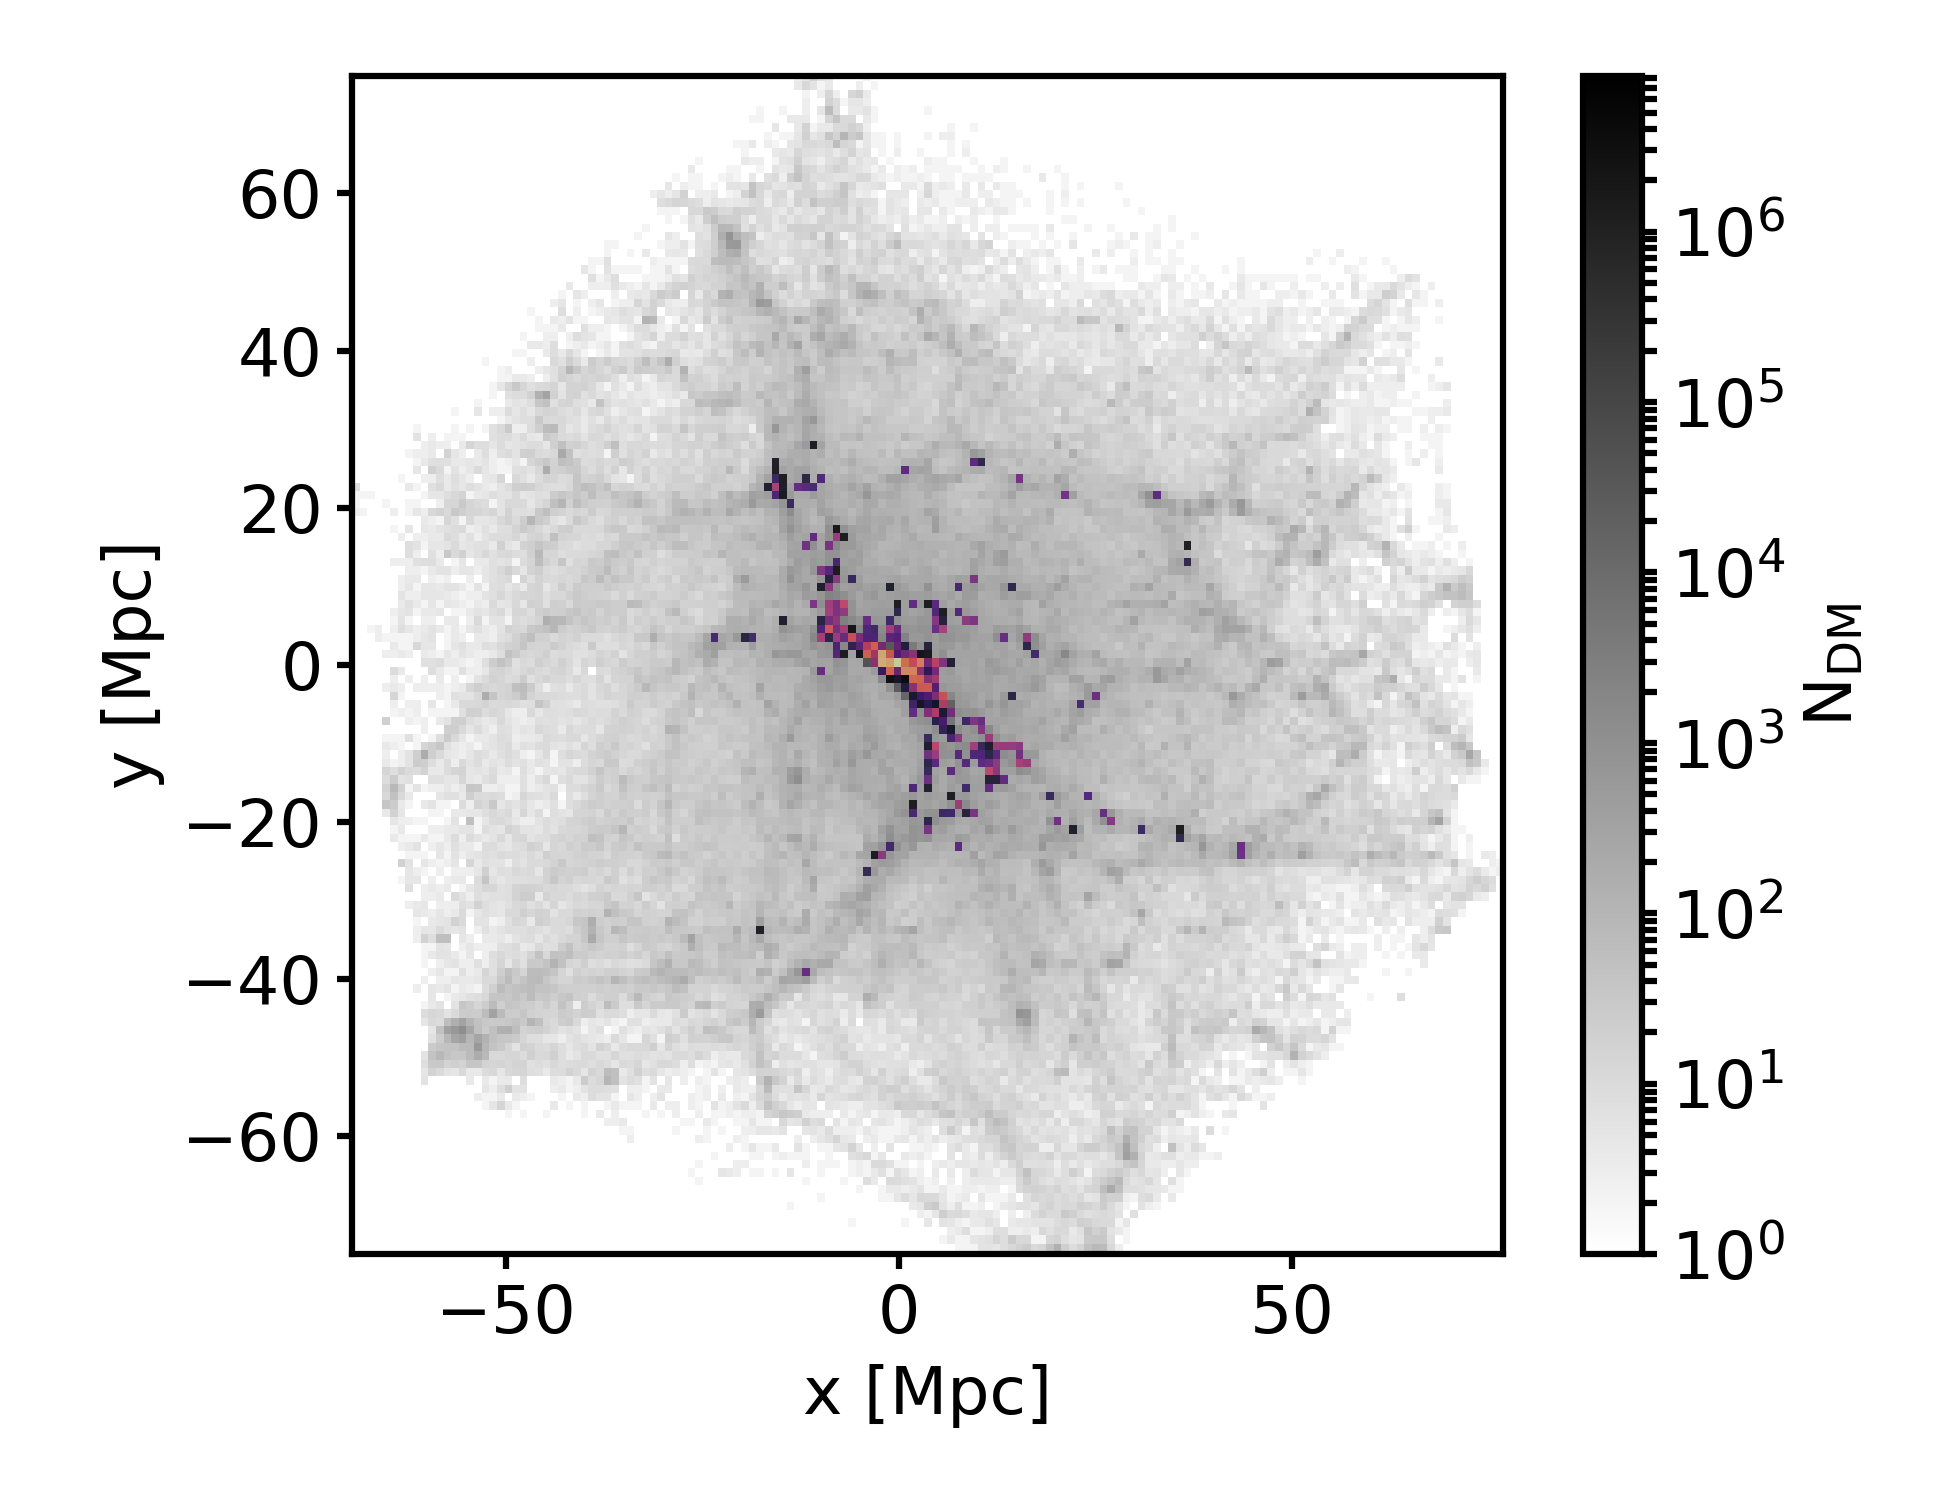
\includegraphics[width=\textwidth]{plots/Auriga/DM_and_stars_xy_distribution.png}
	    \label{fig:DM_stars_xy}
    \end{subfigure}
    
    \begin{subfigure}[b]{0.8\textwidth}
    \centering
    	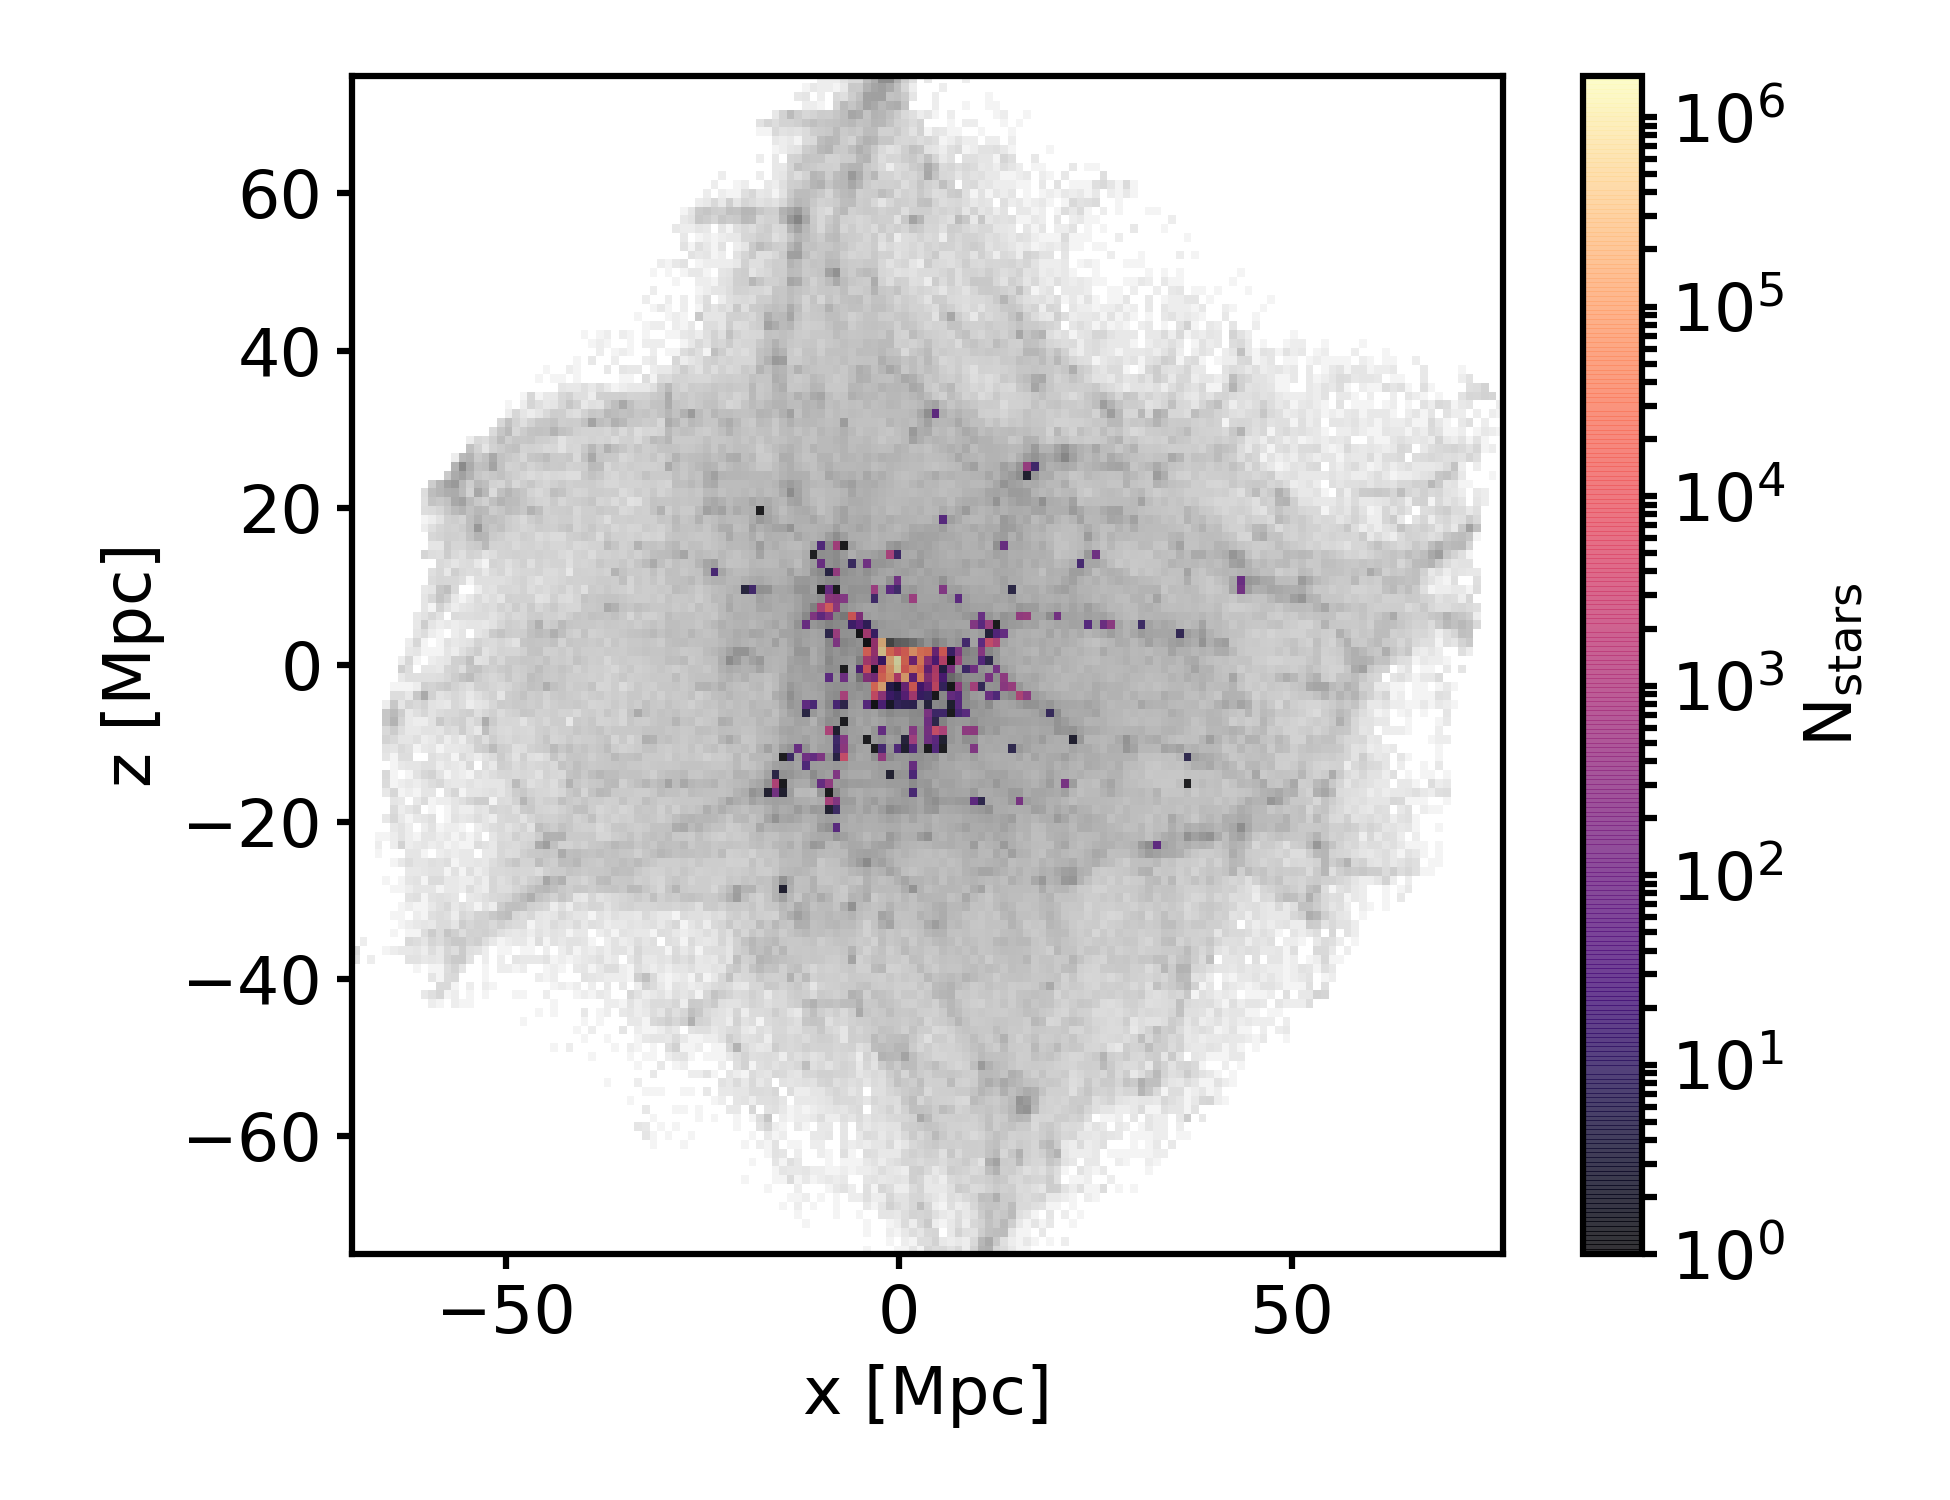
\includegraphics[width=\textwidth]{plots/Auriga/DM_and_stars_xz_distribution.png}
    	\label{fig:DM_stars_xy}
    \end{subfigure}
    \caption{\ac{DM} (grey) and stellar (colors) particle distribution of the whole simulation Auriga24 at $\textit{z}=0$. The \ac{DM} forms the cosmic web, where the mass gathers along its filaments. Baryonic matter also follows these structures. At the most massive parts of the \ac{DM} distribution, the most stellar particles fell in. This structure is typical of hydrodynamical galaxy simulations.}\label{fig:DM_stars_AU24}
\end{figure}
In Figure \ref{fig:DM_stars_AU24}, we show the distribution of \ac{DM} in grey and stars in colors of one selected simulated galaxy (halo 24). The most bound particle is chosen to be the center at $(x,y,z) = (0,0,0)$. The filaments of the \ac{DM} distribution are clearly visible. The stellar particles settle along these filaments and clump inside the densest \ac{DM} structures. 

\subsubsection{Auriga}\label{subsubsec:auriga_intro}
Auriga is a magnetohydrodynamical zoom-in simulation of an isolated \ac{MW} like galaxy. It is build with the moving-mesh AREPO \citep{AREPO} code and includes galaxy physics, active galactic nuclei feedback and magnetic fields. Its goal is to match the observables of the \ac{MW} today and to produce its history which can be compared to observations of spiral galaxies in earlier stages of development. All 30 galaxies are run in normal resolution (\ac{DM} particle mass: $m_\mathrm{DM} = 3\cdot10^5$; Baryonic matter particle mass: $m_\mathrm{b} = 5\cdot10^4$) and 3 selected are run in low ($m_\mathrm{DM} = 2\cdot10^6$; $m_\mathrm{b} = 4\cdot10^5$) and high resolution ($m_\mathrm{DM} = 4\cdot10^4$; $m_\mathrm{b} = 6\cdot10^3$) as well \citep{AurigaGrand}. They are consistent over these three resolution levels and therefore do not rely on numerical parameters but only on physical. Auriga is one of the first simulations where this is accomplished. The snapshots go from redshift $127$, which is close to the beginning of the universe, to redshift $0$, today.  At redshift $z= 0$, different galaxy shapes have evolved. Most of them are spirals but a few are in a merger process. All galaxies have a rich merger history. \citet{AurigaGrand} finds that many properties of the \ac{MW} and \ac{MW} like external galaxies are reproduced by these simulations, such as the mass distribution and the circularity distribution. Others are found to be matching within certain limits, such as the star formation rate–stellar mass relation matches for low redshift $z<1$ but still results in consistent present-day metallicities, mean stellar ages and colours. The set-up and the results of this set of simulations make Auriga one of the most advanced and comprehensive magneto-hydrodynamical galaxy simulations and a very fruitful sample to carry out our investigations. \\
\begin{figure}[htbp]
\captionsetup{format=plain}
    \centering
    \begin{subfigure}[b]{0.8\textwidth}
	    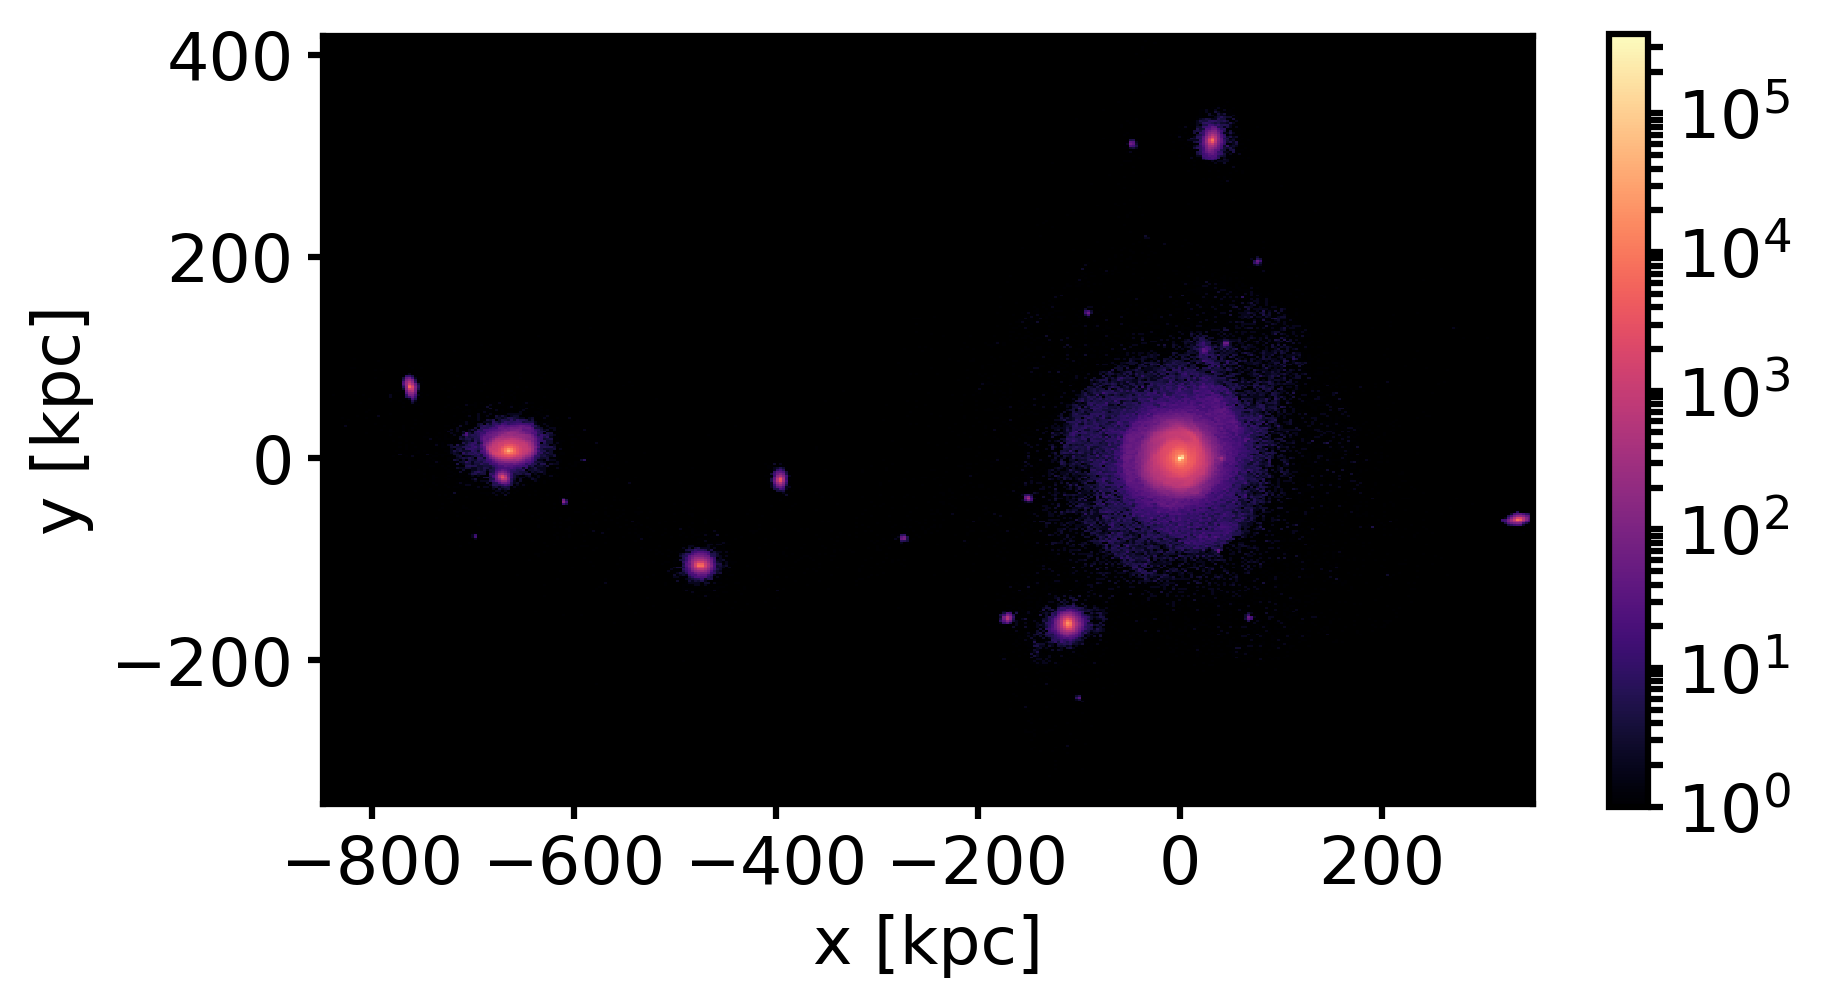
\includegraphics[width=\textwidth]{plots/Auriga/Au24_stars_xy_distribution_halo0.png}
	    \label{fig:Au24_stars_xy}
    \end{subfigure}
    
    \begin{subfigure}[b]{0.8\textwidth}
    \centering
    	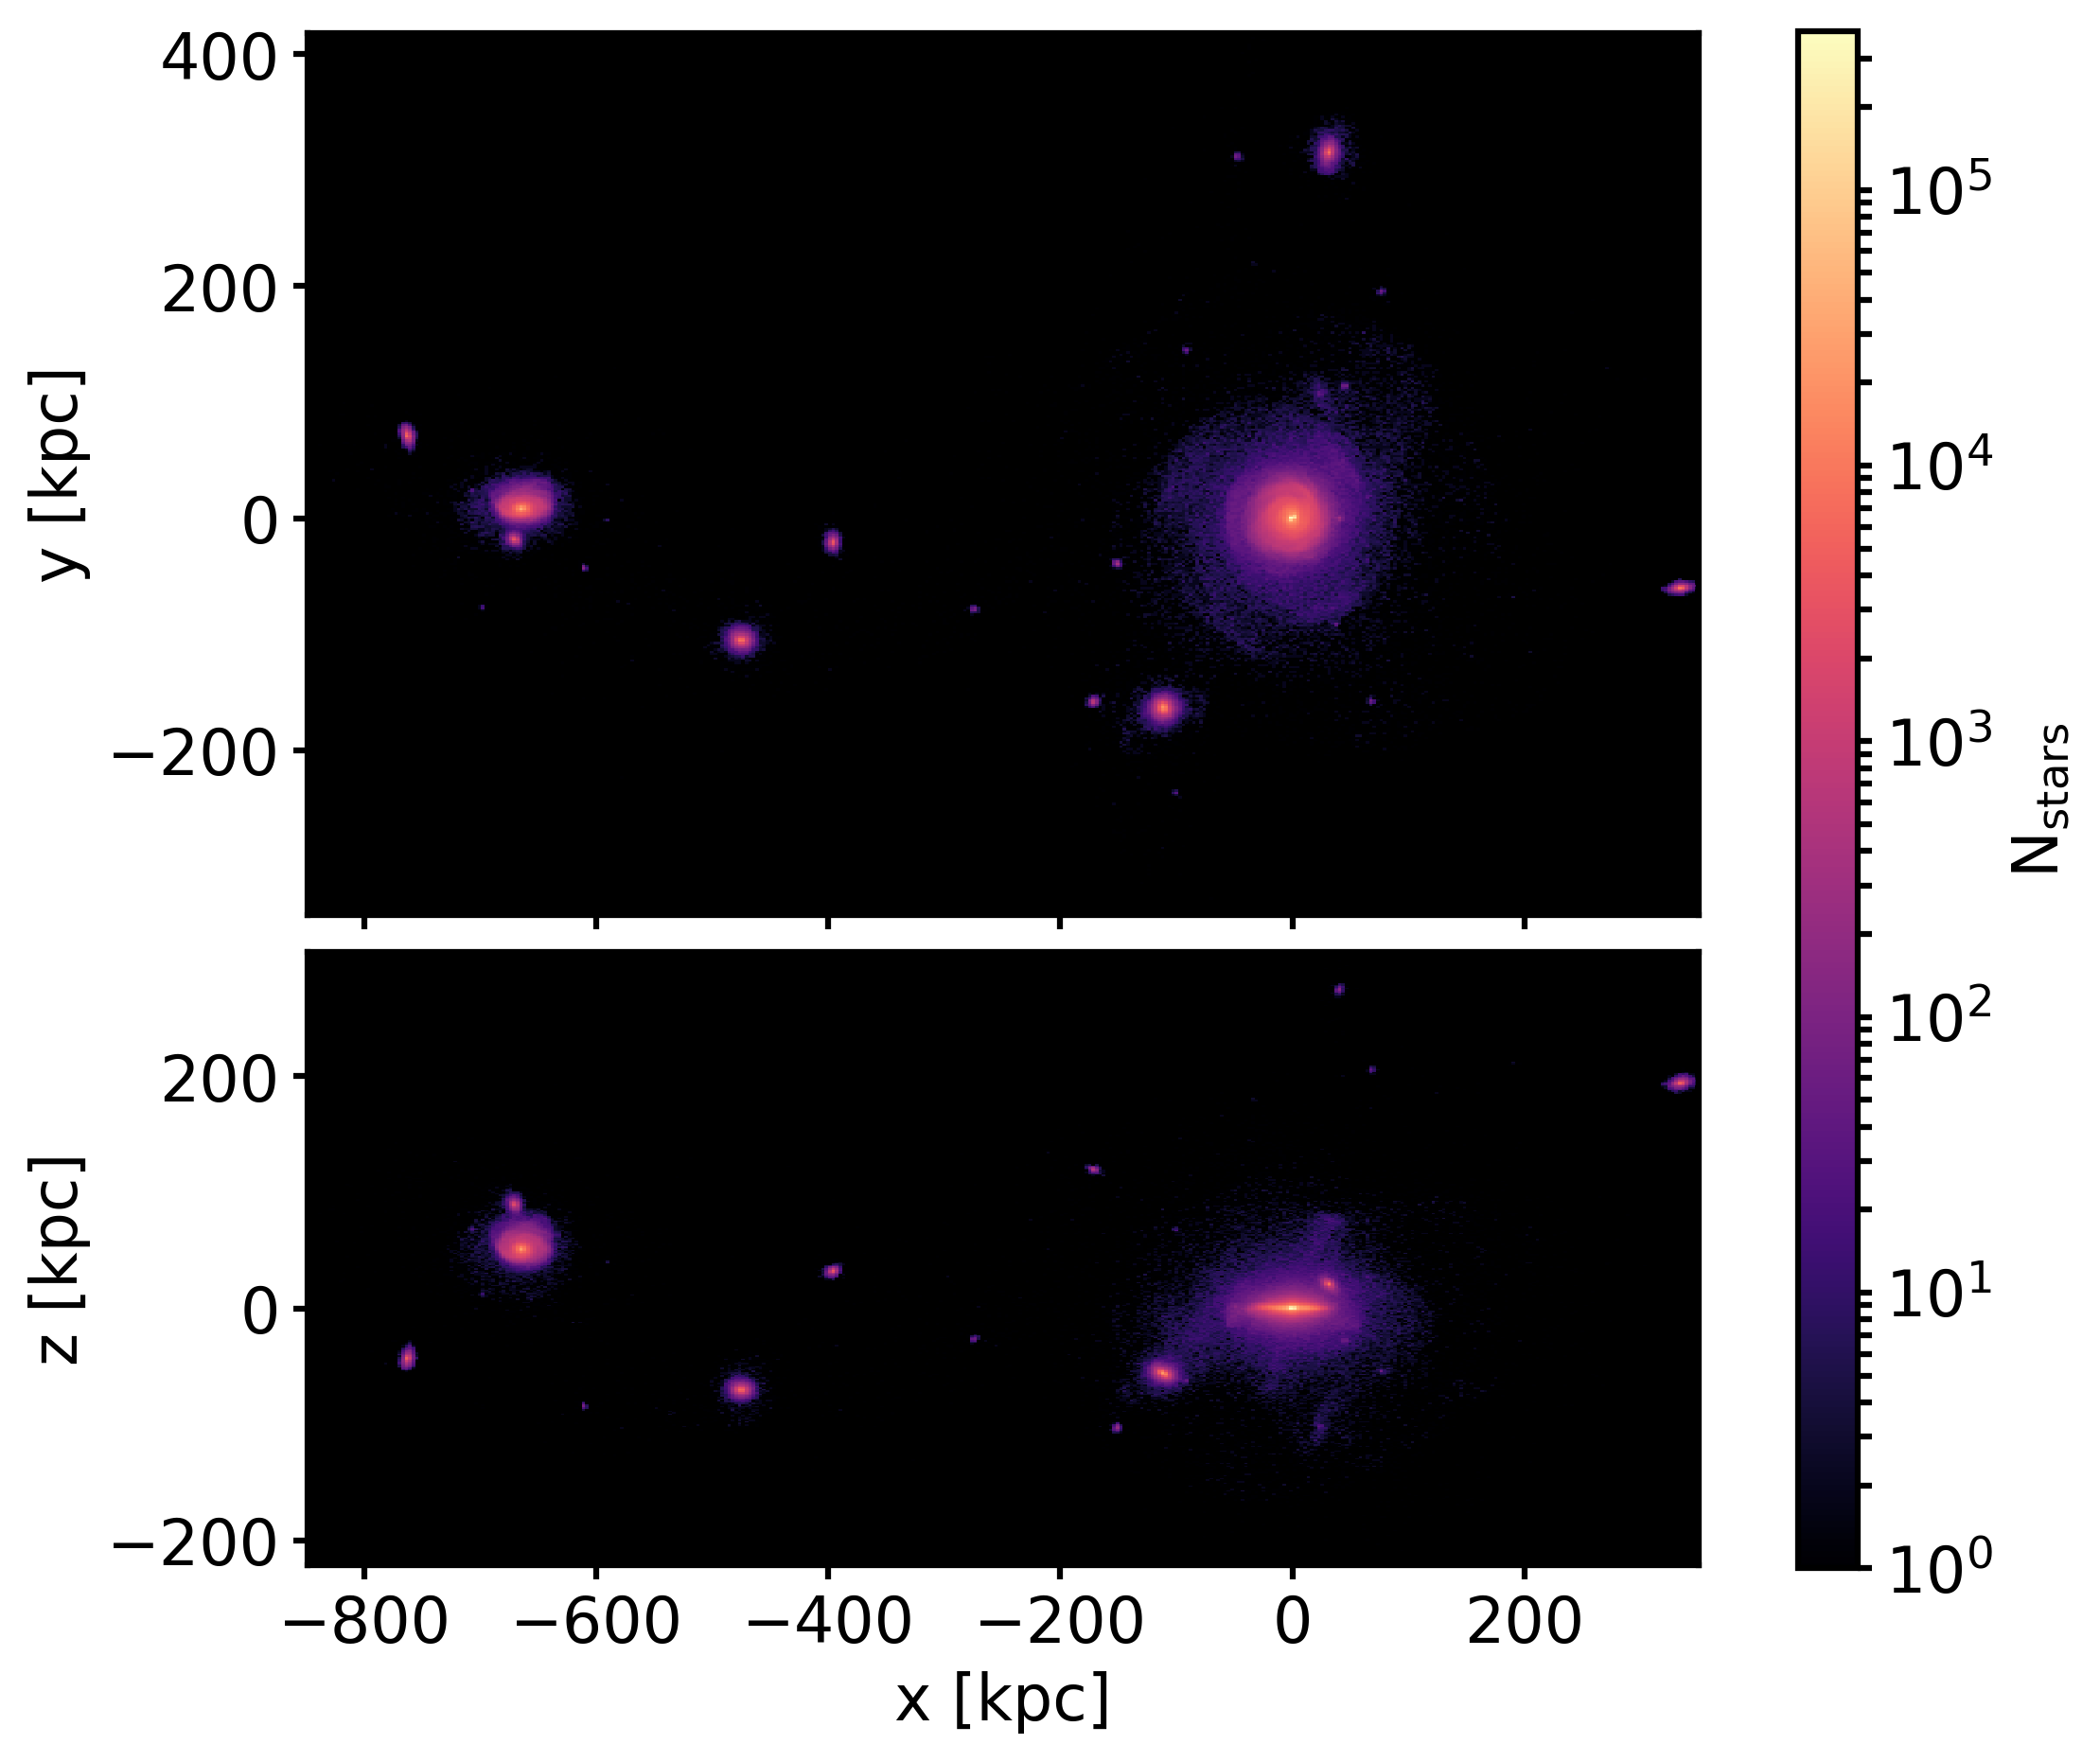
\includegraphics[width=\textwidth]{plots/Auriga/Au24_stars_xz_distribution_halo0.png}
    	\label{fig:Au24_stars_xz}
    \end{subfigure}
    \caption{Stellar distribution of 0th halo at $\textit{z}=0$. The main galaxy is centered at $(0,0,0)$. There are many \acp{DG} around the main galaxy which will eventually merge with it. In the evolution of the simulations, this galaxy has build up mass by merging with \acp{DG}. This mass build up is assumed for and observed in real galaxies.}\label{fig:Stars_AU24}
\end{figure}
\\In Figure \ref{fig:Stars_AU24}, we present the distribution of stellar particles in $x-y$ and $x-z$ direction of the main galaxy in halo 24 and its associated \acp{DG} at redshift $z=0$. Over the course of time, many \acp{DG} already merged with the main galaxy. These make up some of the galaxy's mass and the \ac{DG} stars involved in these mergers are investigated in Section \ref{sec:Dynamics}.\\
\begin{figure}[htbp]
\captionsetup{format=plain}
    \centering
    \begin{subfigure}[b]{0.8\textwidth}
	    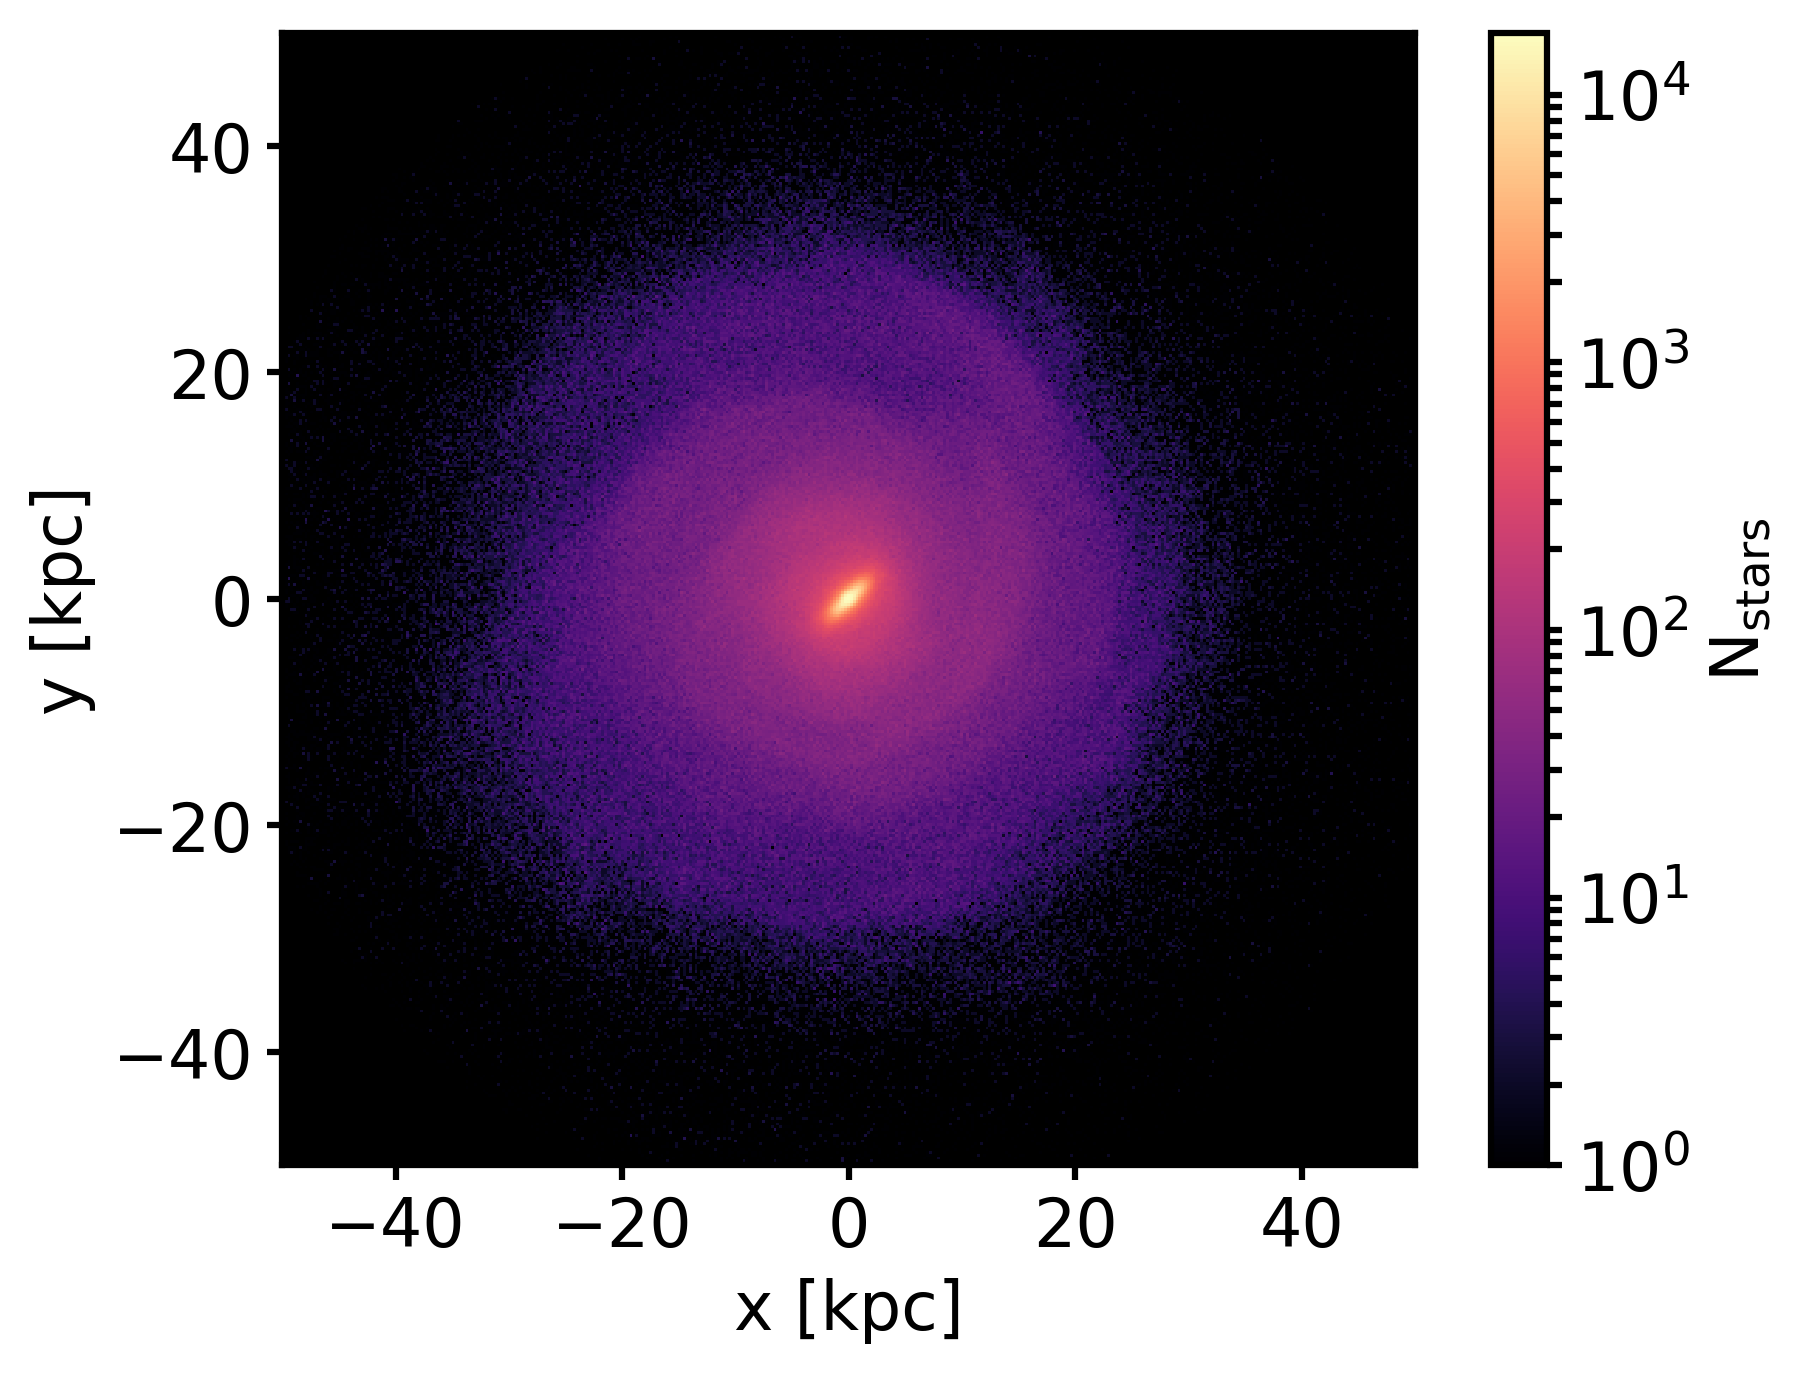
\includegraphics[width=\textwidth]{plots/Auriga/Au24_stars_xy_distribution_halo0_zoomin.png}
	    \label{fig:Au24_stars_xy_zoomin}
    \end{subfigure}
    
    \begin{subfigure}[b]{0.8\textwidth}
    \centering
    	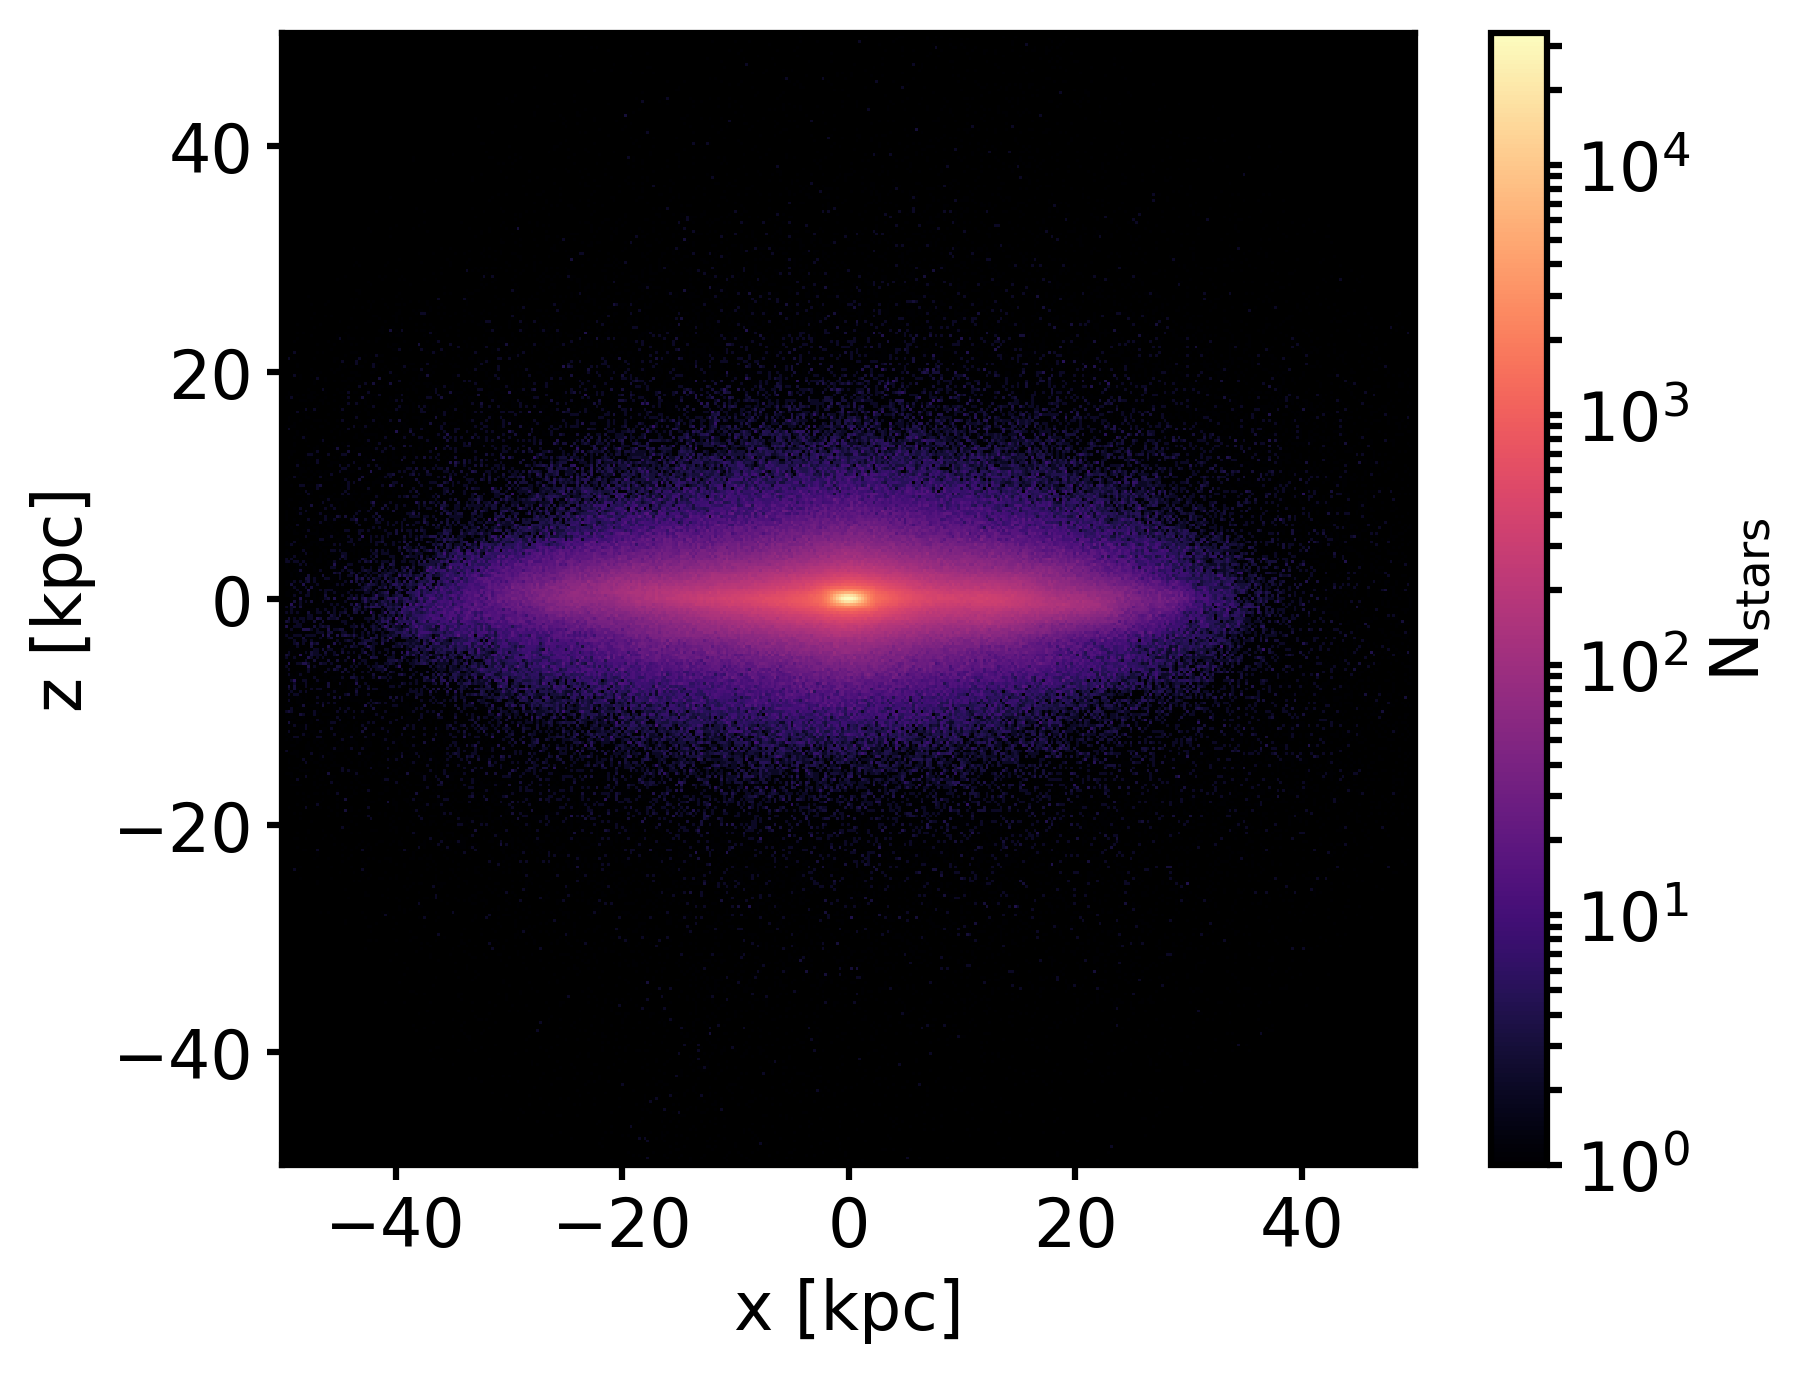
\includegraphics[width=\textwidth]{plots/Auriga/Au24_stars_xz_distribution_halo0_zoomin.png}
    	\label{fig:Au24_stars_xz_zoomin}
    \end{subfigure}
    \caption{Stellar distribution of main galaxy at $\textit{z}=0$. In the upper panel, the galaxy is seen face-on. There, the presence of non-axisymmetric substructure such as spiral arms and a bar is visible. In the lower panel it seen is edge-on. Disk and bulge are clearly present and a close \ac{DG} is visible.}\label{fig:Stars_AU24_zoomin}
\end{figure}
\\A face-on and edge-on view of the main galaxy is presented in Figure \ref{fig:Stars_AU24_zoomin}. We can see axisymmetric features such as bulge and disk and clear non-axisymmetric features such as a bar and spiral arms. This galaxy resembles the \ac{MW} and other late-type galaxies.
\subsection{Fitting axisymmetric potential models}\label{subsec:best_fit_pot}
We require the best fit potential model of this galaxy to be an analytic, axisymmetric, multi-component potential so that we consider this simulations as observers treat external galaxies, since they mostly fit external galaxies with these models (e.g. \citealp{Geehan...Andromedapot...2006}. We need to point out that the galaxy evolved not isolated but went through many mergers and therefore its potential is neither analytic nor axisymmetric but has a lot of substructure. The fit is only an approximation. Also the simulation is self-consistent so changes in potential influence the velocities of the objects inside and changes on the positions of the objects will change the gravitational potential. Since we fit a potential to each snapshot we have a time-dependent potential. The routine and results in this Section are for the $z=0$ snapshot but the same routine was applied for all snapshots since a lookback time of \SI{10.5}{Gyr}. We also need to include a disk and bulge decomposition which is not natural in a cosmological simulation. As the gas evolves in cells, we cannot calculate its density easily. Therefore, we do not consider it in our potential fits. Since we want to recreate observers way of looking at galaxies we do not need to include gas as observers in e.g. Multi-Gaussian Expansion fits \citep{MGE...Monnet, MGE...Emsellem}, that are used in Jeans modelling \citep{Cappellari...Jeans....2008, Glenn....einsteincross...2010}, also only take stellar light into account. 

\subsubsection{About the gravitational potential}\label{subsubsec:pot_theory}
The distribution of stars can be described by their \ac{DF}, $f(\mathbf{x}, \mathbf{v})$ which describes the observed positions and velocities of the stars. They can act as tracers of the gravitational potential $\Phi(\mathbf{x})$. Stars in the disk and the stellar halo are to an extremely good approximation a "collisionless fluid". For these stars, the \ac{CBE} describes their motions: 
\begin{align}\label{eq:CBE}
    \frac{\mathrm{d}f}{\mathrm{d}t} &= \frac{\partial f}{\partial t} + \frac{\partial f}{\partial \mathbf{x}} \cdot \frac{\mathrm{d}\mathbf{x}}{\mathrm{d}t} + \frac{\partial f}{\partial \mathbf{v}} \cdot \frac{\mathrm{d}\mathbf{v}}{\mathrm{d}t}\\
    &= \frac{\partial f}{\partial t} + \bm{\nabla}_x f \cdot \mathbf{v} + \bm{\nabla}_v f \cdot \mathbf{a} = 0.
\end{align}
Applying Newton's gravitational law $\mathbf{F} = -m\bm{\nabla}\Phi(\mathbf{x}) = m\mathbf{a}$ to the last part of the equation and taking the Poisson equation into account to connect $\Phi(\mathbf{x})$ with the total mass we get the important equations:

\begin{empheq}[box=\fbox]{alignat=2}
  &\mathrm{CBE:} \quad&\frac{\mathrm{d}f}{\mathrm{d}t} = \frac{\partial f}{\partial t} + \bm{\nabla}_x f \cdot \mathbf{v} - \bm{\nabla}_v f \cdot \bm{\nabla}_x \Phi(\mathbf{x}) \label{eq:CMB_phi}\\
  &\mathrm{Poisson:}\quad&\bm{\nabla} \cdot \bm{\nabla} \Phi(\mathbf{x})= \bm{\nabla}^2 \Phi(\mathbf{x}) =4\pi G \rho(\mathbf{x}) \label{eq:Poisson}
\end{empheq}
with the gravitational constant $G$ and the total mass density of stars, gas and \ac{DM}, $\rho(\mathbf{x})$. 
If the system is in "steady state", $\partial f/\partial t = 0$, distribution functions that are functions of the \ac{IoM} solve Equation \ref{eq:CMB_phi} (see Section \ref{sec:Dynamics}). The Poisson equation, Equation \ref{eq:Poisson}, is used to link densities and potentials in the upcoming descriptions of the potentials of the single components and presents a direct link between the gravitational potential and the total mass. 

\subsubsection{galpy - A python package for galactic dynamics}\label{subsubsec:galpy}
galpy \citep{Bovy...galpy...2015} is a well tested and well documented python package for galactic dynamics that is being developed on \url{http://github.com/jobovy/galpy}. The latest documentation can be found at \url{http://galpy.readthedocs.org/en/latest/}. It includes analytic spherical, axisymmetric and ellipsoidal triaxial potentials and fast routines, additionally implemented in C, for the calculation of orbits, action-angles and \acp{DF}. galpy has its own internal units which have to be considered and understood before using it.
\\In this work, we first fit a set of analytic potentials to the simulation which is described in the remainder of this Section. Then, we calculate actions of accreted \acp{GC} in a variety of potentials in galpy and investigate the results in the next Section. 

\subsubsection{Component decomposition}\label{subsubsec:decomp}
To fit a potential to each component, we first need to decompose the different parts. We assume that all \ac{DM} particles belonging to the main galaxy make up its halo. The stellar particles belong to either the central spheroid or the disk. We distinguish these components by the use of the circularity parameter \citep{Abadi...circularity...2003}
\begin{equation}\label{eq:circularity}
    \epsilon = \frac{L_z}{L_{z,max}(E)}
\end{equation}
where $L_{z,max}(E)$ is the maximum angular momentum allowed for the orbital energy $E$. 
$\epsilon = 1$ is a prograde circular orbit in the disc plane. $\epsilon = -1$ is a retrograde circular orbit in the disc plane. $\epsilon \sim 0$ is an orbit with a very low $z$-component of angular momentum which may be highly inclined to the disc spin axis and/or be highly eccentric.  
\begin{SCfigure}
\captionsetup{format=plain}
    \centering
    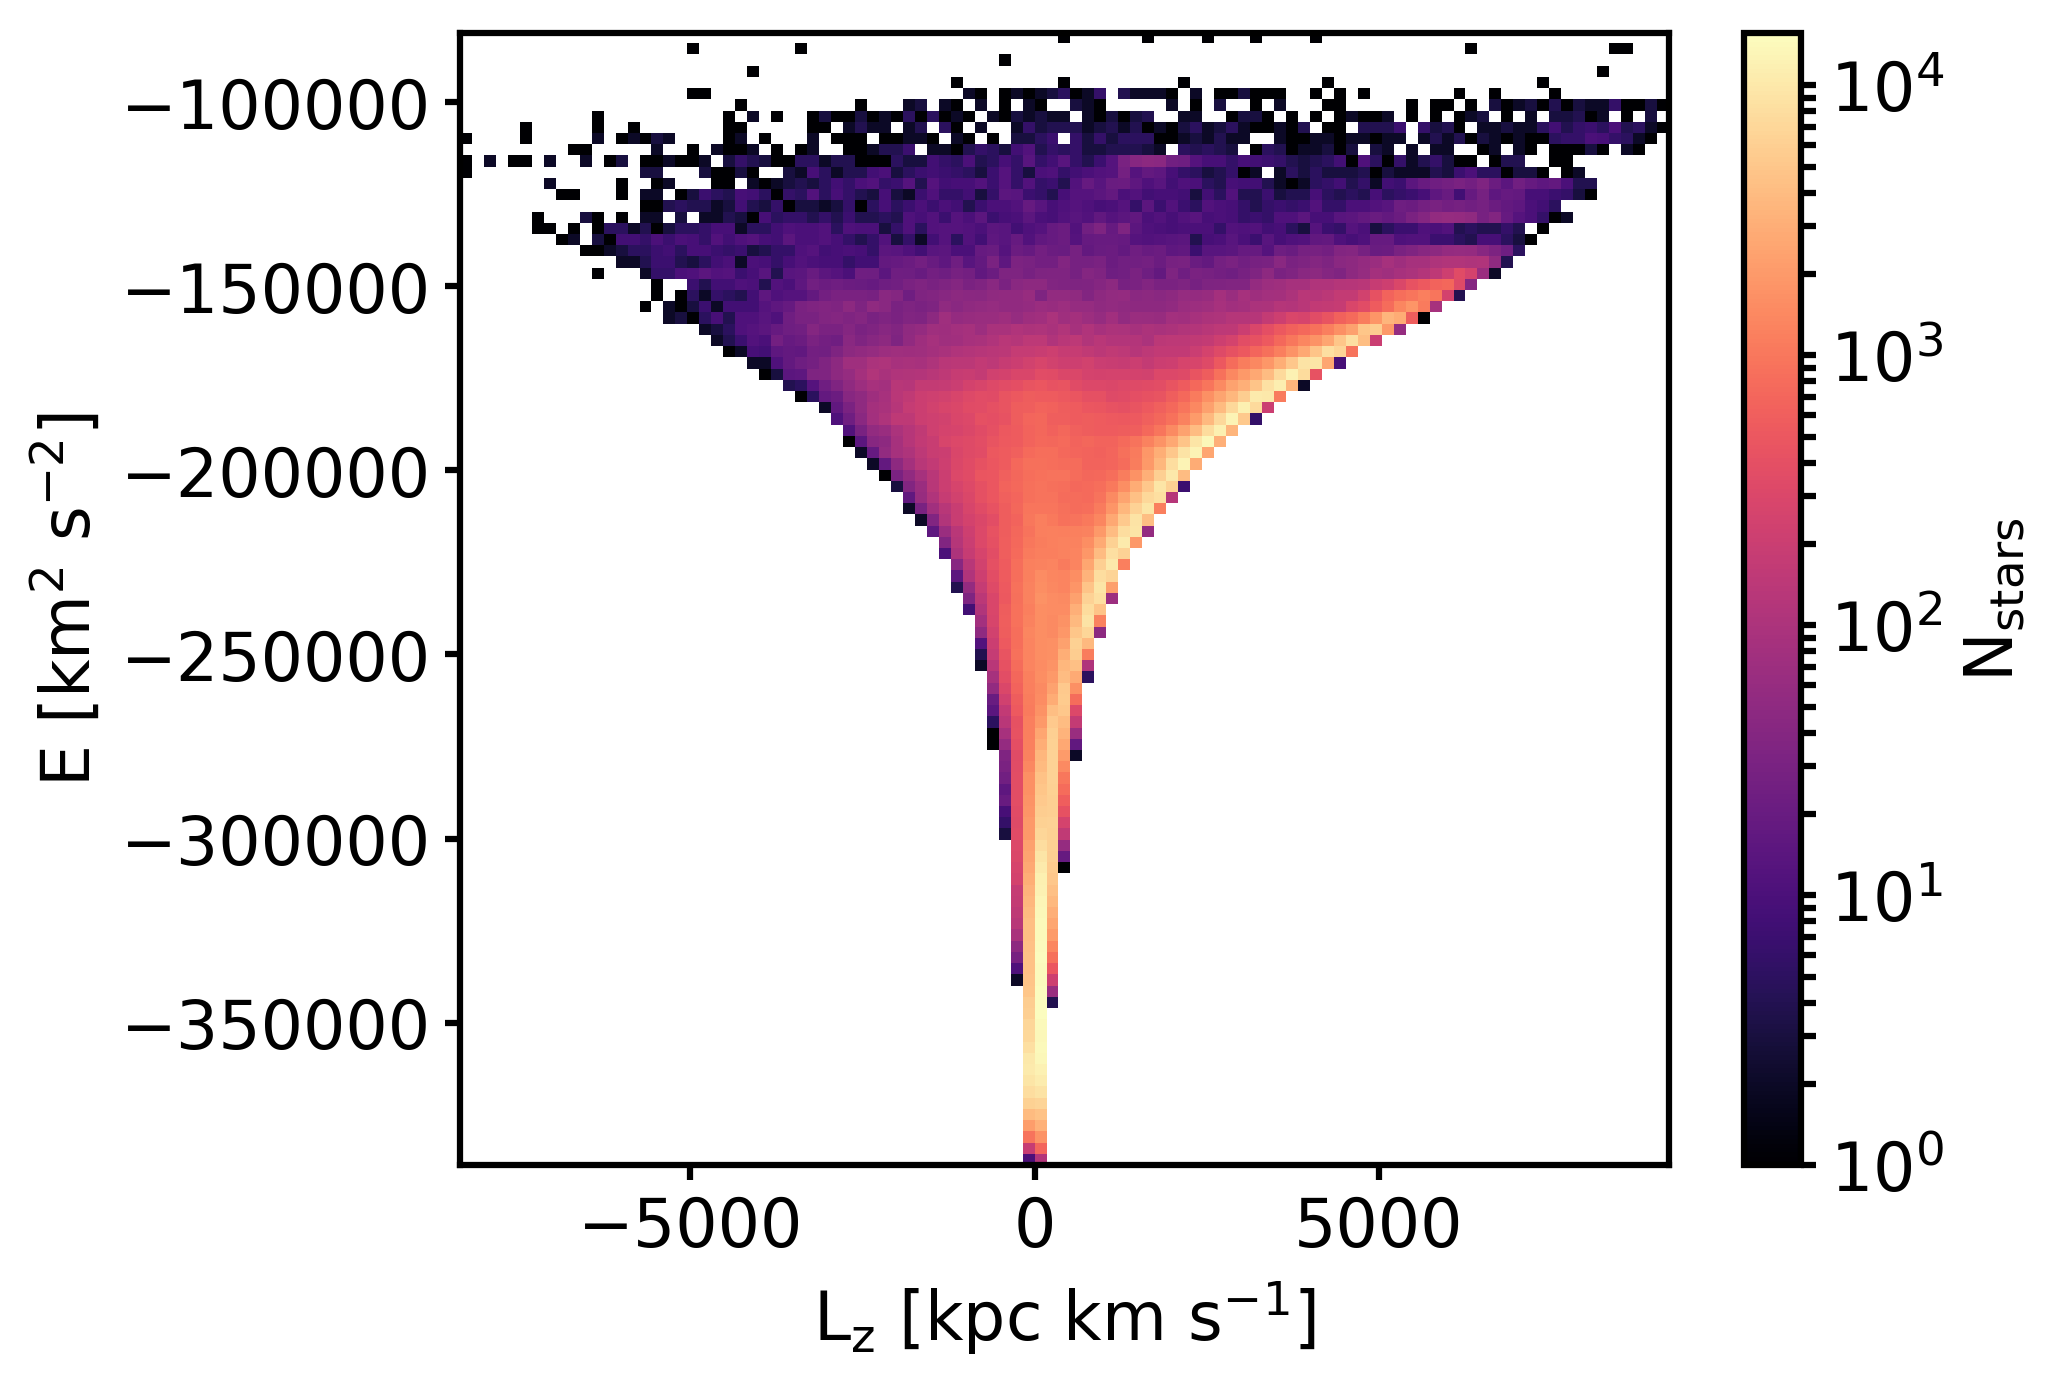
\includegraphics[width = 0.6\textwidth]{plots/Auriga/decomposition_elz_snap_127.png}
    \caption{Energy vs angular momentum of all stellar particles within the galaxy radius. $L_{z,max}$ is the right border of the distribution. Stars which lie close to that edge are therefore disk stars which is very good visible in the overdensity there. \textcolor{red}{Muss Mpc sein in x achse}}
    \label{fig:e_lz_dist}
\end{SCfigure}
\cite{AurigaGrand} uses two different methods two distinguish the components and to get their mass ratio:
\begin{enumerate}
\item Under the assumption, that the bulge has zero net rotation, mirror negative $\epsilon$ as bulge material, the rest belongs to the disk.
\item All particles with $\epsilon > \mathrm{constant}$ are assigned to the disk, where $\mathrm{constant} = 0.7$ is set heuristically.
\end{enumerate}

\cite{AurigaGrand} find that the first method generally overestimates the \ac{D/T} ratio while the second approach underestimates it by choosing only kinematically very cold particles. Since we do not only want to get the mass ratio of \ac{D/T} but also want to tag each particle clearly, we use the second method. Nevertheless, the true assignment lies somewhere between these methods. 
\begin{SCfigure}%[htbp]
\captionsetup{format=plain}
    \centering
    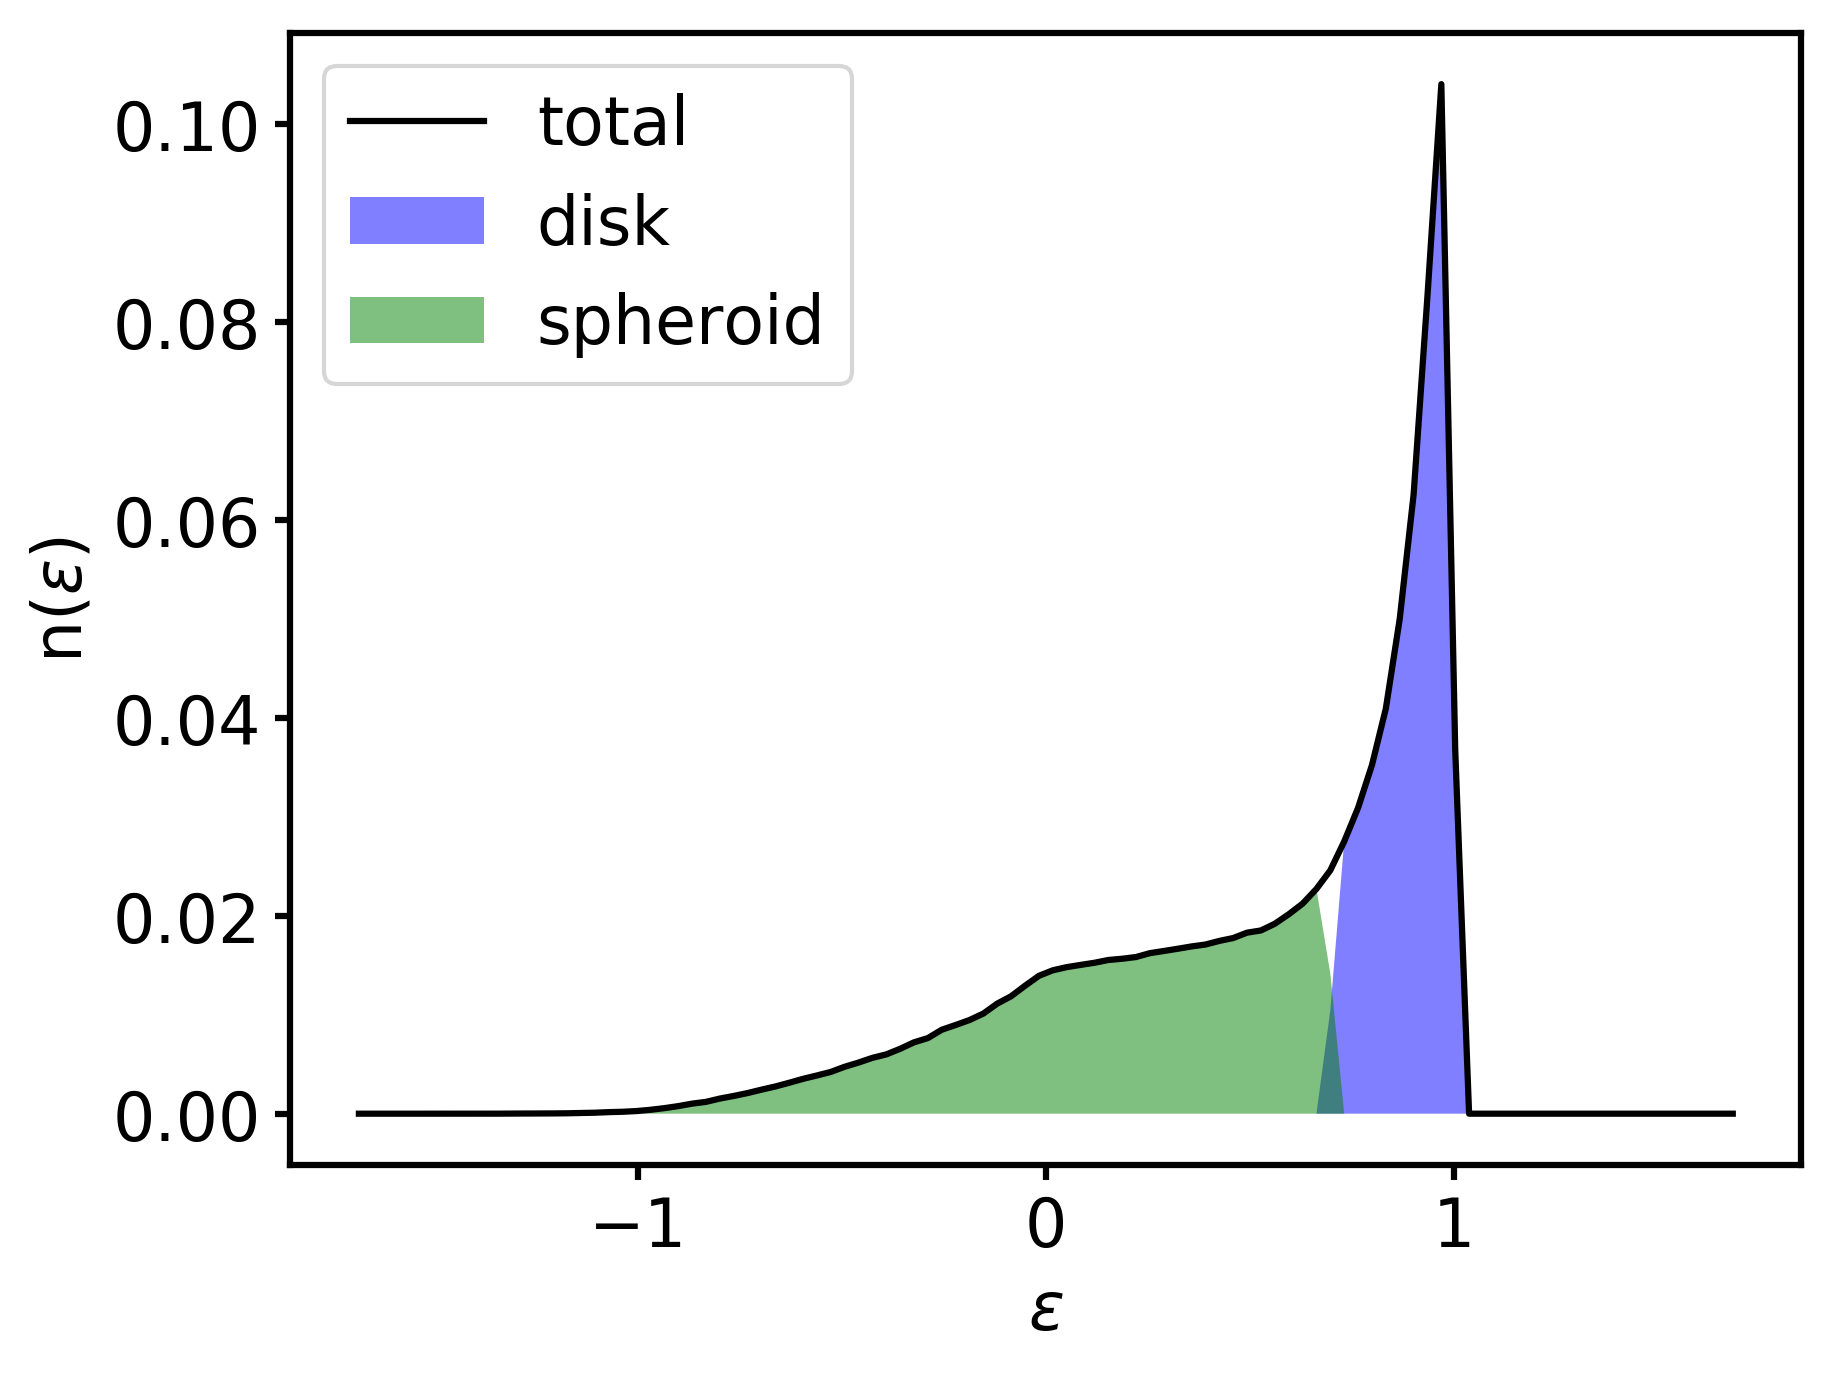
\includegraphics[width=0.6\textwidth]{plots/Auriga/decomposition_snap_127.png}
\caption{Decomposition of stellar disk and spheroid by their circularity. It was carried out for all stellar particles within the galaxy radius. The black line represents the total circularity. The green area is the the spheroid component and the blue is the disk component. The disk particles were selected by having a circularity above 0.7. The disk to total number ratio is 0.47.}\label{fig:decomposition}
\end{SCfigure}
\\In Figure \ref{fig:decomposition}, we show a histogram of the circularity with our decomposition. The blue part is the disk portion while the green part is the spheroid. Together they add up to the black solid line, the total number. The \ac{D/T} ratio is 0.47.
Since we can assign the particles to be in the spheroid or disk easily, we use this composition to find the disk and spheroid where we fit our potential to. 


\subsubsection{Disk potential}\label{subsubsec:disk_pot}
We fit the disk with a \citet{MNprofile} (\acsu{MN}) potential following the profile 
\begin{equation}\label{eq:MND}
\Phi(R,z) = -\frac{GM}{\sqrt{R^2+(a+\sqrt{z^2+b^2})^2}}
\end{equation} 
with scale length $a$ and scale height $b$ which provides a disk with a finite thickness. If $b\rightarrow 0$, the disk will be infinite thin and if $a \rightarrow 0$, the potential has a spherical density distribution. $b/a$ therefore defines the flattening of the system. It is a rather simple model with only small computational costs as forces and densities can be calculated analytically from Equation \ref{eq:MND}. Therefore it is widely used. It has limitations in the mid-plane ($z=0$) at high $R$ as the density behaves as $R^−3$ for $R\gg a$ and the large-radius density fall-off is therefore simply a power-law of $R$ rather than exponential. The \ac{MN} density remains too high at large radii (e.g., at $R\gg15$ kpc for the \ac{MW}) compared to realistic models of galactic disks. 
\\To fit the disk potential, we bin the stellar disk in $(R, z)$ and calculate the density of each bin. Then, we fit the \ac{MN} density to the data using the scipy \citep{scipy....2001} routine optimize.curve\_fit. For the \ac{MN} potential, we have the scale length $a_{\mathrm{MND}}$, the scale height $b_{\mathrm{MND}}$ and the contribution to the total circular velocity $v_{0, \mathrm{MND}}$ at $ R_0 = \SI{8}{kpc}$ as fit parameters. The best fit parameters are listed in Table \ref{tab:pot_best_fit_params}.
\begin{figure}[htbp]
\captionsetup{format=plain}
    \centering
    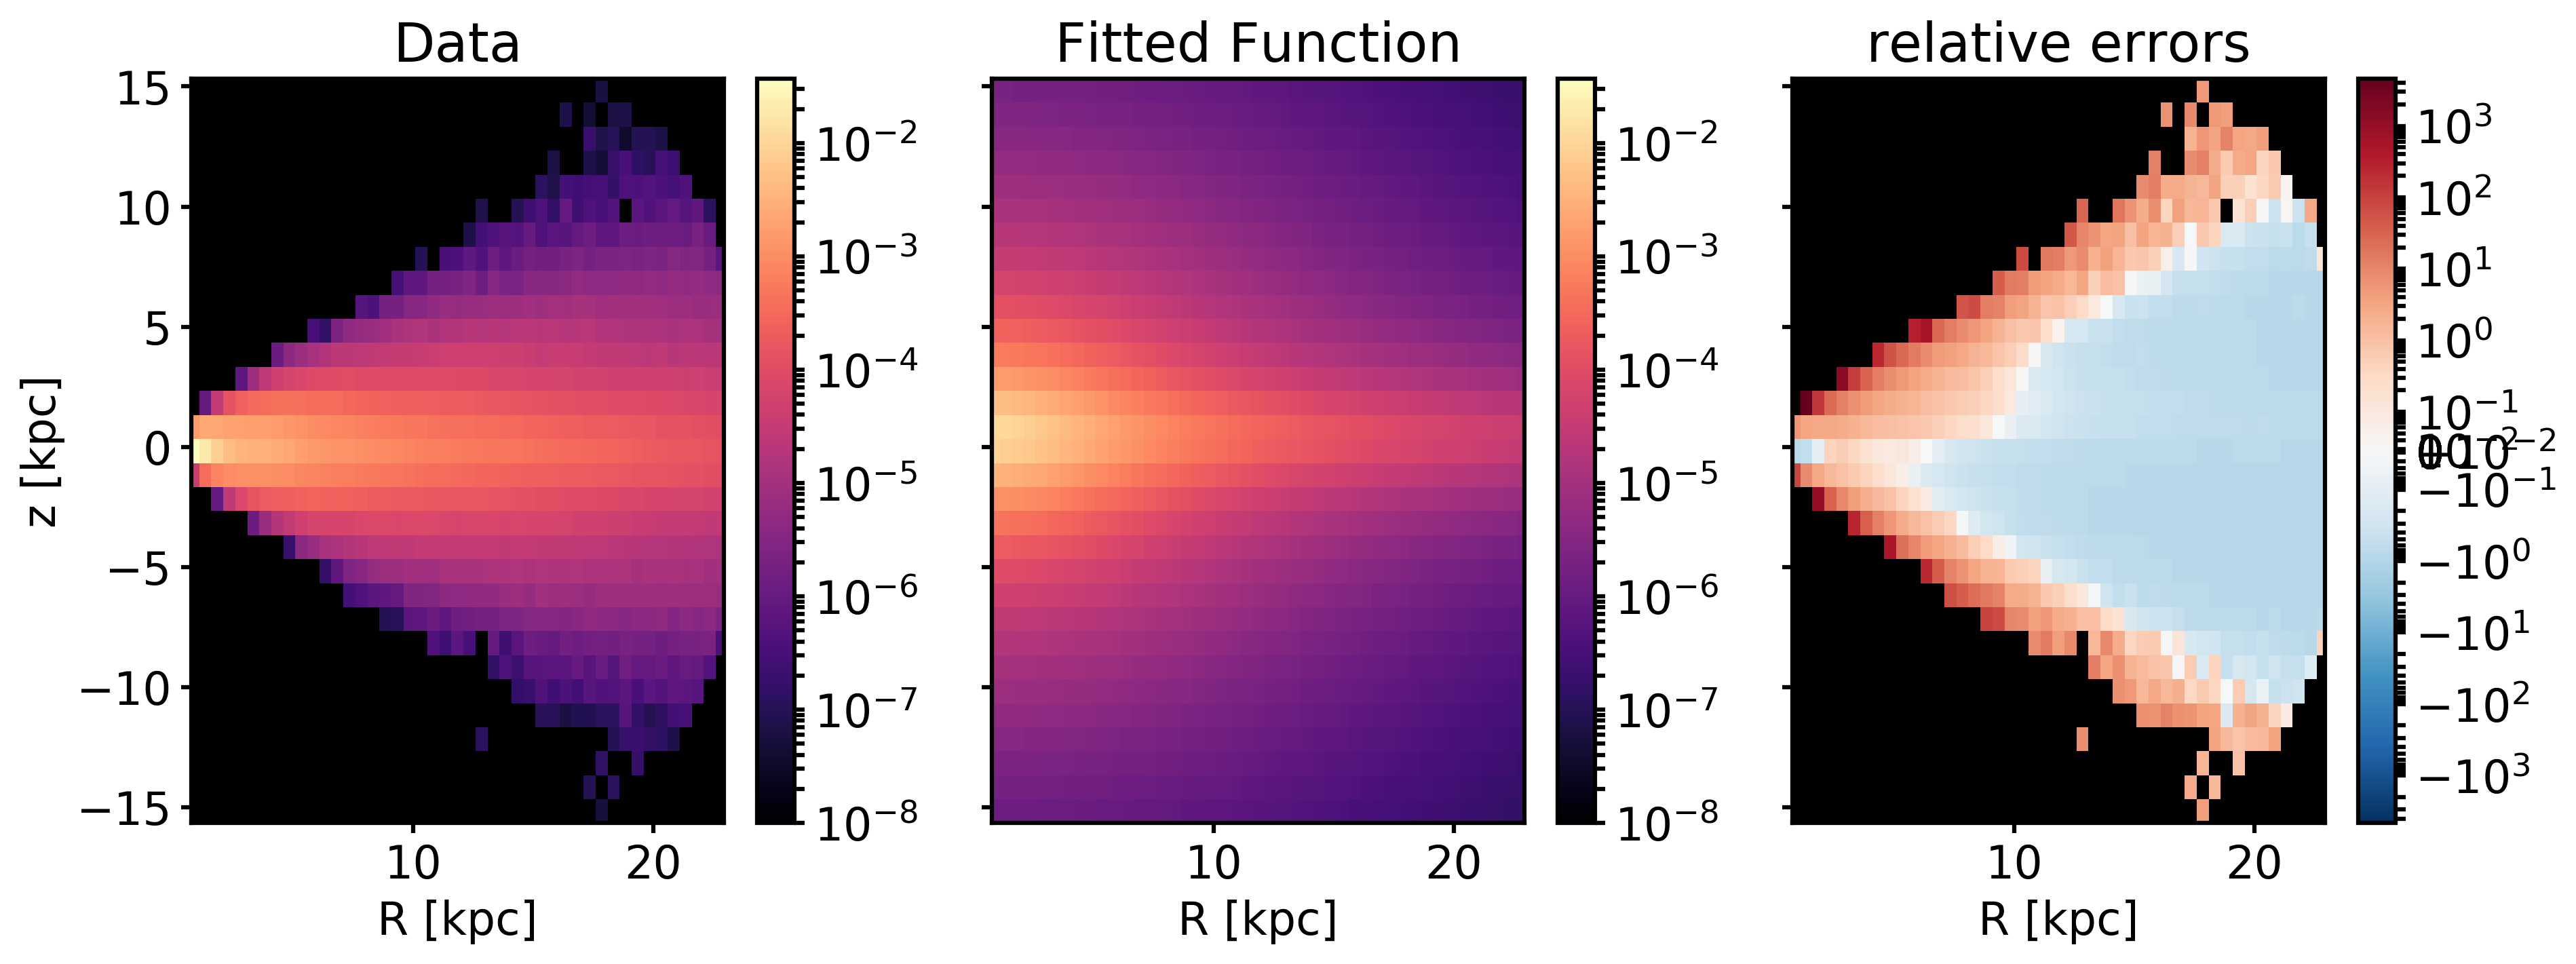
\includegraphics[width = \textwidth]{plots/Auriga/MND_best_fit_snap_127.png}
    \caption{Density fit of the \ac{MN} profile to the disk. \textit{Left panel:} in $(R,z)$ binned mass density of the simulation data. \textit{Middle panel:} in $(R,z)$ binned mass density of the best fit \ac{MN} profile. \textit{Right panel:} relative errors \(\Delta_\rho = (\rho_{\mathrm{fit}}- \rho_{\mathrm{data}})/\rho_{\mathrm{data}}\) of the best fit.}
    \label{fig:MND}
\end{figure}
\\The best fit is shown in Figure \ref{fig:MND}. In the left panel, we see the binned data. Due to the kinematic selection of disk particles, the disk appears to be flaring. This is negligible since the density falls off quickly above an absolute height of \SI{1.5}{kpc}. At the black parts of the histogram, there was no data. Therefore, they weights of the fit lay on the actual disk. In the middle panel, we show the binned density of the best fit \ac{MN} profile. We can clearly see the disk. Since it is an analytic potential, the density can be calculated for every bin in $(R, z)$. In the right panel, the relative errors \(\Delta_\rho = (\rho_{\mathrm{fit}}- \rho_{\mathrm{data}})/\rho_{\mathrm{data}}\) are plotted. In the edges of the data, these errors are very high. This is most probably due to selection effects and cutting the data there while the fitted density is still smooth there. In the disk and outer regions, the relative error is smaller than at the edges. We discuss problems with the disk fit in Section \ref{subsec:wrong_pot_fit}. Even though the errors are quite big, we think this is the best fit of the analytic \ac{MN} potential to the non-analytic and selected-through-decomposition disk. 


\subsubsection{Spheroid potential}\label{subsubsec:spher_pot}
For the central stellar spheroid, we apply a \citet{Hernquistprofile} potential which has the density 
\begin{equation}
    \rho = \frac{M}{2\pi}\frac{a}{r}\frac{1}{(r+a)^3}
\end{equation}
where $M$ is the stellar mass of the spheroid and $a$ is its scale length. It has a gentle power-law cusp and at large radii, it declines like $r^{-4}$. \citet{Hernquistprofile} has shown that it reproduces properties of elliptical galaxies and spherical bulges. 
\\
\begin{SCfigure}
\captionsetup{format=plain}
    \centering
    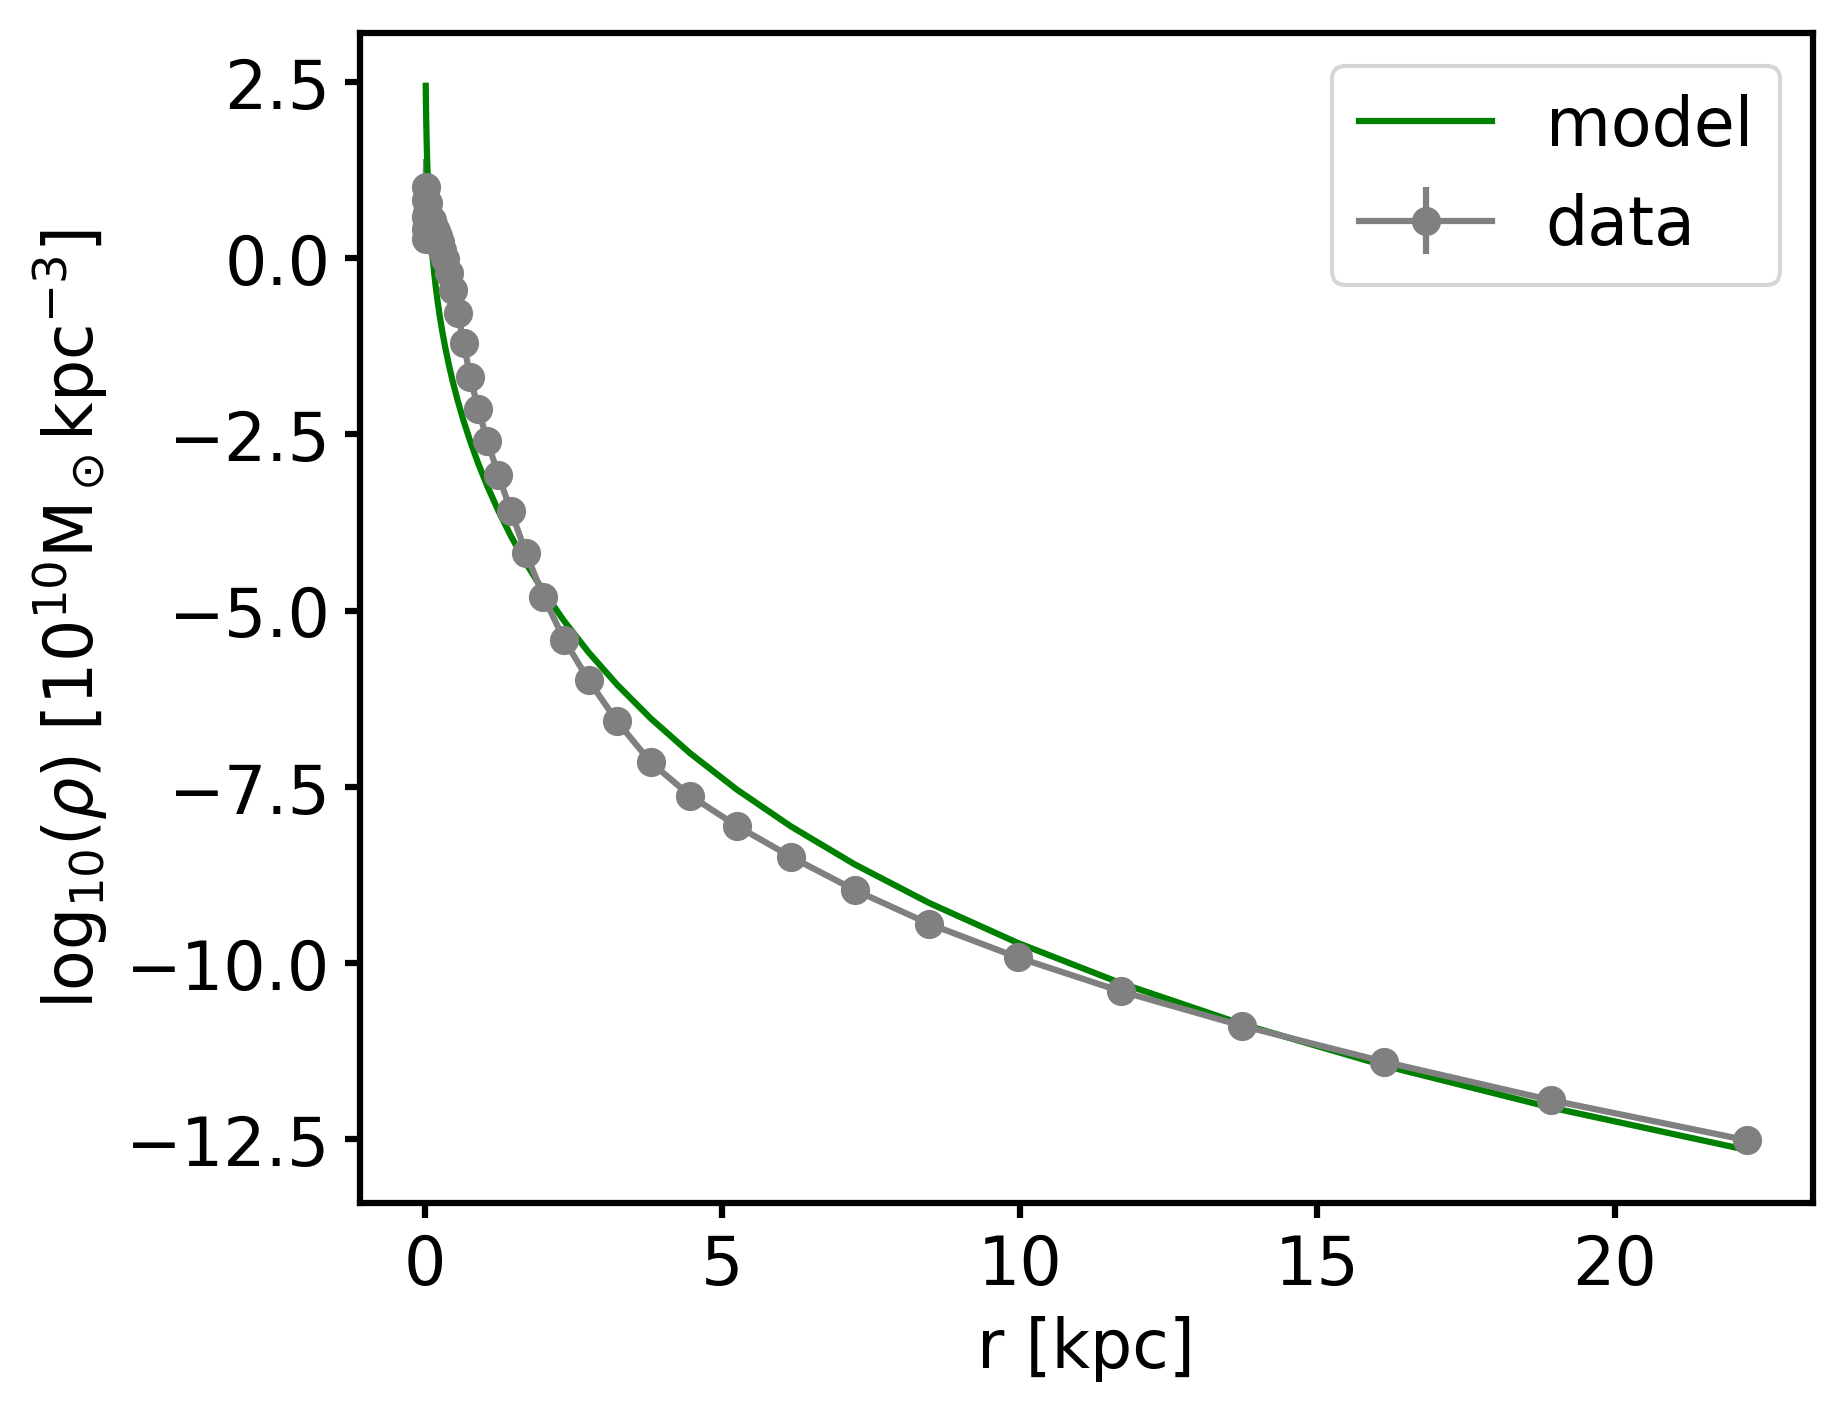
\includegraphics[width=0.7\textwidth]{plots/Auriga/spheroid_density_fit_snap_127.png}
    \caption{Spheroid density: data with errors (grey dots) and best fit (green line). The data is binned logarithmically in r. Their standard deviation is too small to be seen. In the inner part, r $<10$kpc, the density is both under and over estimated. In the outer parts, the fit matches the data.}
    \label{fig:spheroid_fit}
\end{SCfigure}
\\Since the Hernquist density is spherically symmetric, we bin the spheroid particles to logarithmic bins in the spherical radius $r$. The data and best fit densities are shown in Figure \ref{fig:spheroid_fit}. While in the inner part the fit does not match the data too well, in the outer parts it fits. Since most of the particles we investigate in Section \ref{sec:Dynamics} are more far away from the center than \SI{10}{kpc}, the fit is acceptable to carry out this analysis.

\subsubsection{Halo potential}\label{subsubsec:halo_pot}
We model the \ac{DM} halo with a \acsu{NFW} \citep{NFWprofile} profile following the formula 
\begin{equation}
    \rho(r) = \frac{\rho_{crit} \cdot \delta_c}{(r/r_s)(1+r/r_s)^2} = \frac{M}{4 \pi a^3}\frac{1}{(r/a)(1+r/a)^2}
\end{equation} with scale radius $r_s = a$, the critical density $\rho_{crit} = 3H^2 / 8\pi G $, the mass $M$ of the \ac{DM} halo and a characteristic and dimensionless density $\delta_c$ which can be rewritten as \(\rho_{crit}\cdot\delta_c = M/4\pi a^3 \). The \ac{NFW} profile is derived from \ac{DM} only hydrodynamical simulations and found to accurately describe \ac{DM} halos. 
\\All particles in the simulation have a potential value, 'pot',  which is the potential they feel at their position from the total surrounding matter (not only from the host galaxy). Since the total halo (shown in Figure \ref{fig:Stars_AU24}) is isolated and the main matter contribution comes from the main galaxy and its halo, we still consider this a value where we can fit the potential of the analytic model to. 
\begin{figure}[htbp]
\captionsetup{format=plain}
    \centering
    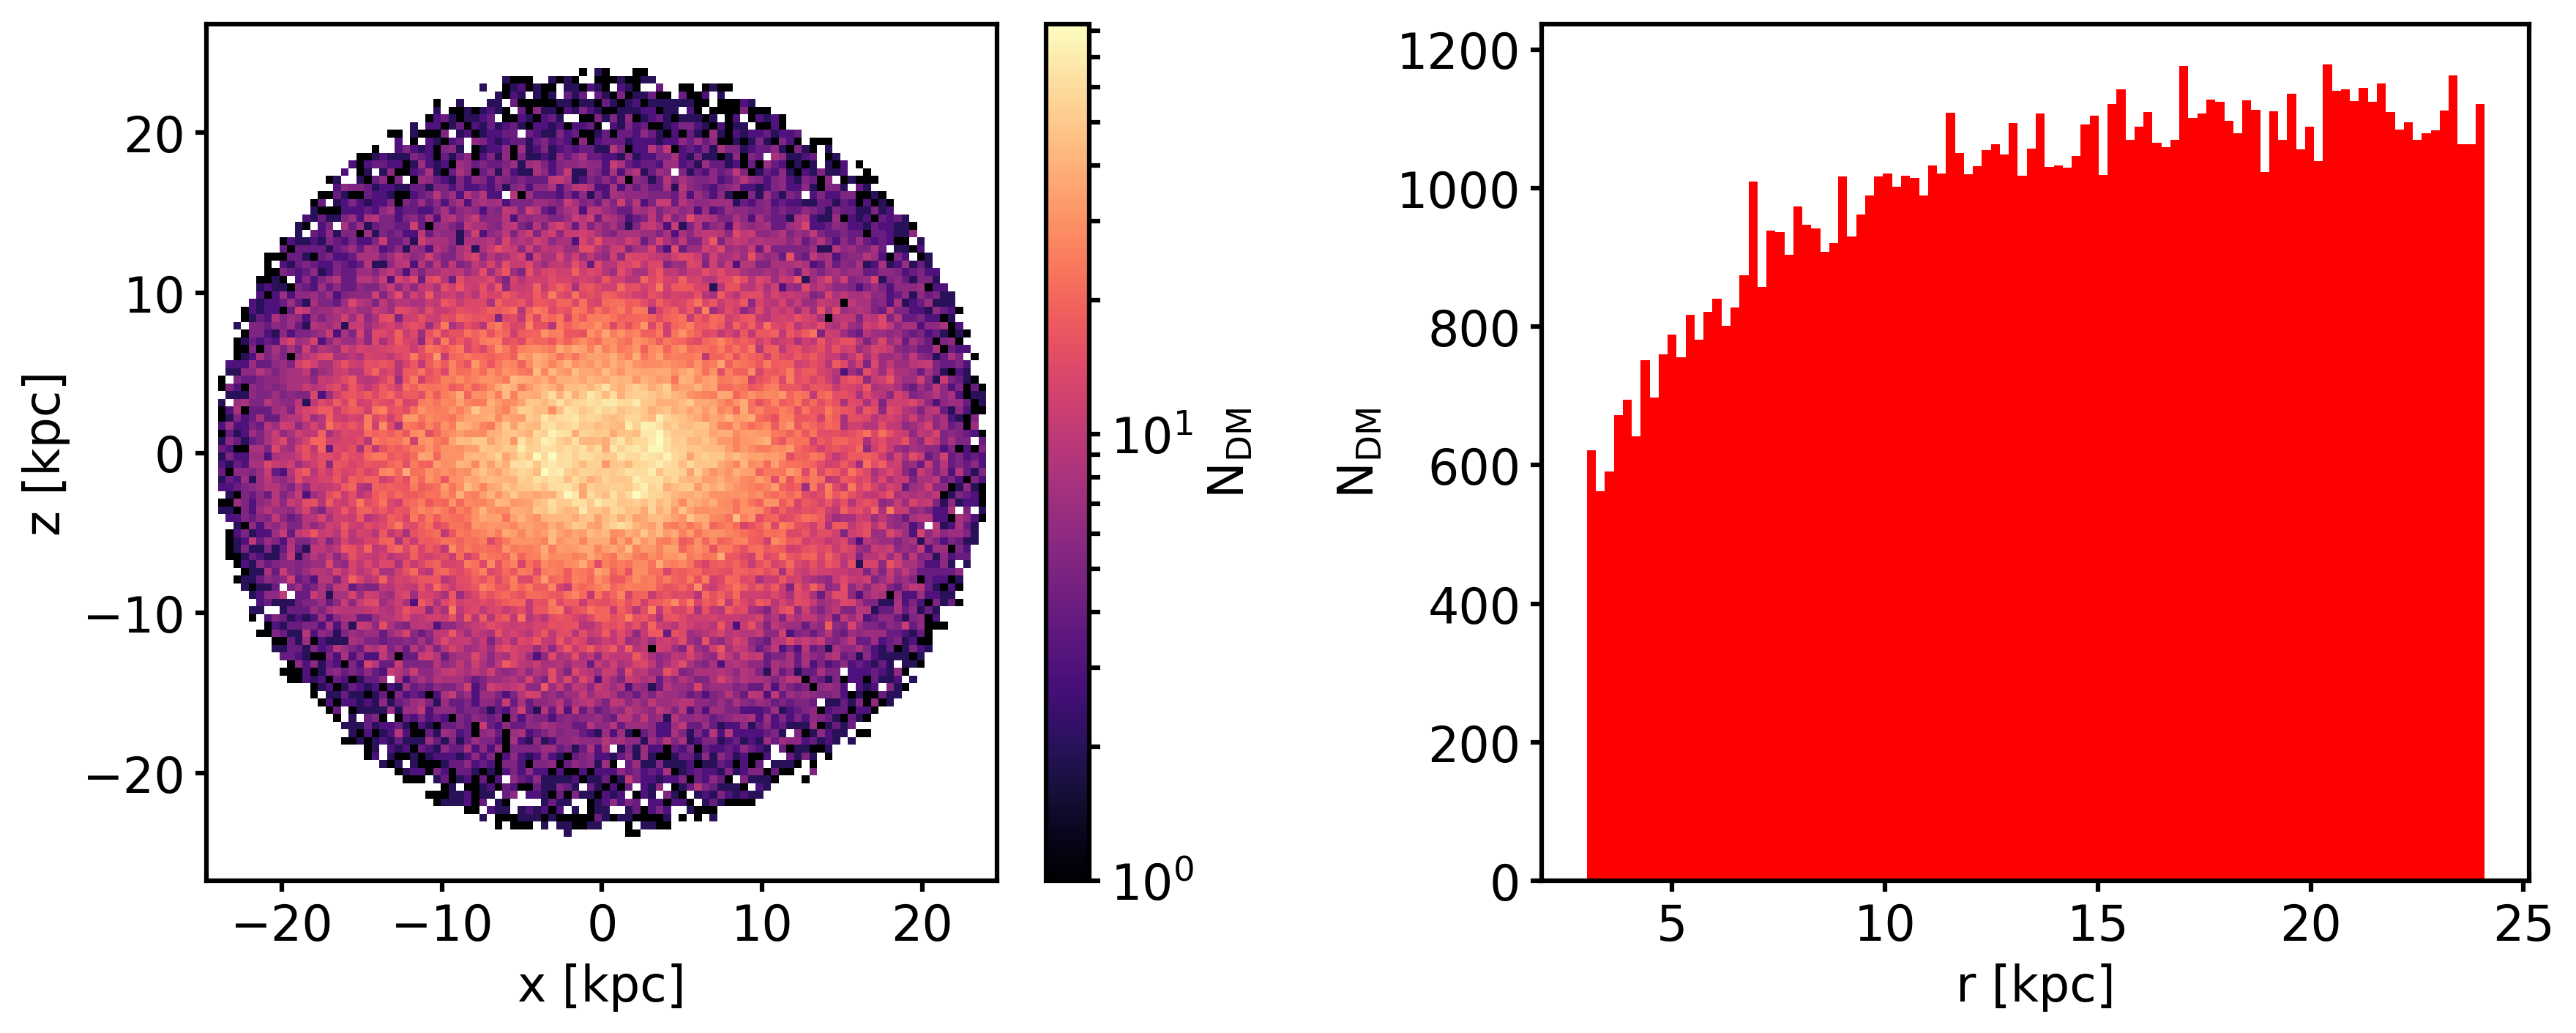
\includegraphics[width=\textwidth]{plots/Auriga/DM_selected_part_dist_snap_127.png}
    \caption{Selection of 100000 random \ac{DM} particles, used to fit to the \ac{NFW} halo. \textit{Left panel:} Distribution of particles in the x-z plane. \textit{Right panel:} Number of \ac{DM} particles depending on r. For radii > \SI{10}{kpc}, the distribution is constant while there are less particles for smaller radii. Since we are less interested in the innermost part of the halo, it is good that the weight for the fit lies in the outer parts. \ac{DM} particles with $r < \SI{3}{kpc}$ are excluded from the fit since it worsened the fit in the outer parts.}
    \label{fig:DM_part_selection}
\end{figure}
We select 100000 \ac{DM} particles randomly which we present in Figure \ref{fig:DM_part_selection}. With the best fit potentials for the stellar components, we set up a potential in galpy with all three components. We calculate the value of the potential for each of the randomly selected particles in the model and fit these to the true potential with the scipy.optimize.differential\_evolution routine by minimizing their squared relative errors.
\begin{SCfigure}
\captionsetup{format=plain}
    \centering
    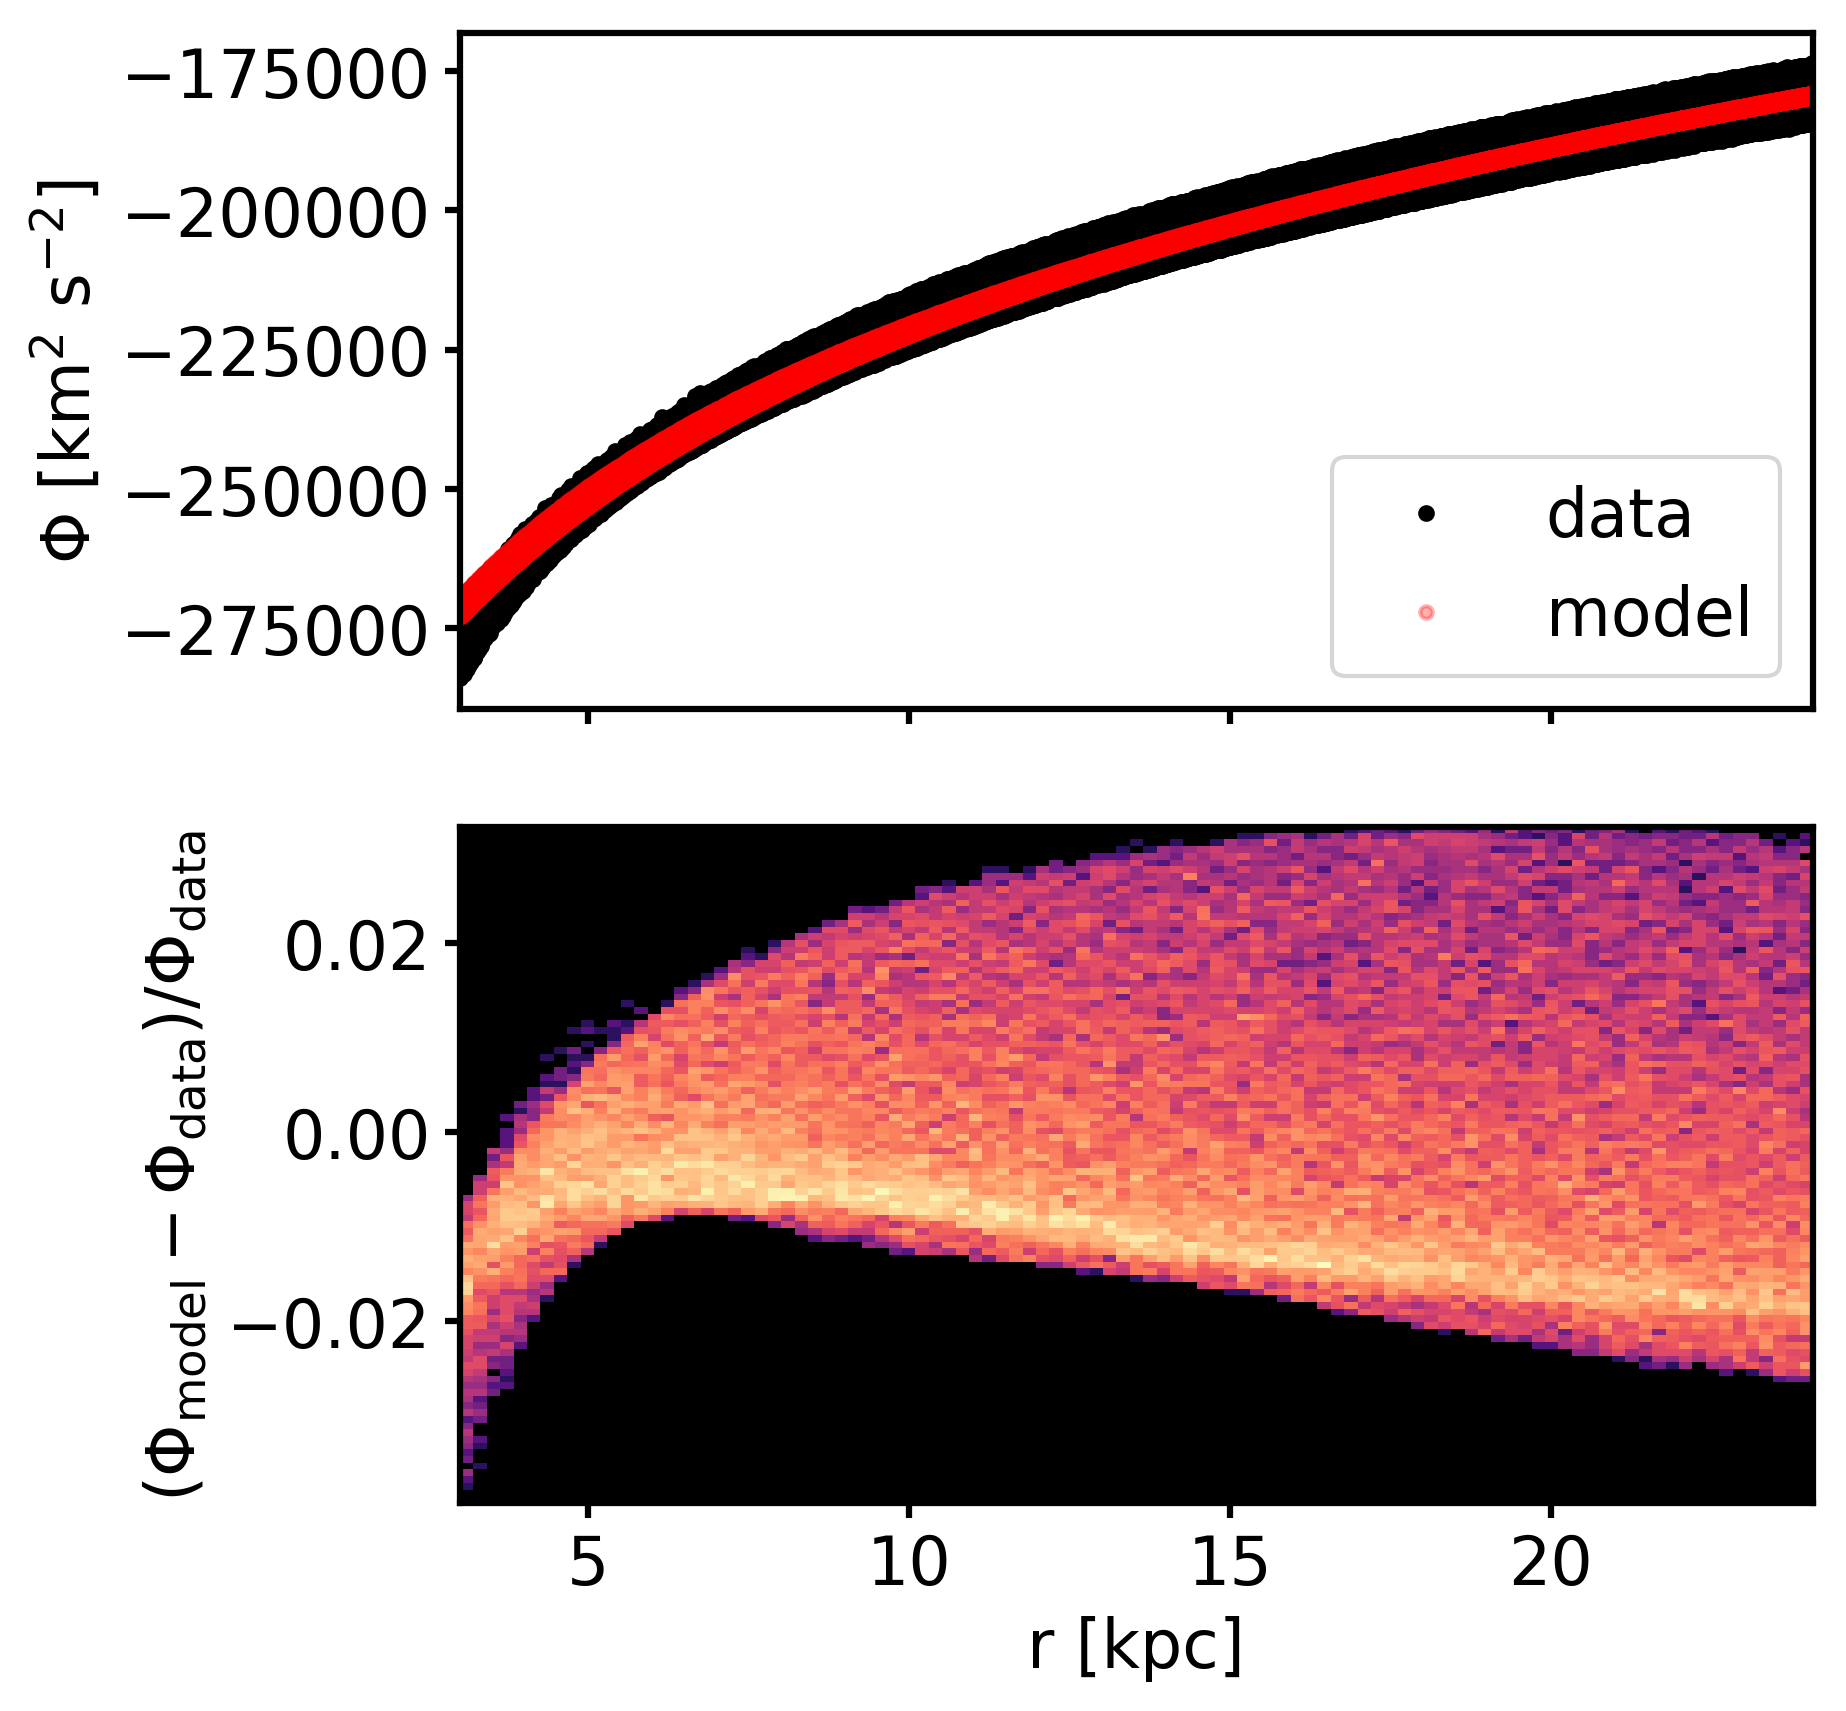
\includegraphics[width=0.7\textwidth]{plots/Auriga/phi_model_and_data_snap_with_rel_error_127.png}
    \caption{Potential of data (selected \ac{DM} particles) and model depending on the radius r. Black dots are data, red dots from the best fit model. The innermost \SI{3}{kpc} are not included in the fit to make it better in the outer parts. The model lies everywhere within the data range but the slope seems less steep than the slope of the data. The relative error is within a good range (<4\%).}
    \label{fig:potential_best_fit}
\end{SCfigure}
The result is shown in Figure \ref{fig:potential_best_fit} where we see the 'pot' value of the selected \ac{DM} particles in black and the fitted \ac{NFW} potential overlaying in red. Even though the red dots lie within the distribution of the black dots, the slope seems to be different. We find the best fit scale length of the \ac{DM} halo, $a_{\mathrm{NFWH}}$ as well as the total circular velocity $v_{0,\mathrm{tot}} \equiv v_{\mathrm{circ}}(R_0 = \SI{8}{kpc}) $. From that total circular velocity we can subtract the fraction from the stellar components to get the \ac{DM} component, $v_{0,\mathrm{NFWH}} = \sqrt{v_{0,\mathrm{tot}}^2 - v_{0, \mathrm{MND}}^2 - v_{0, \mathrm{HB}}^2}$. The resulting parameter values are summarized in Table \ref{tab:pot_best_fit_params}. 

\begin{figure}
\captionsetup{format=plain}
    \centering
    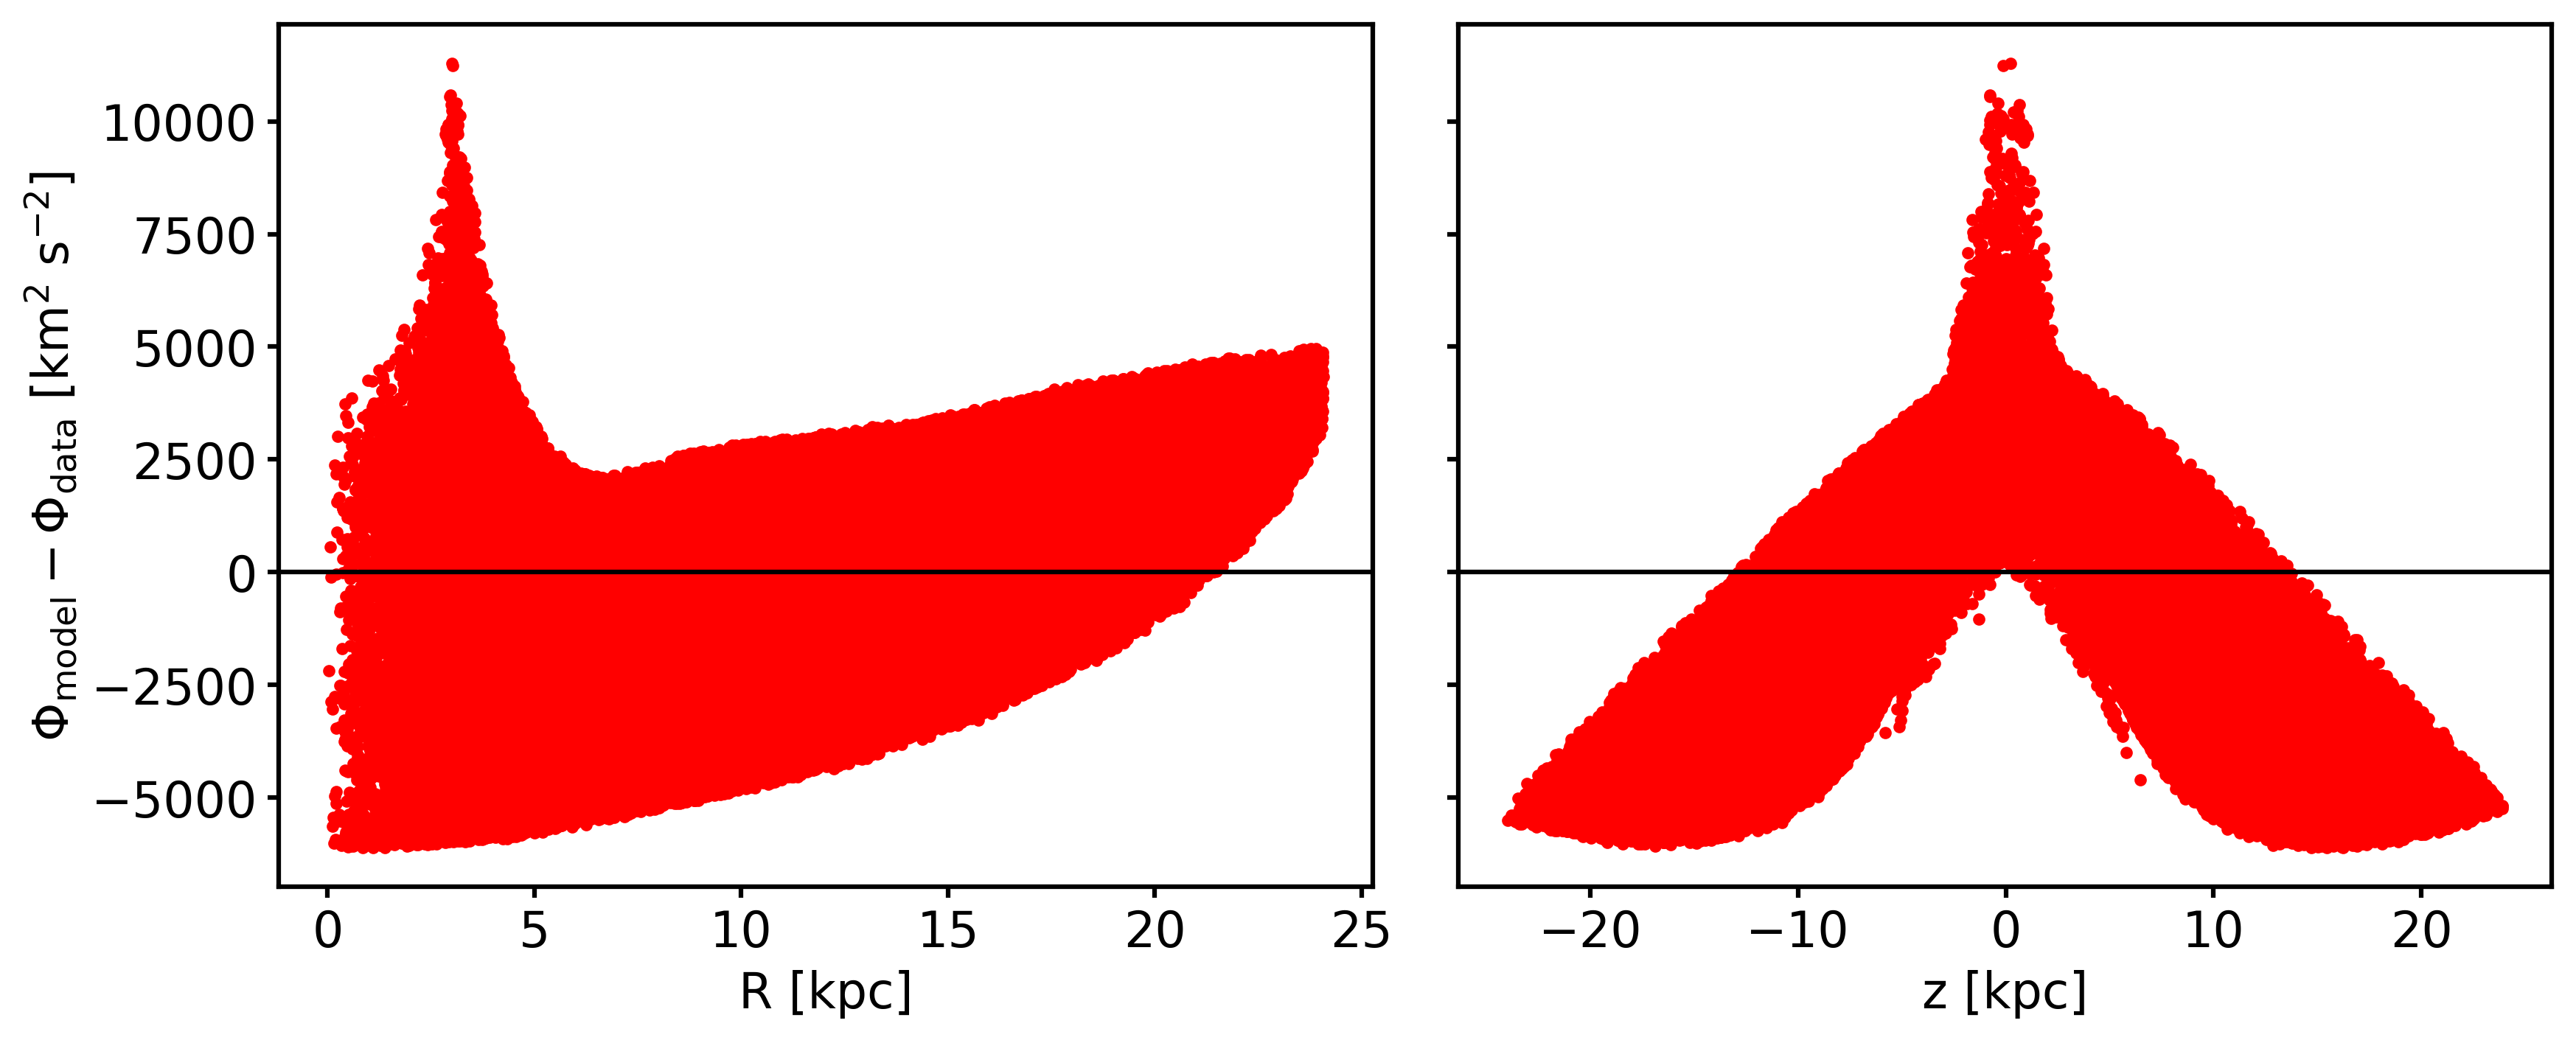
\includegraphics[width=\textwidth]{plots/Auriga/total_phi_error_snap_127.png}
    \caption{Total error $\Phi_\mathrm{model} - \Phi_\mathrm{data})$ of the \ac{DM} fit versus the three Radius an height $(R, z)$.}
    \label{fig:potential_fit_abs_errors}
\end{figure}
To check, how good the slope of the \ac{DM} fit is, we plot the relative error $(\Phi_\mathrm{model} - \Phi_\mathrm{data})/\Phi_\mathrm{data})$ versus the three cylindrical coordinates $(R, \phi, z)$. The slopes should be constant which they are not. We tried many different routines for the potential fit and this is the best we got and since the errors are relatively small (within 3-4\%) we still think the fit is good enough.

\subsubsection{Total potential}\label{subsubsec:tot_pot}
After fitting each component individually, we add them up to get a total potential.
\begin{table}[htbp]
\captionsetup{format=plain}
    \centering
    \begin{tabular}{@{}llll@{}}
         \toprule
         component& potential & parameters \& values &fitting method  \\
         \midrule
         stellar disk& \makecell[tl]{Miyamoto\\-Nagai}&\makecell[tl]{$a_{\mathrm{MND}}$ = \SI{2.97}{kpc}\\$b_{\mathrm{MND}}$ = \SI{1.64}{kpc}\\$v_{0,\mathrm{MND}}$ = \SI{105.00}{km.s^{-1}}} & \makecell[tl]{\ac{MN} density fitted \\to density bins \\of disk in $(R,z)$.}\vspace{3mm}\\
         %\midrule
         \makecell[tl]{stellar\\ spheroid}& Hernquist&\makecell[tl]{$a_{\mathrm{HB}}$ = \SI{1.82}{kpc}\\$v_{0,\mathrm{HB}}$ = \SI{110.00}{km.s^{-1}}}& \makecell[tl]{Hernquist density fitted\\ to density shells of \\spheroid in $(r)$.}\vspace{3mm}\\
         %\midrule
         \ac{DM} halo&\ac{NFW}&\makecell[tl]{$a_{\mathrm{NFWH}}$ = \SI{25.47}{kpc}\\$v_{0,\mathrm{NFWH}}$ = \SI{160.66}{km.s^{-1}}}&\makecell[tl]{Total potential fitted to \\'pot' value of random \ac{DM} \\particles where \ac{NFW}\\ parameters were fitting \\parameters.}\vspace{3mm}\\
         %\midrule
         total & \makecell[tl]{sum of these\\ potentials} & \makecell[tl]{$R_0$ = \SI{8.00}{kpc} \\ $v_{0,\mathrm{tot}}$ = \SI{221.21}{km.s^{-1}}}& \makecell[tl]{$v_0$ is the total circular \\ velocity at $R_0$.}\vspace{3mm}\\
         \bottomrule 
    \end{tabular}
    \caption{Best fit potential overview: components, used potentials, their parameters with best fit values and their fitting methods. \textcolor{red}{update absolute error and hist2d coming}}
    \label{tab:pot_best_fit_params}
\end{table}
In Table \ref{tab:pot_best_fit_params}, we summarize our results for the last snapshot as described in the previous Sections. 
 
\begin{table}[htbp]
\captionsetup{format=plain}
    \caption{Comparison of some of the structural parameters of our results with the Auriga \citep{AurigaGrand} analysis and \ac{MW} values taken from \citet{Bland-Hawthorn...MW...2016}.}
    \centering
    \begin{tabular}{@{}lllll@{}}
         \toprule
         Quantity & Unit& \makecell[tr]{This work} & \makecell[tr]{Auriga \\\citetalias{AurigaGrand} }&\makecell[tr]{Milky Way\\ \citetalias{Bland-Hawthorn...MW...2016}}\\
         \midrule
         \makecell[tl]{Disk scale length}& [kpc] & \makecell[tr]{2.97}&\makecell[tr]{5.57} & \makecell[tr]{$2.6\pm0.5$ \\(thin disk)}\\
         \makecell[tl]{Bulge scale length}& [kpc] & \makecell[tr]{1.82}&\makecell[tr]{0.95} & \makecell[tr]{$1.9-2.8$ \\\citetalias{Vanhollebeke...bulge...2009}}\\
         \makecell[tl]{\ac{DM} halo scale length}& [kpc] & \makecell[tr]{25.47}&\makecell[tr]{none} & \makecell[tr]{$25 \pm 10 $}\vspace{3mm}\\
         \makecell[tl]{Disk mass \\ within $0.1R_{200}$} & [$10^{10}\mathrm{M}_\odot$] &  \makecell[tr]{3.15}&\makecell[tr]{3.76} & \makecell[tr]{$3.5\pm1$\\(thin disk)}\\
         \makecell[tl]{Spheroid / bulge mass \\ within $0.1R_{200} $}& [$10^{10}\mathrm{M}_\odot$] &\makecell[tr]{3.40} &\makecell[tr]{2.19}& \makecell[tr]{$1.4-1.7$}\\
         \makecell[tl]{Total stellar mass \\ within $0.1R_{200}$ }& [$10^{10}\mathrm{M}_\odot$] & \makecell[tr]{6.55} &\makecell[tr]{6.55}& \makecell[tr]{$5 \pm 1$}\\
         \makecell[tl]{\ac{D/T}} & & \makecell[tr]{0.47}&\makecell[tr]{0.63} & \makecell[tr]{0.7 \\(thin disk)}\vspace{3mm}\\ 
         %\midrule
         \makecell[tl]{$R_{200}=R(\rho = 200 \rho_\mathrm{crit}$)} & [kpc] &\makecell[tr]{240.86}  & \makecell[tr]{240.86} & \makecell[tr]{$209 \pm 23$}\\
         \makecell[tl]{$M_{200}=M(\rho = 200 \rho_\mathrm{crit})$} & [$10^{12}\mathrm{M}_\odot$] & \makecell[tr]{149.18}  & \makecell[tr]{149.18} & \makecell[tr]{$1.1 \pm 0.3$}\vspace{3mm}\\
         %\midrule
         \makecell[tl]{total circular velocity\\ at $R_0 = \SI{8}{kpc}$}&  [$\mathrm{km\ s}^{-1}$]& \makecell[tr]{221.21} & \makecell[tr]{none \\explicitly}& \makecell[tr]{$238 \pm 15$}\vspace{3mm}\\
         \bottomrule 
    \end{tabular}

    \label{tab:disk_quant_comparison}
\end{table}




\iffalse
\begin{figure}
\captionsetup{format=plain}
    \centering
    \begin{subfigure}[b]{0.3\textwidth}
	    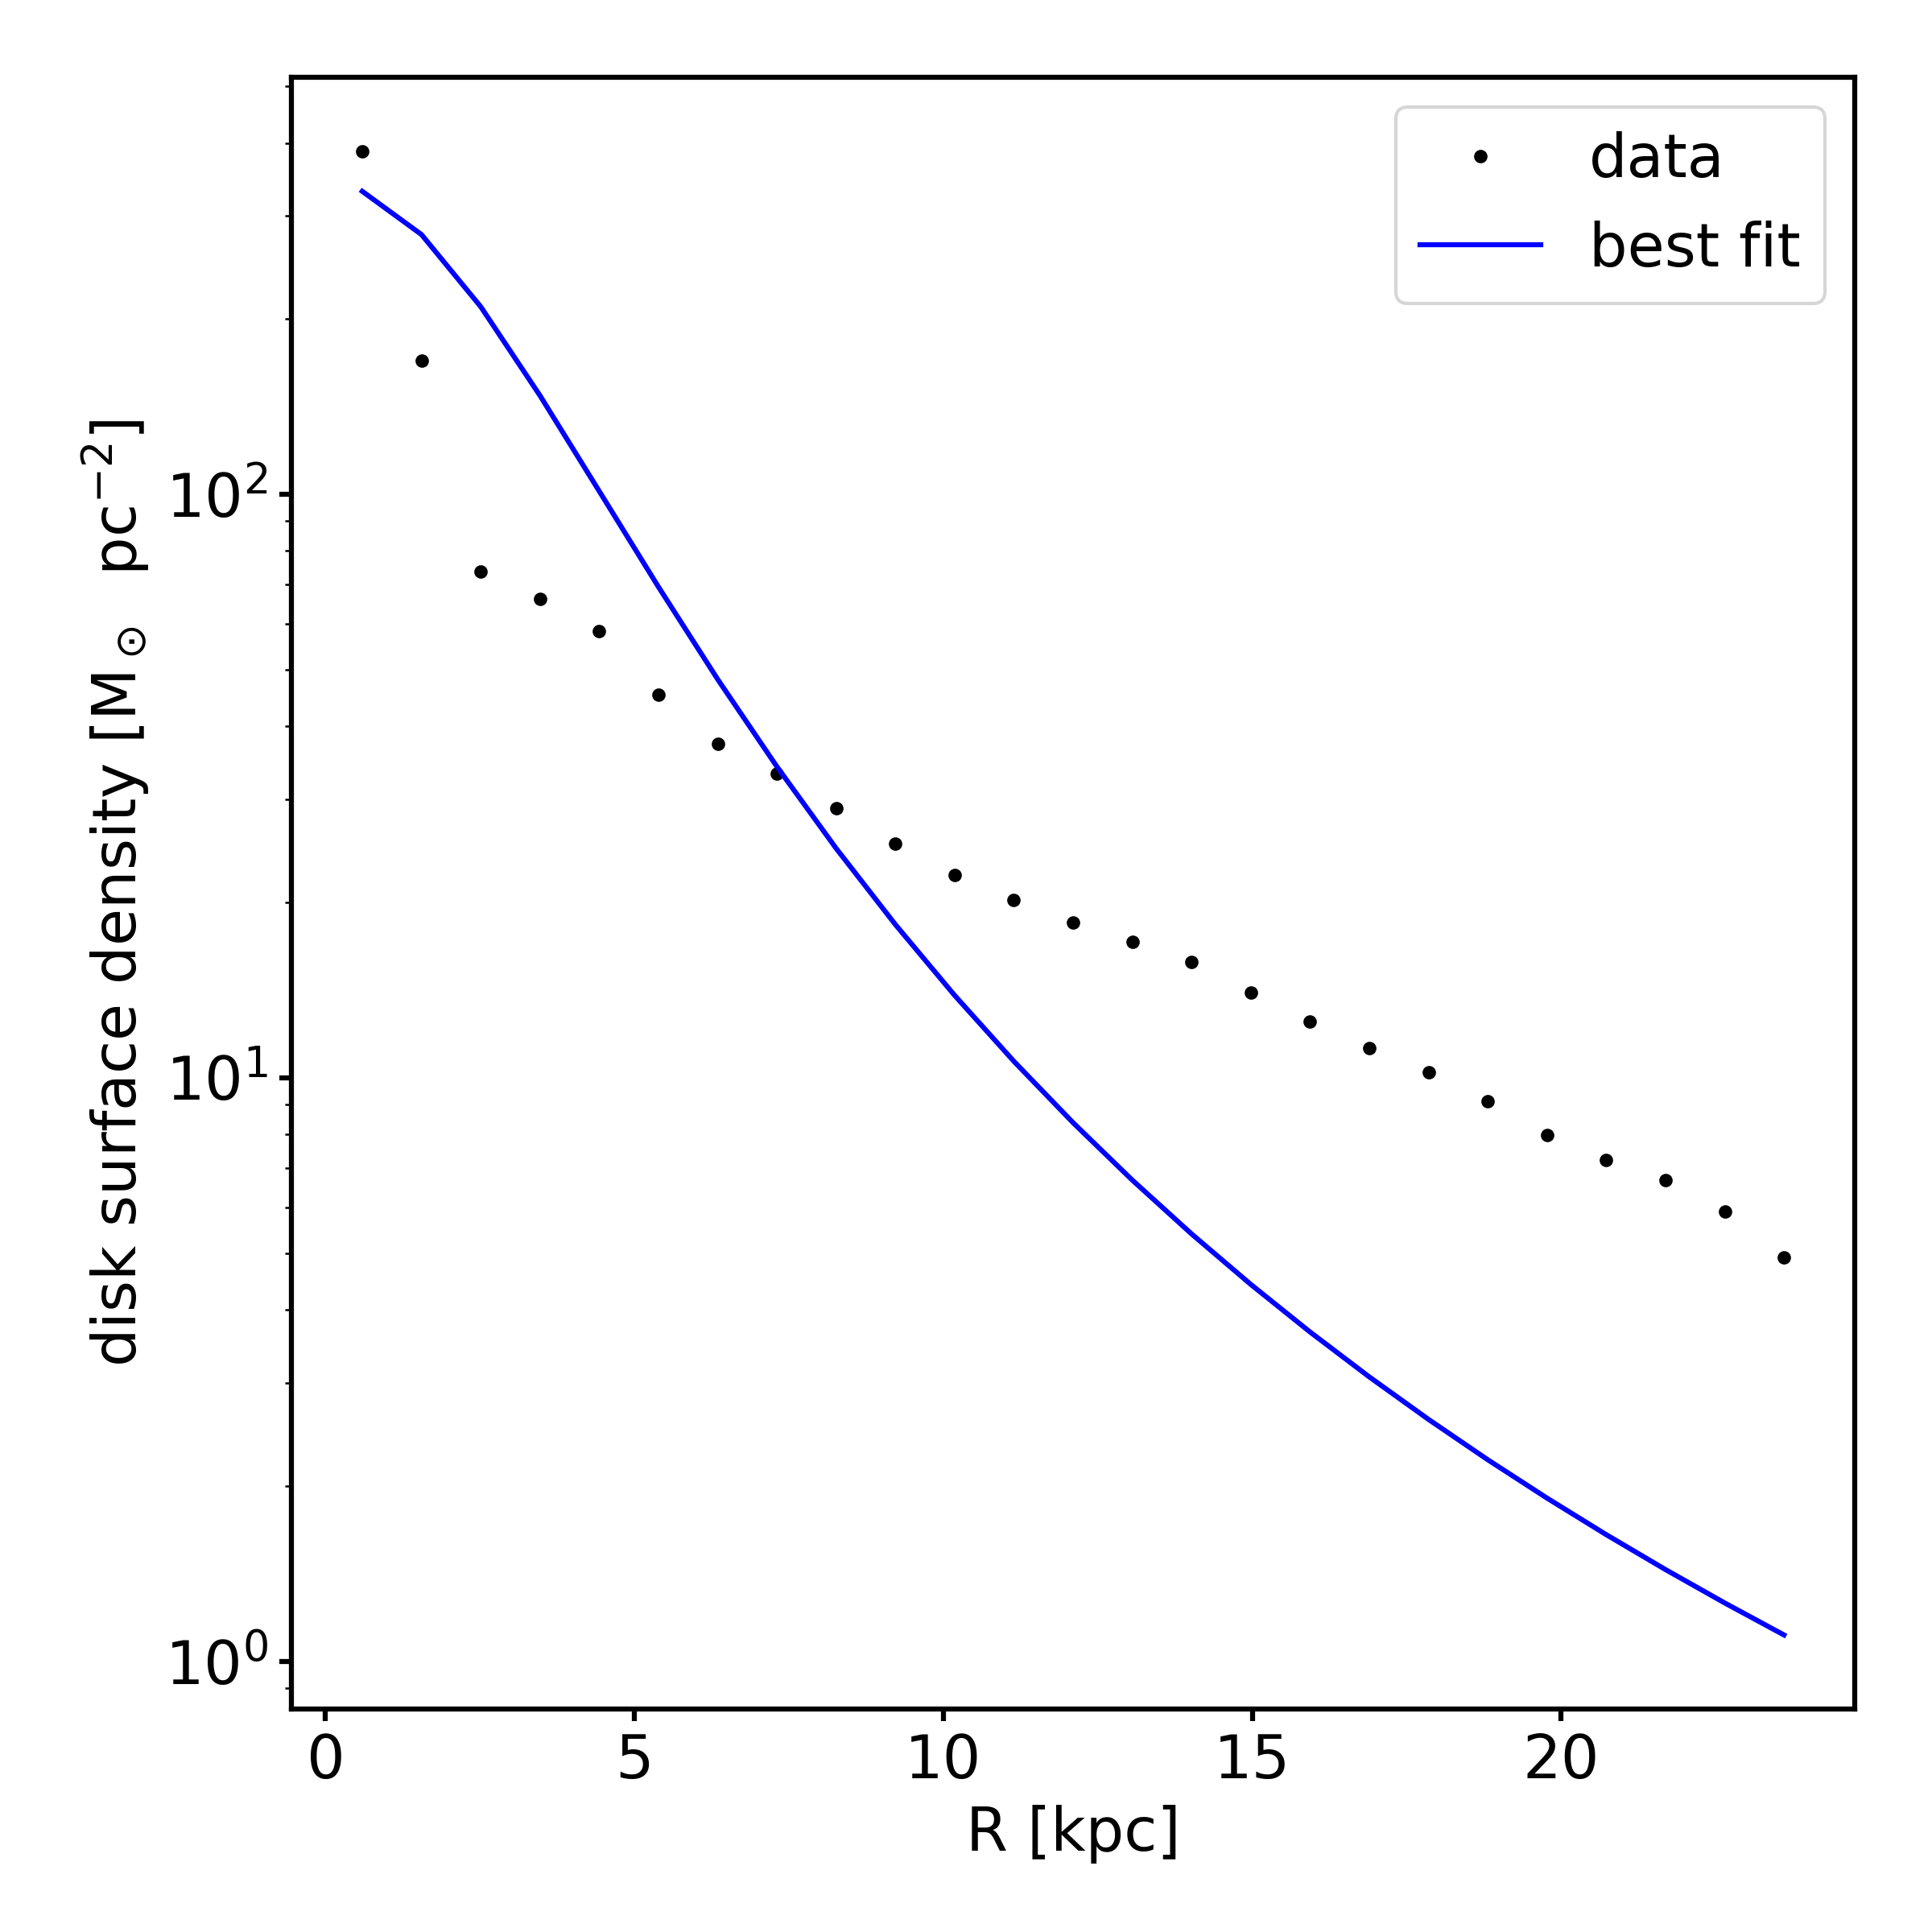
\includegraphics[width=\textwidth]{plots/Auriga/surface_dens_disk_fit_data.png}
	    \label{fig:disk_surfdens_fit}
    \end{subfigure}
    ~ %add desired spacing between images, e. g. ~, \quad, \qquad, \hfill etc. 
      %(or a blank line to force the subfigure onto a new line)
    \begin{subfigure}[b]{0.3\textwidth}
    \centering
    	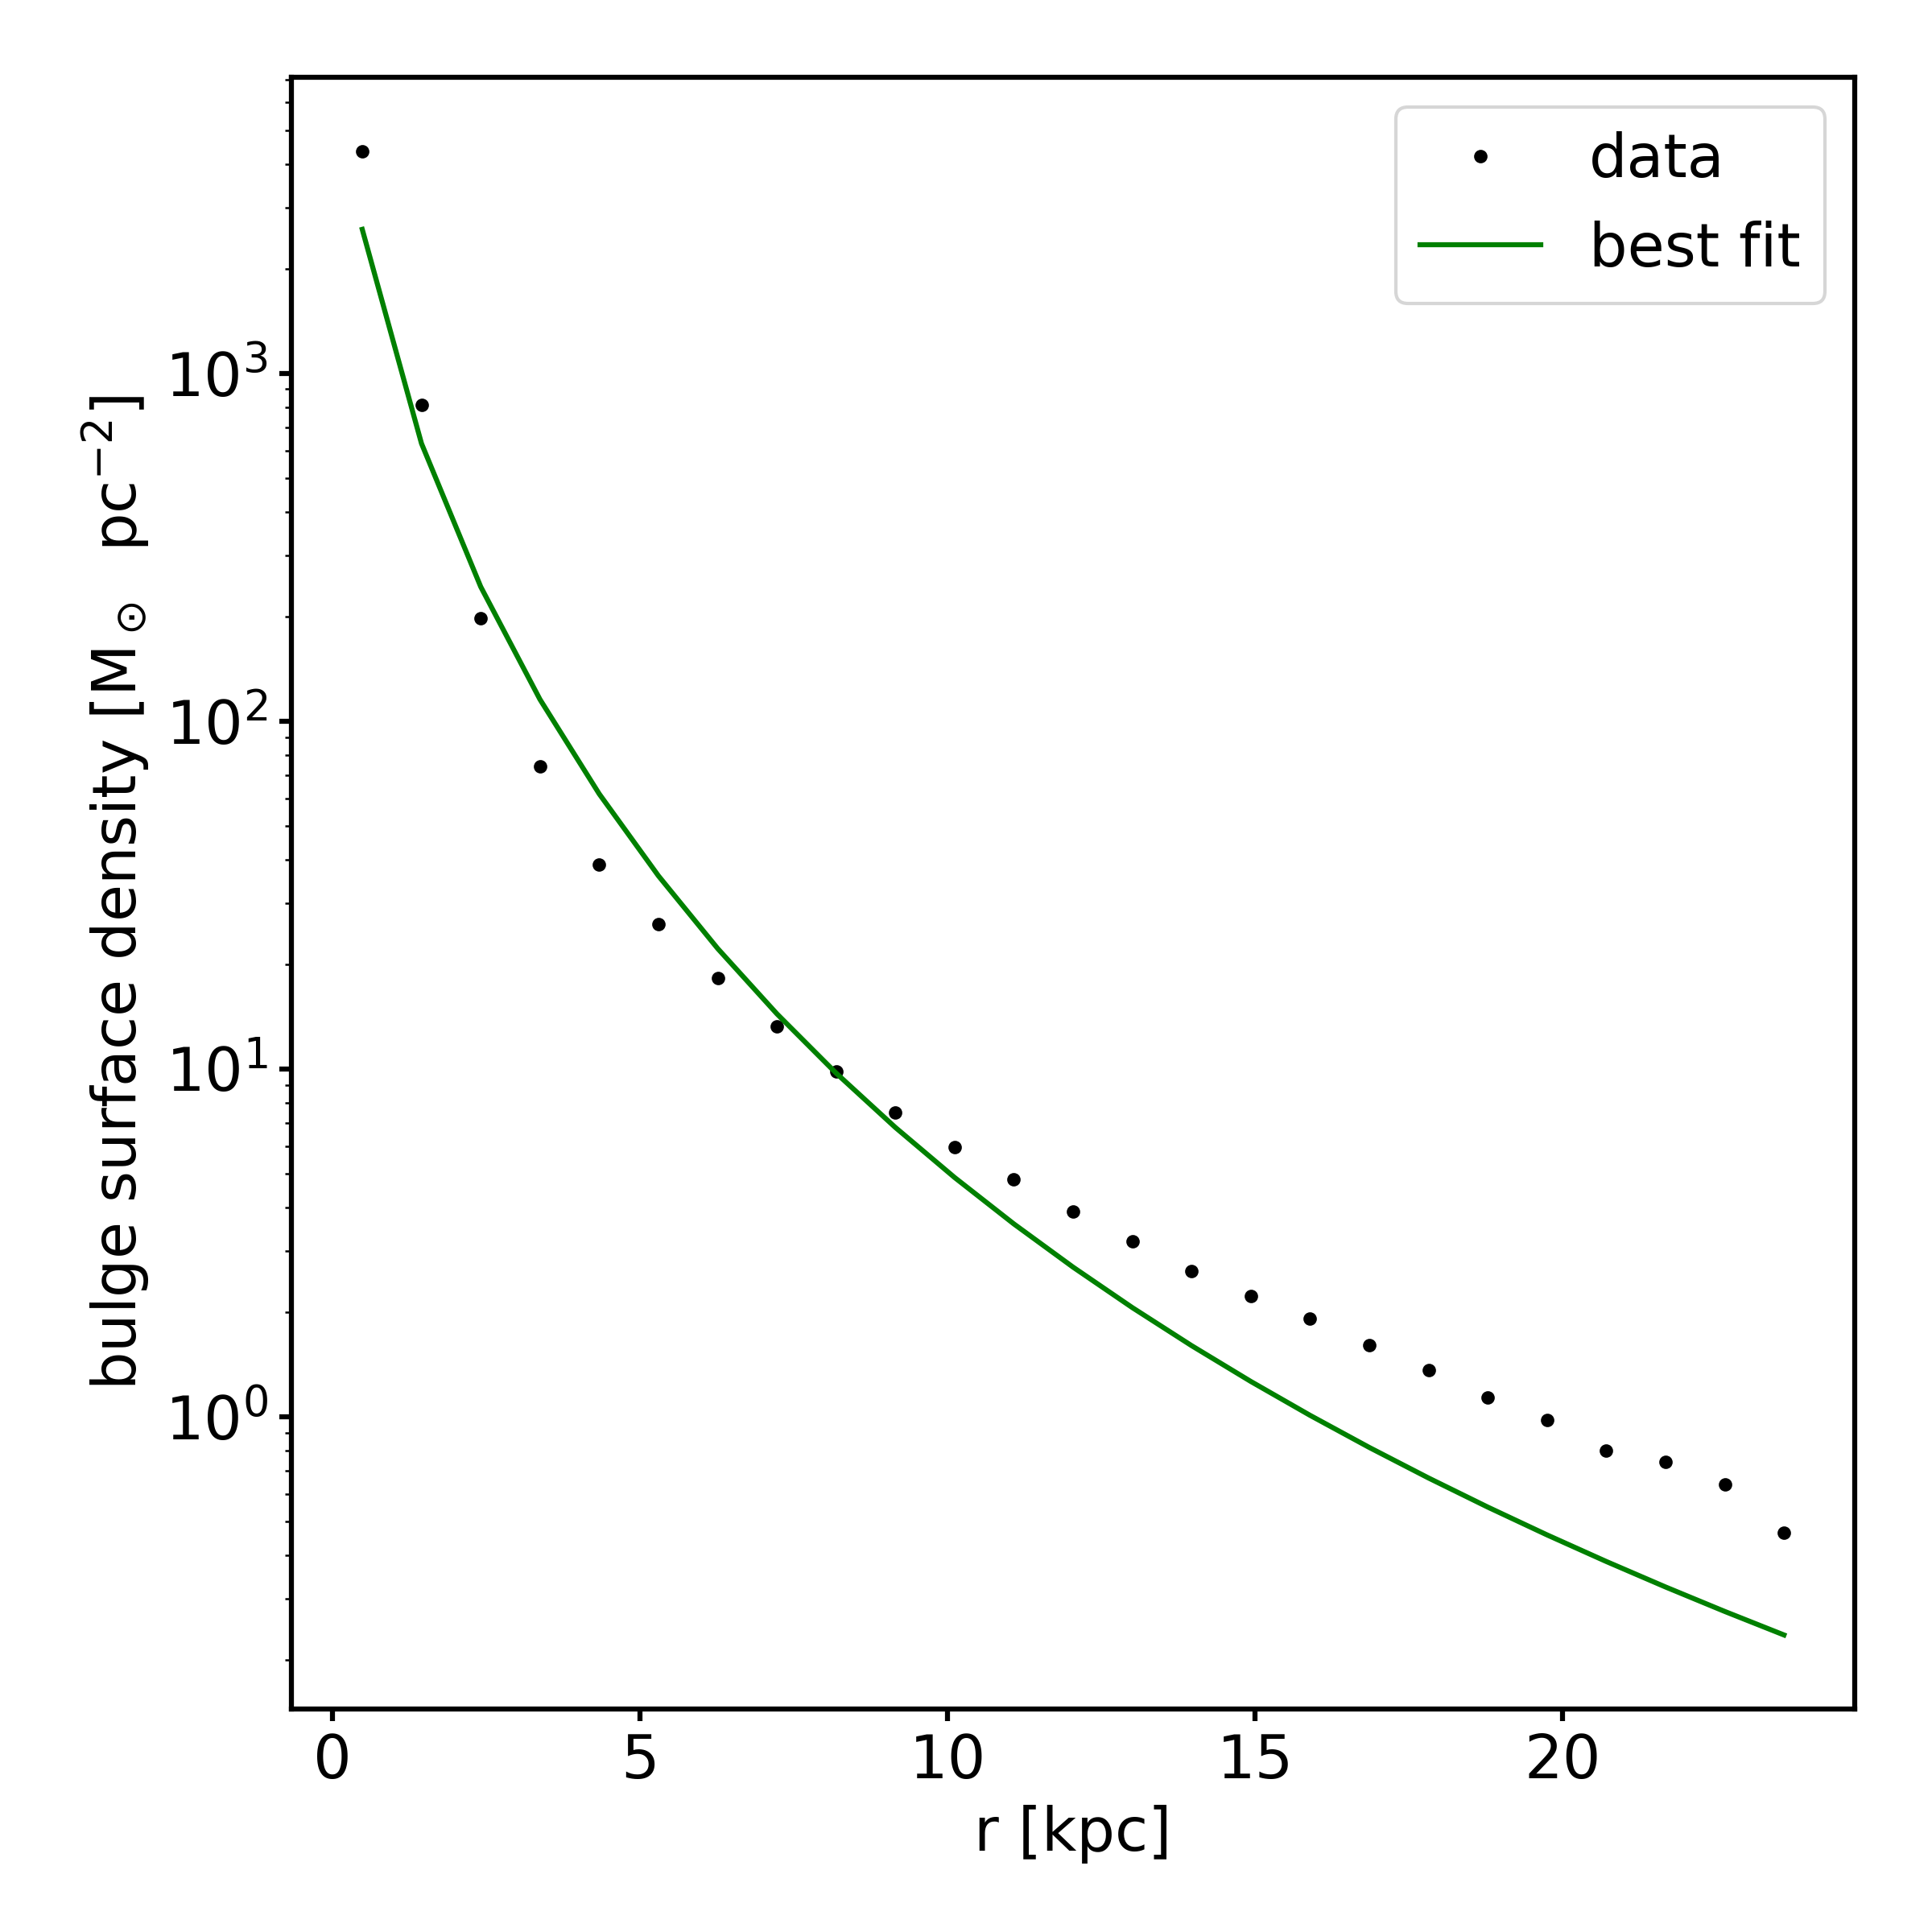
\includegraphics[width=\textwidth]{plots/Auriga/surface_dens_spher_fit_data.png}
    	\label{fig:spher_surfdens_fit}
    \end{subfigure}
    ~ %add desired spacing between images, e. g. ~, \quad, \qquad, \hfill etc. 
    %(or a blank line to force the subfigure onto a new line)
    \begin{subfigure}[b]{0.3\textwidth}
    \centering
    	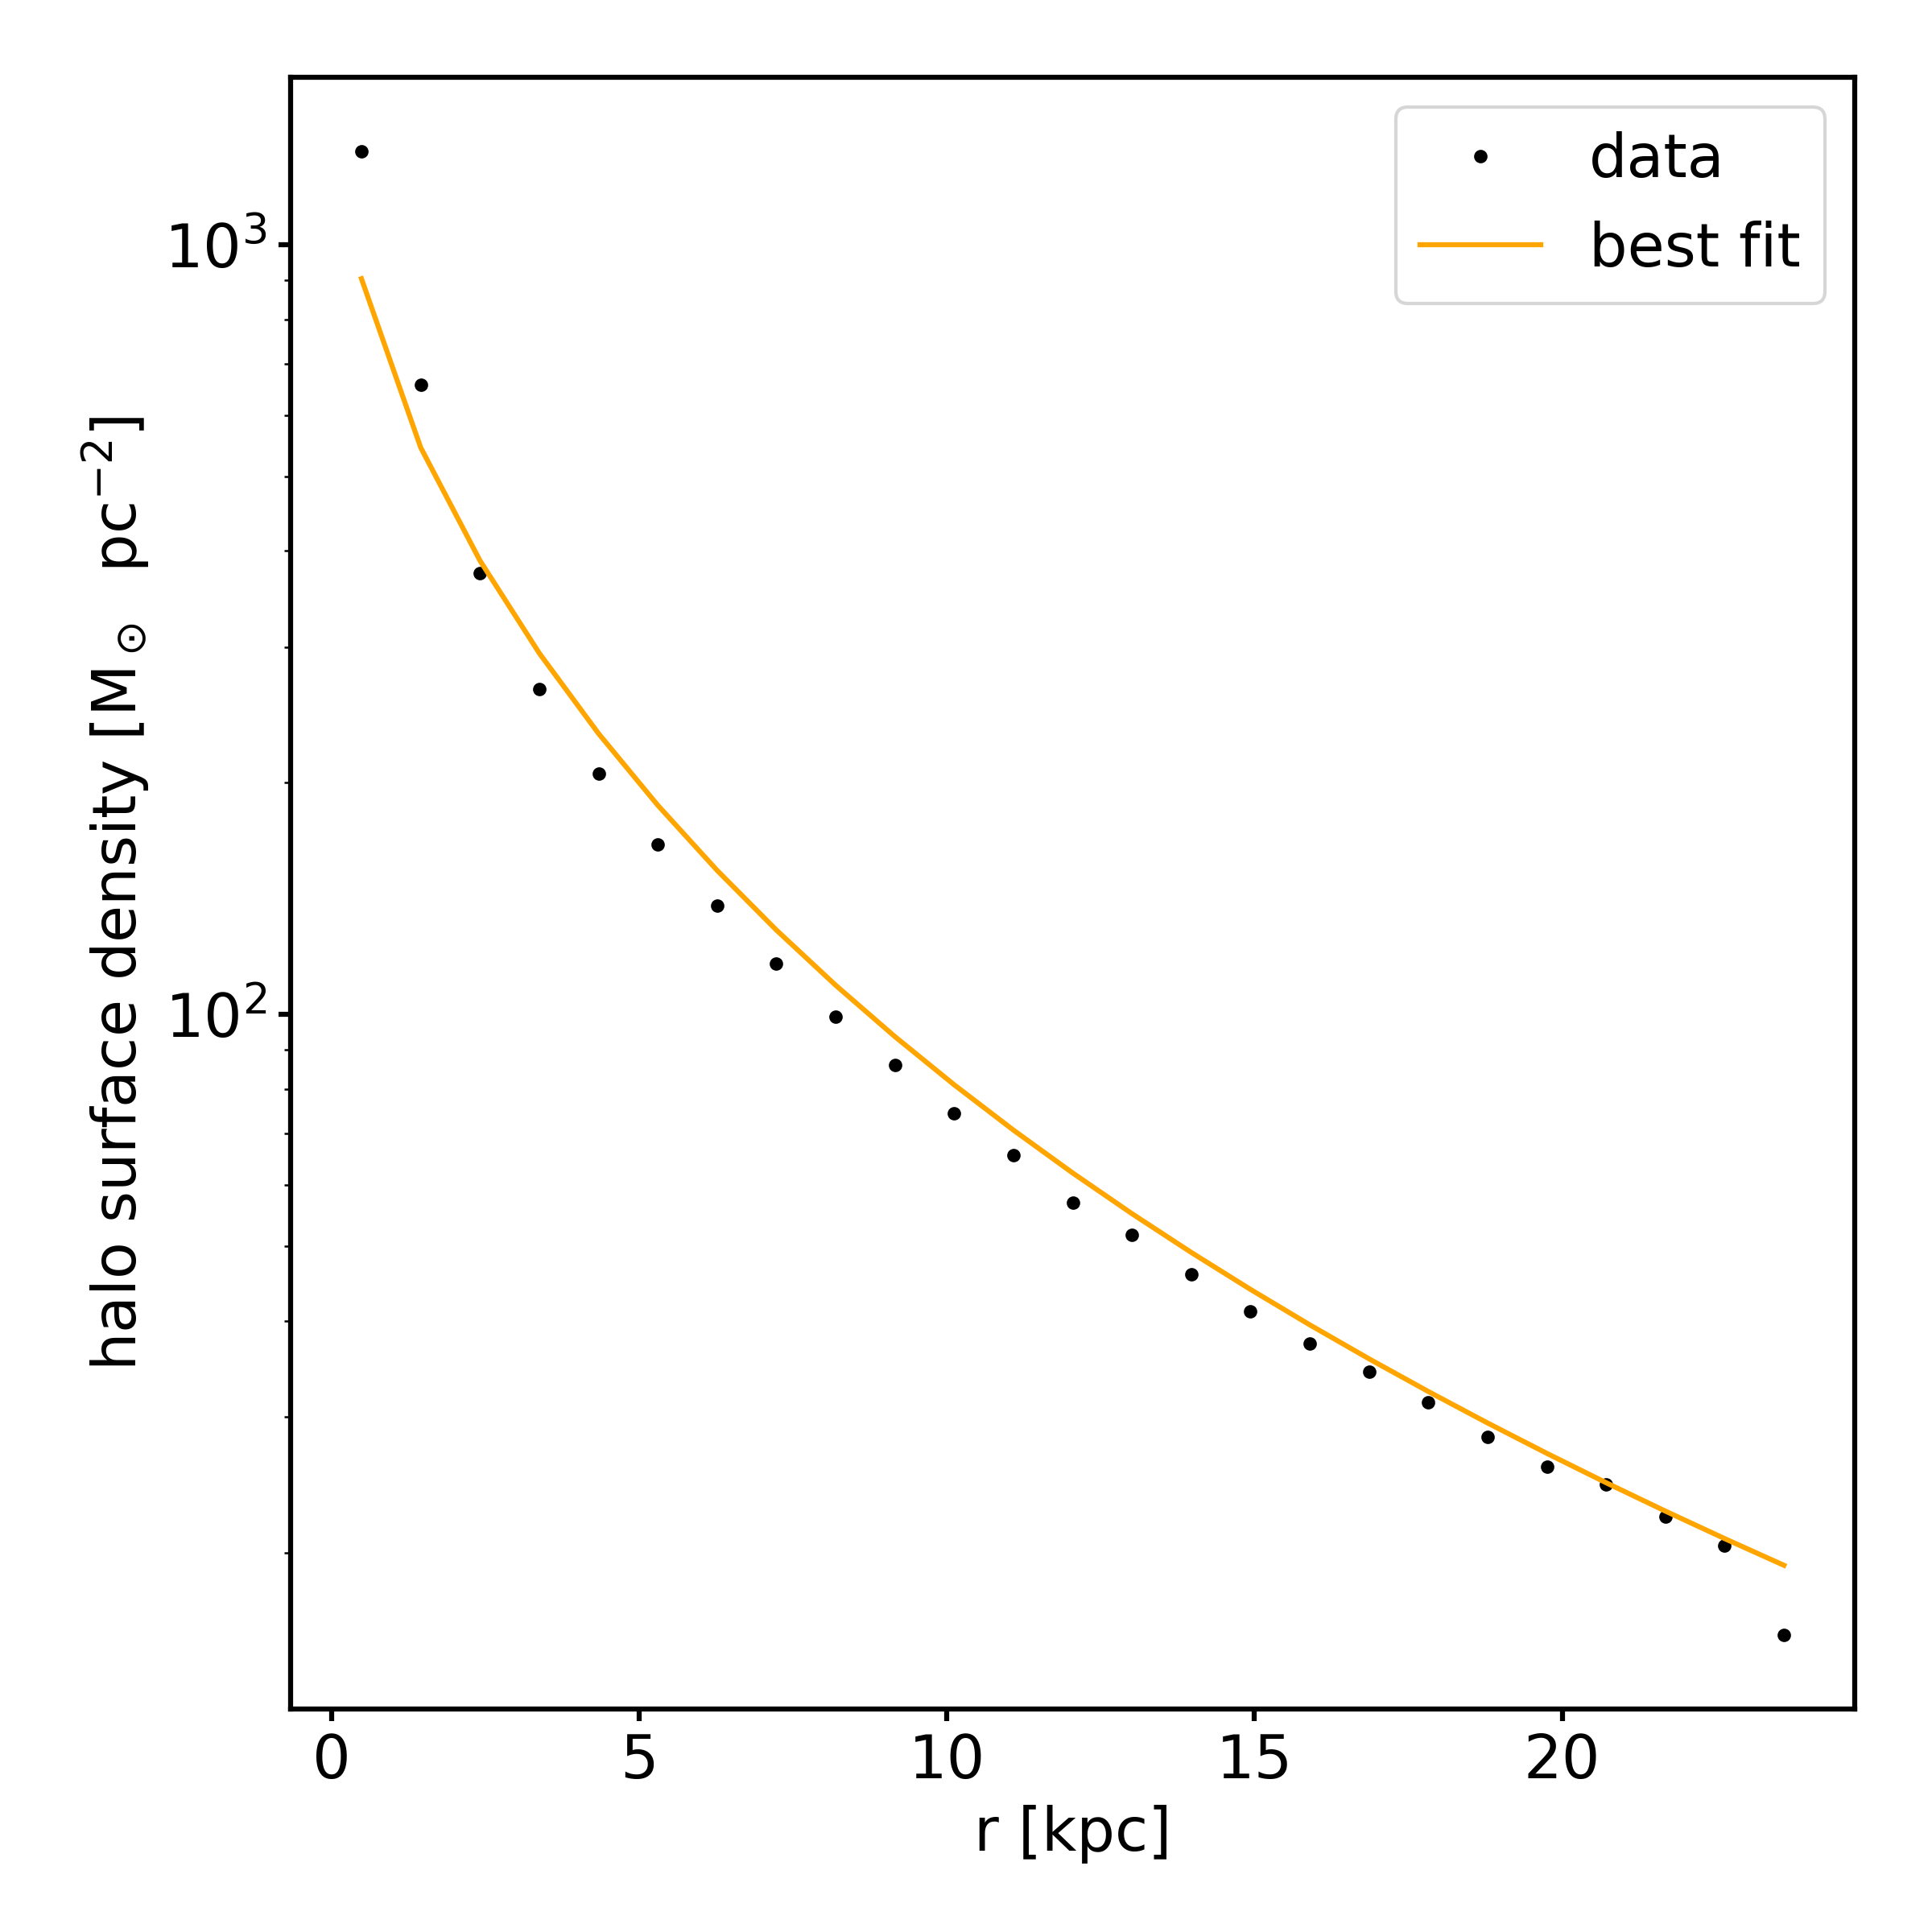
\includegraphics[width=\textwidth]{plots/Auriga/surface_dens_halo_fit_data.png}
    	\label{fig:halo_surfdens_fit}
    \end{subfigure}
    
    \begin{subfigure}[b]{0.3\textwidth}
        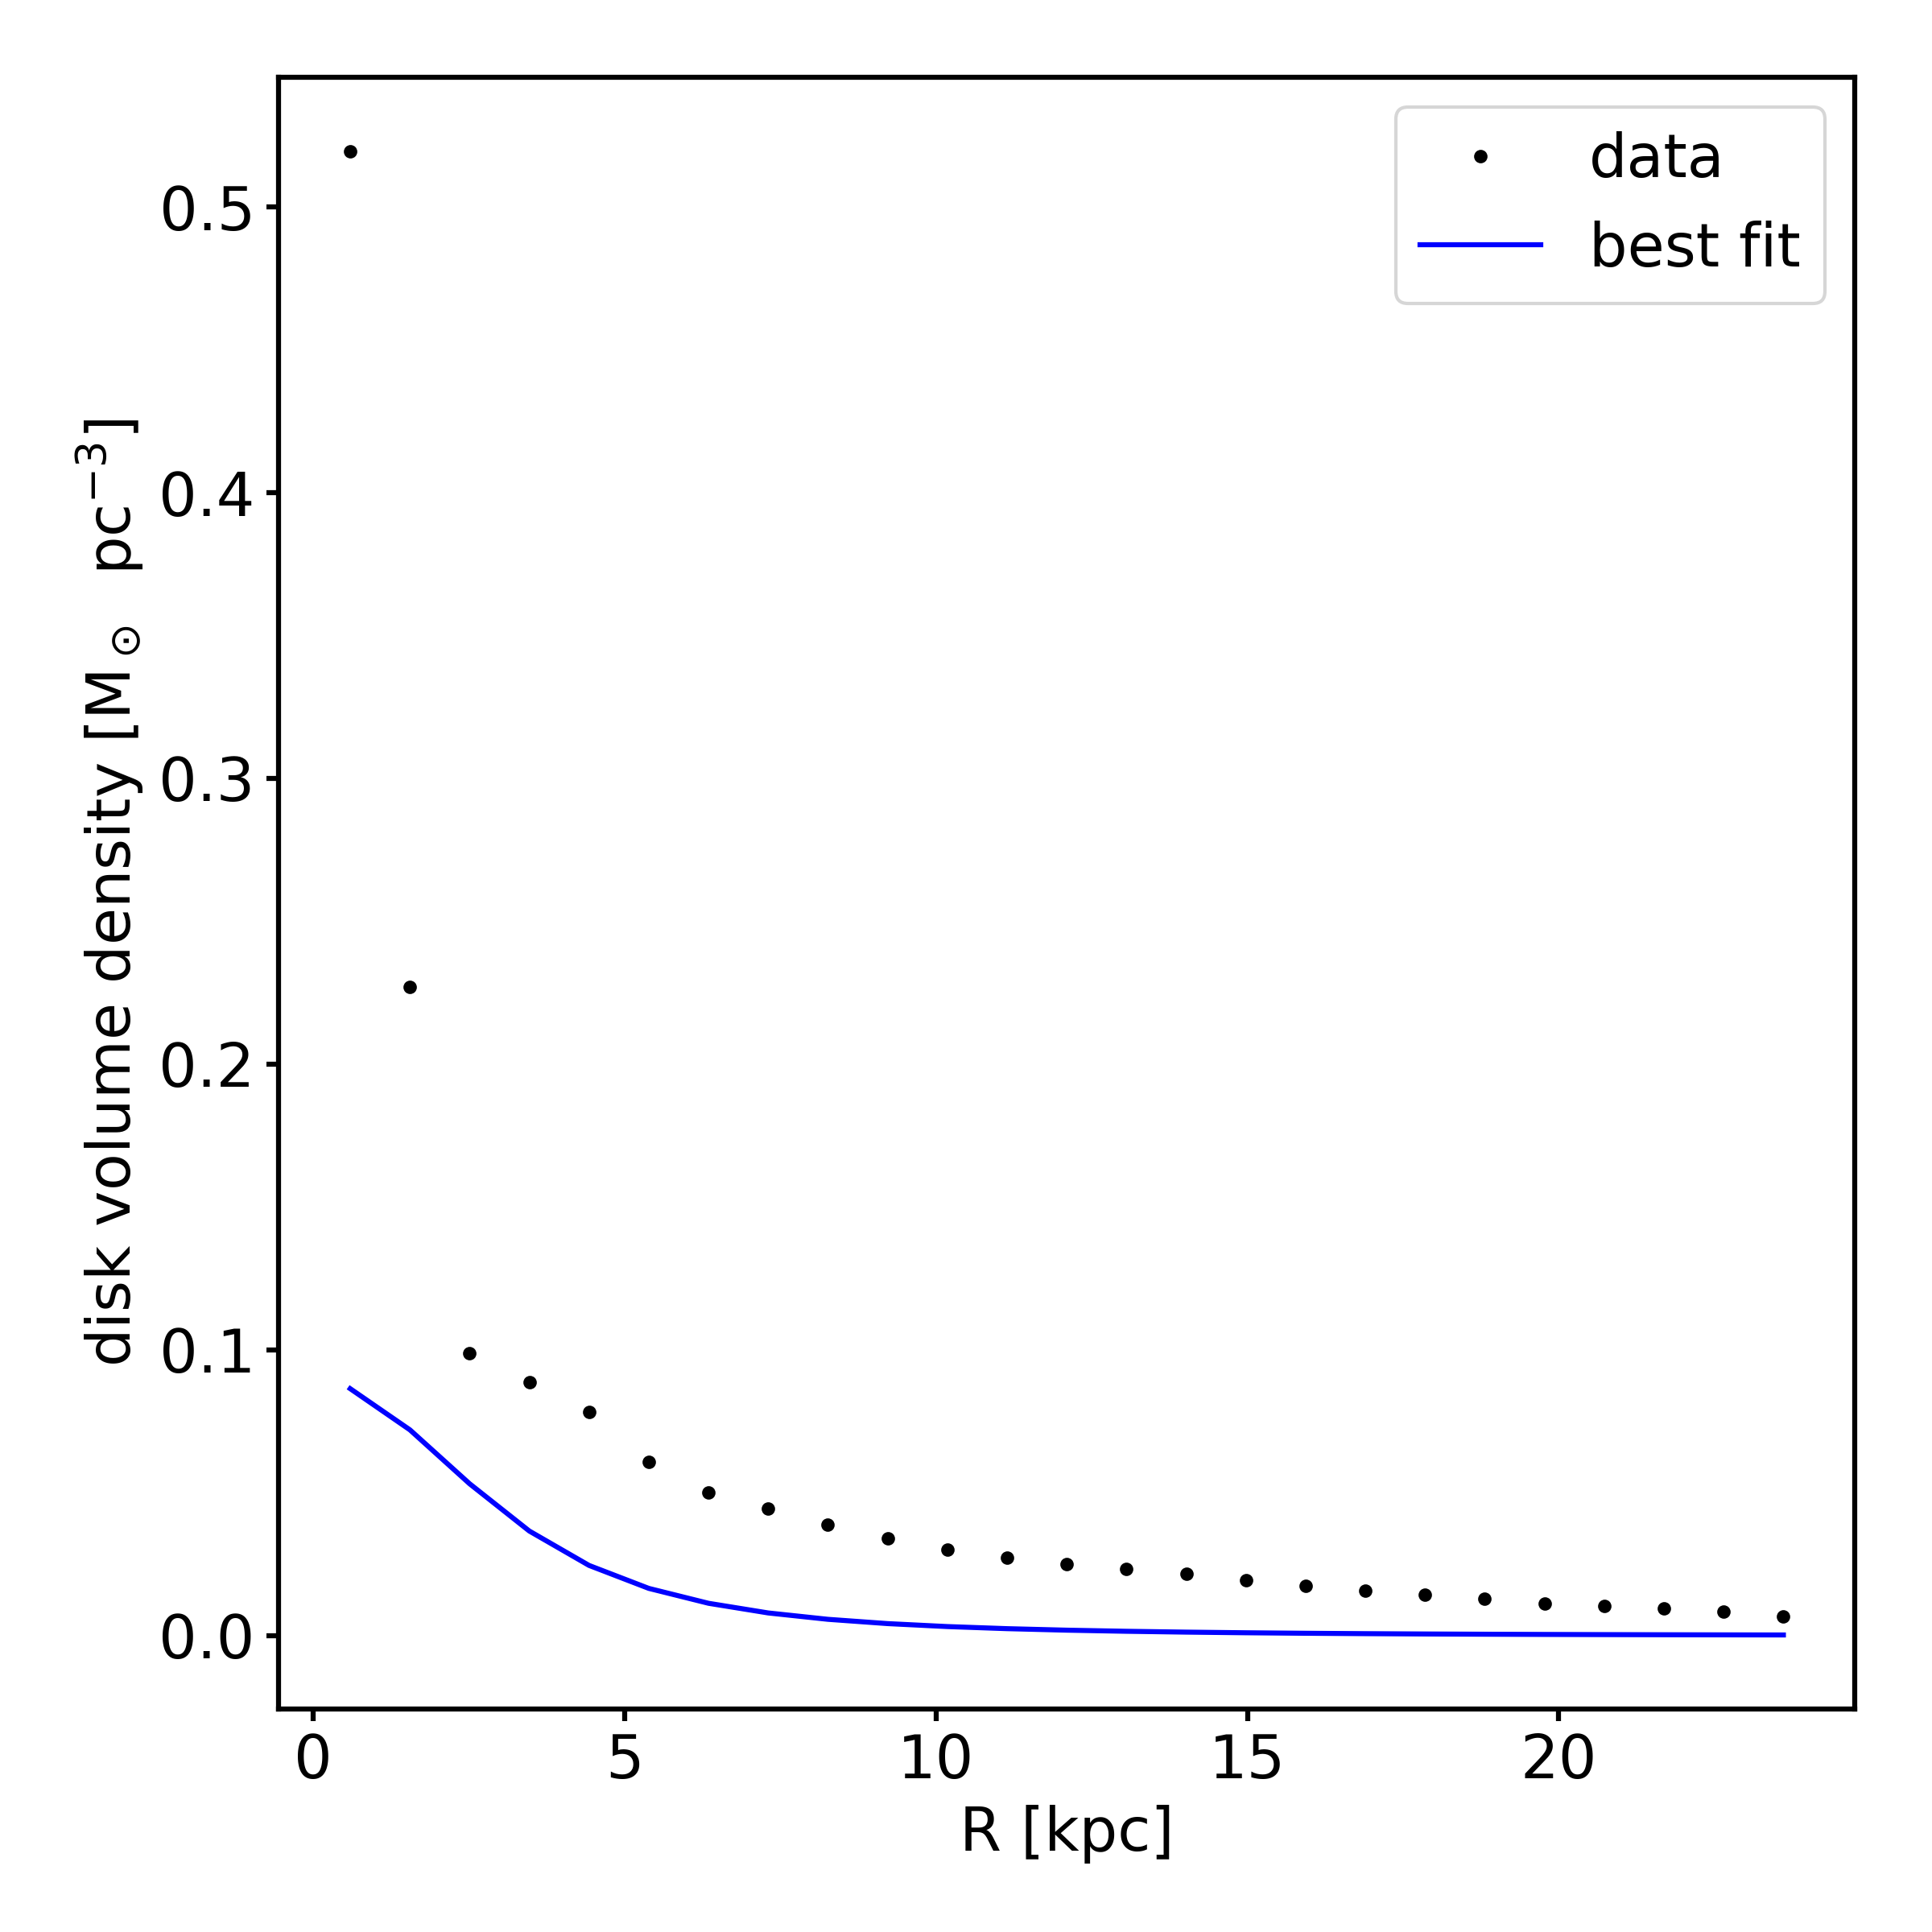
\includegraphics[width=\textwidth]{plots/Auriga/volume_dens_disk_fit_data.png}
	    \label{fig:disk_voldens_fit}
    \end{subfigure}
    ~ %add desired spacing between images, e. g. ~, \quad, \qquad, \hfill etc. 
    %(or a blank line to force the subfigure onto a new line)
    \begin{subfigure}[b]{0.3\textwidth}
    \centering
    	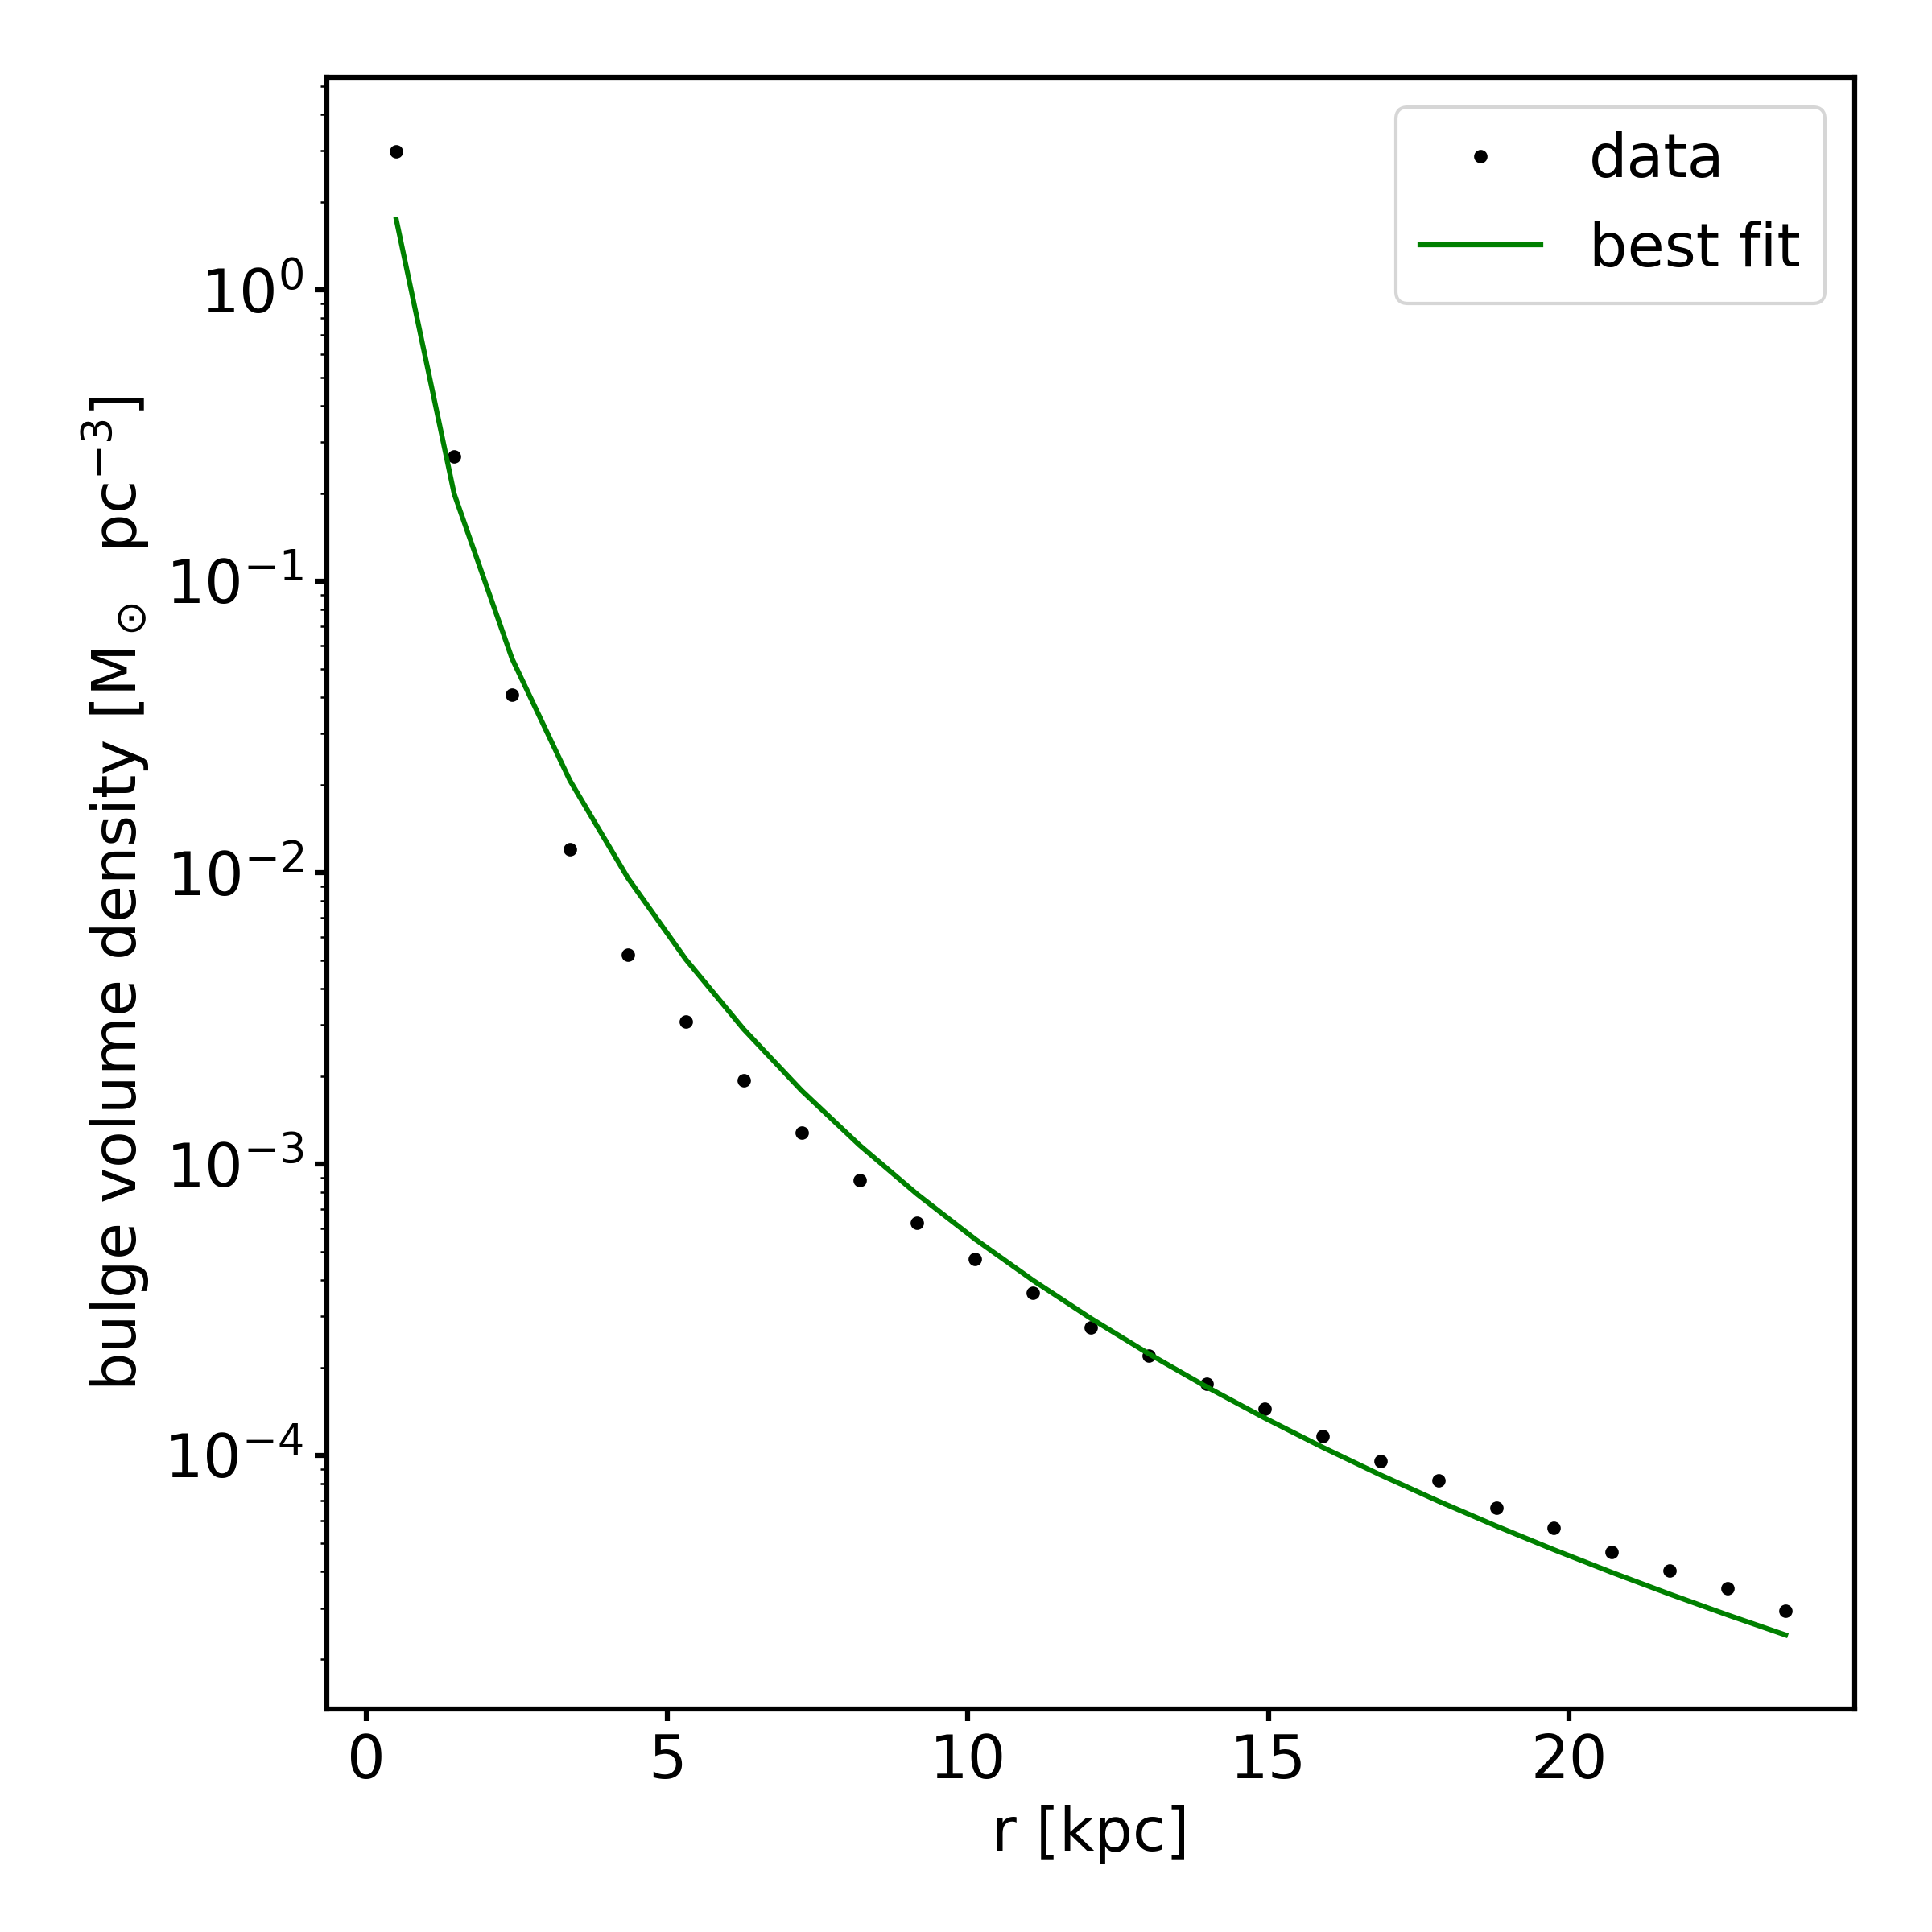
\includegraphics[width=\textwidth]{plots/Auriga/volume_dens_bulge_fit_data.png}
    	\label{fig:spher_voldens_fit}
    \end{subfigure}
    ~ %add desired spacing between images, e. g. ~, \quad, \qquad, \hfill etc. 
    %(or a blank line to force the subfigure onto a new line)
    \begin{subfigure}[b]{0.3\textwidth}
        \centering
    	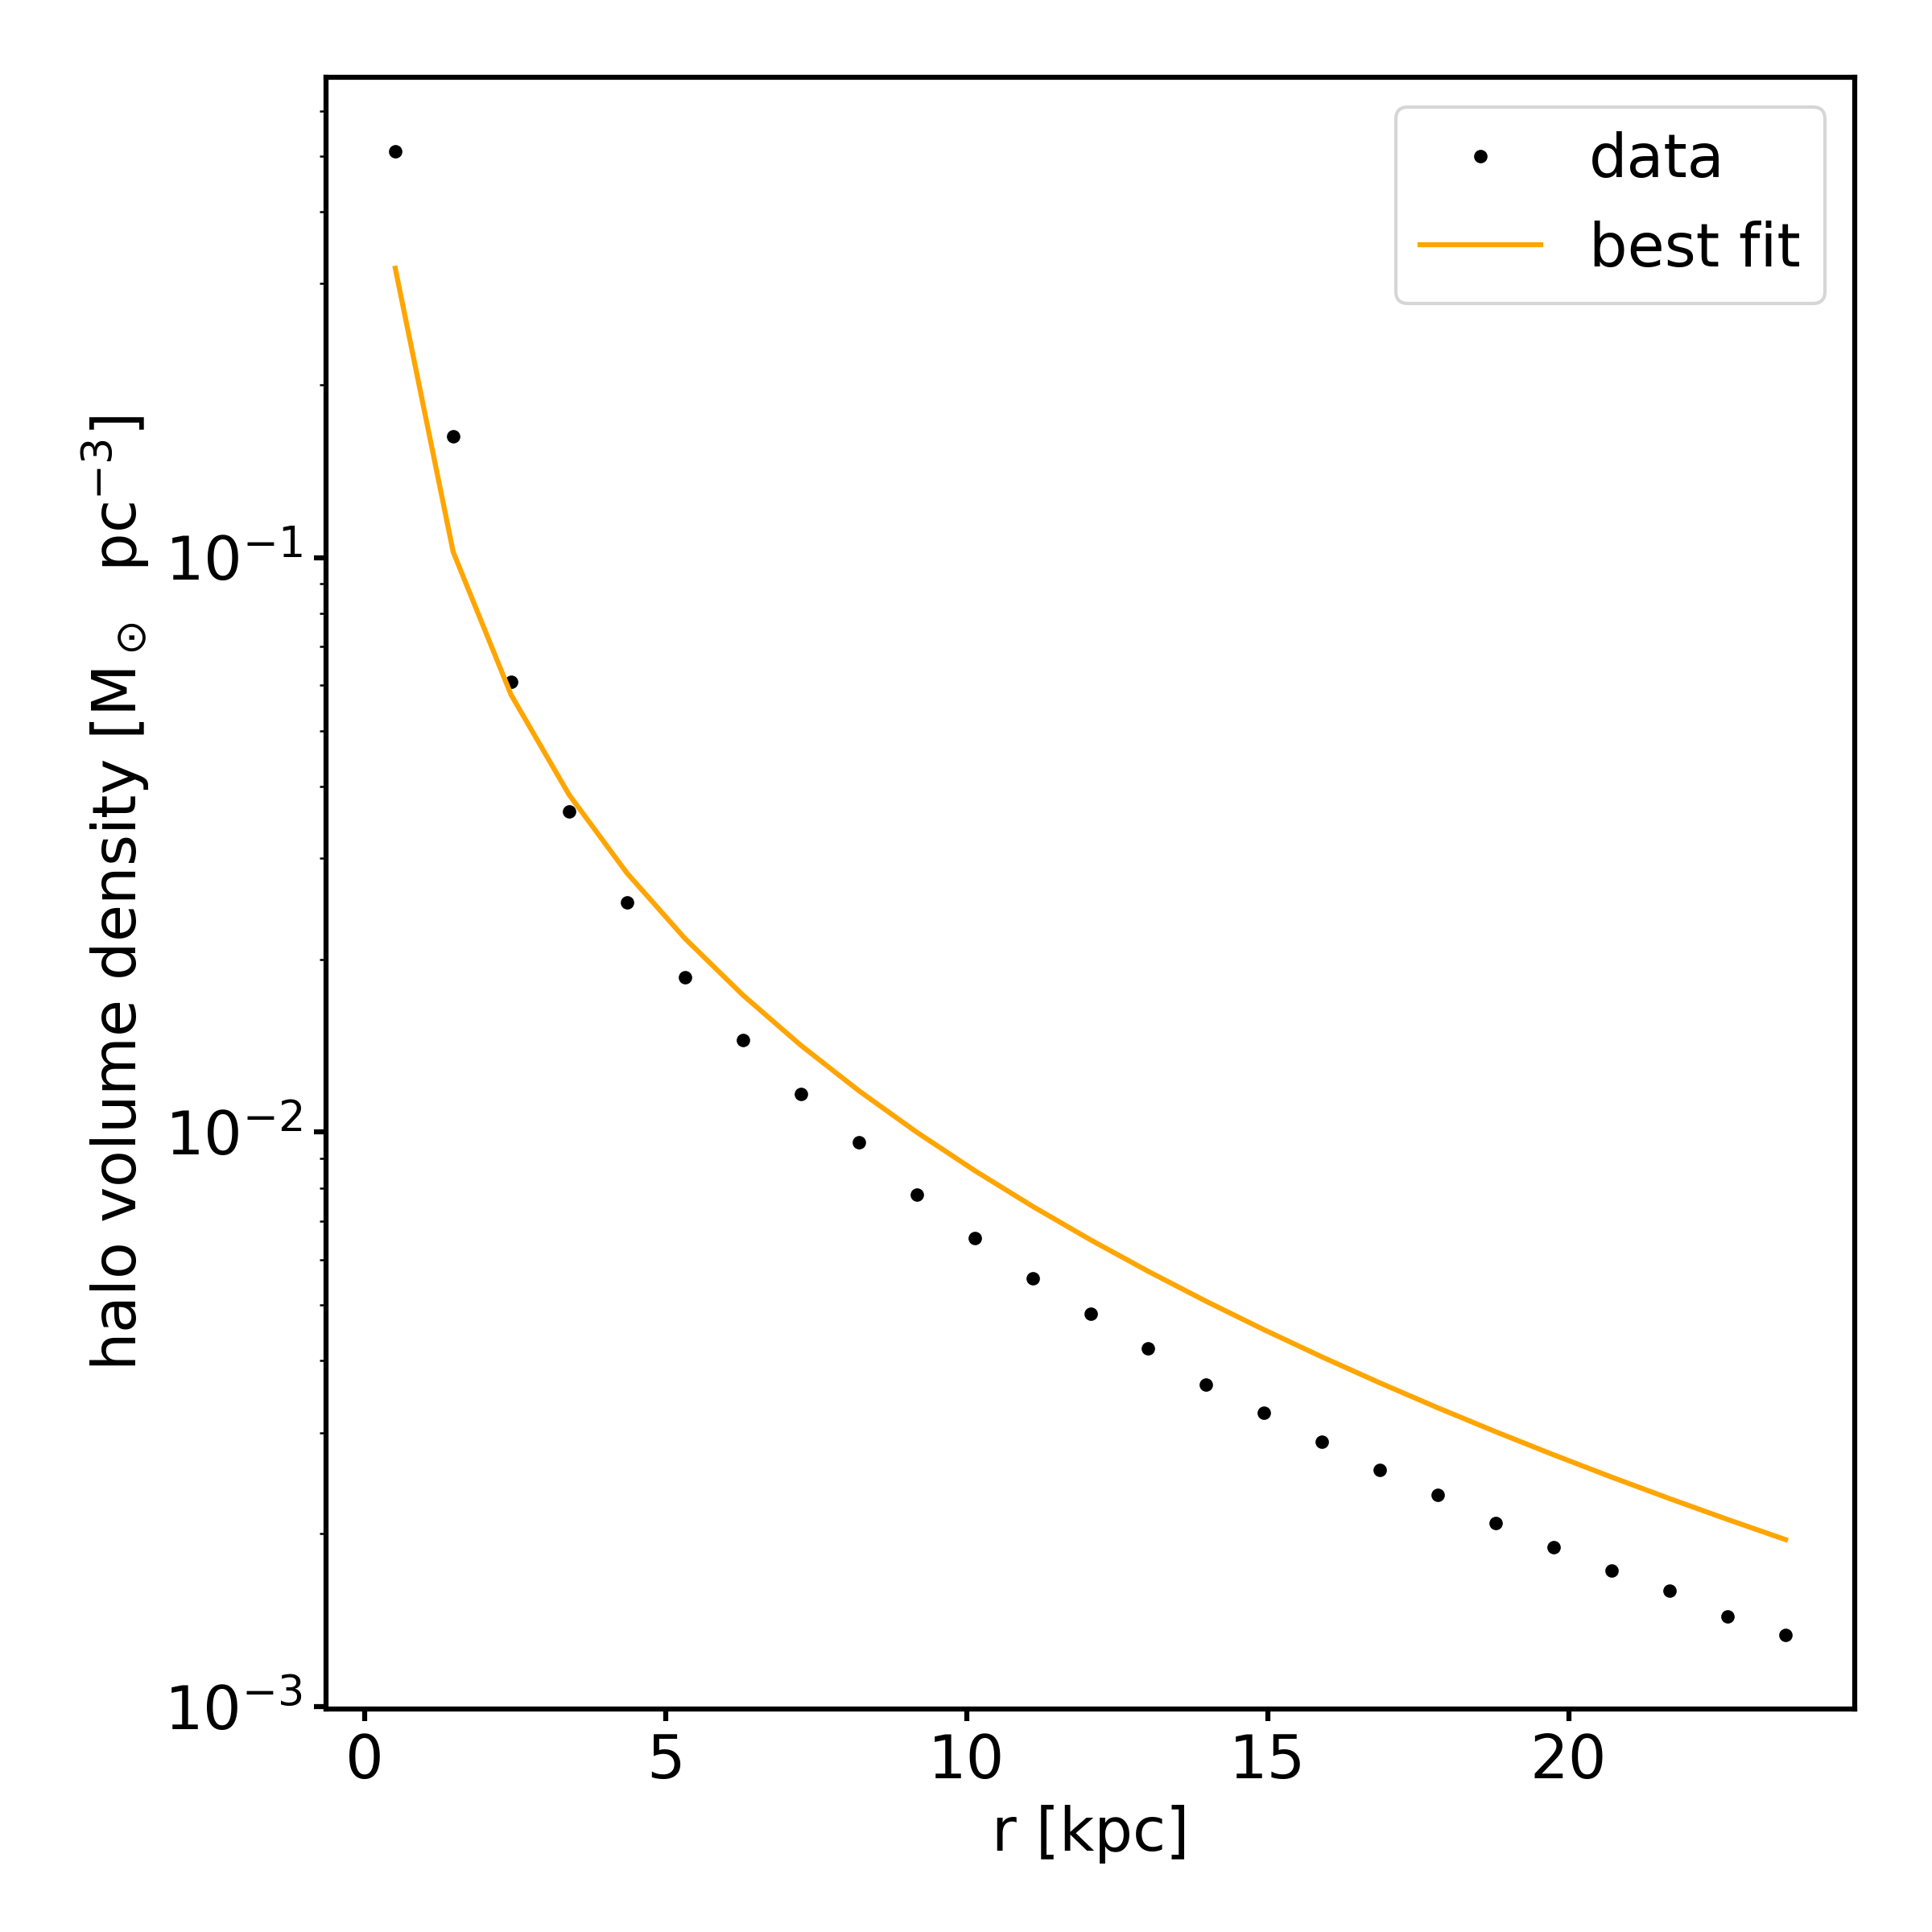
\includegraphics[width=\textwidth]{plots/Auriga/volume_dens_halo_fit_data.png}
	    \label{fig:halo_voldens_fit}
    \end{subfigure}
    \caption{Surface densities (upper row) and mass densities (lower row) of the components and their best fits at $\textit{z}=0$. Left (blue): stellar disk, middle (green): stellar spheroid, right (yellow): \ac{DM} halo.}\label{fig:single_pot_fits}
\end{figure}
\fi
\\
\begin{figure}[htbp]
\captionsetup{format=plain}
\centering
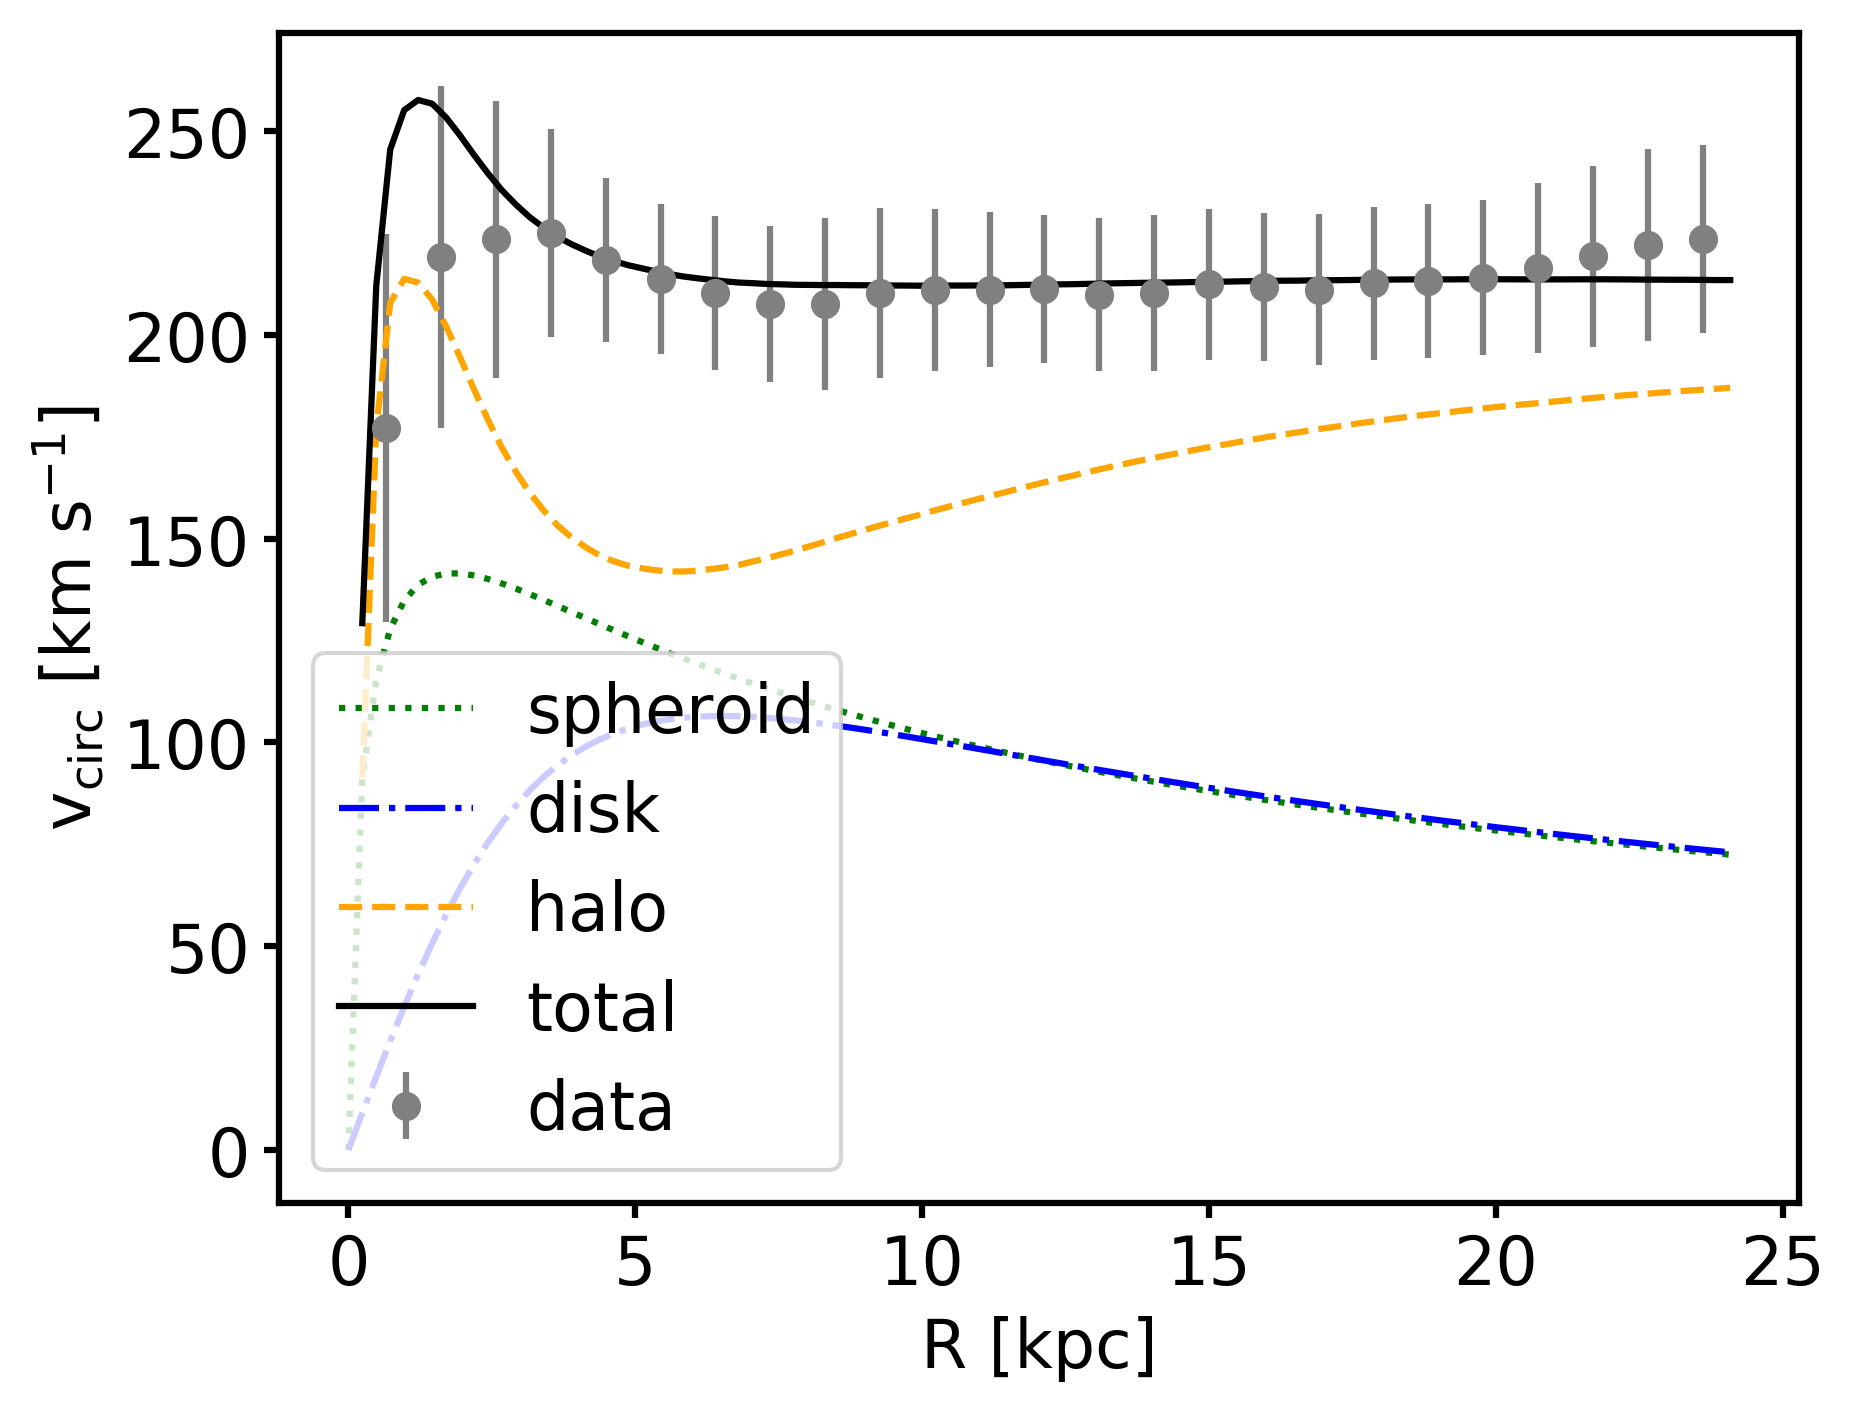
\includegraphics[width=0.8\textwidth]{plots/Auriga/best_fit_circular_velocity_via_formula_snap_127.png}
\caption{Circular velocity at \textit{z} = 0: data (grey circles), total (black solid line), disk (blue dashed dotted line), bulge (green dotted line) and halo (orange). The data is the mean tangential velocity of all stars which have $\epsilon > 0.95$. The other components and the total distribution are calculated analytically. The total curve matches the data within its errors. Disk and spheroid overlay in the outer parts which is due to the decomposition where their proportion is nearly $1:1$. The \ac{DM} halo dominates in this parts, as expected. In the center, the circular velocity is underestimated. This is probably due to an underestimation of the spheroid component in the center which we can see find in the density fit in Figure \ref{fig:spheroid_fit}. In the outer parts ($R>R_0$), the curves behave as they are expected to do.}. \label{fig:circ_vel_fit}
\end{figure}
\\To verify the goodness of the total potential, we show the circular velocity curve in Figure \ref{fig:circ_vel_fit}. While in the innermost part the \ac{DM} proportion might be too high due to an underestimation of the stellar spheroid, the \ac{DM} proportion in the outer part seems correct. The disk is underestimated due to the sharp decomposition. In overall, the total circular velocity matches the data and the fit in the outer parts, where the particles we investigate in Section \ref{sec:Dynamics} are, is reliable.  

\subsubsection{Time evolution}
To make sure we can assume a slowly varying potential and to carry out investigations of e.g. the action evolution we need to know the potential for each snapshot. Using the fitting routine, we fit  a potential to each snapshot individually, without taking the results of the neighbouring snapshots into account, e.g. as a prior. Therefore, the fitting of the time evolution is unbiased in that sense. 
\begin{figure}%[htbp]
\captionsetup{format=plain}
\centering
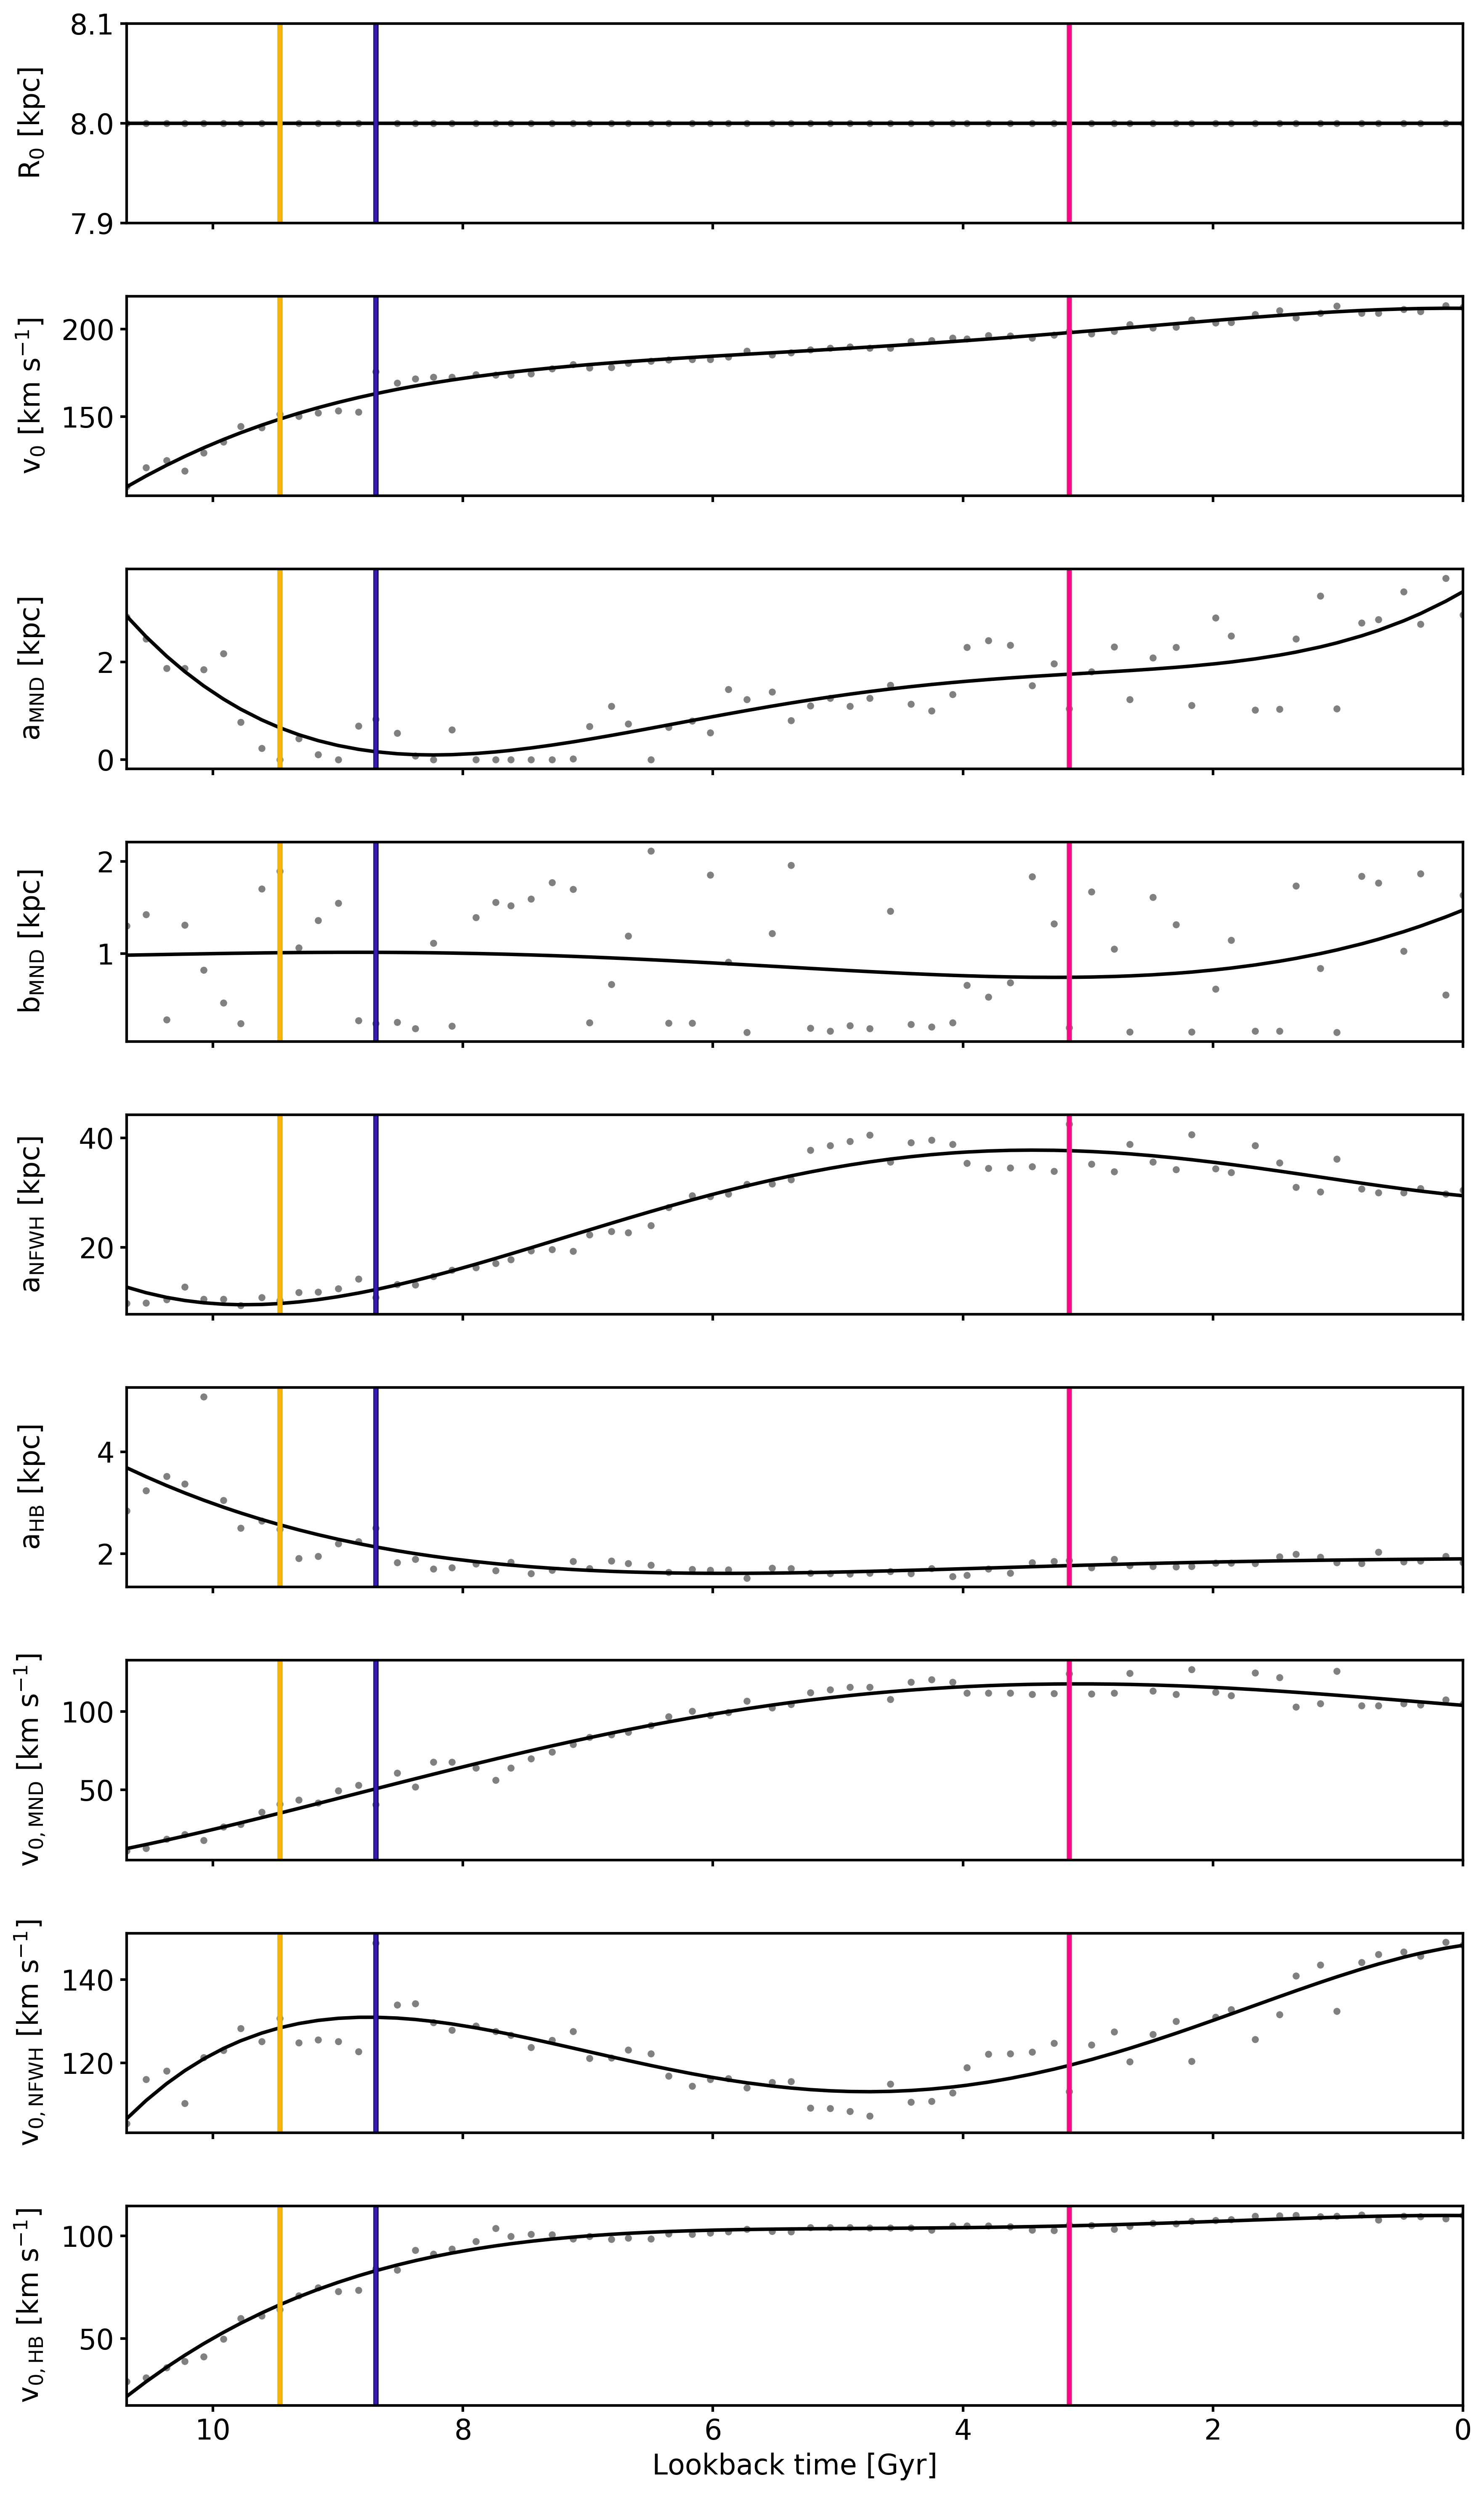
\includegraphics[width=0.7\textwidth]{plots/Auriga/fitted_potential_evolution_jan19.png}
\caption{Evolution of all fit parameters over time. $R_0$ and $v_0$ describe the overall evolution and the other parameters describe scale length - and height, if applicable - and their contribution to the circular velocity. The grey dots are the best fit values and the black lines are polynomial fits of 4th order for each parameter. The vertical lines mark the merger times of the three biggest merger events the main halo galaxy has experiences. The pink merger was the latest and biggest merger while the yellow merger contributed the least mass of these. In the first two panels, we see that the growth of the galaxy is continuous. The second merger flattened out the rise of the total circular velocity which is measured at $R_0 = \SI{8}{kpc}$. It is kept constant throughout the time evolution to see how within a constant radius the mass changes over time. The spheroid's parameters are very constant since the second merger, while the disk and the \ac{DM} halo are affected by the last merger. While the disk seems to grow in size, its contribution to the total circular velocity decreases. On the contrary, the \ac{DM} halo contracts but its contribution to the velocity rises more steeply. This shows, that these mergers have a strong impact on the evolution of the potential of this galaxy. Nevertheless, with the fits of the values we can still assume a slowly varying potential which is essential for the action evolution.}\label{fig:pot_val_evol}
\end{figure}
In Figure \ref{fig:pot_val_evol}, we show the time evolution of the potential parameters for the last \SI{10.5}{Gyr}. In the potential parameters, we see how the galaxy grows and how the growth is affected by mergers. The indicated mergers are described in more detail in the next Section and in Table \ref{tab:prog_overview}. The overall trend is very smooth and without any outliers. The spheroid remains very constant after the second biggest merger while the other components, especially the disk, have a larger scatter. The latest and biggest merger has a strong impact on the disk and the \ac{DM} halo. The fits of the values allow us to still carry out the action investigations (from Section \ref{subsec:GCs_action_space} on) under the assumption of a slowly varying potential (see also Section 3.6.1 in \citealp{Binney...Tremaine...2008}). 

\subsection{What not to do when fitting a gravitational potential to simulations}\label{subsec:wrong_pot_fit}
Even though the total circular velocity of our model matches the data the single component fits we carry out in Section \ref{subsec:best_fit_pot} have regions with large errors. We now explain some of the steps we took to develop this algorithm, what did not work and how we can deal with these errors.

\textbf{Fit the potential in one step}
In the first try, we worked with the three component analytic potential as well but we assumed that we can just fit the combined potential to the 'pot' value of a different amount of random particles (up to 1 million) of the simulation data. It resulted in a big overestimation of the halo and we had not control in giving each component its proportion.

\textbf{Decomposition}
To then fit a potential to each component we carried out a decomposition (Section \ref{subsubsec:decomp}). This decomposition only takes dynamically cold disk particles into account and does not set boundaries on the disk height. We therefore probably underestimated the disk while still having spheroid particles above and below the disk. Doing the decomposition kinematically is a good start but the recipe could expanded by some more complex disk characteristics. To get around the decomposition one could try to fit all stellar particles to a combination of disk and spheroid potential.

\textbf{Binning and weighting of the data}
Once we made a selection of disk and spheroid particles, we had to bin our densities to fit models to them. Depending on bin distances (e.g. linear or logarithmic), sizes and weights the focus of the fit is given to particular regions of the data. This has to be taken into account when preparing the data to be fitted.

\textbf{Fitting routines}
There are many methods of fitting models to data and these different methods offer a wide range of different implementations. We tried several for the different components. The first we used was scipy.optimize.minimize looking for the minimum of the relative error between data and model. This fitting routine find local minima. Therefore it sometimes ran into very unphysical parameters and found them to be the best fit. This routine was therefore to simple. We tried fitting the parameters with 'emcee' \textcolor{red}{reference} but this took very long and did not always converge so it was also not the best choice for us. Another scipy.optimize routine is 'differential\_evolution' which finds the global minima. So here again we minimized the relative error. This worked on the 1D models in the spherical potentials but did not in the 2D \ac{MN} potential as the algorithm just tried to set the model to 0 which would give in a small relative error but it resulted in extremely flat and elongated disks ($a_\mathrm{MND} = $ upper boundary and $b_\mathrm{MND} = 0$. The last fitting routine we then used on the \ac{MN} disk was scipy.optimize.curve\_fit which fits absolute differences between data and model but only requires the binned density and the model as input without the need to define how it minimizes the problem. This then worked for the disk the best. 

\textbf{Find proper fitting characteristics}
We fitted the stellar components to the stellar densities and the \ac{DM} profile to the potential value. We could also consider fitting all three components to their circular velocities which can also be calculated by the models. This would give us a constrain from the dynamical side and could make the fit better.

\\\\ Taking into account all these steps which we have to consider fitting a potential and getting still such a good circular velocity curve (Figure \ref{fig:circ_vel_fit} in the end, we are confident that this potential we got is good enough to carry out further investigations in this model but we also want to emphasize that this is a big component which can be improved.


%\textbf{Put in table with parameter comparison }

\section[Adaptive dynamics]{Adaptive dynamics: Can actions of accreted globular clusters constrain the gravitational potential?}\label{sec:Dynamics}

\subsection{Integrals of motion}
This Section is based on \S3.1, \S3.2 and \S3.5 of \citet{Binney...Tremaine...2008}. Objects (e.g., stars and \acp{GC}) in gravitational potential move on orbits which are described by their positions and velocities in 6 dimensional phase space, (\textbf{x}, \textbf{v}). Functions $I$, which are constant along an orbit, are called \acf{IoM} \citep{Binney...Tremaine...2008}:
\begin{equation}
    I[\mathbf{x}(t_1), \mathbf{v}(t_1)] = I[\mathbf{x}(t_2), \mathbf{v}(t_2)]
\end{equation}
for any $t_1$ and $t_2$. This means, that the time derivative of these \ac{IoM} is 0:
\begin{equation}\label{eq:der_IoM}
    0 = \dot{I}
\end{equation}
In an axisymmetric 3D potential as we assumed and fitted in Section \ref{sec:Auriga} orbits can have up to three \ac{IoM}. 
\subsubsection{Energy and angular momentum}
Energy E and some components of the angular momentum \textbf{L}, depending on the symmetry of the potential, are regarded as classical \ac{IoM}. In a spherical potential, all three components of $\textbf{L} = \textbf{x} \times \textbf{v}$ are \ac{IoM} while in the axisymmetric potential $\Phi$ only the axis, around which the potential is symmetric, is the component of the angular momentum which is the integral of motion (usually $L_z$). The energy is given by the Hamiltonian H,
\begin{equation}\label{eq:energy_hamiltonian}
    H(\mathbf{x, v}) = \frac{1}{2}v^2 + \Phi(\mathbf{x}) = E
\end{equation}
with the total velocity $v$. In an axisymmetric potential, the \ac{IoM} ($E,L_z$) are supplemented by a third integral of motion, $I_3 =$ constant, which, in general, does not have an analytic expression and therefore is a non-classical integral. 
\subsubsection{Actions}
\textbf{General introduction to actions} A particular set of \ac{IoM} are actions which, together with angles, create a canonical coordinate system. These actions are three momenta, $\mathbf{J} = (J_1, J_2, J_3)$, which describe the whole orbit while the angles, $\bm{\theta} = (\theta_1, \theta_2, \theta_3) $ define the position of the object on the orbit. Orbits for which actions can be calculated are called regular orbits. The three actions are given by the integral
\begin{equation}
    J_i = \frac{1}{2\pi}\oint_{\gamma_i}\mathbf{p}\cdot\mathrm{d}\mathbf{q} \qquad i = 1,2,3
\end{equation}
over the path $\gamma_i$ with vector $\mathbf{q}(t)$ and corresponding momentum $\mathbf{p}(t)$ given a Hamiltonian system which satisfies 
\begin{equation}
    \dot{\mathbf{q}} = \frac{\partial H}{\partial \mathbf{p}} \quad;\quad \dot{\mathbf{p}} = - \frac{\partial H}{\partial \mathbf{q}}. 
\end{equation}
The range of the angles is by construction $\theta_i = [0,2\pi]$ so that it moves periodically around the center of the galaxy. Since $0 = \dot{J} = -\partial H / \partial\theta_i$ (Equation \ref{eq:der_IoM}), the Hamiltonian is independent of $\bm{\theta}$. Therefore, angles follow the time evolution
\begin{equation}
    \dot{\theta}_i = \frac{\partial H}{\partial J_i} \equiv \Omega_i(\mathbf{J}), \quad \mathrm{a\ constant} \quad \Rightarrow\quad \theta_i(t) = \theta_i(0) +  \Omega_i t
\end{equation}
with the fundamental frequencies $\Omega_i$. The components of $\bm{\theta}$ evolve linearly in time. 
\\\\\textbf{Definition in cylindrical coordinates} In the axisymmetric potential we have the spatial coordinates $(R, \phi, z)$ and velocities $(v_R, v_\phi, v_z)$ which we can use for the planes ($x_i, v_i$) in which we examine the actions $\mathbf{J} = (J_R, J_\phi = L_z, J_z)$. The actions quantify the oscillation of the orbit in the given coordinate direction. $J_R$ describes how the object moves towards and away from the galactic center, the radial oscillation, and $J_z$ the oscillation above and below the equatorial plane while $J_\phi = L_z$ is the angular momentum along the symmetry axis. Circular orbits do not oscillate in $R$ and $z$ so the actions in these directions are ($J_R, J_z$) = 0.

\textbf{Numerical calculation of actions} Only in a simple spherical symmetric potential, the Isochrone potential $\Phi(r) = -GM/b + \sqrt{b^2+r^2}$ with scale length $b$, actions can be calculated analytically without at single integration. To numerically calculate the actions of objects in our axisymmetric potential from Section \ref{sec:Auriga}, we need to use approximations. Axisymmetric potentials could for example be treated like St\"ackel potentials \citep{deZeeuw...Staeckel..1985} which have the form
\begin{equation}\label{eq:Stackel_pot}
    \Phi(u,v) = \frac{U(u)-V(v)}{\sinh^2u + \sin^2v}
\end{equation}
with $(u,v)$ defined by 
\begin{equation}
    R = \Delta \sinh{u} \sin{v}\quad ; \quad z = \Delta \cosh{u}\cos{v}
\end{equation}
even if they are not perfect St\"ackel potentials. This method is called St\"ackel Fudge \citep{Binney...StaeckelFudge...2012}. This algorithm is implemented in galpy and we use is for the action calculations
\textcolor{red}{Bisschen anschaulicher erklaren. Focallaänge erwaähnen und sagen wie ich sie mitgenommen hab.}


\iffalse
\subsection{Merger tree}
We say th
figure: Merger tree of Auriga 24. 
\fi
\subsection{Globular cluster sample selection}\label{subsec:GC_selection}
Due to the resolution of the simulation, $M = 5 \cdot 10 ^ 4\ \mathrm{M}_{\odot}$, we set one stellar particle as one \ac{GC}. All stellar particles which were accreted by the main halo are followed through the evolution and kept as accreted \acp{GC} as long as they do not cross the disk in a sense that they either are directly in the disk - defined empirically per snapshot as within the disk radius $R_\mathrm{d} = 0.05  R_{200}$ and the height $z_\mathrm{d} = 0.03\ R_\mathrm{d}$ - to match the \ac{MW} disk's scale height in the $z = 0$ snapshot - since we assume that in that case the \ac{GC} would be disrupted. 

\begin{table}[htbp]
\captionsetup{format=plain}
    \caption{Progenitor parameters. The selected progenitors ar}

    \centering
    \begin{tabular}{@{}lllll@{}}
        \toprule
         \makecell[l]{name}& \makecell[l]{merger time [Gyr]}& \makecell[l]{num of \\accreted particles} & \makecell[l]{total mass of \\accreted particles} & Dwarf to galaxy mass [$10^11 \mathrm{M}_\odot$]\\
         \midrule
         prog2& 3.15 & && &\\
         prog3& 8.70 & &&&\\
         prog4& 9.46 & &&&
         \bottomrule
    \end{tabular}
    \label{tab:prog_overview}
\end{table}
 We select the three biggest merger events and present their properties in Table \ref{tab:prog_overview}. In einer externen Galaxie will man die DGs mithilfe der Age-Metallicity Relation auseinander klamüsern. Je größer der Dwarf, desto mehr GCs, desto eher kann der Merger Event und die dazugehörigen GCs identifiziert werden.

\begin{figure}[htbp]
\captionsetup{format=plain}

    \centering
    \begin{subfigure}[c]{0.48\textwidth}
    \centering
    	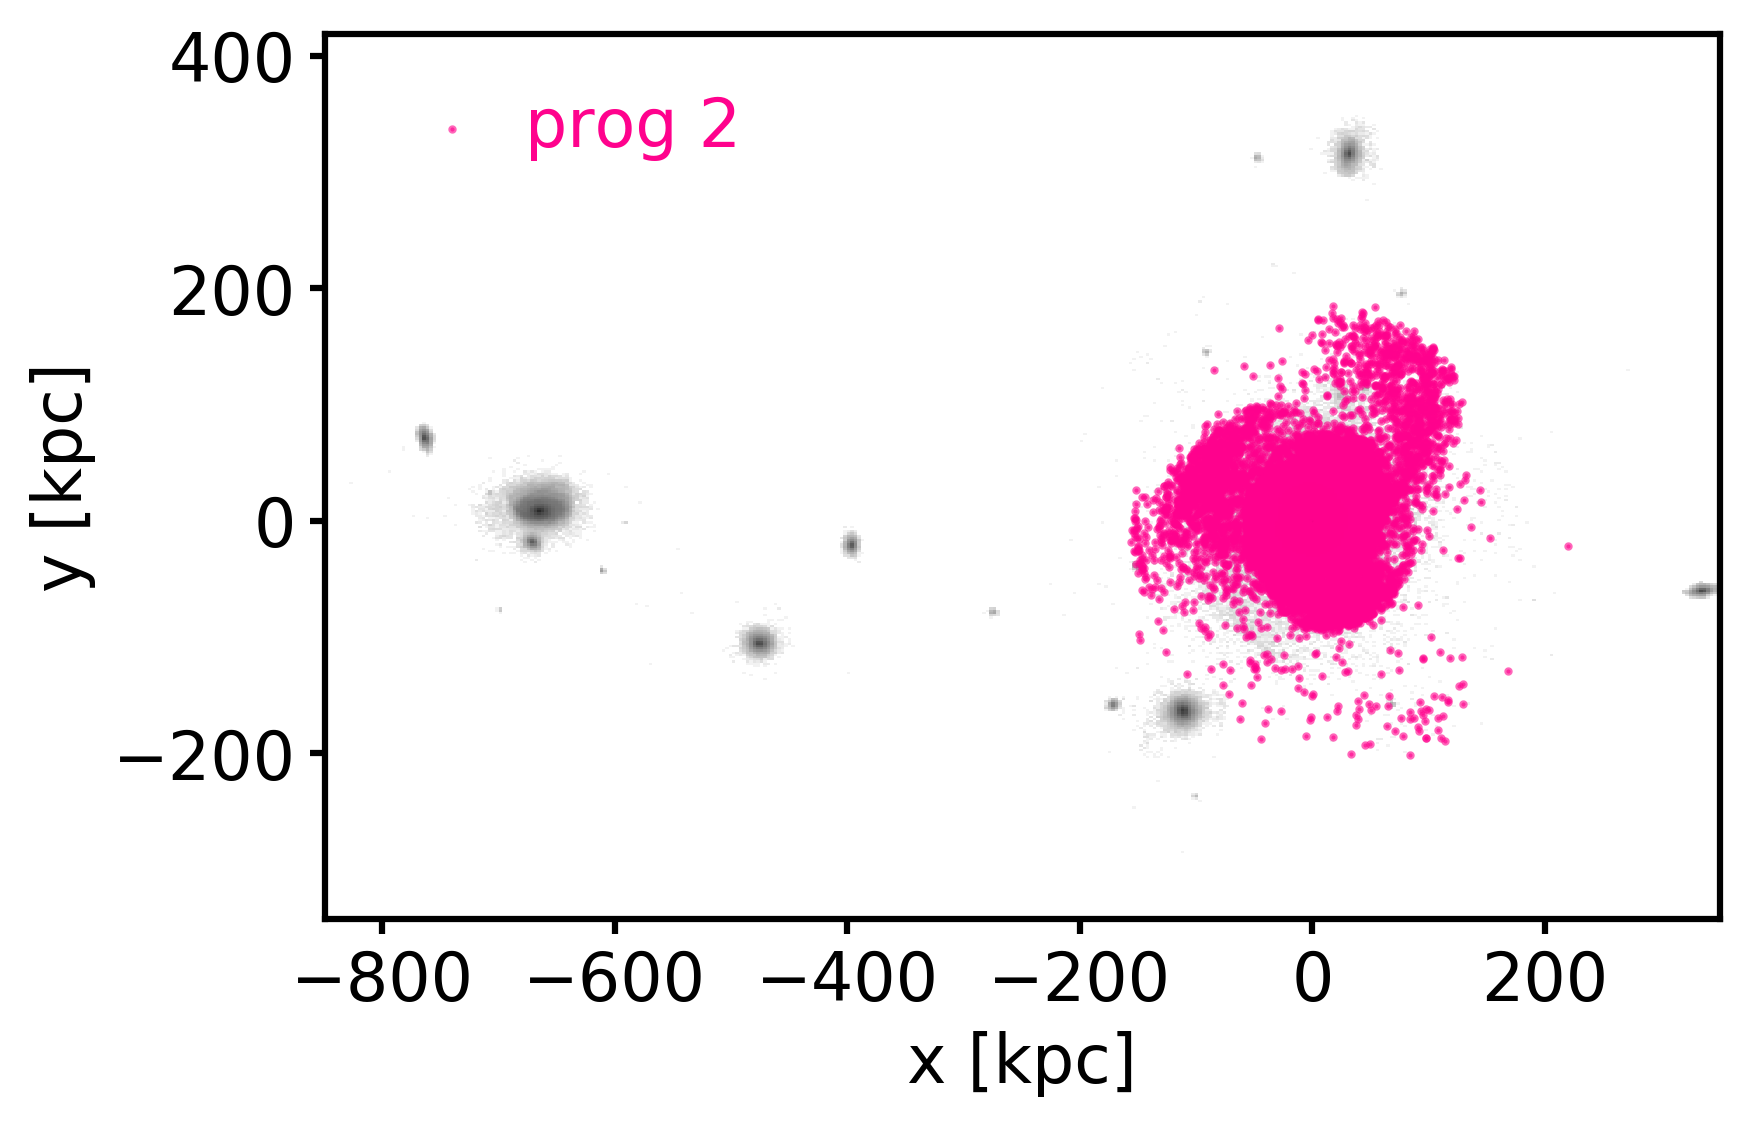
\includegraphics[width=\textwidth]{plots/Dynamics/dist/xy_dist_wodisk_GCs_prog_2_snap_127.png}
    	\label{fig:prog2_xy}
    \end{subfigure}
    ~ %add desired spacing between images, e. g. ~, \quad, \qquad, \hfill etc. 
    %(or a blank line to force the subfigure onto a new line)
    \begin{subfigure}[c]{0.48\textwidth}
        \centering
    	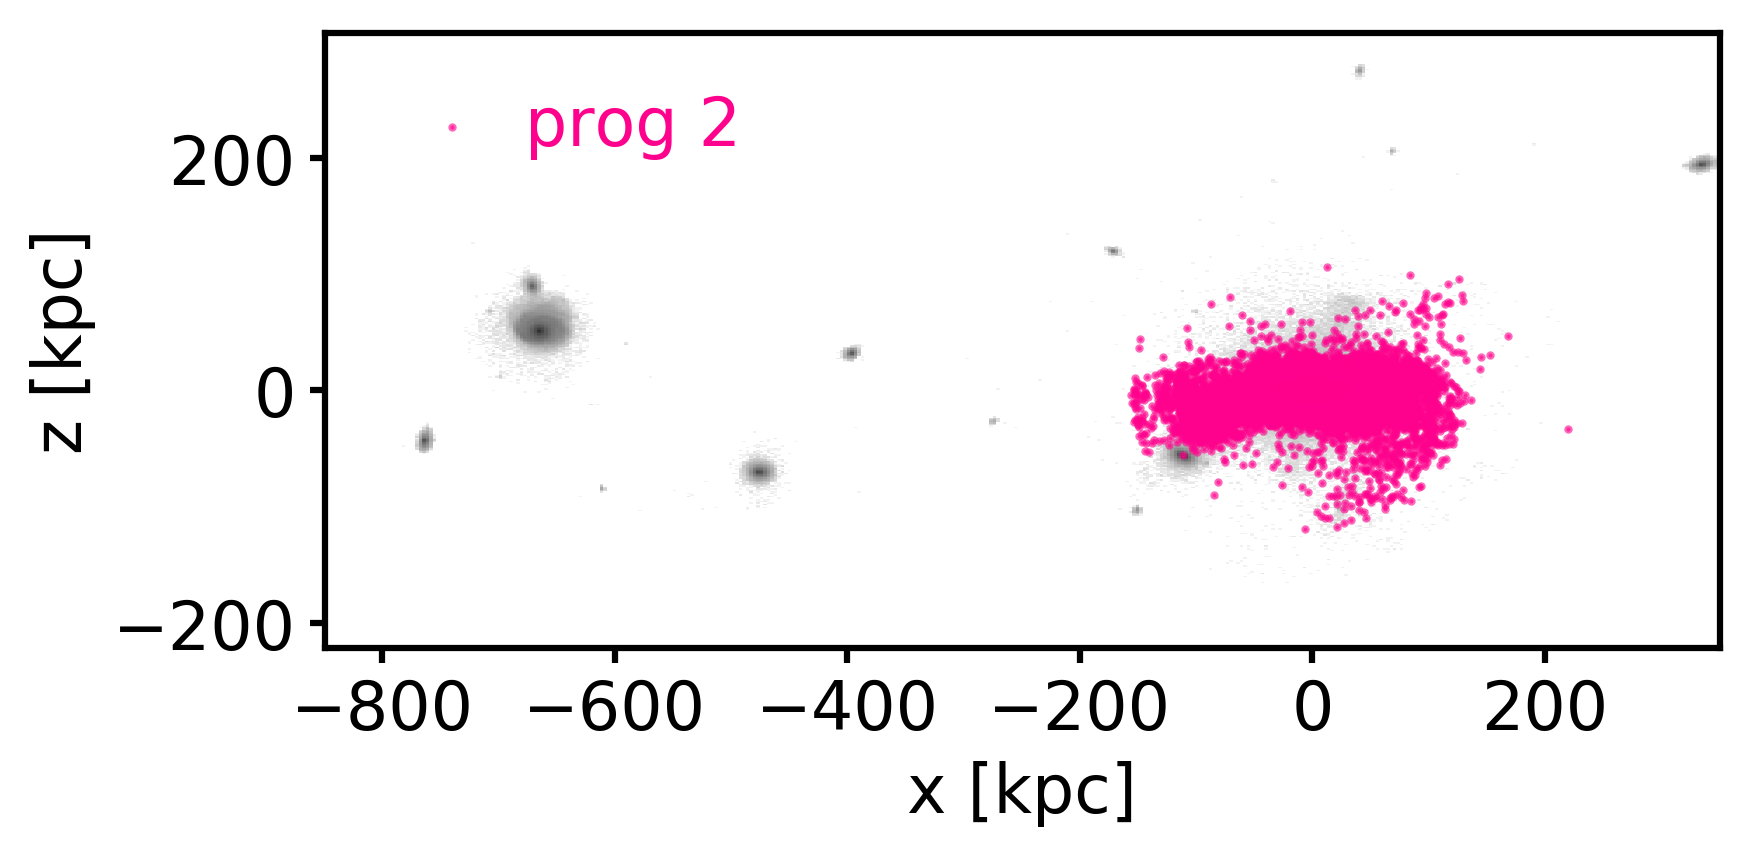
\includegraphics[width=\textwidth]{plots/Dynamics/dist/xz_dist_wodisk_GCs_prog_2_snap_127.png}
	    \label{fig:prog2_xz}
    \end{subfigure}
    
    \begin{subfigure}[c]{0.48\textwidth}
    \centering
    	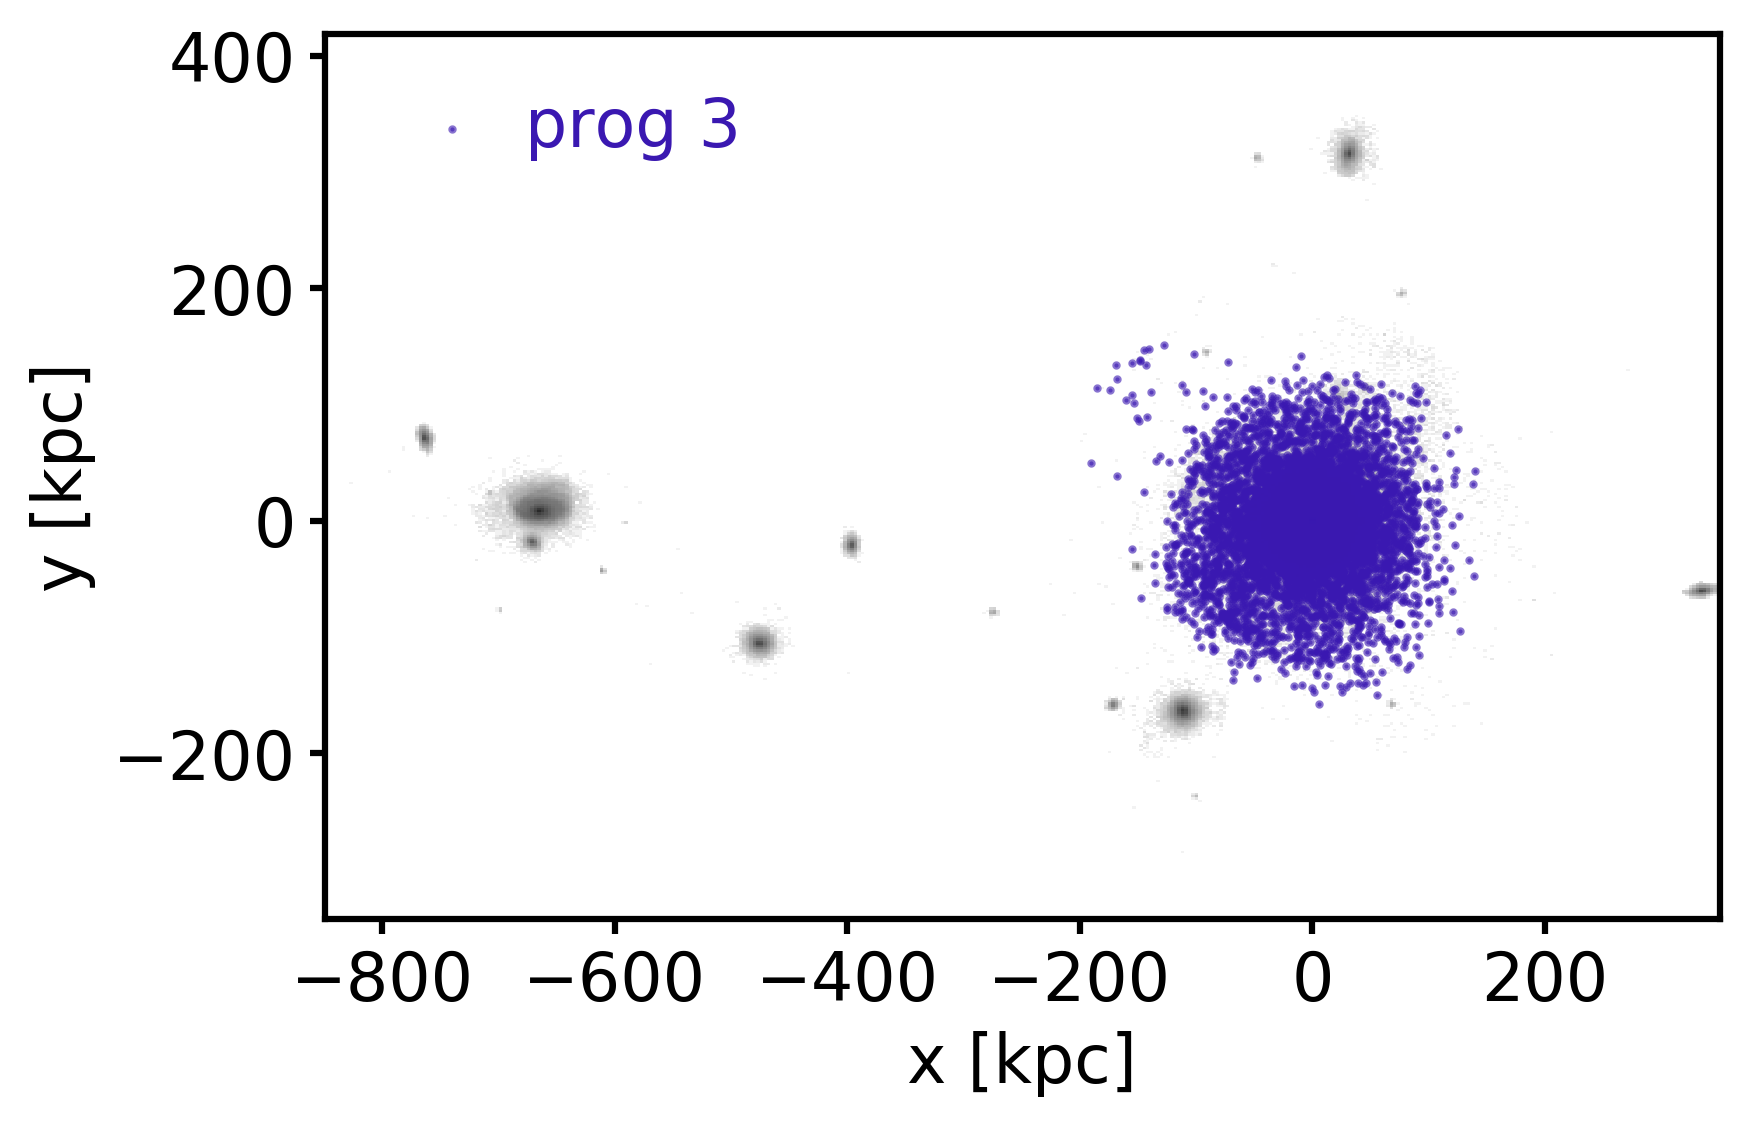
\includegraphics[width=\textwidth]{plots/Dynamics/dist/xy_dist_wodisk_GCs_prog_3_snap_127.png}
    	\label{fig:prog3_xy}
    \end{subfigure}
    ~ %add desired spacing between images, e. g. ~, \quad, \qquad, \hfill etc. 
    %(or a blank line to force the subfigure onto a new line)
    \begin{subfigure}[c]{0.48\textwidth}
        \centering
    	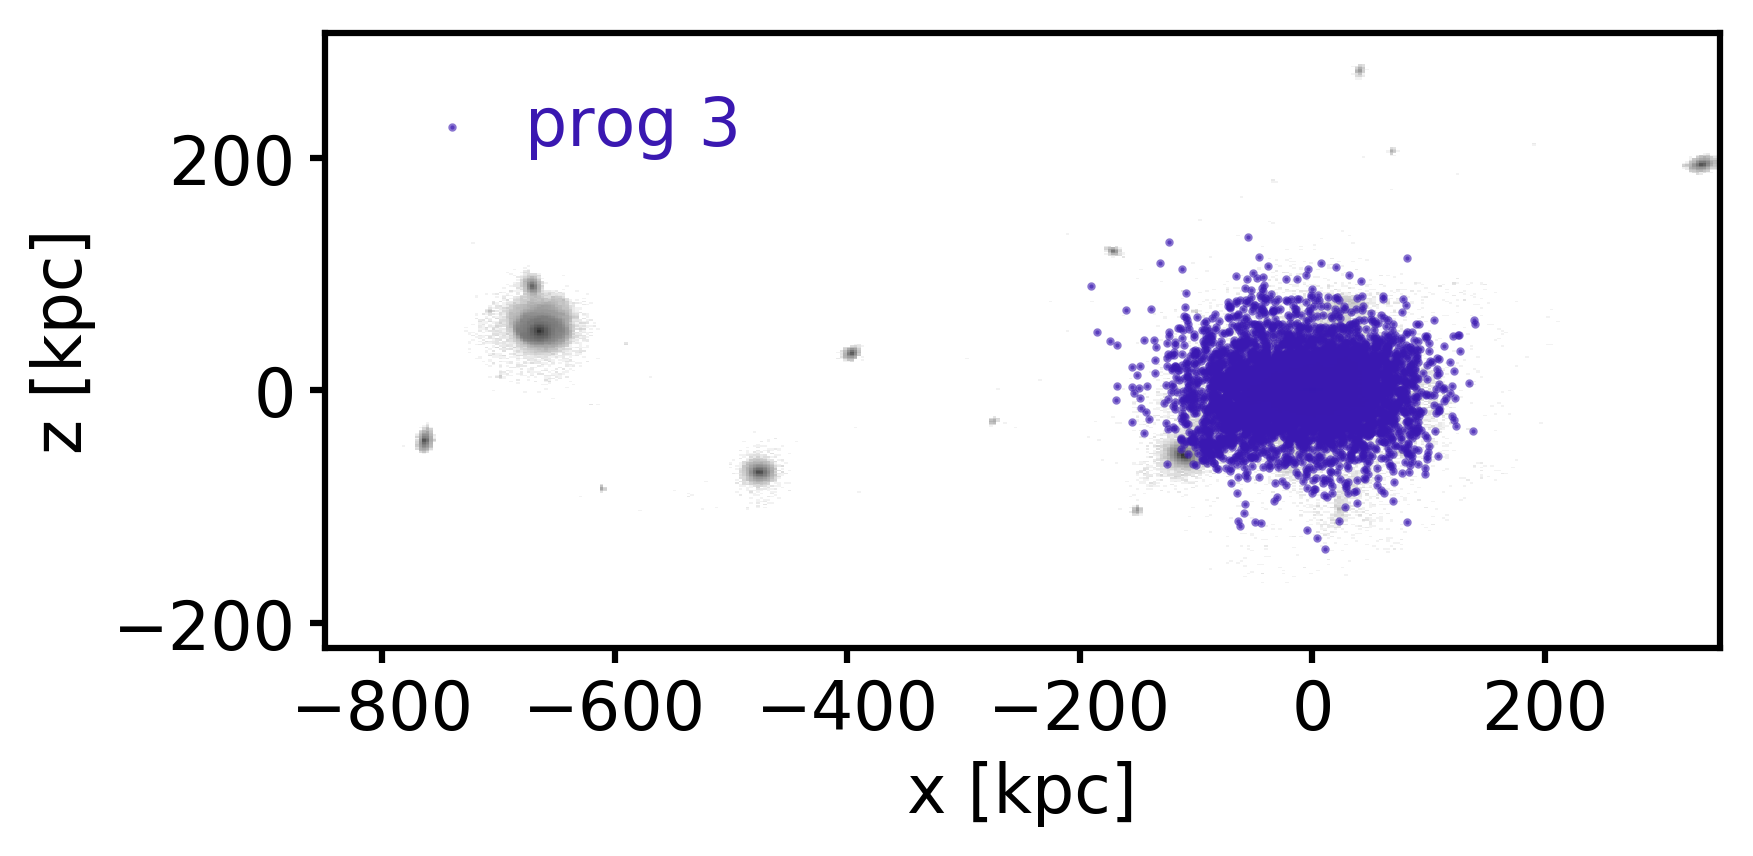
\includegraphics[width=\textwidth]{plots/Dynamics/dist/xz_dist_wodisk_GCs_prog_3_snap_127.png}
	    \label{fig:prog3_xz}
    \end{subfigure}
    
    \begin{subfigure}[c]{0.48\textwidth}
    \centering
    	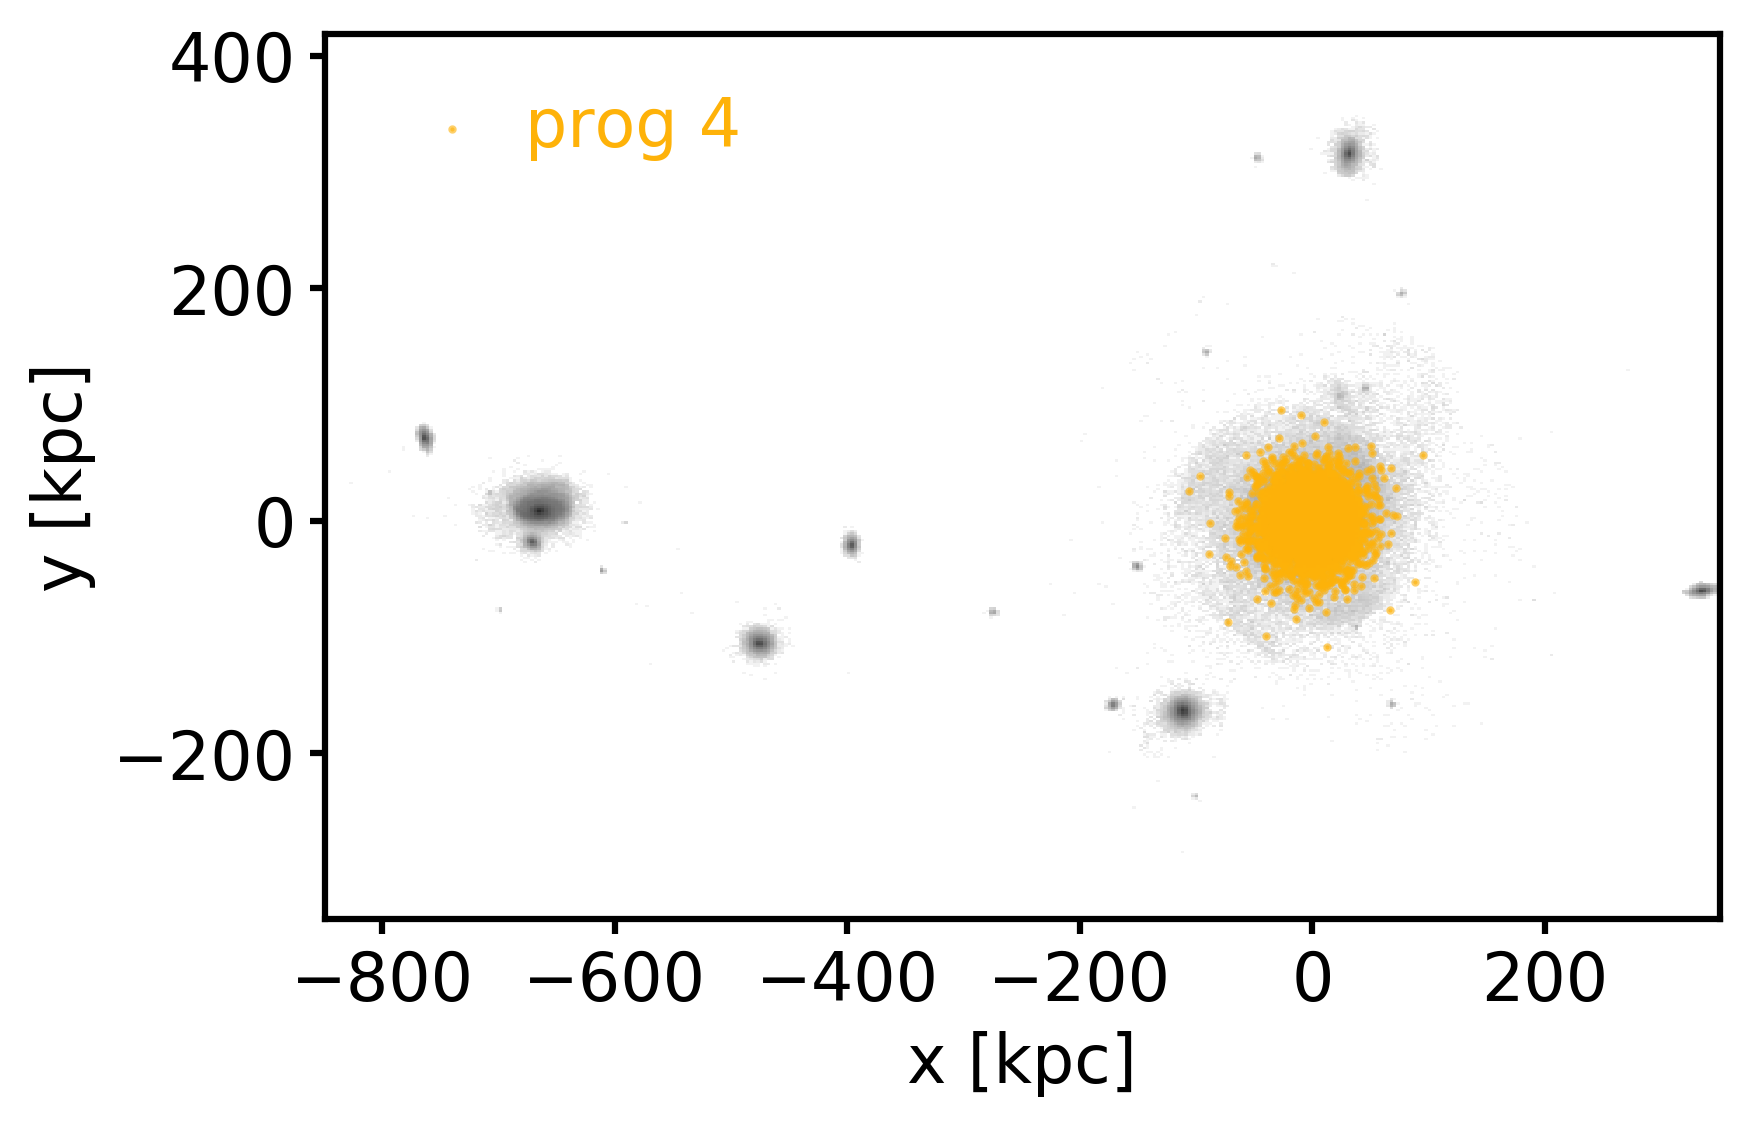
\includegraphics[width=\textwidth]{plots/Dynamics/dist/xy_dist_wodisk_GCs_prog_4_snap_127.png}
    	\label{fig:prog4_xy}
    \end{subfigure}
    ~ %add desired spacing between images, e. g. ~, \quad, \qquad, \hfill etc. 
    %(or a blank line to force the subfigure onto a new line)
    \begin{subfigure}[c]{0.48\textwidth}
        \centering
    	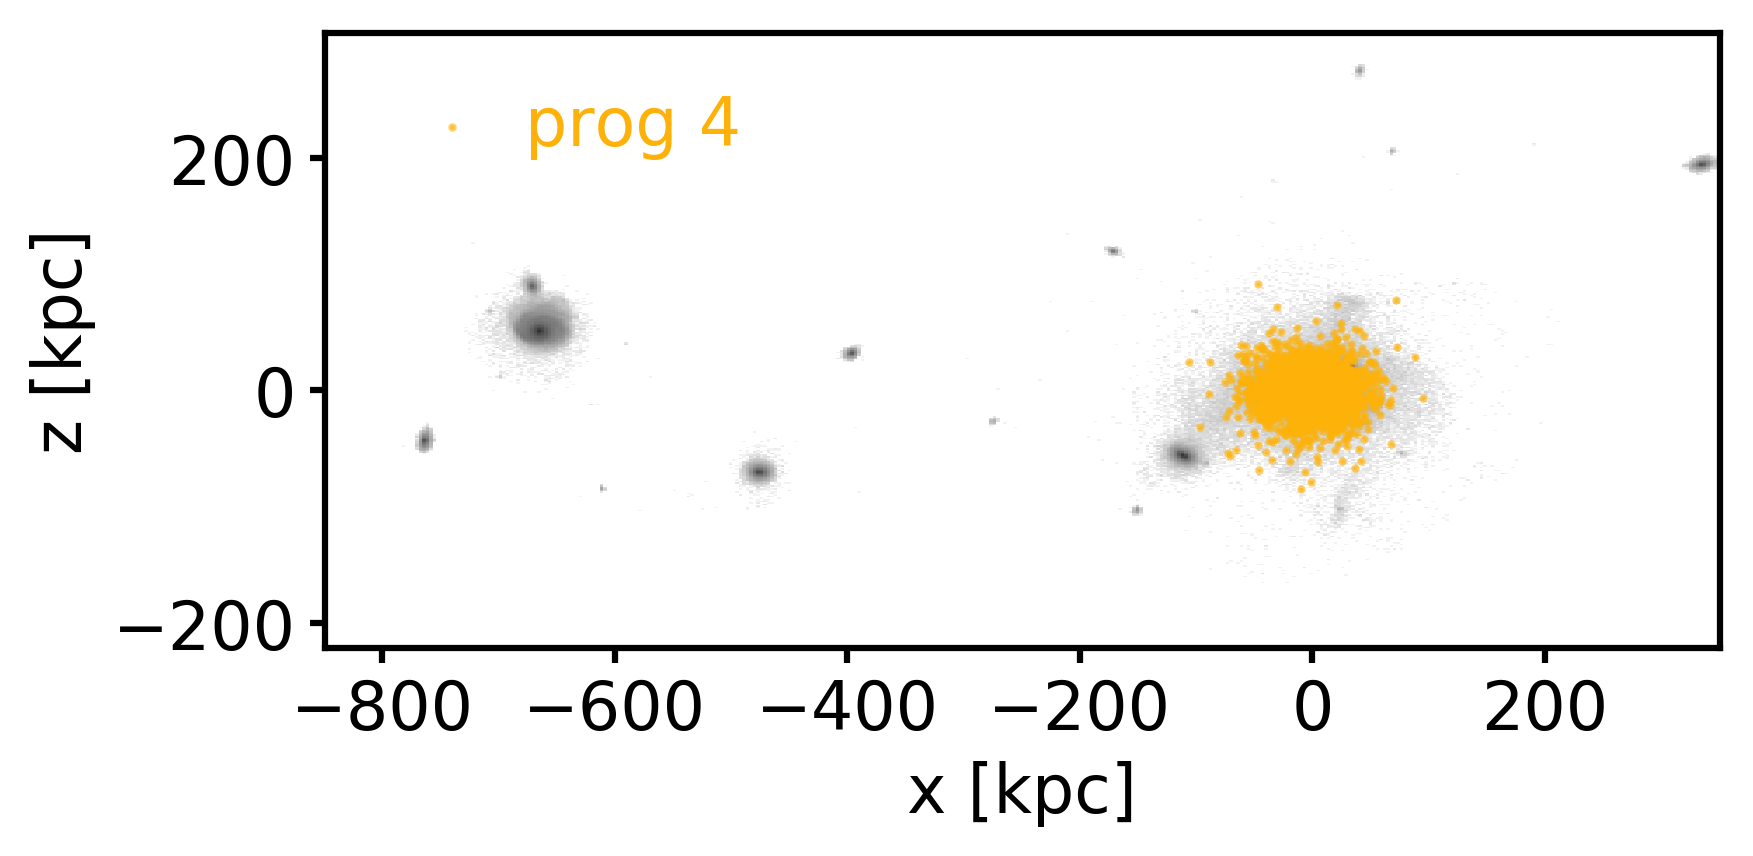
\includegraphics[width=\textwidth]{plots/Dynamics/dist/xz_dist_wodisk_GCs_prog_4_snap_127.png}
	    \label{fig:prog4_xz}
    \end{subfigure}
    \caption{Remnants of the three biggest \ac{DG} mergers which were not destroyed by the disk. The left panels show the x-y number distribution, the right panels the x-z distribution. In grey, the main galaxy and its satellites are plotted (as in Figure \ref{fig:Stars_AU24}). \textit{Upper panels}: The remnants of the most recent merger are plotted in pink. \textit{Middle panel}: The blue points are remnants of the second biggest merger. \textit{Lower panel}: The yellow points are remnants of the third biggest merger which is the most long ago of these three. These remnants will be considered the \ac{GC} populations of each merger event.}\label{fig:progenitors_distribution}
\end{figure}
The positions of the remnants of these three merger events are shown in Figure \ref{fig:progenitors_distribution}. Prog3 and prog4 are totally dispersed in the galaxy while prog2 still shows some merging features such as broad streams, especially visible face-on. Prog2 has nearly a factor of 100 more remaining \acp{GC} than the other two progenitors. This is due to the short time it is in the main galaxy and therefore \textcolor{red}{rewrite:could these \acp{GC} are neither as much dissolved as the others nor as much disrupted by the disk}. Since these three mergers are so different at redshift 0, it is interesting to test their behaviour in action space, which is useful to reveal stars on common orbits. 

\subsection{Globular clusters in action space}\label{subsec:GCs_action_space}
Now, we look at the \ac{GC} distribution in action space. Our assumption is that in the "true" potential, \acp{GC} are very clumped since they should retain dynamical memory from their former \ac{DG}'s orbit and therefore their \ac{DF} should be a delta function. In section \ref{subsubsec:GCs_actions_right_pot}, we will look at the distribution in the fitted potential at redshift 0. In section \ref{subsubsec:GCs_actions_varying_pot}, we evaluate actions in varying potentials to test our assumption of \acp{GC} being most clumped in action space in the "true" potential. 

\subsubsection{Best fit potential}\label{subsubsec:GCs_actions_right_pot}

\begin{figure}[htbp]
\captionsetup{format=plain}
    \centering
    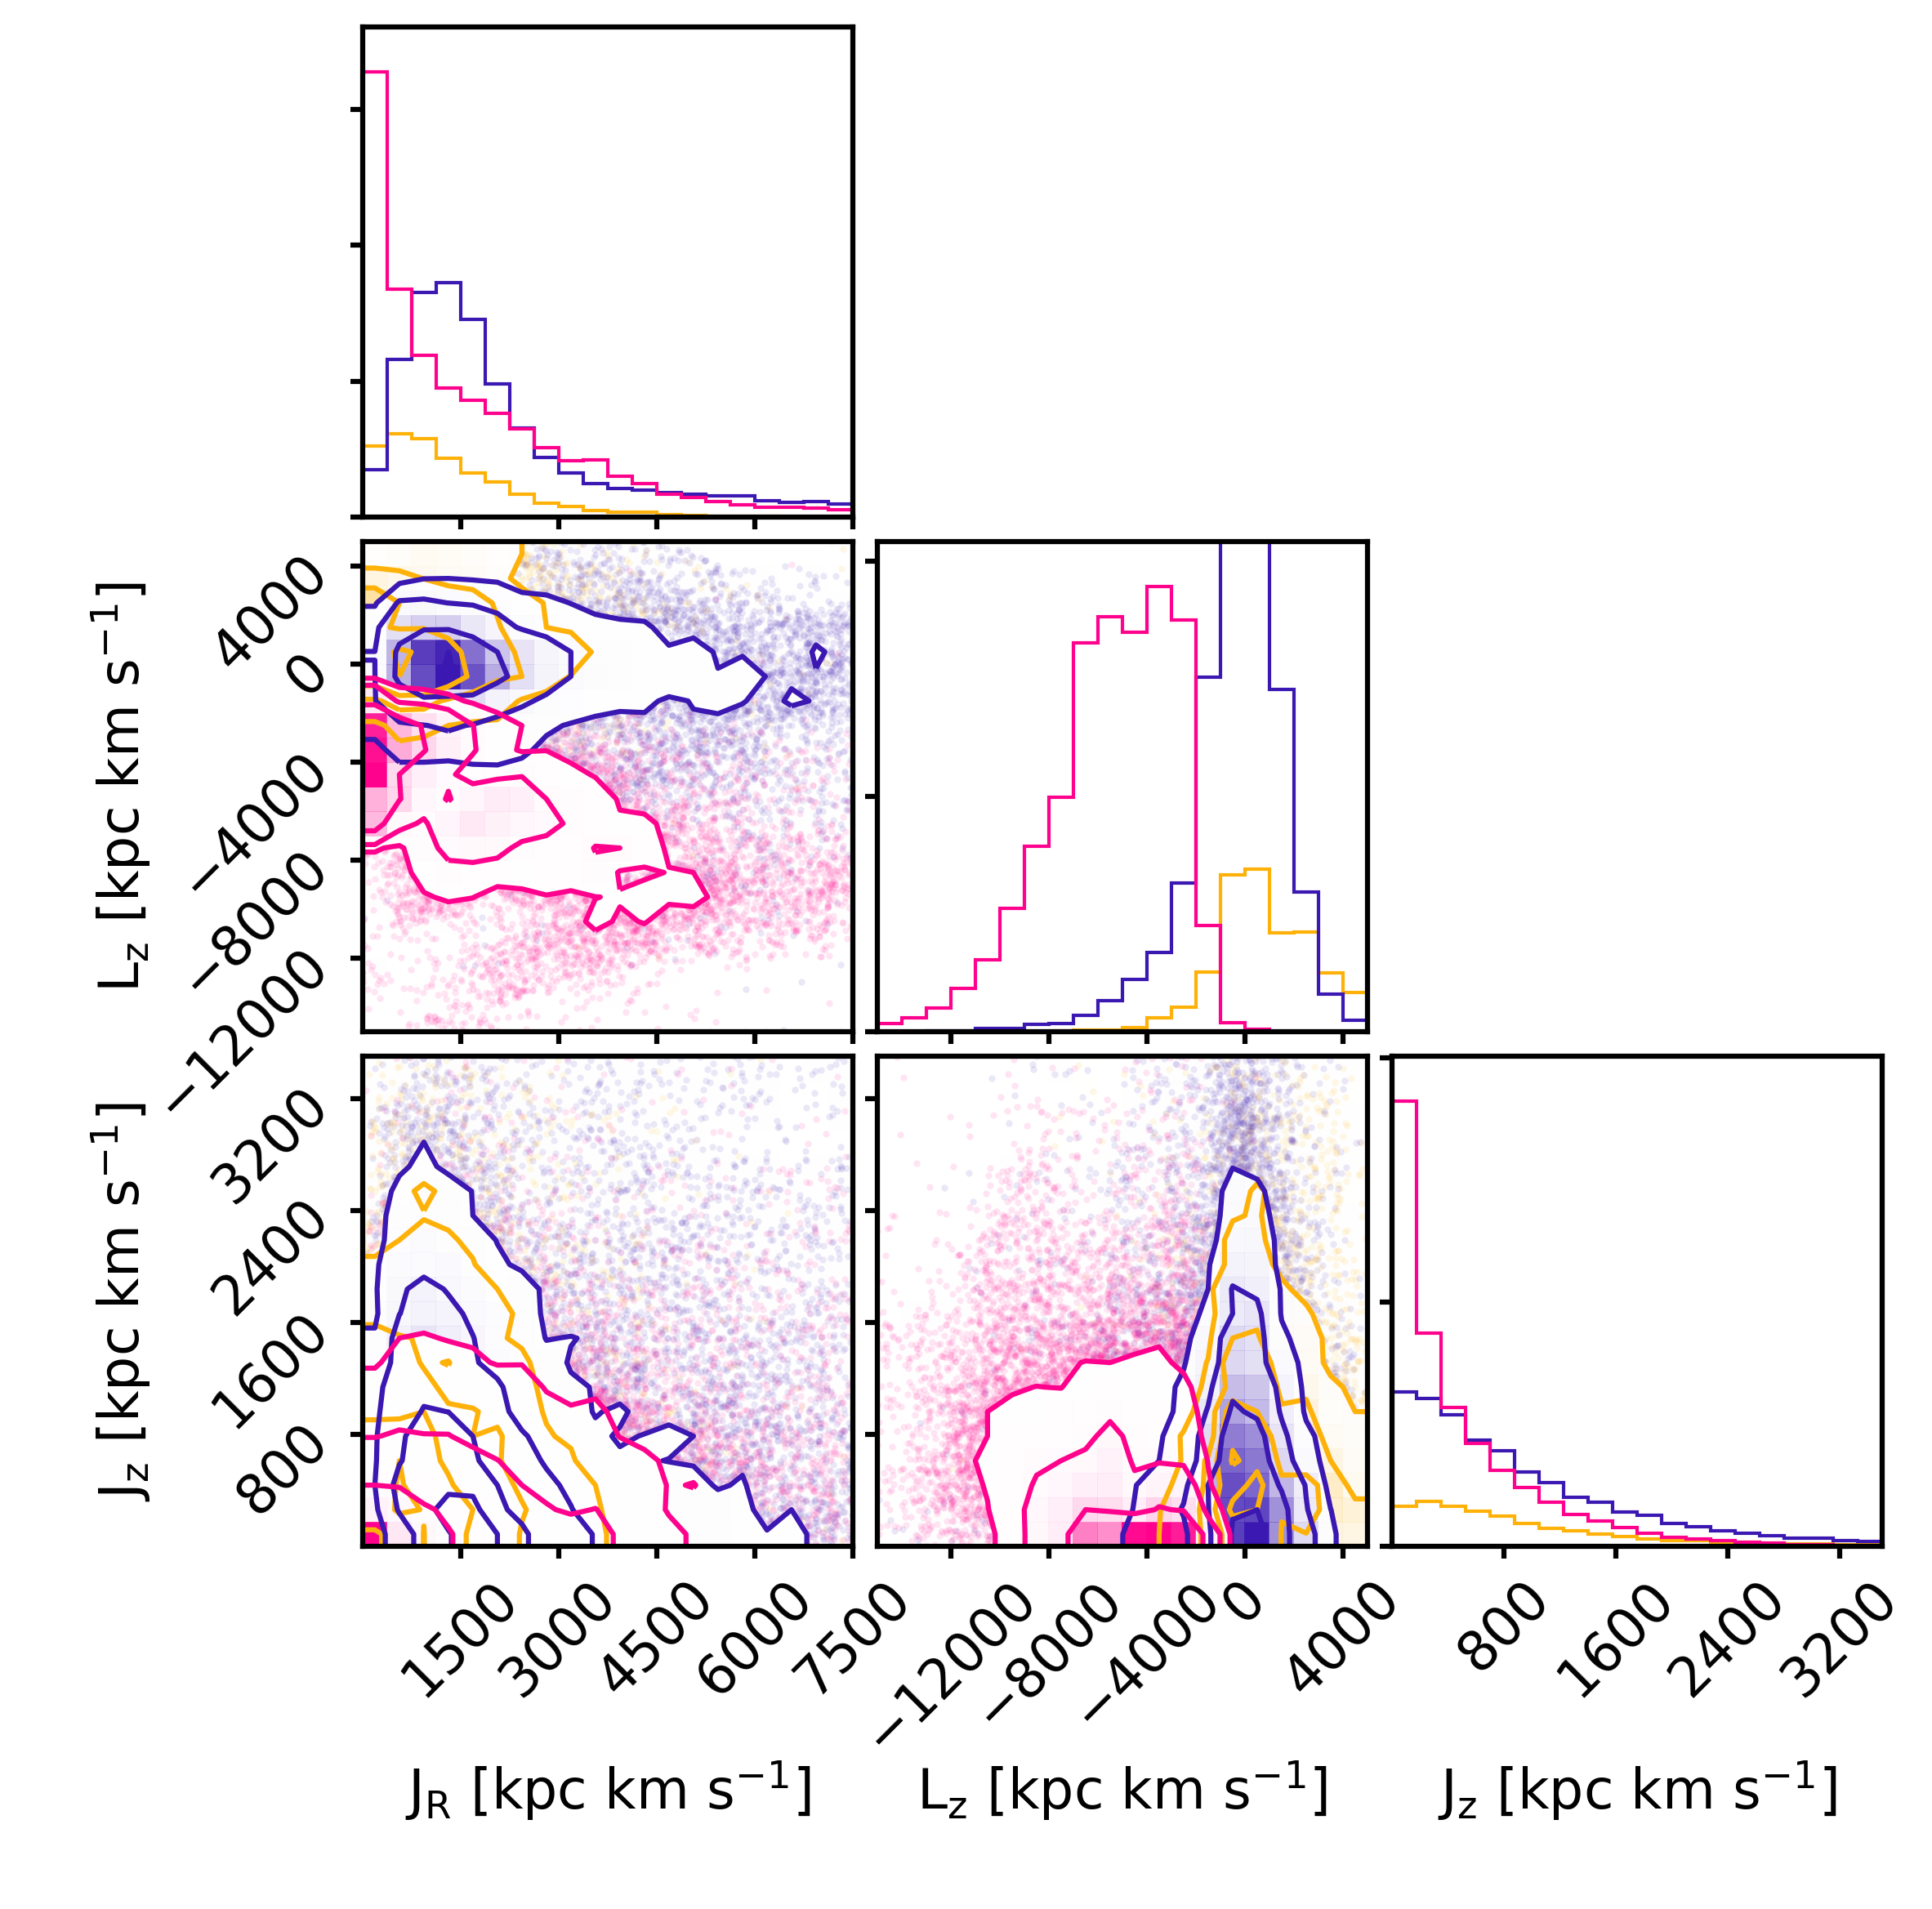
\includegraphics[width=1.0\textwidth]{plots/Dynamics/prog234_GCwodisk_actions_snap_127.png}
    \caption{Selected \acp{GC} from three different \acp{DG} in action space. The diagonal elements show histograms of each action and the other panels show 2D histograms of each action pair. In pink/blue/yellow, we see the action distribution of the remnants of prog2/prog3/prog4. Since we have many more particles from prog2, the histograms in the diagonal elements are dominated by their distribution. In the correlation panels, we can clearly distinguish prog 2 and prog 4 while prog 3 is very dispersed and does not have an identifiable center in any action. Even though the merger of prog4 happened the longest ago, it is still very clumped in all combinations, with the most clumpiness in $J_R - L_z$. The distribution of prog2 is narrow in $L_z$ but very broad in $J_R - J_z$. prog2 is corotating with the disk but with a higher angular momentum than the disk has (\(\overline{L_z} = SI{-2235}{kpc.km.s^{-1}}\)). prog4 is clearly counter rotating.}
    \label{fig:act_all_merg_best_pot}
\end{figure}
We calculate the actions of the remnants of each progenitor in the best fit potential from the coordinates ($R, \phi, z, v_r, v_\phi, v_z$) at \textit{z=0} and plot them in Figure \ref{fig:act_all_merg_best_pot}. \textcolor{red}{check plot description since it changed...}The remnants of the different merger events are best distinguishable in L$_\mathrm{Z}$. Prog2 is corotating with the disk but with higher angular momentum. Prog4 is counter rotating. Prog3 is more dispersed in L$_\mathrm{Z}$ but its mean is corotating with the disk as well. In the vertical action, the three remnant groups are not distinguishable and have means at \SI{1000-2000}{kpc.km.s^{-1}}. In J$_\mathrm{R}$, the groups are again distinguishable. 
\\The idea of this method is that in the right potential, these groups minimize their spread in action space. Prog4 is the most compact group, while especially prog3 is very dispersed. None of the distributions looks like a $\delta$-function. To quantify the compactness, we measure the standard deviation of each action. In the next Section, we compare the standard deviations of the radial and vertical actions of each group in different potentials to see, if we minimize them in the 'true' potential.

\subsubsection{Varying potentials}\label{subsubsec:GCs_actions_varying_pot}
The \acp{GC} are at distances where the potential is dominated by the \ac{DM} halo (see Figure \ref{fig:circ_vel_fit}). Variations in that component should have the biggest impact on their action space distributions. Therefore, we vary the \ac{DM} halo by keeping all best fit potential parameters constant and only vary the scale length $a_\mathrm{NFW}$. For the three groups in these potentials, we calculate the actions in the $z=0$ snapshot.
\begin{figure}[!ht]
\captionsetup{format=plain}
   \subfloat{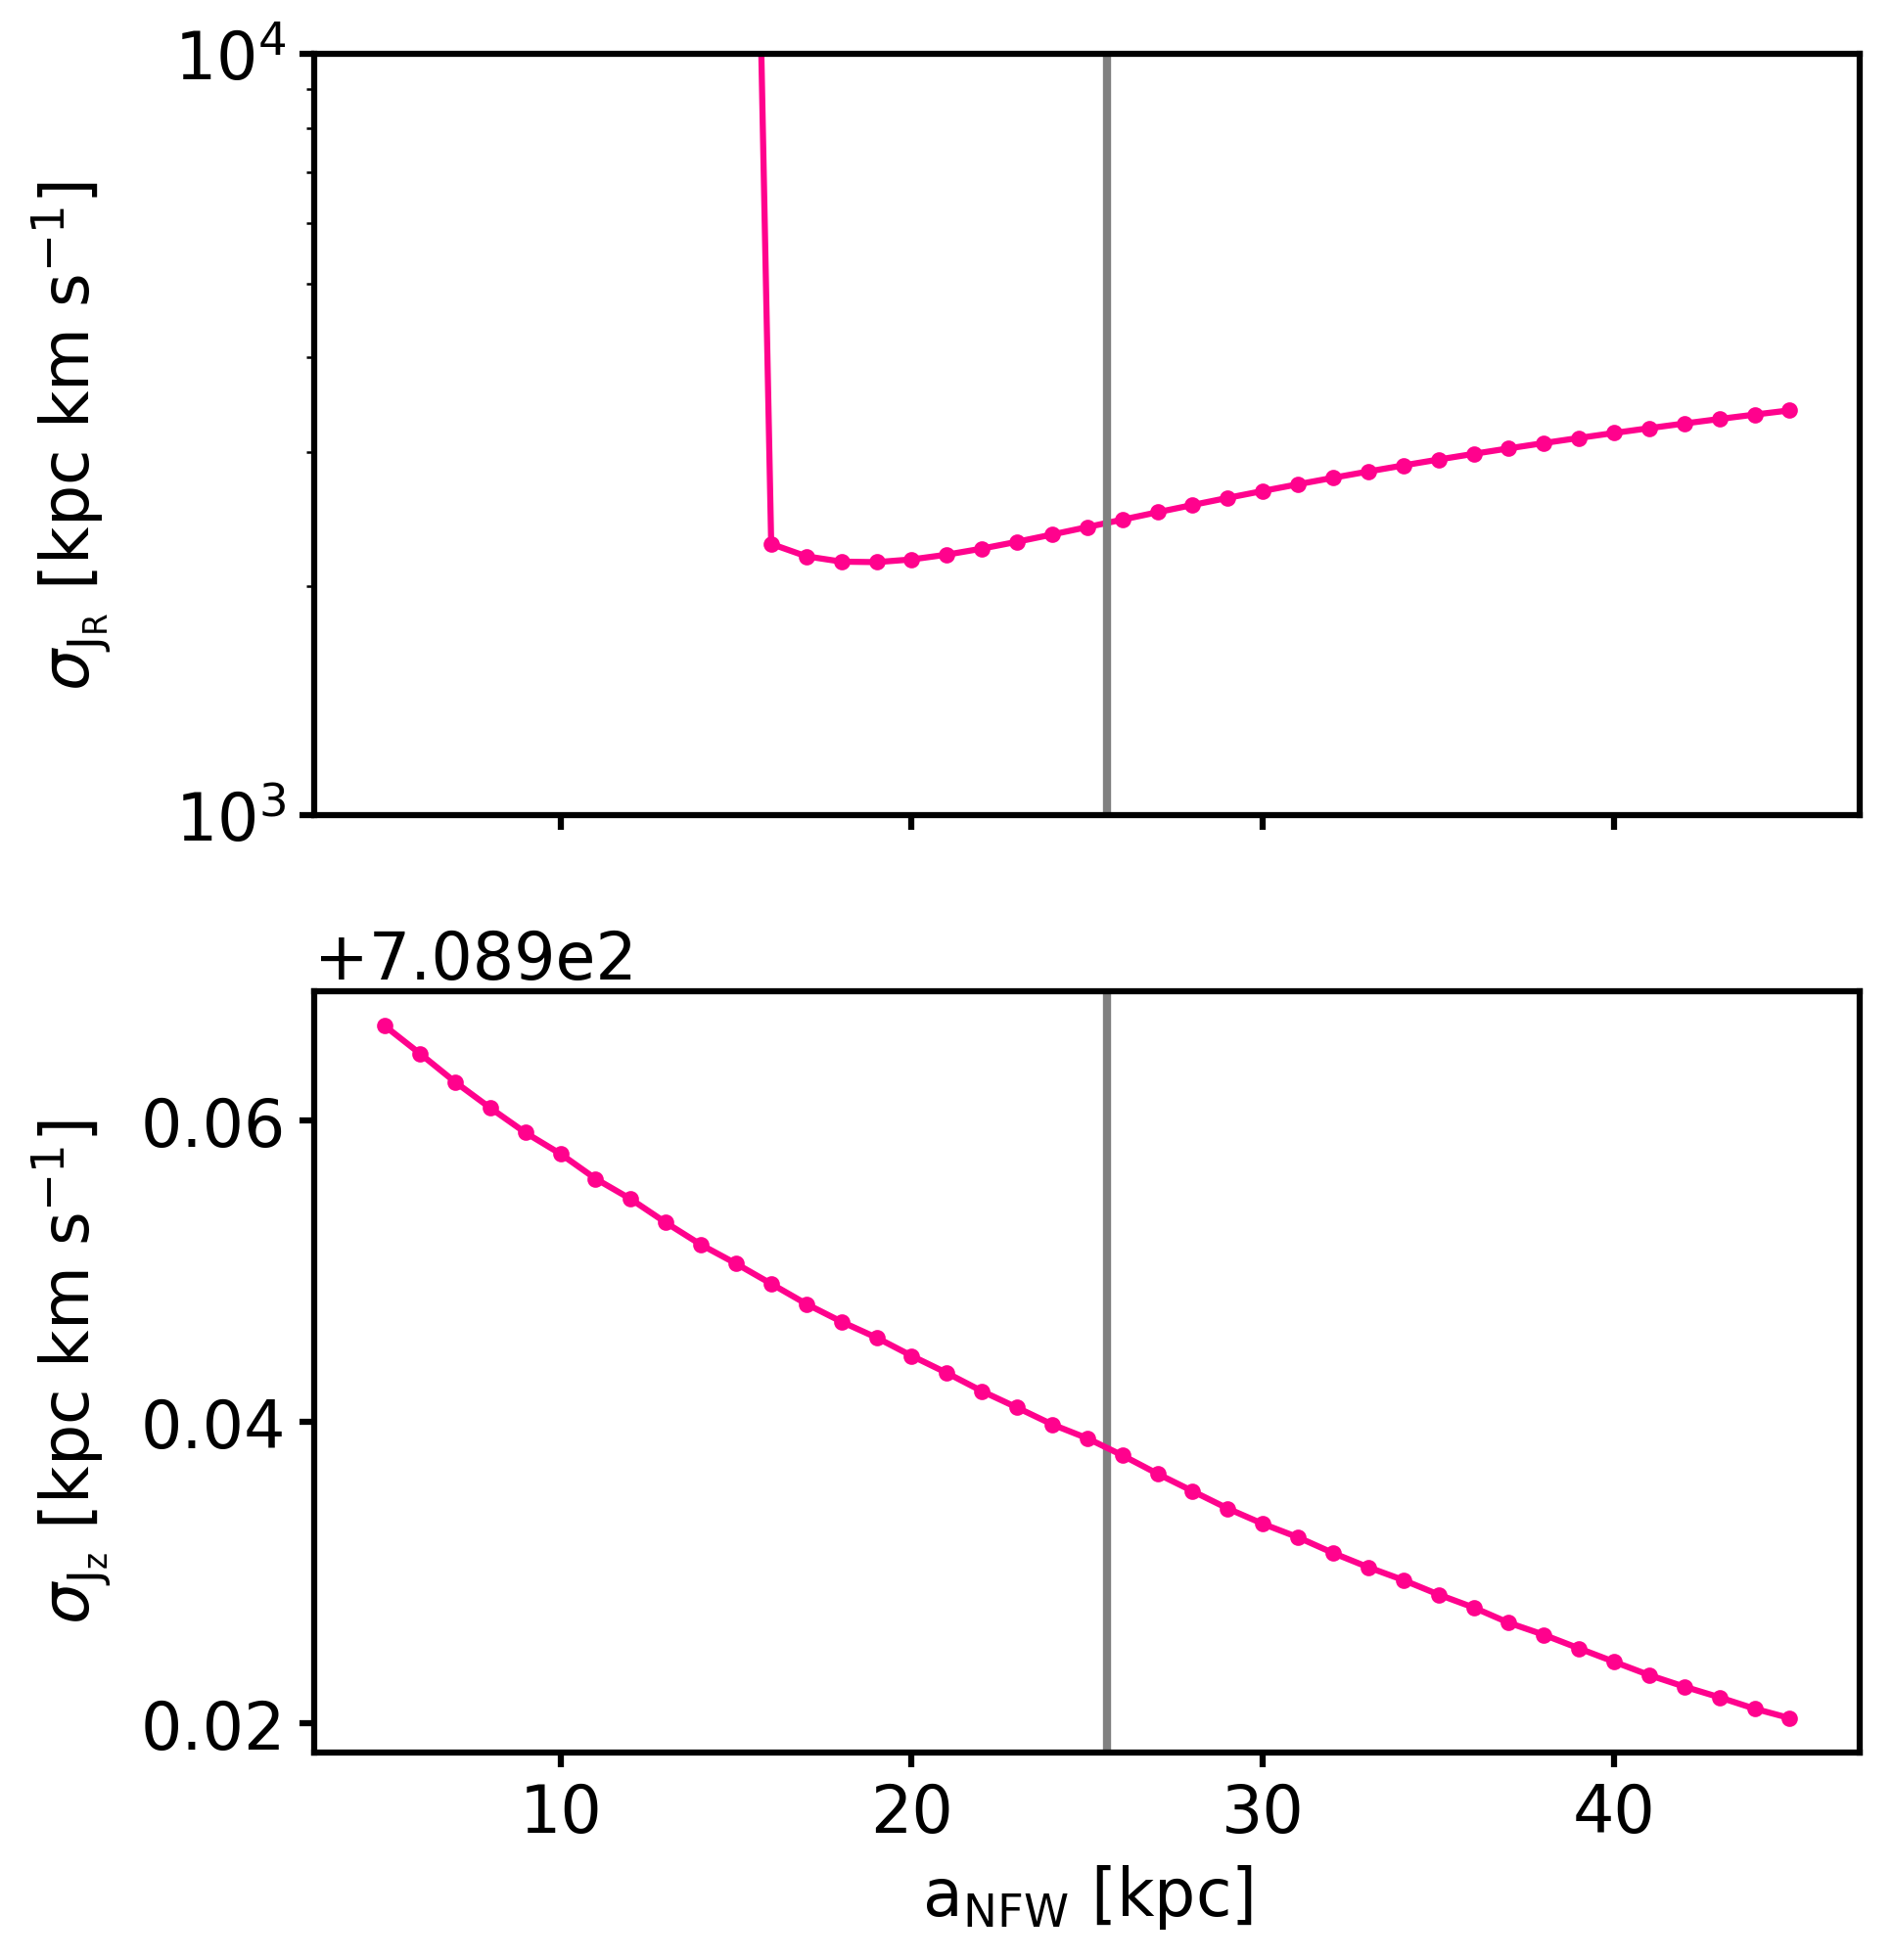
\includegraphics[width=0.48\textwidth]{plots/Dynamics/prog2/a_NFW_diagnostic_plot_std_prog2_all.png}}\hfill%
   \subfloat{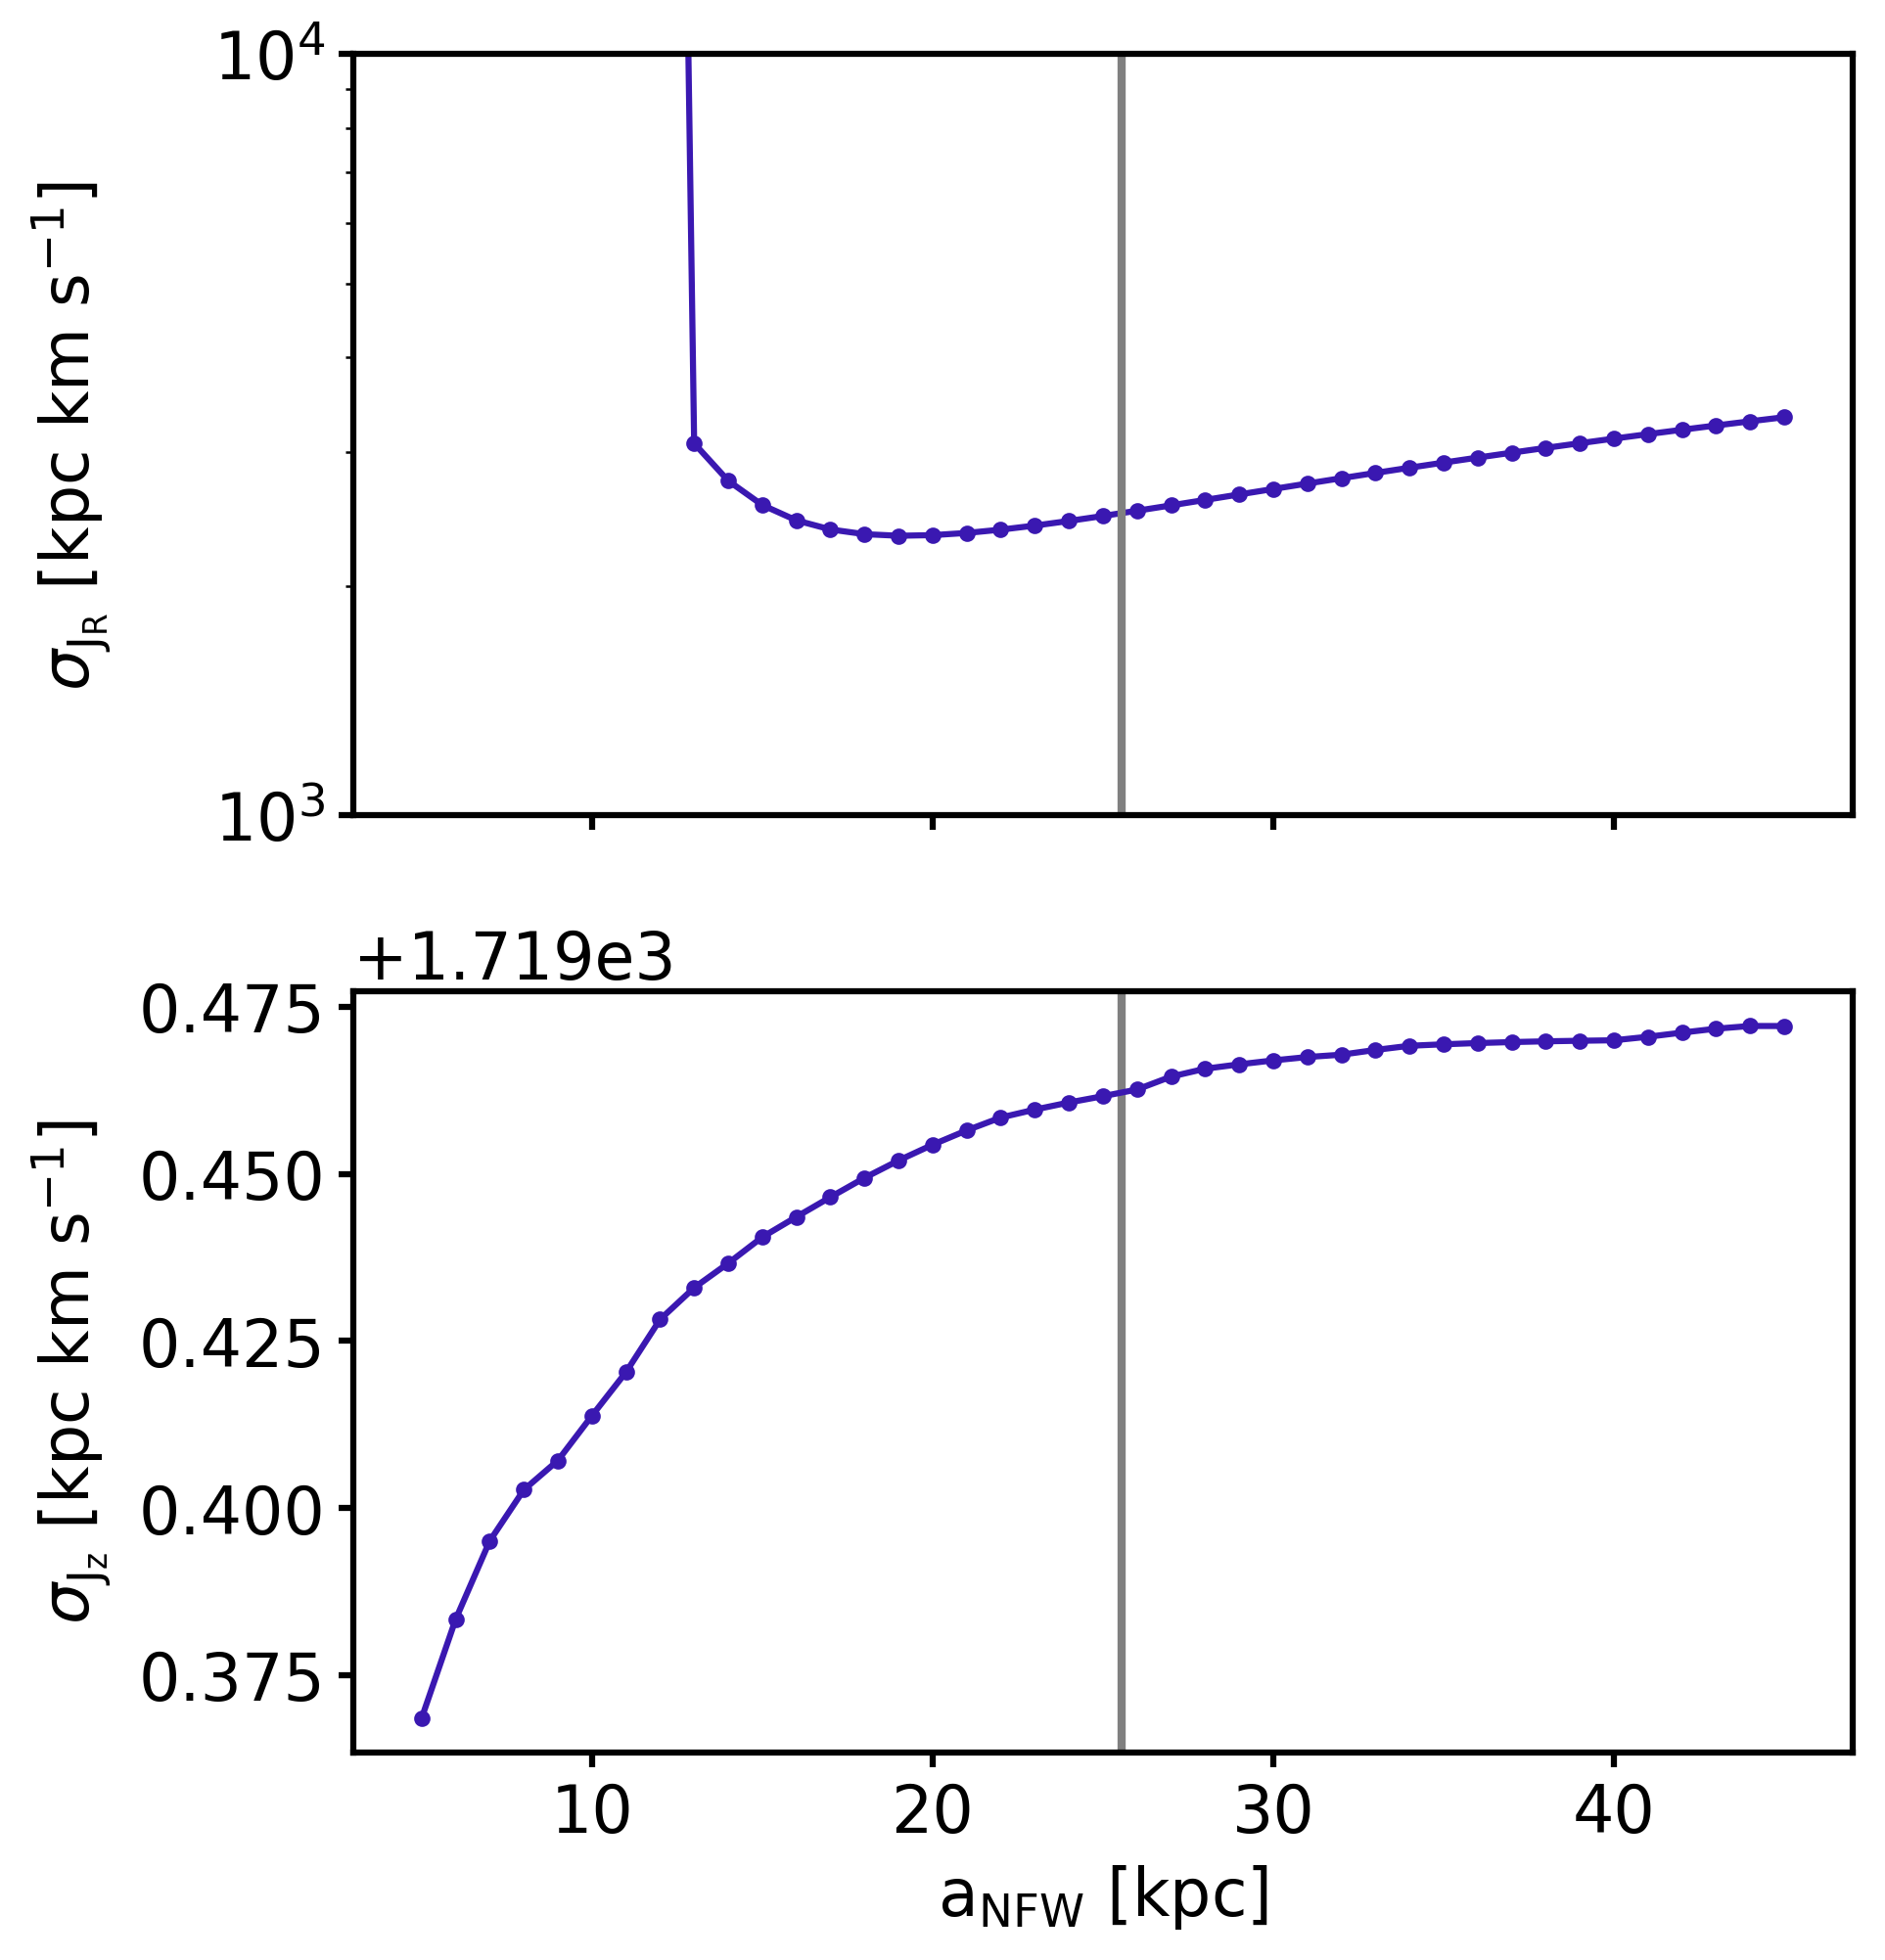
\includegraphics[width=0.48\textwidth]{plots/Dynamics/prog3/a_NFW_diagnostic_plot_std_prog3_all.png}}\vspace*{0.5cm}\par
   \subfloat{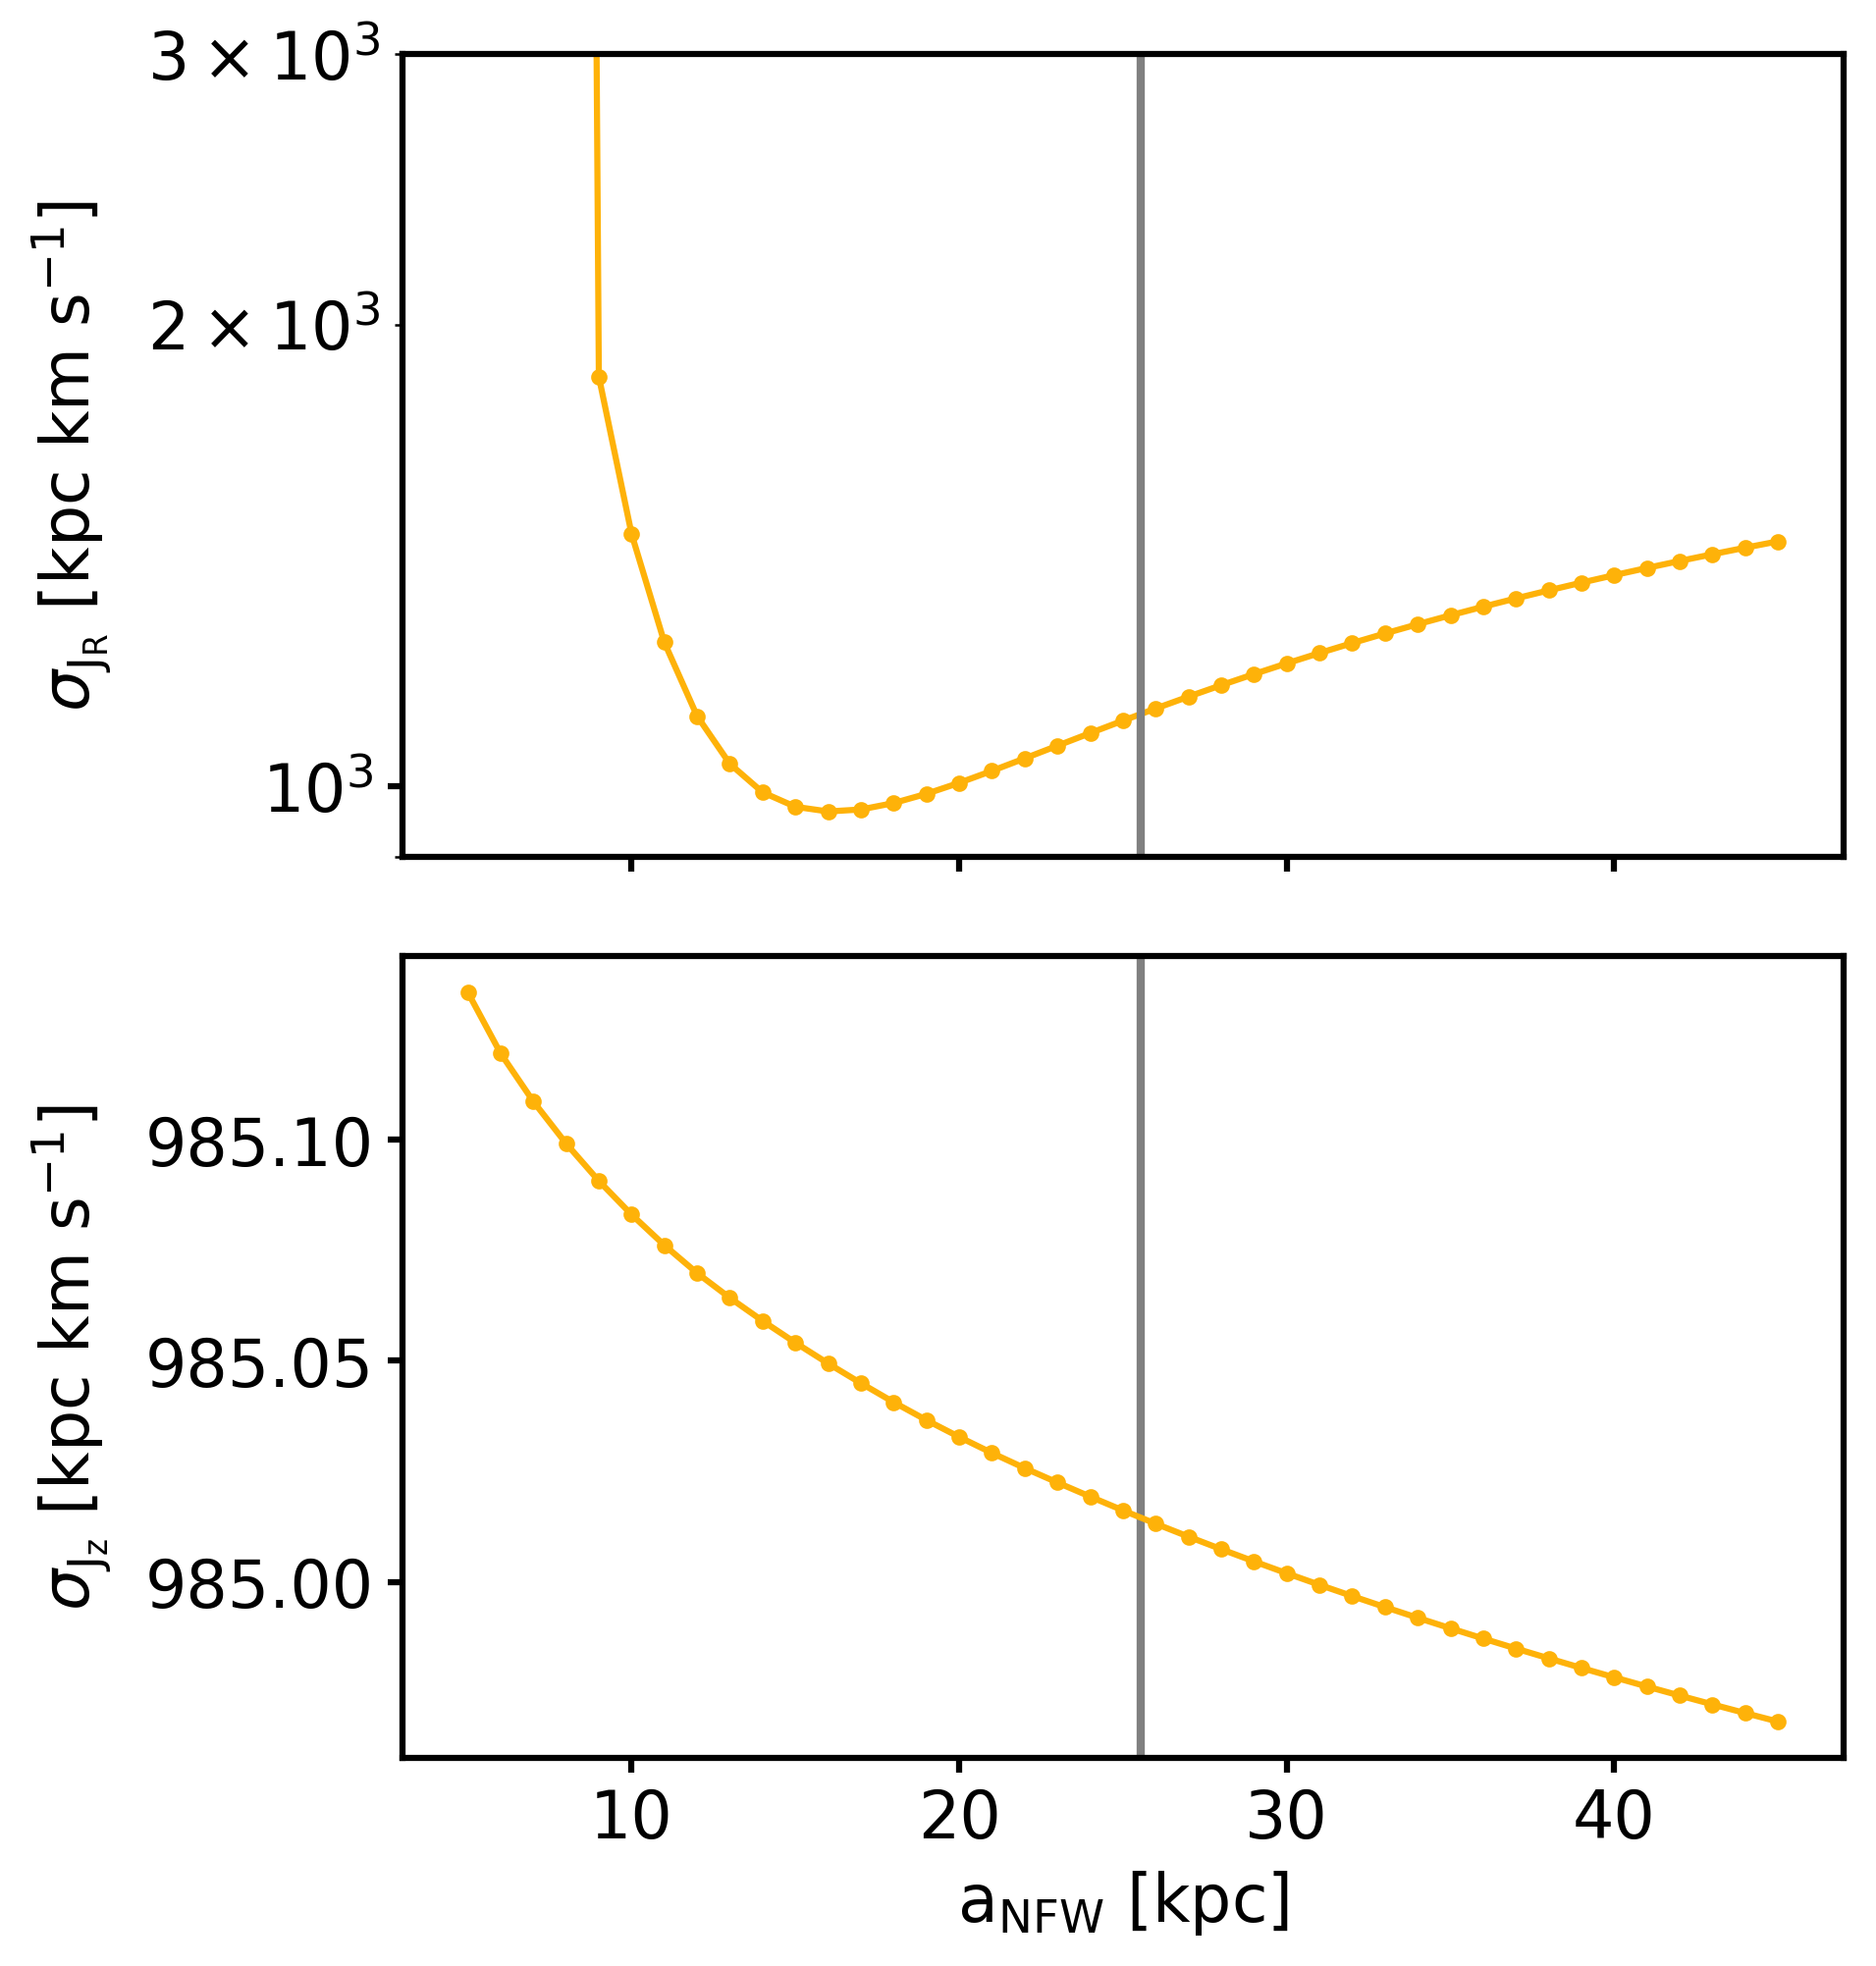
\includegraphics[width=0.48\textwidth]{plots/Dynamics/prog4/a_NFW_diagnostic_plot_std_prog4_all.png}}\hfill%
   \parbox[b][.3\textheight]{.48\textwidth}%
     {\vskip-\abovecaptionskip\RawCaption{\caption{Standard deviations of the radial and vertical actions of all three mergers (prog2-pink / prog3-blue / prog4-yellow) in potentials with varying scale length of the \ac{DM} halo and all other parameters kept on their best fit value. We would expect the standard deviation to be mimized at the best fit potential which is indicated with the vertical grey line. We see that the radial action would prefer a lower scale length (at \SI{17}{kpc}) while two of the three vertical actions would prefer higher scale lengths. The differences in $\sigma_{J_z}$ are much smaller than the one in $\sigma_{J_R}$. \textcolor{red}{update with new selected GCs coming}}\vfill\label{fig:a_NFW_diagnostic_plots}}}
\end{figure}
In Figure \ref{fig:a_NFW_diagnostic_plots}, we see how the standard deviations of the radial and vertical actions evolve in the different potentials. For all three \acp{GC} groups we see that in the radial action they would prefer a smaller scale length of the halo potential. The changes in vertical action are very small but two of three groups would prefer a larger scale length. 
\\\\This leads us to the conclusion that in the "true" potential, accreted \acp{GC} of one \ac{DG} are not on similar orbits but have a \ac{DF} that is more complex. We cannot constrain an analytic axisymmetric gravitational potential by only minimizing the spread of these \acp{GC} in action space.

\subsection{Time evolution of actions}\label{subsec:time_evo_actions}
We evaluate the time evolution of the orbits of the accreted \acp{GC} to see if there was a point - probably shortly after their mergers - where the \acp{GC} were more clumped in action space and the \ac{DF} could have been a $\delta$-function. If that would be true, we could at least determine the potential of galaxies which are in a state shortly after a minor merger. We calculate the actions of the selected particles in the best fit potential in each snapshot.  

\subsubsection{Best fit potential}\label{subsubsec:GCs_action_time_right_pot}
With the method described in Section \ref{subsec:best_fit_pot} we fit an analytic axisymmetric potential to each snapshot individually and interpolate the parameters for a smooth potential evolution (see Figure \ref{tab:pot_best_fit_params}). We trace back the \acp{GC} we considered as merged and calculate their actions in each snapshot for both after and before the merger. 
\begin{figure}[htbp]
\captionsetup{format=plain}
    \centering
	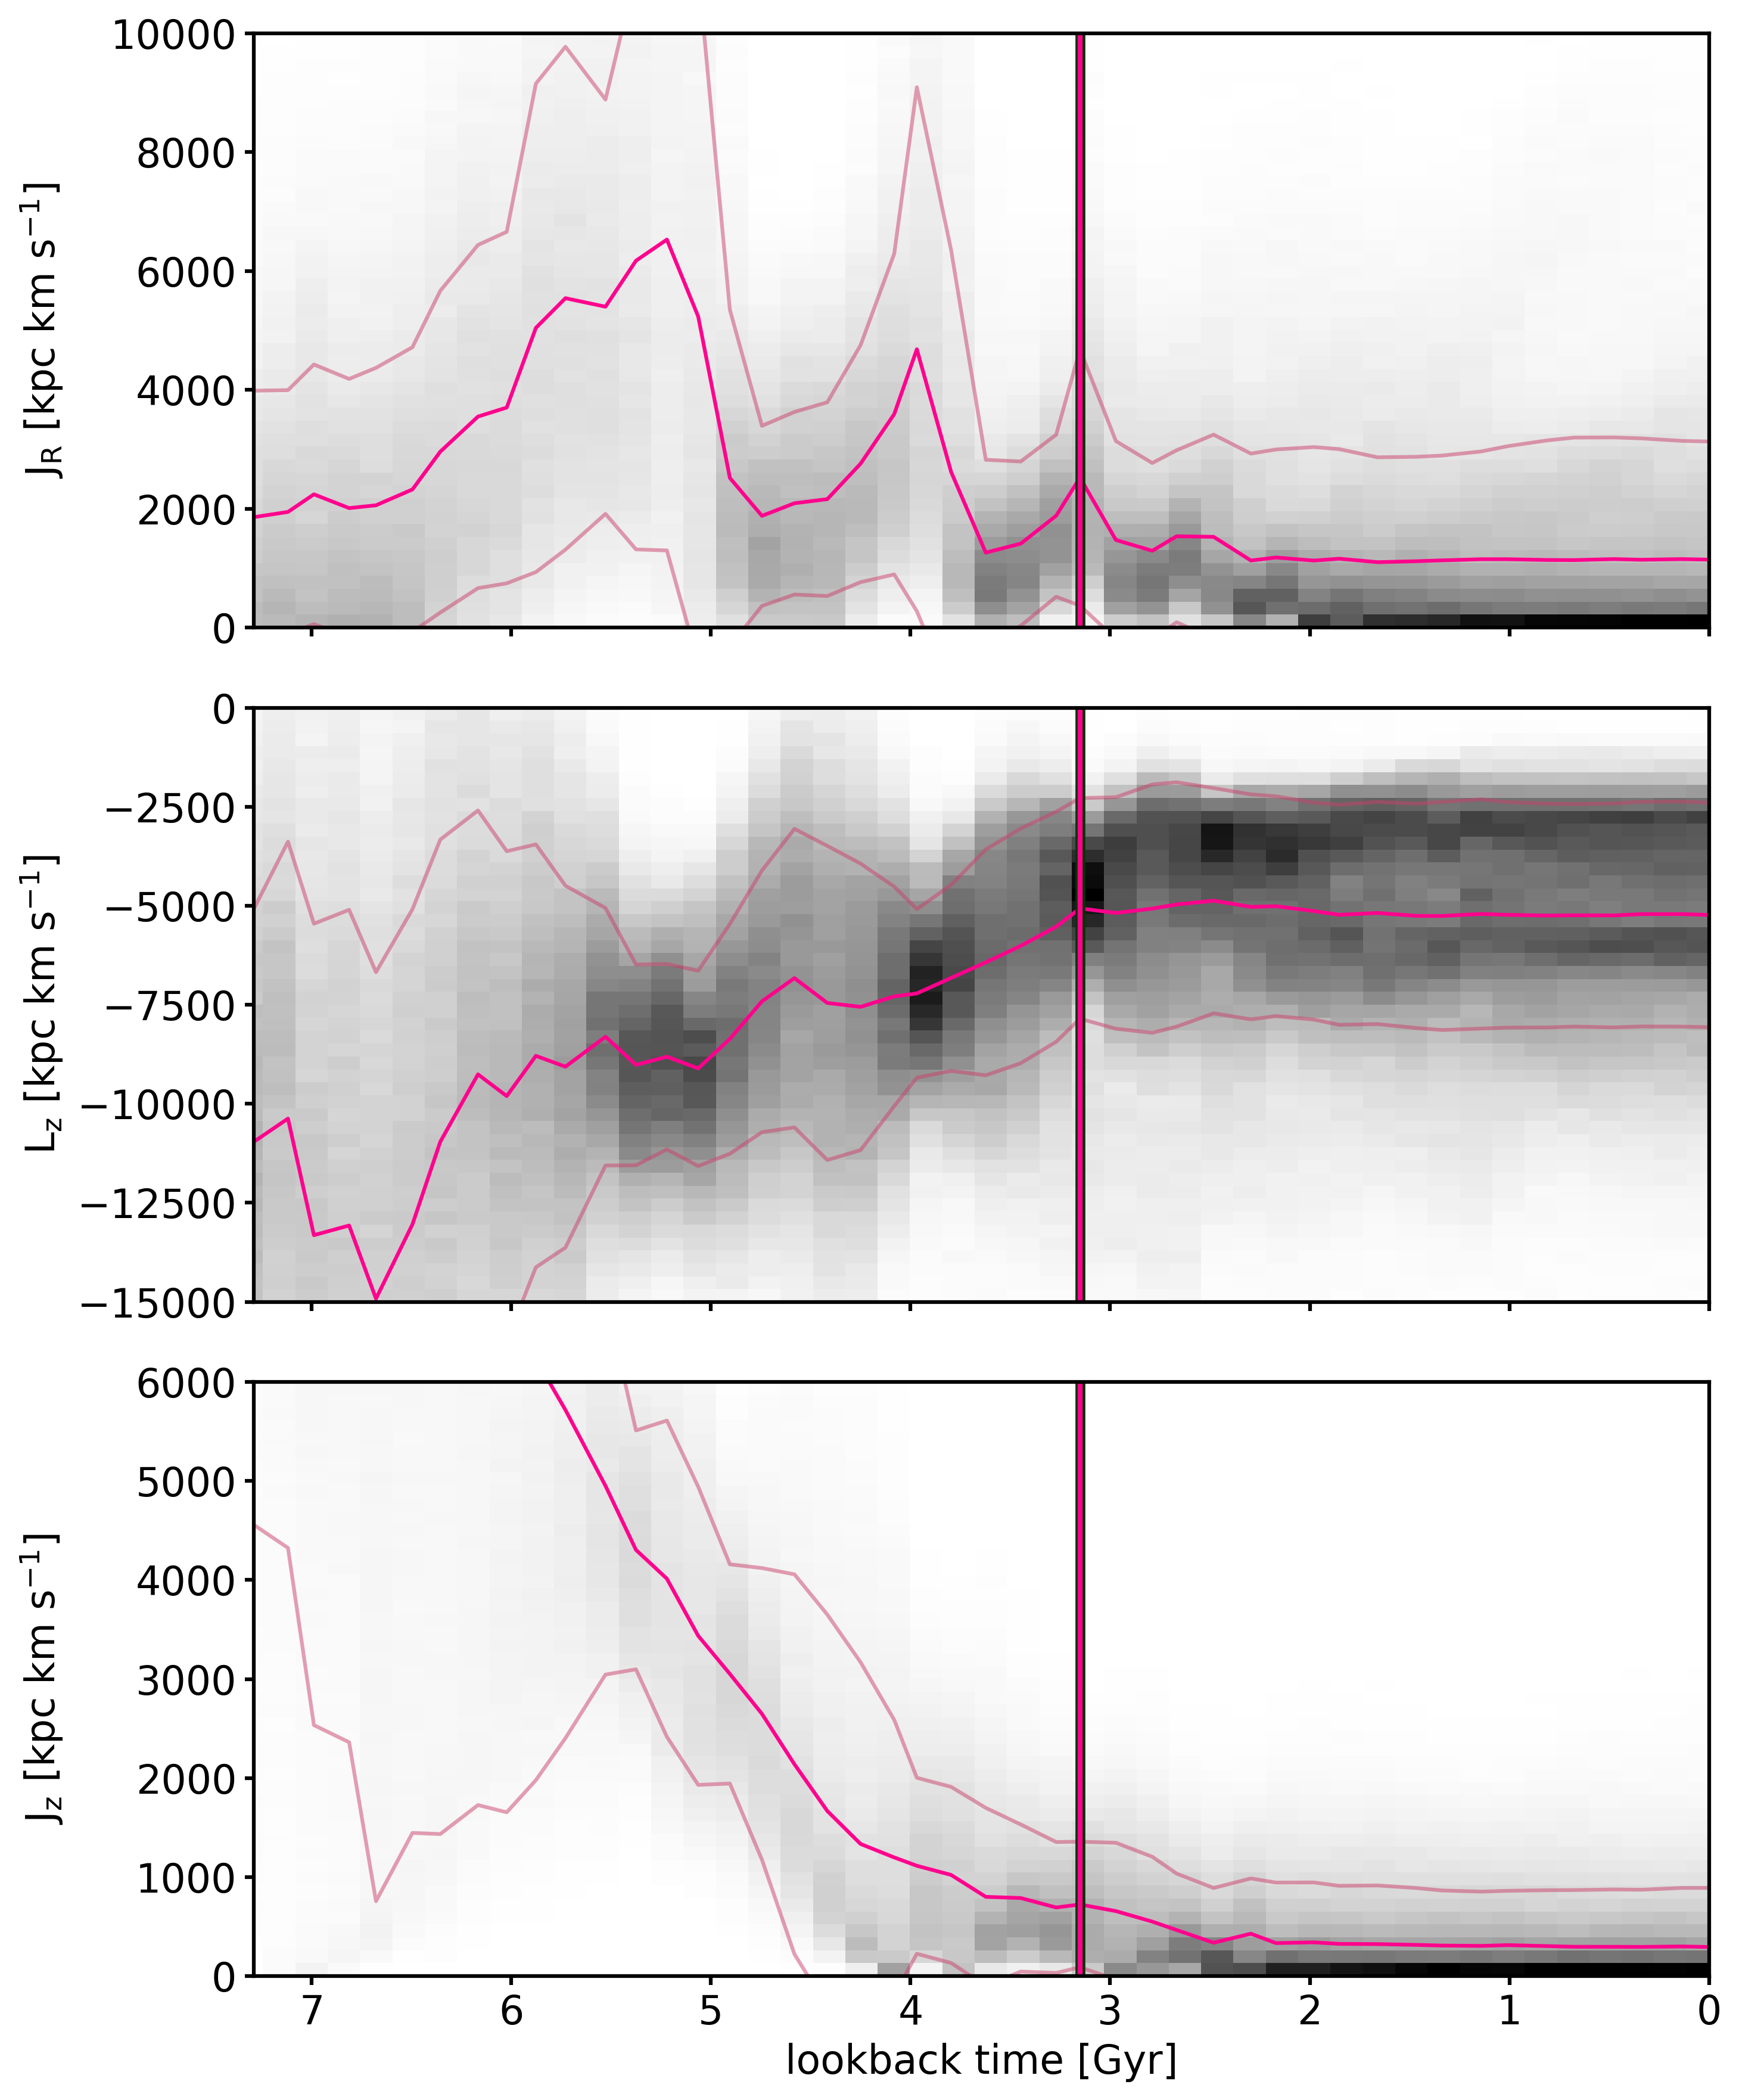
\includegraphics[width=\textwidth]{plots/Dynamics/prog2/action_time_evolution_wodisk_hist_mean.png}

	\caption{Evolution of actions of prog2 \acp{GC} over time. The pink vertical line indicates the time of the merger. The other pink lines follow the median (bright pink) and the standard deviation (light pink). \textit{Upper panel}: Radial action. \textit{Middle panel}: Angular momentum. \textit{Lower panel}: Vertical action. Before the merger, radial and vertical action were much higher and all three actions had higher standard deviations. This indicates that their motions were not yet governed by our main galaxy's potential. With the merger, they have settled and $L_z$ and $J_z$ have a constant mean and standard deviation. $J_R$ has a small median and standard deviation shortly before the merger but since then both have increased again.}\label{fig:actions_time_evolution_prog2}
\end{figure}

\begin{figure}
\captionsetup{format=plain}
    \centering
	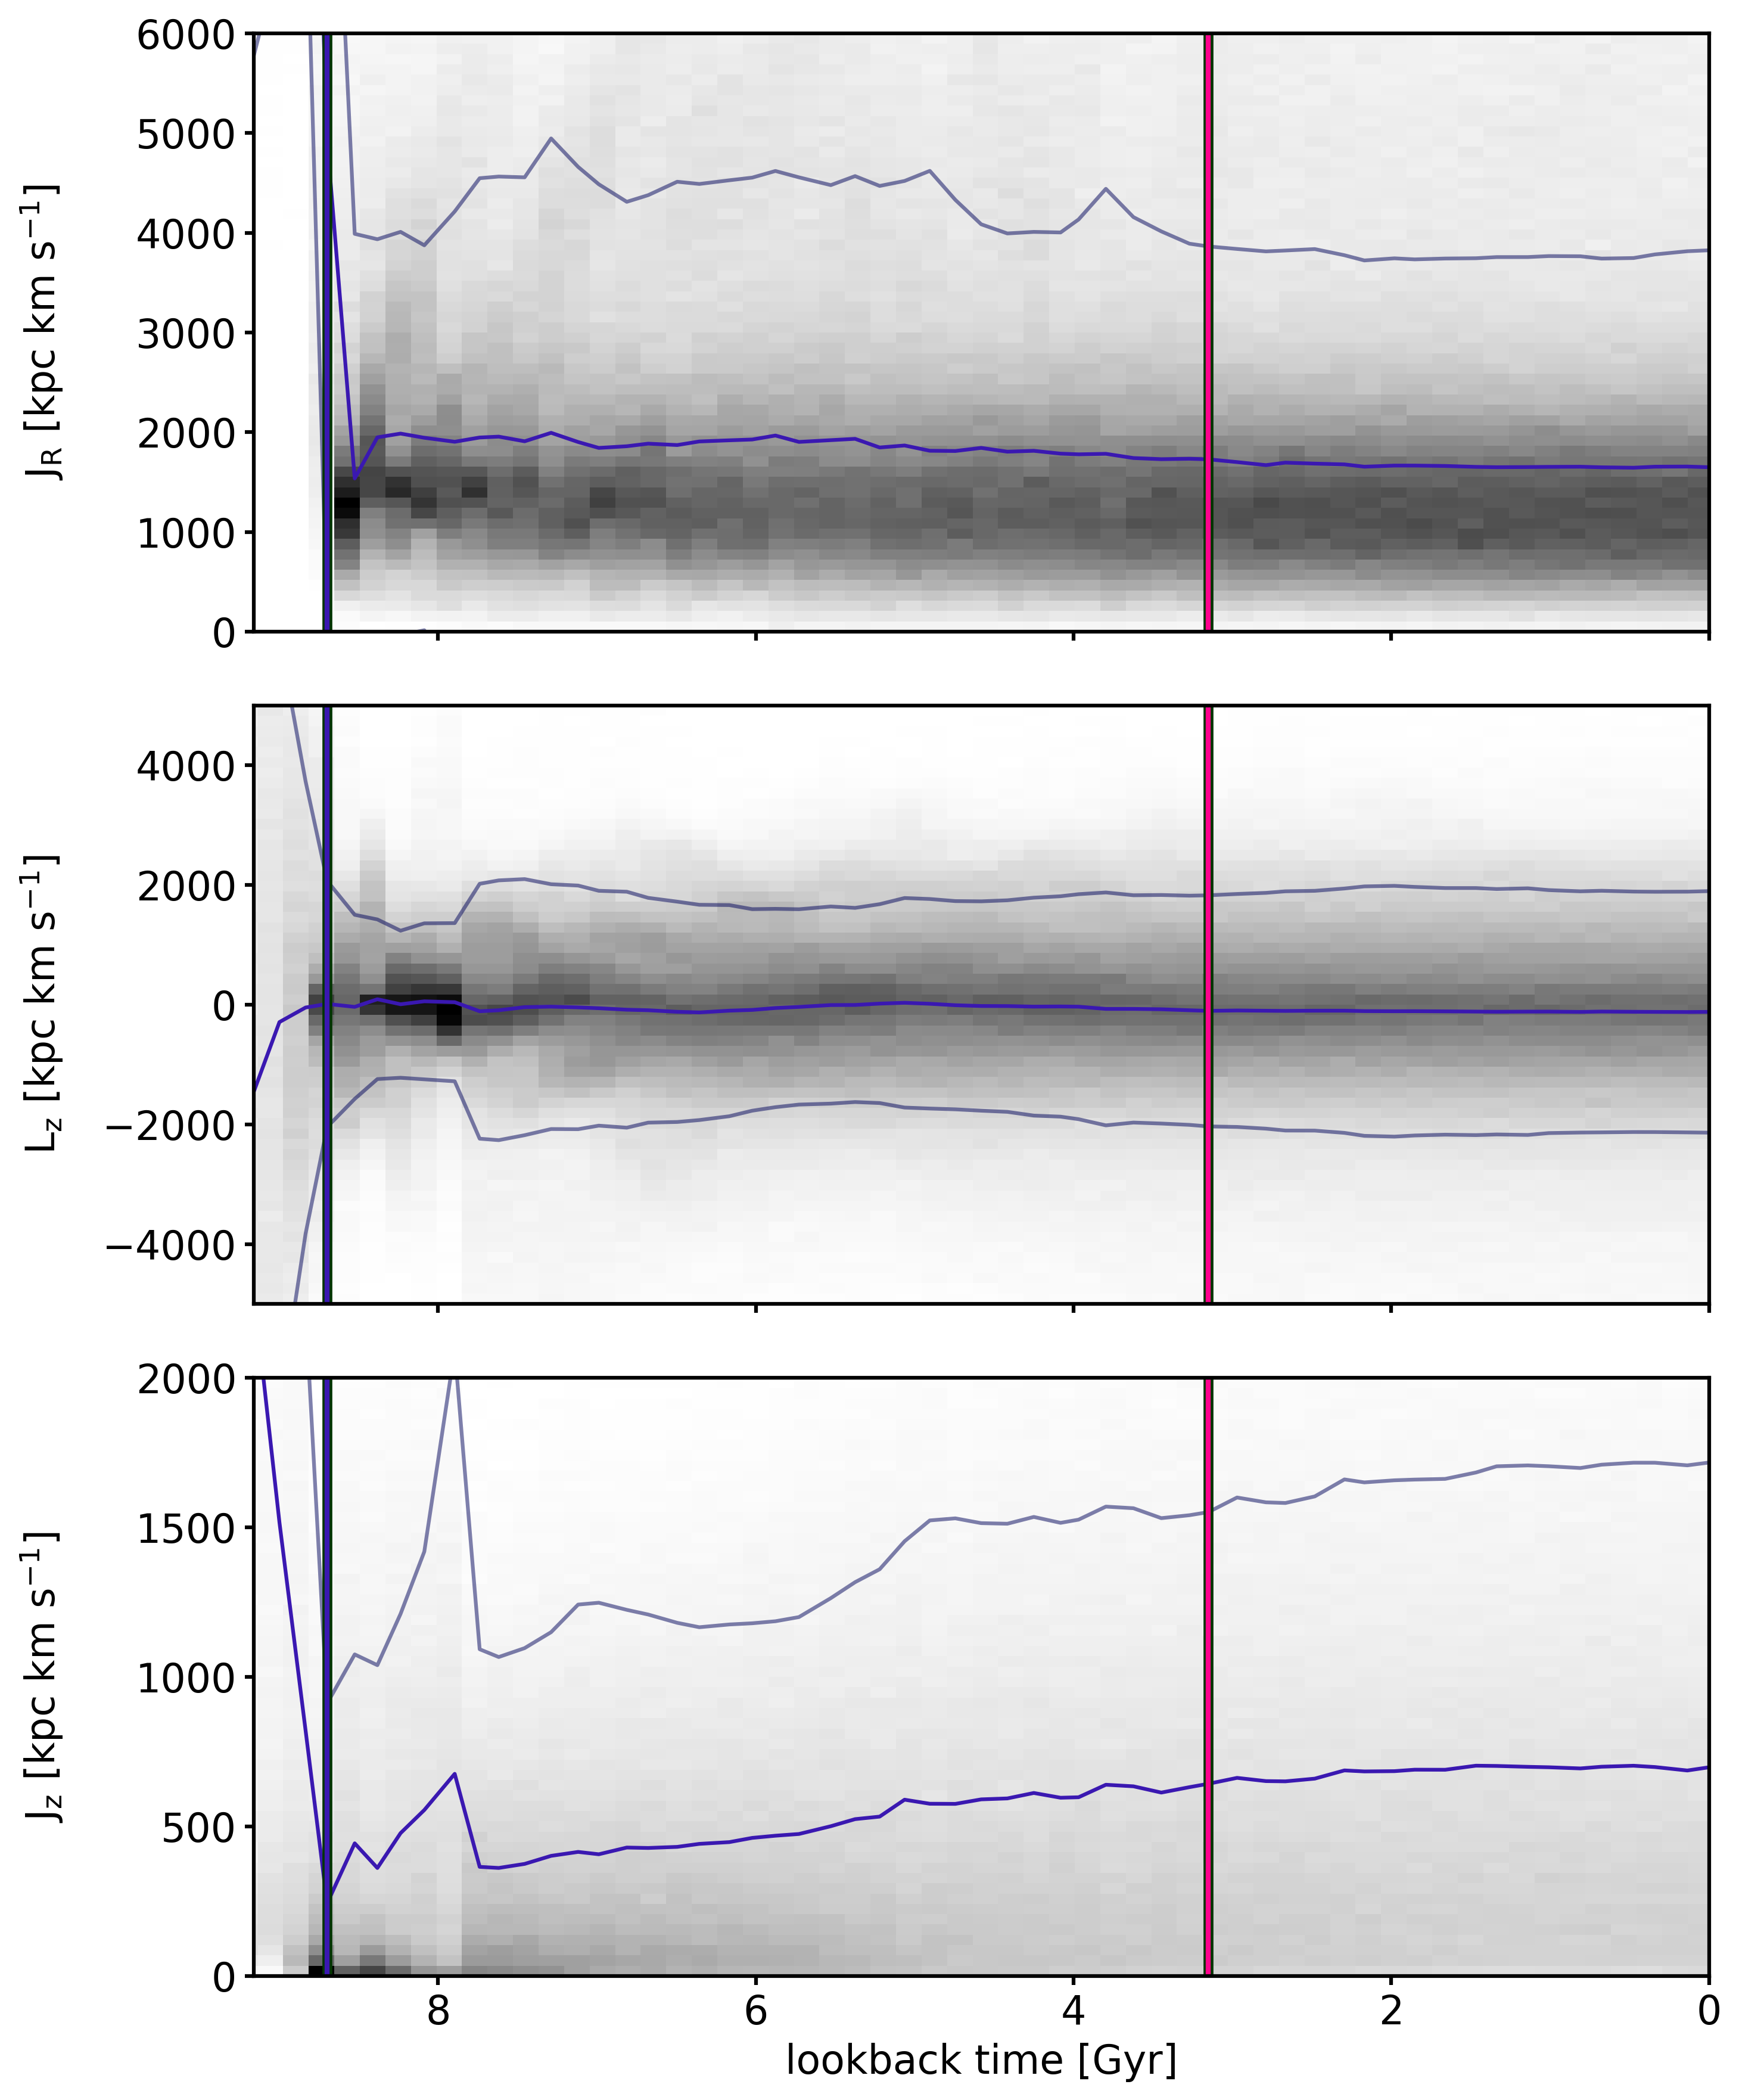
\includegraphics[width=\textwidth]{plots/Dynamics/prog3/action_time_evolution_wodisk_hist_mean.png}
    \caption{Time evolution of actions of prog3. The vertical pink and blue lines indicate times of the mergers of prog2 and prog3, respectively. The other blue lines are the median and the standard deviation. The panels are the same as in Figure \ref{fig:actions_time_evolution_prog2}. During the merger of prog3, $\overline{J}_z$ and $\sigma{_J_z}$ minimize. \textcolor{red}{explain what happens with the potential at that point}Shortly after the merger, the spread in $J_R$ and in $L_z$ minimizes while at the same time the median of $J_z$ and $\sigma{_J_z}$ rise steeply. The following evolution is rather constant for all actions with the spread slowly increasing.}\label{fig:actions_time_evolution_prog3}
\end{figure}

\begin{figure}[htbp]
\captionsetup{format=plain}
    \centering
	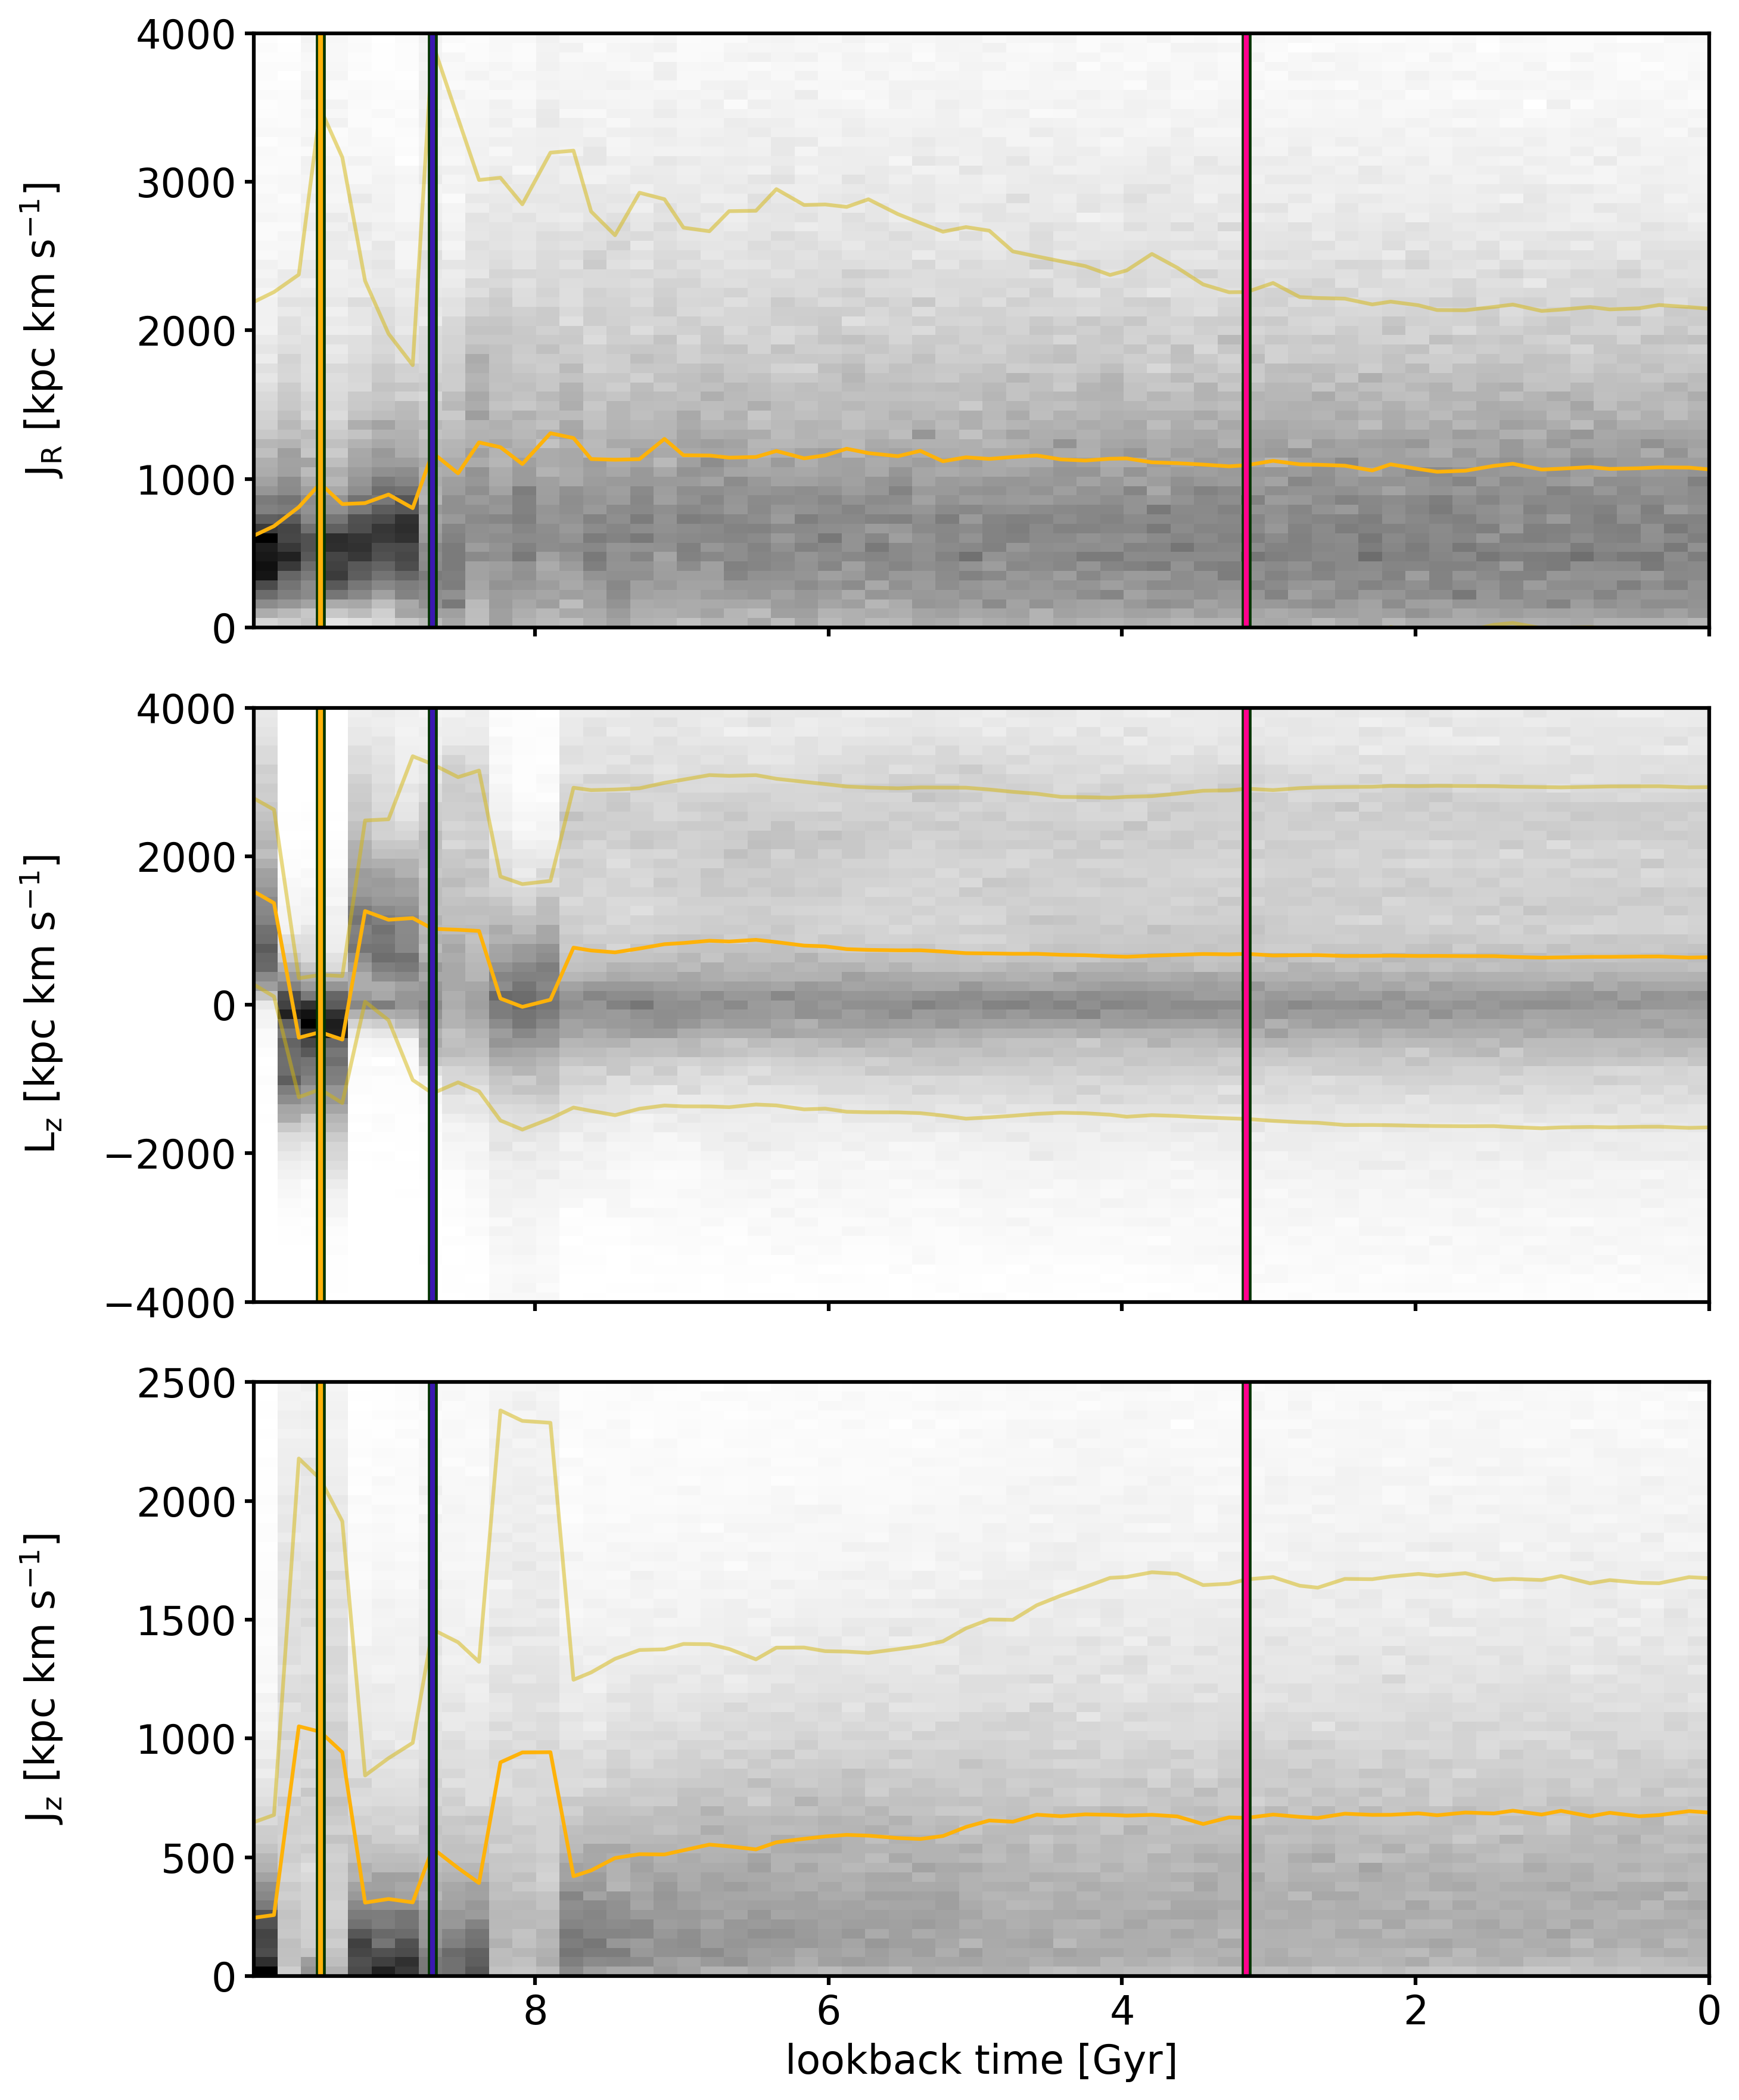
\includegraphics[width=\textwidth]{plots/Dynamics/prog4/action_time_evolution_wodisk_hist_mean.png}
    \caption{Prog4's \acp{GC} time evolution in action space. The vertical pink, blue and yellow lines indicate times of the mergers of prog2, prog3 and prog4, respectively. The yellow lines are median and standard deviation. The panels are the same as in Figure \ref{fig:actions_time_evolution_prog2}. \textcolor{red}{Check that description is still valid} During the merger of prog4, radial and vertical actions have a steep rise while $L_z$ drops below 0. Something similar happens shortly after the merger of prog3. Since \SI{7.5}{Gyr} the actions stay constant and with the merger of prog2, the scatter in $J_R$ and $J_z$ becomes even less, is, however, still very large.}\label{fig:actions_time_evolution_prog4}
\end{figure}
In Figures \ref{fig:actions_time_evolution_prog2}, \ref{fig:actions_time_evolution_prog3} and \ref{fig:actions_time_evolution_prog4} we present these time evolutions for the \acp{GC} of prog2 / prog3 / prog4, respectively. For the prog2 \acp{GC}, Figure \ref{fig:actions_time_evolution_prog2}, we see nicely how before the merger the actions where very widely spread and towards the merger and especially afterwards their variance becomes smaller and the mean of each action stays constant. Since the merger, more significant clumping than in the last snapshot is not seen. In prog3, we find a strong clump shortly after the merger. The actions of prog4 are strongly varying shortly after the merger for about \SI{2}{Gyr} before they become steady.

\subsubsection{Mean best fit potential}\label{subsubsec:GCs_actions_time_mean_right_pot}
The idea that actions do not change over time is valid in a static or only slowly varying (axisymmetric) potential. Even though the overall action distribution did not change too much over time, we will see in Section \ref{subsec:box_GCs} that individual orbits vary drastically over time. Therefore, we need to test if the assumption of having a potential which only varies slowly is true. A rather simple execution is to calculate the action evolution in a static potential and check if it varies from our results. To do so, we calculate the mean of each potential parameter since the last big merger event (prog2). 
\begin{figure}[htbp]
\captionsetup{format=plain}
    \centering
	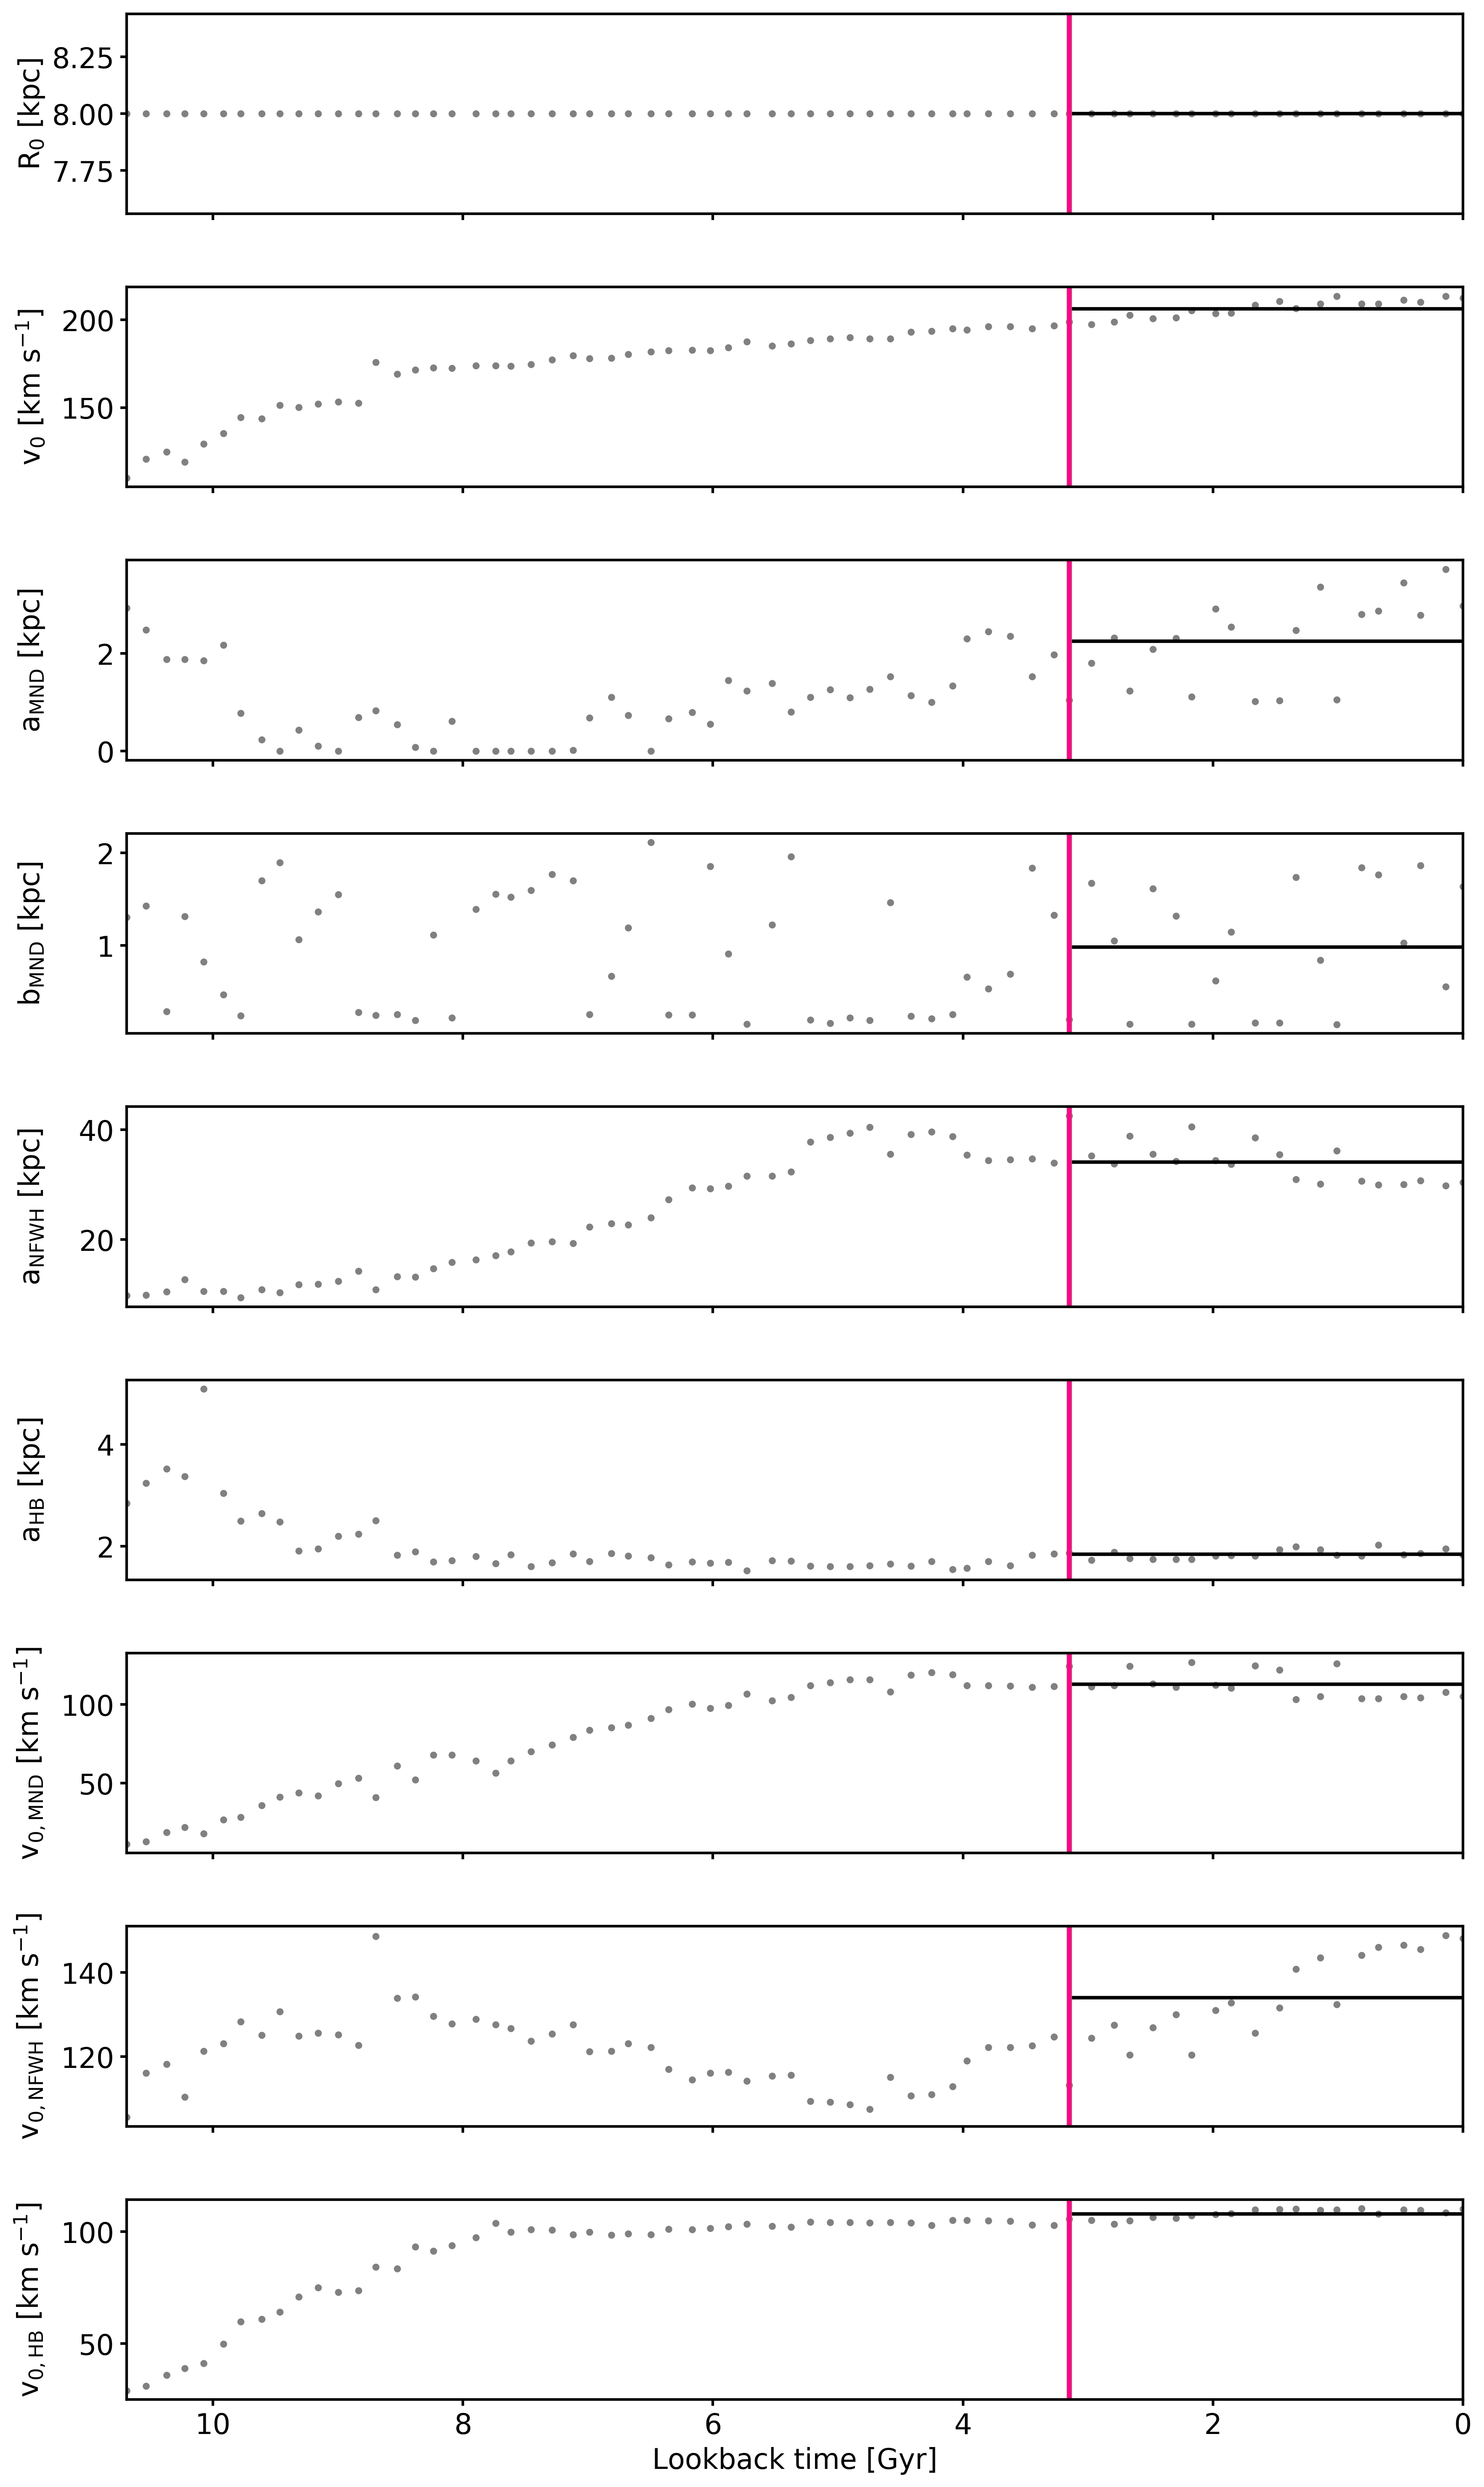
\includegraphics[width=0.8\textwidth]{plots/Dynamics/mean_pot/potential_evolution_with_mean_jan19.png}
    \caption{Time evolution of best fit potential parameters and their mean values since the merger of prog2 (indicated in pink). The scatter of disk and halo parameters is relatively large while the bulge parameters stay constant in this time range. We use the mean potential parameters (indicated as black line) to compare the actions in the slowly varying potential (Figure \ref{fig:pot_val_evol}) to the actions in this static potential.}\label{fig:potential_mean_evolution}
\end{figure}
\\In Figure \ref{fig:potential_mean_evolution}, we show again the parameter evolution and the mean value for each which we use to set up the static gravitational potential. Since we have large scatter in the disk and halo parameters it is interesting to see if ignoring their variation has any consequences on the action calculation. 
\begin{figure}[htbp]
\captionsetup{format=plain}
    \begin{subfigure}[c]{0.48\textwidth}
    \centering
    	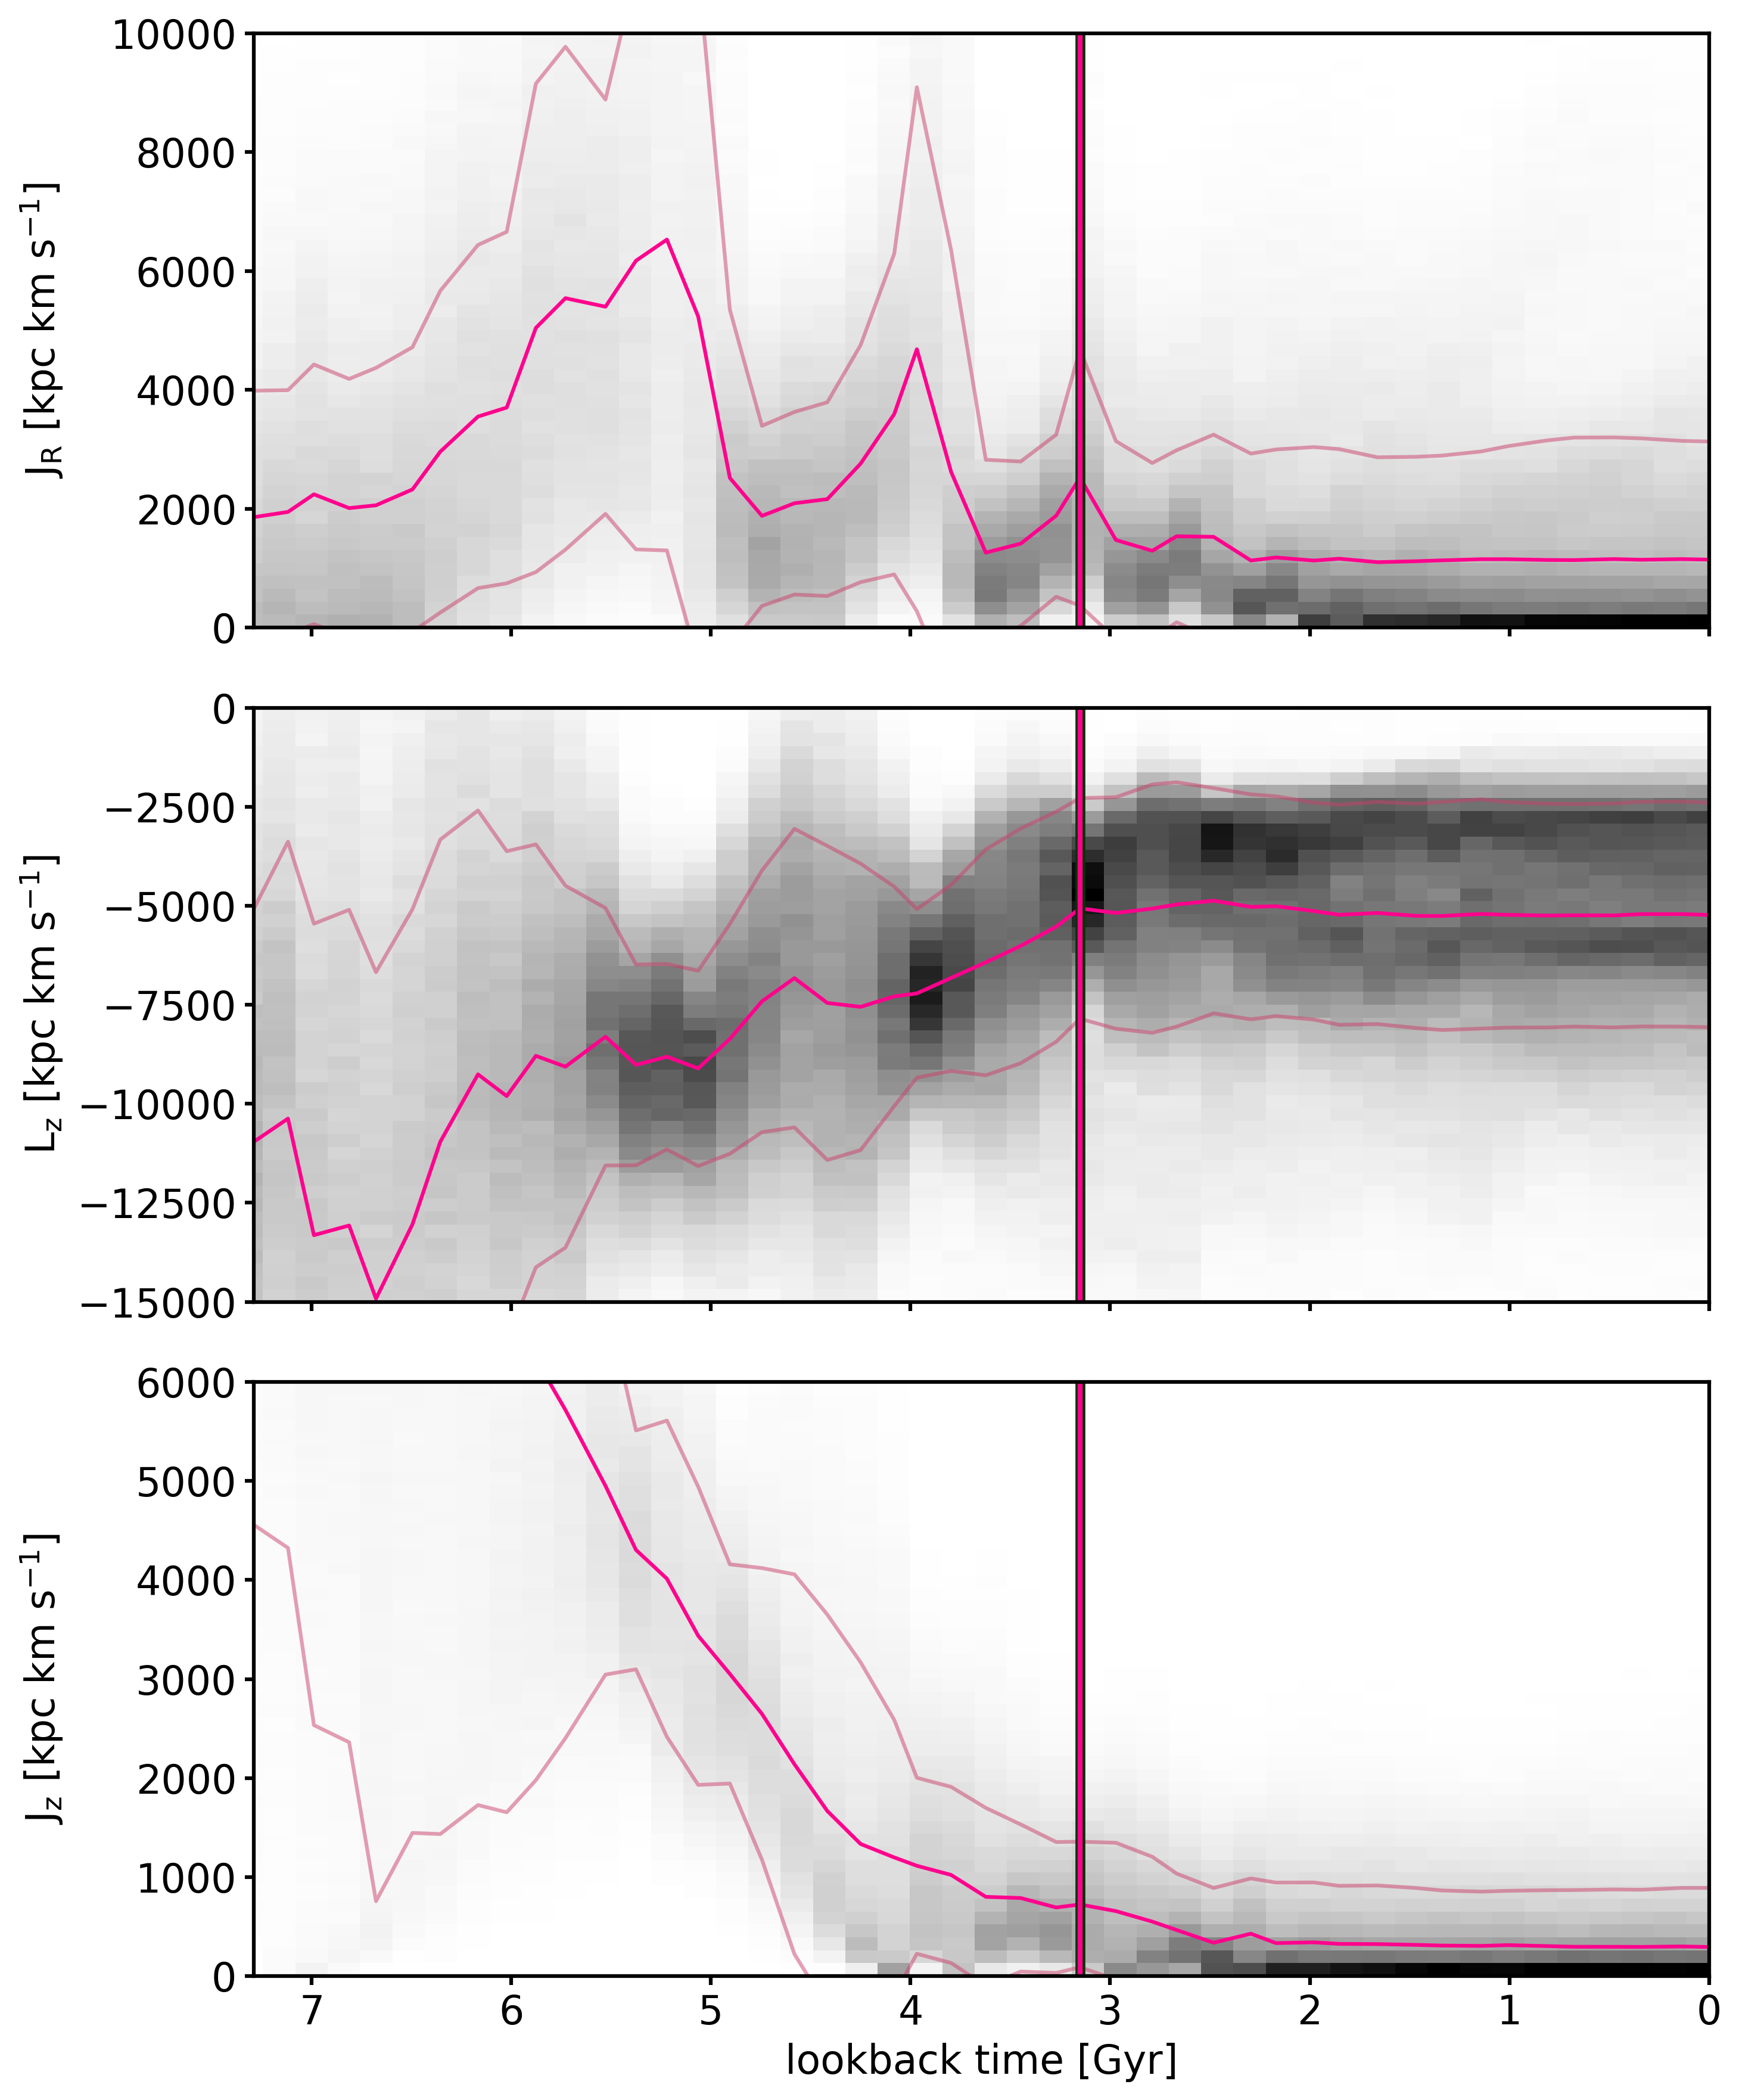
\includegraphics[width=\textwidth]{plots/Dynamics/prog2/action_time_evolution_wodisk_hist_mean.png}
    \end{subfigure}
    ~
    \begin{subfigure}[c]{0.48\textwidth}
    \centering
	    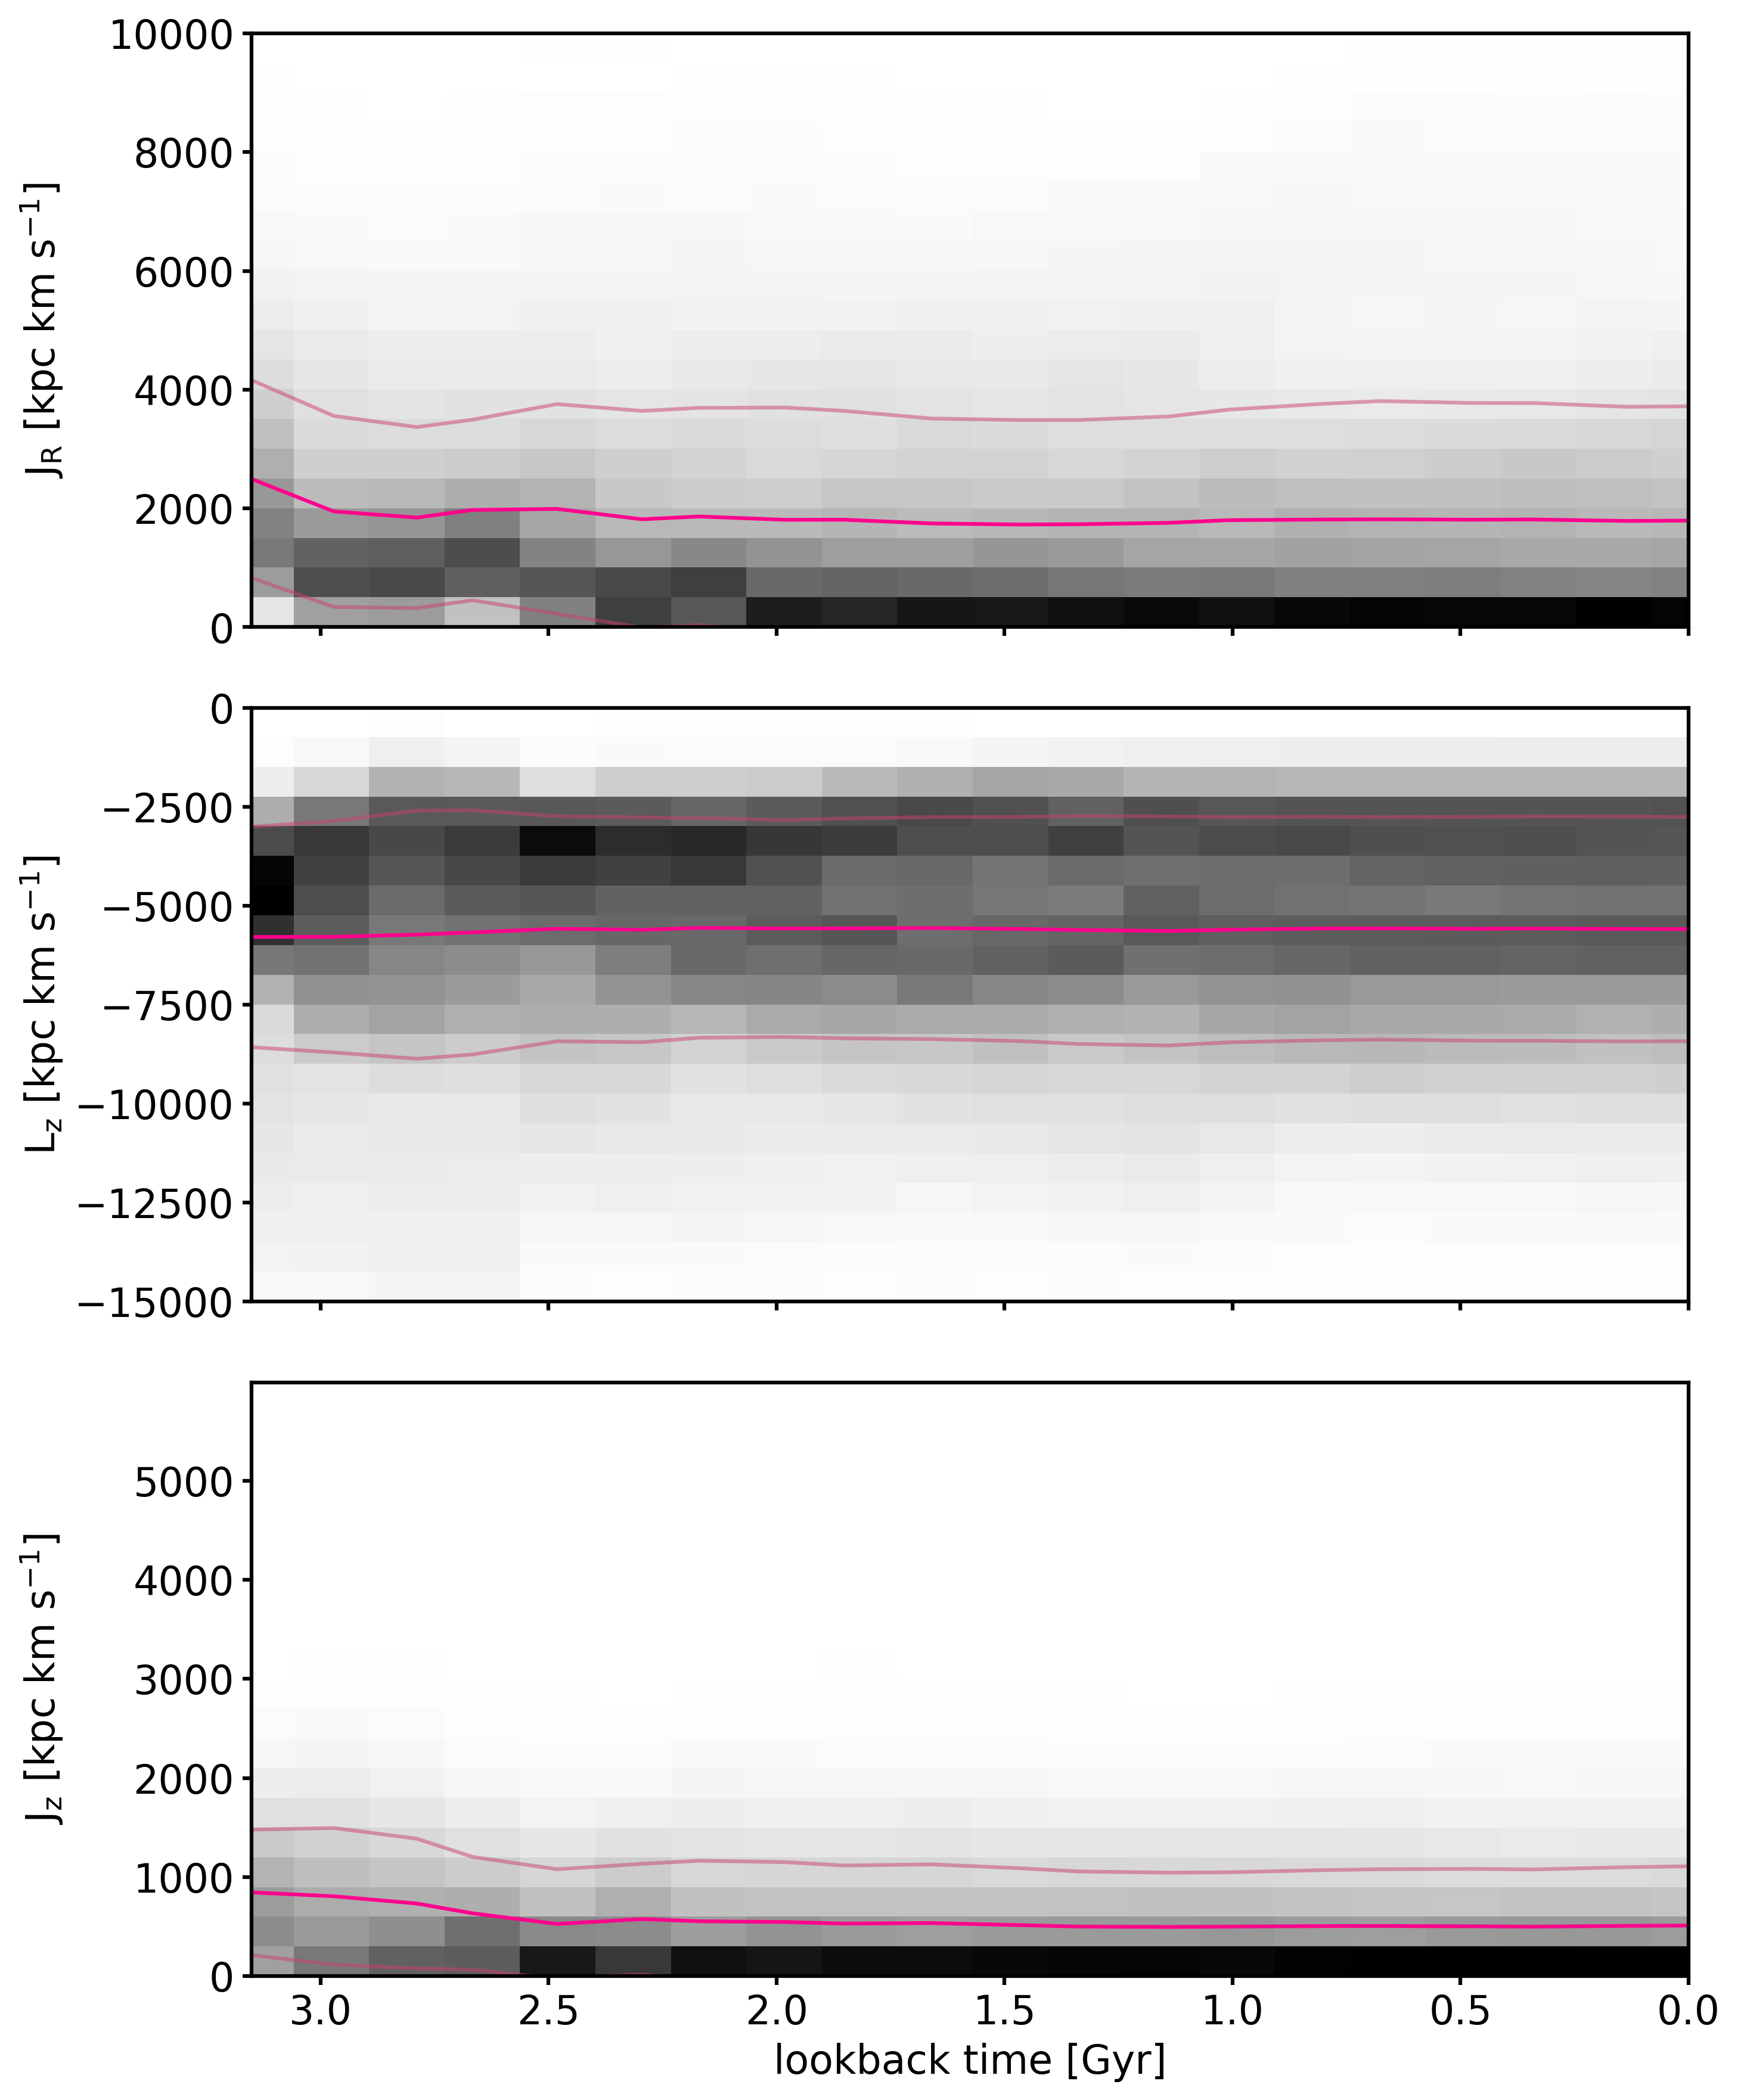
\includegraphics[width=\textwidth]{plots/Dynamics/prog2/action_wodisk_time_evolution_hist_mean_static_pot.png}
    \end{subfigure}
    \caption{Same as Figure \ref{fig:actions_time_evolution_prog2}, only for a constant potential since the merger of prog2.\textcolor{red}{update with new selected GCs coming}}\label{fig:comparison_actions_time_evolution_mean_pot_prog2}
\end{figure}
In the time regime since the last merger we calculated the actions of each progenitor group in the static potential. In Figure \ref{fig:comparison_actions_time_evolution_mean_pot_prog2}, we compare the \acp{GC} of prog2 in action space in the varying potential (left) and the static potential (right). There is no difference in the time evolution visible after the merger. We did the same for the \acp{GC} of prog3 and prog4 and they also show no differences. Therefore, the assumption of having a slowly evolving potential can be considered as satisfied.
\iffalse
\begin{figure}
\captionsetup{format=plain}
    \centering
	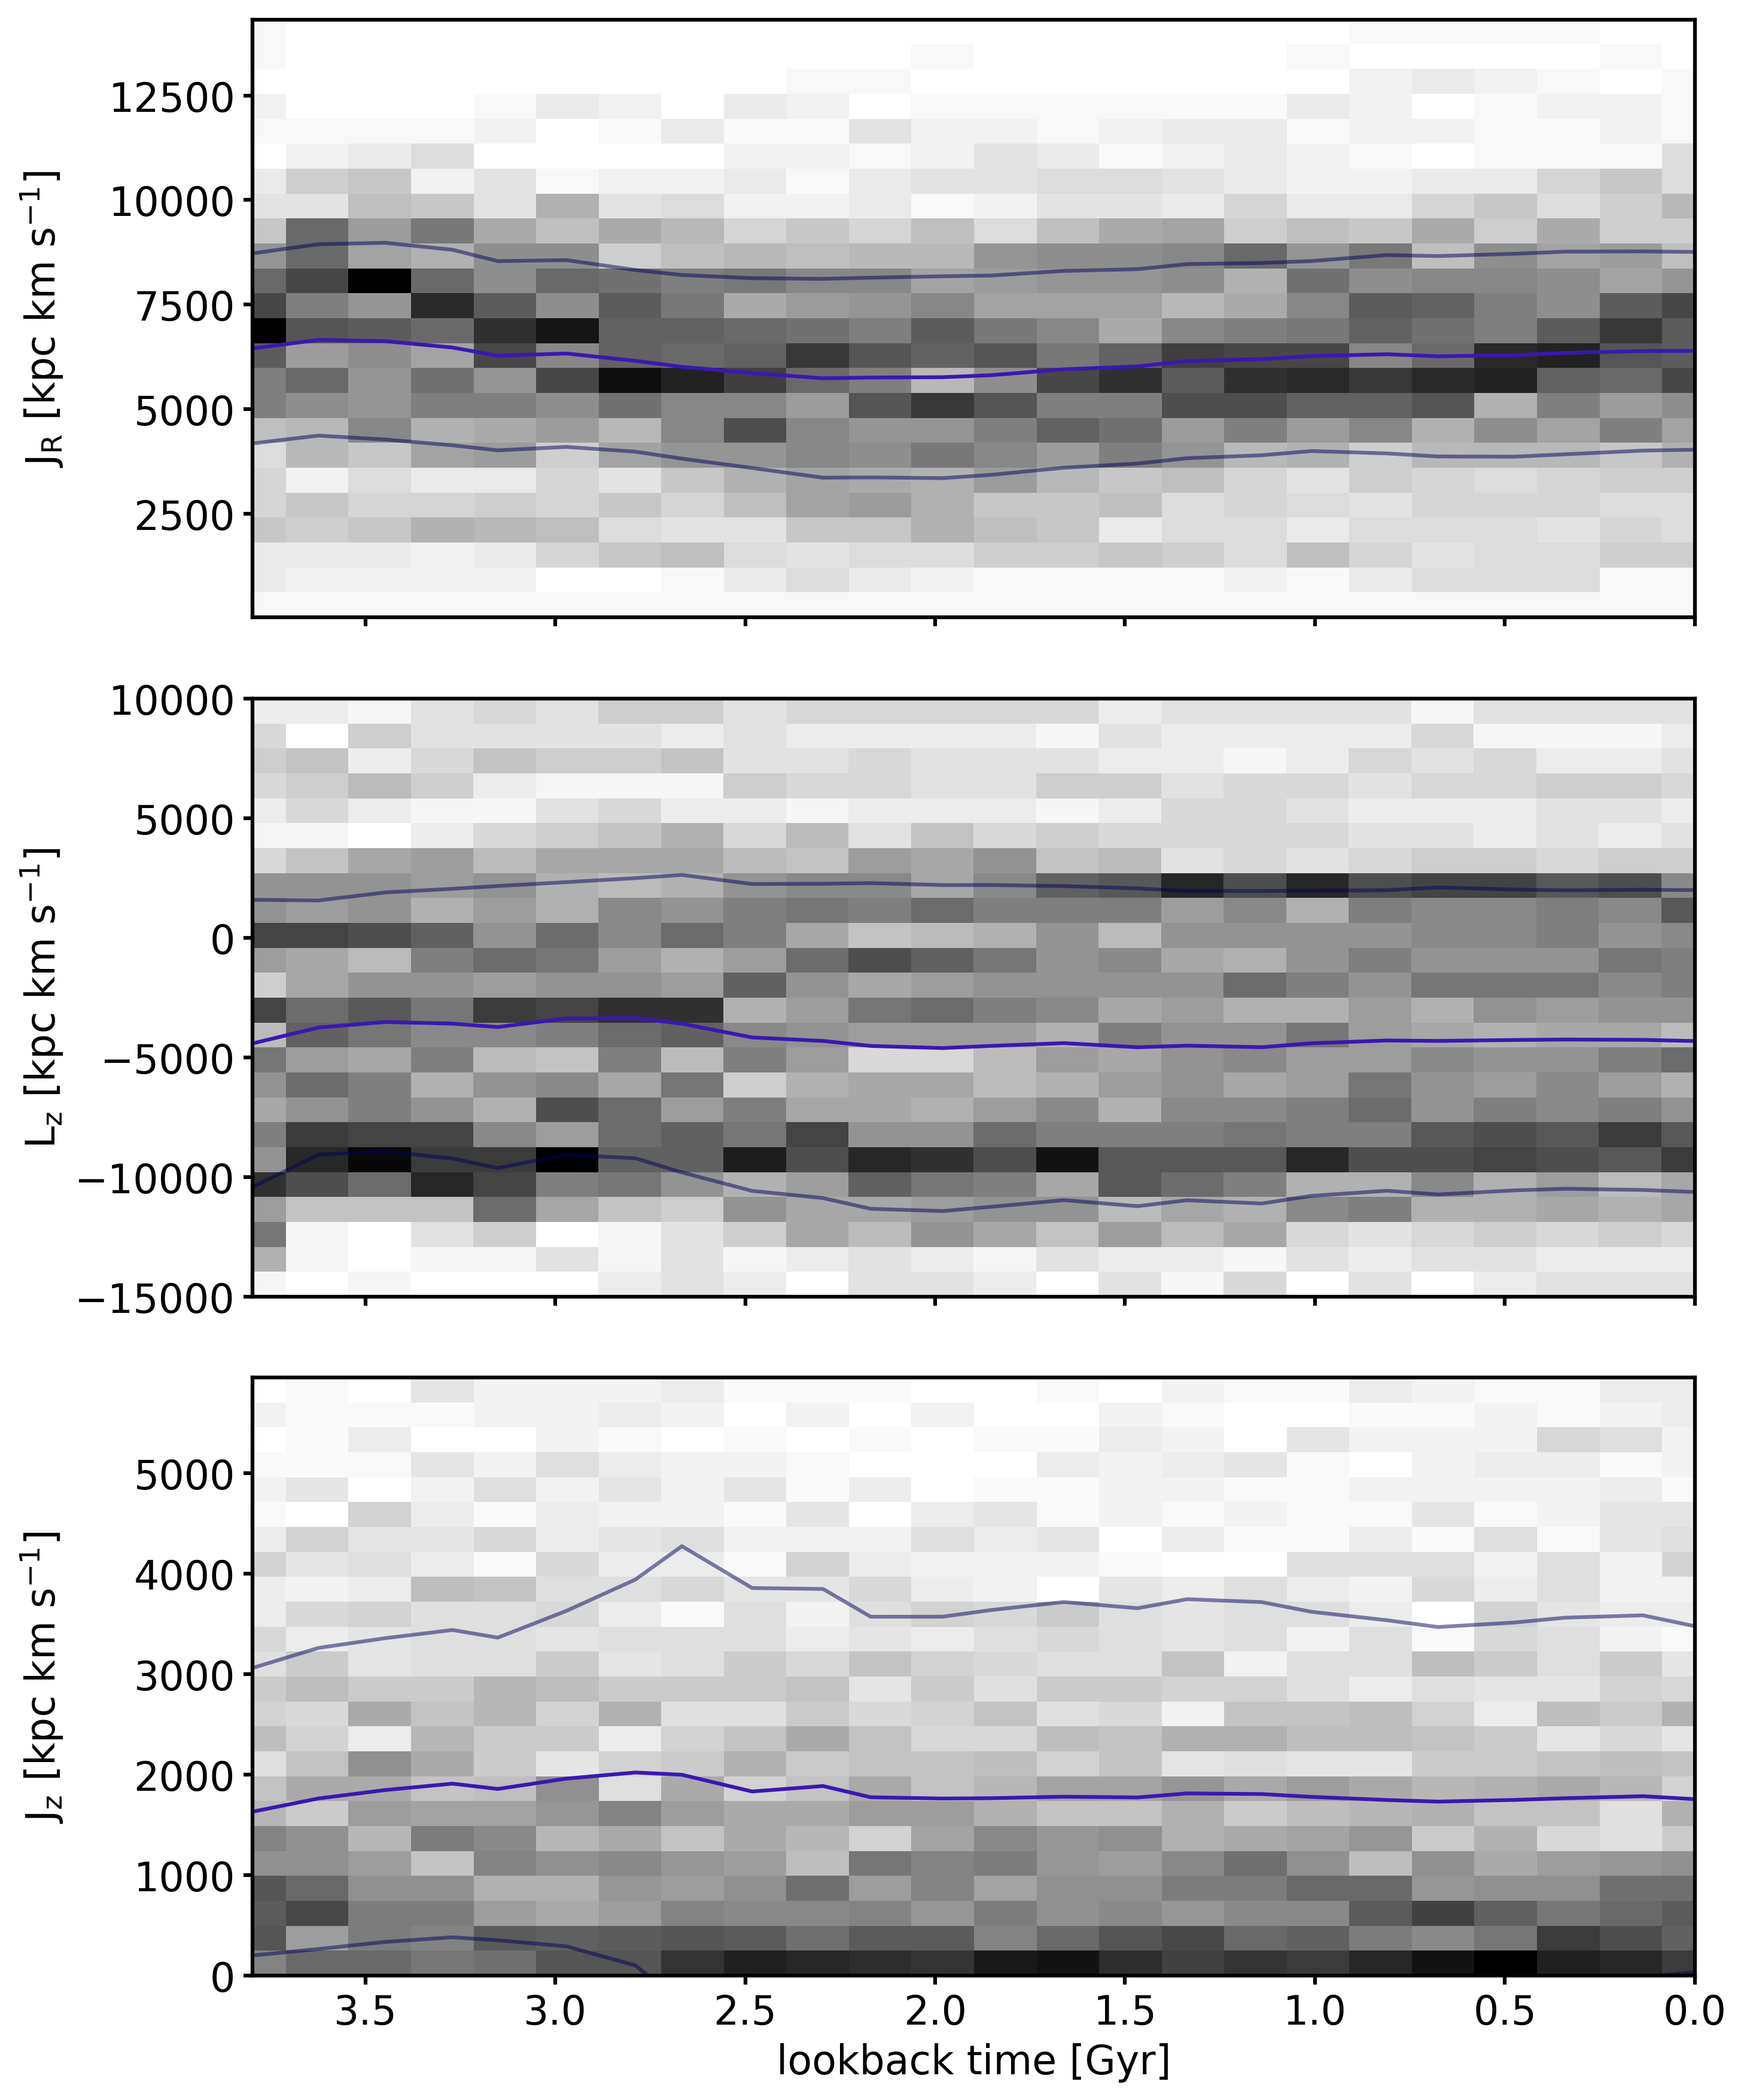
\includegraphics[width=\textwidth]{plots/Dynamics/mean_pot/action_time_evolution_hist_mean_prog3.png}
    \caption{Same as Figure \ref{fig:actions_time_evolution_prog3}, only for a constant potential since the merger of prog2.}\label{fig:actions_time_evolution_mean_pot_prog3}
\end{figure}

\begin{figure}[htbp]
\captionsetup{format=plain}
    \centering
	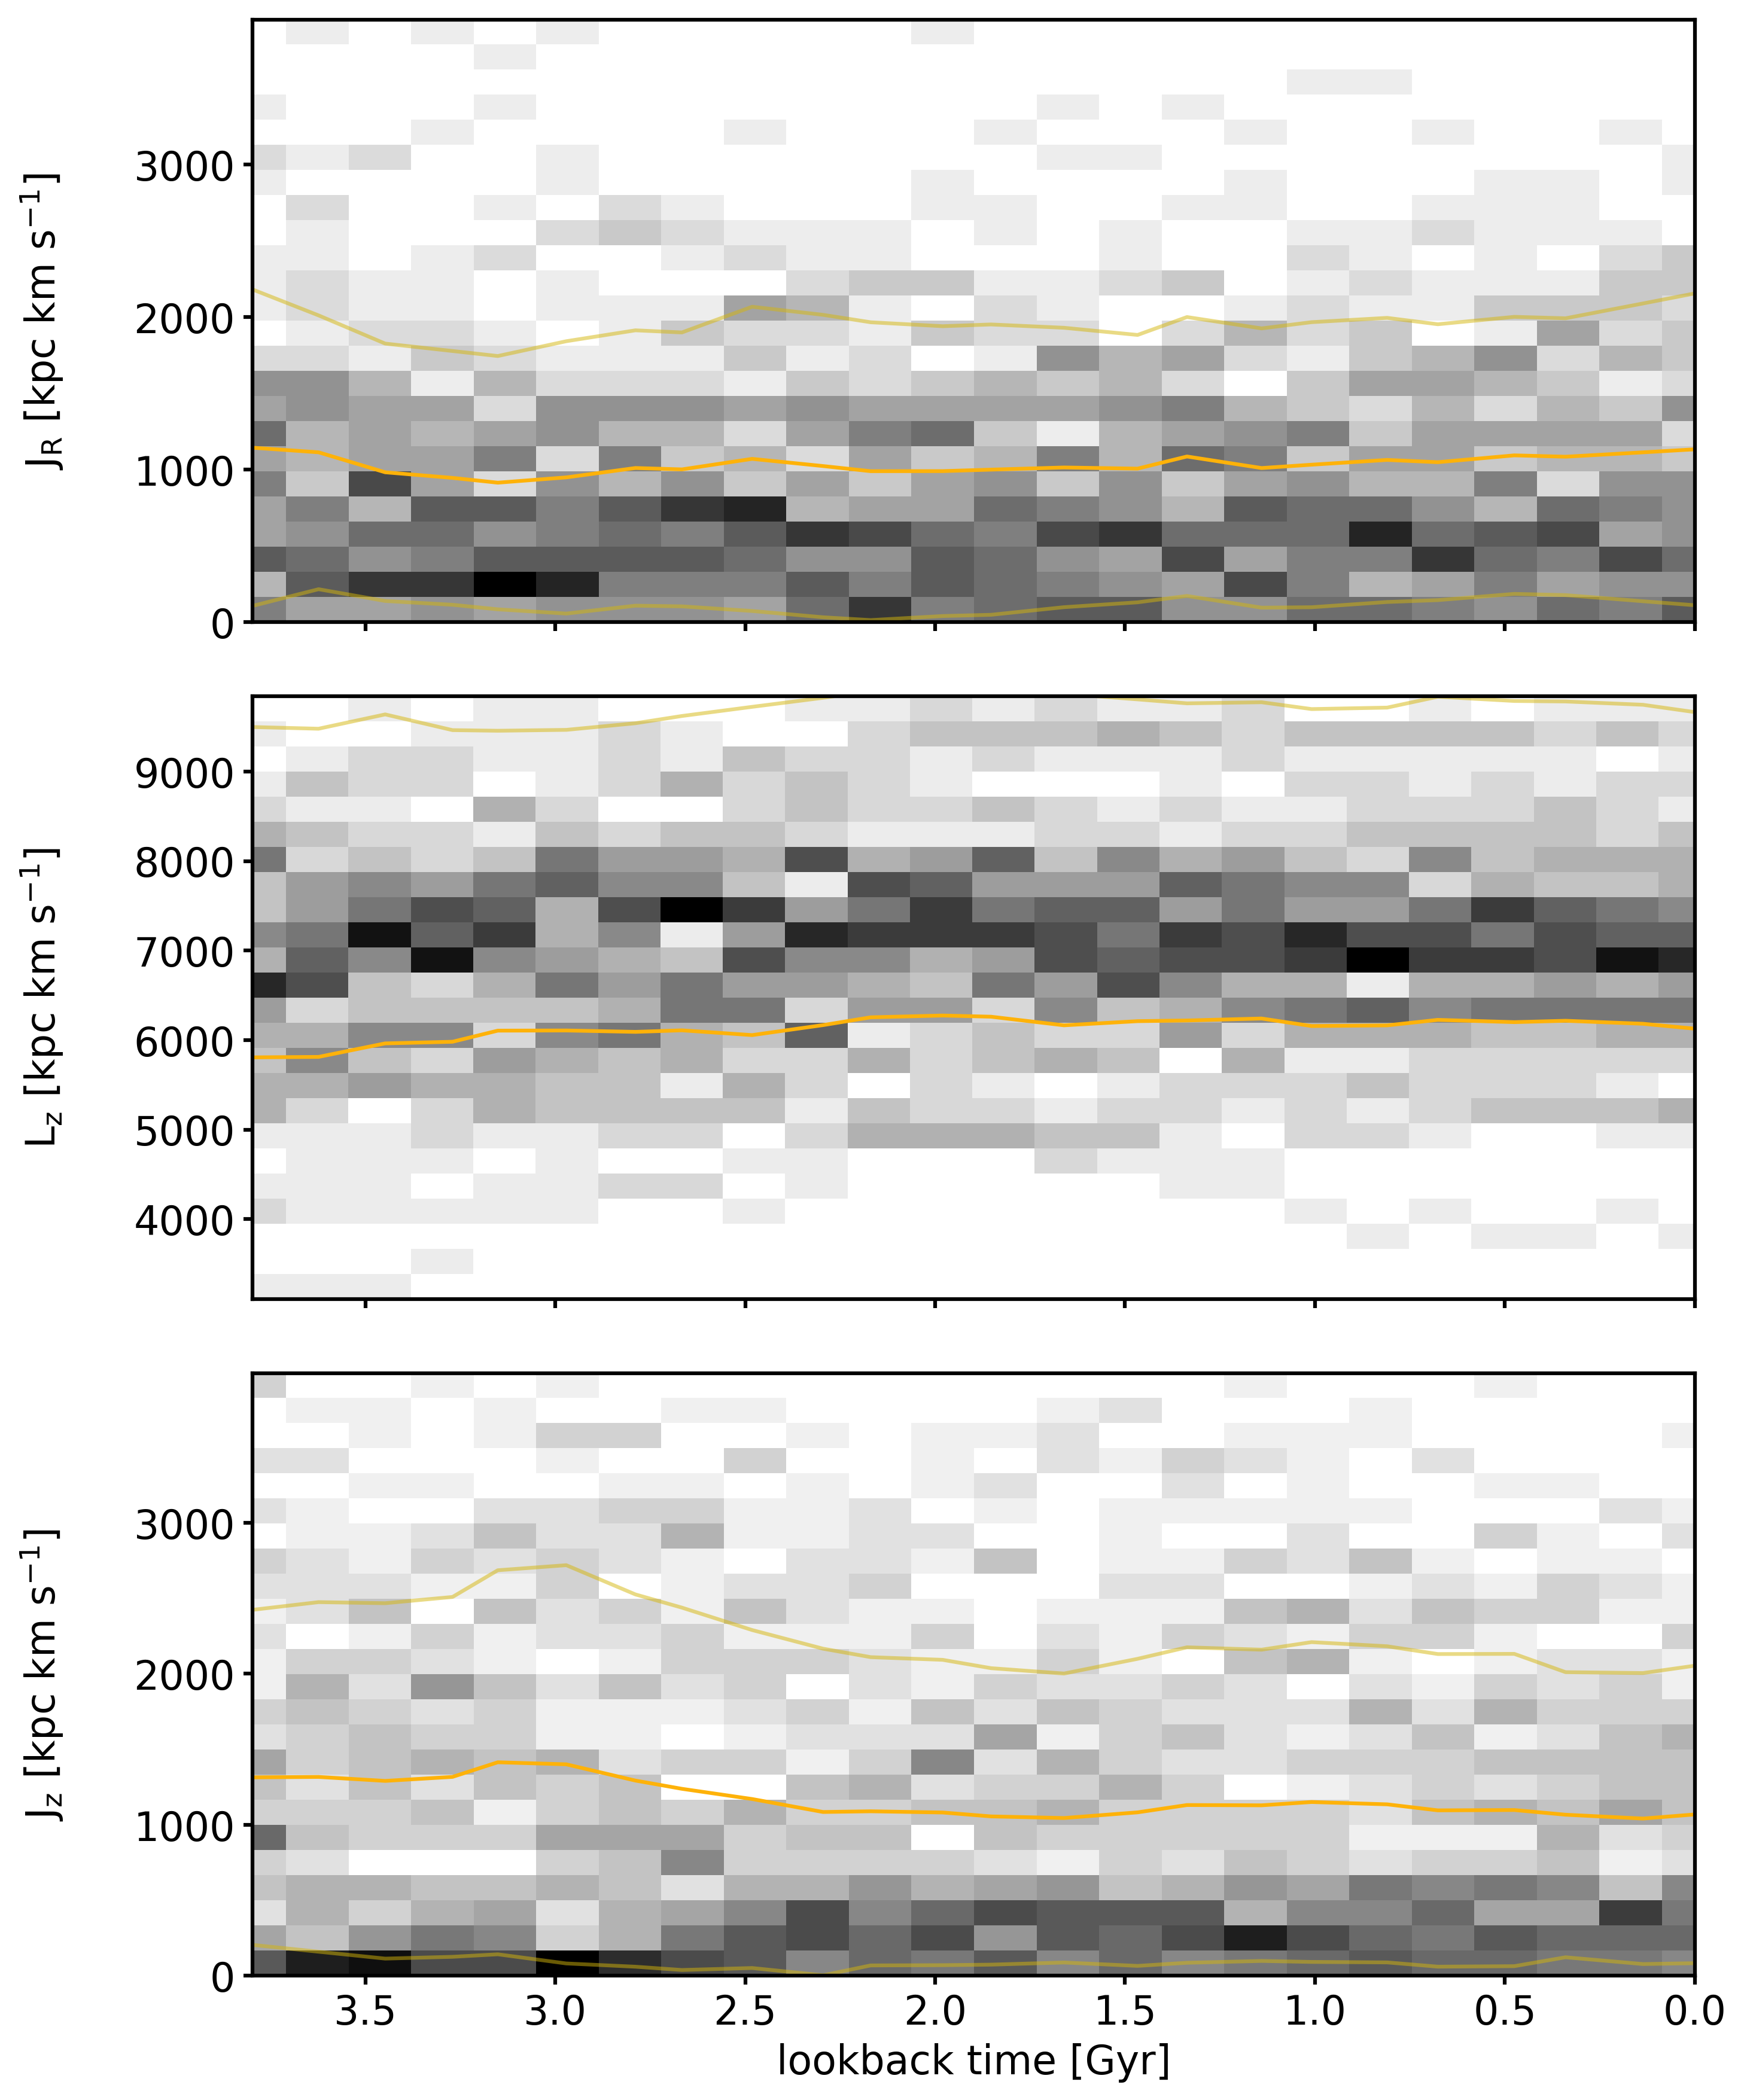
\includegraphics[width=\textwidth]{plots/Dynamics/mean_pot/action_time_evolution_hist_mean_prog4.png}
    \caption{Same as Figure \ref{fig:actions_time_evolution_prog4}, only for a constant potential since the merger of prog2.}\label{fig:actions_time_evolution_mean_pot_prog4}
\end{figure}
\fi

\subsubsection{Energy evolution}\label{subsubsec:energy_evol}
Another assumption under which we calculated the radial and vertical actions were the use of the action estimation method "St\"ackel Fudge". To test if variations and the missing of clumpiness could be due to estimation inaccuracies or numerical problems in this approach we can have a look at the other \ac{IoM}, angular momentum and energy. Since $L_z$ was rather constant in Figures \ref{fig:actions_time_evolution_prog2} - \ref{fig:actions_time_evolution_prog4} and \ref{fig:comparison_actions_time_evolution_mean_pot_prog2} we now evaluate the energy. It is calculated according to Equation \ref{eq:energy_hamiltonian} where $v^2 = \Sigma\limits_{i=1}^3 v_i^2$. We can derive the energy directly from the data by taking the potential value from the simulation. We also compare it to our potential model. The kinematic term of Equation \ref{eq:energy_hamiltonian} is identical for data and model.

\begin{figure}[htbp]
\captionsetup{format=plain}
    \centering
	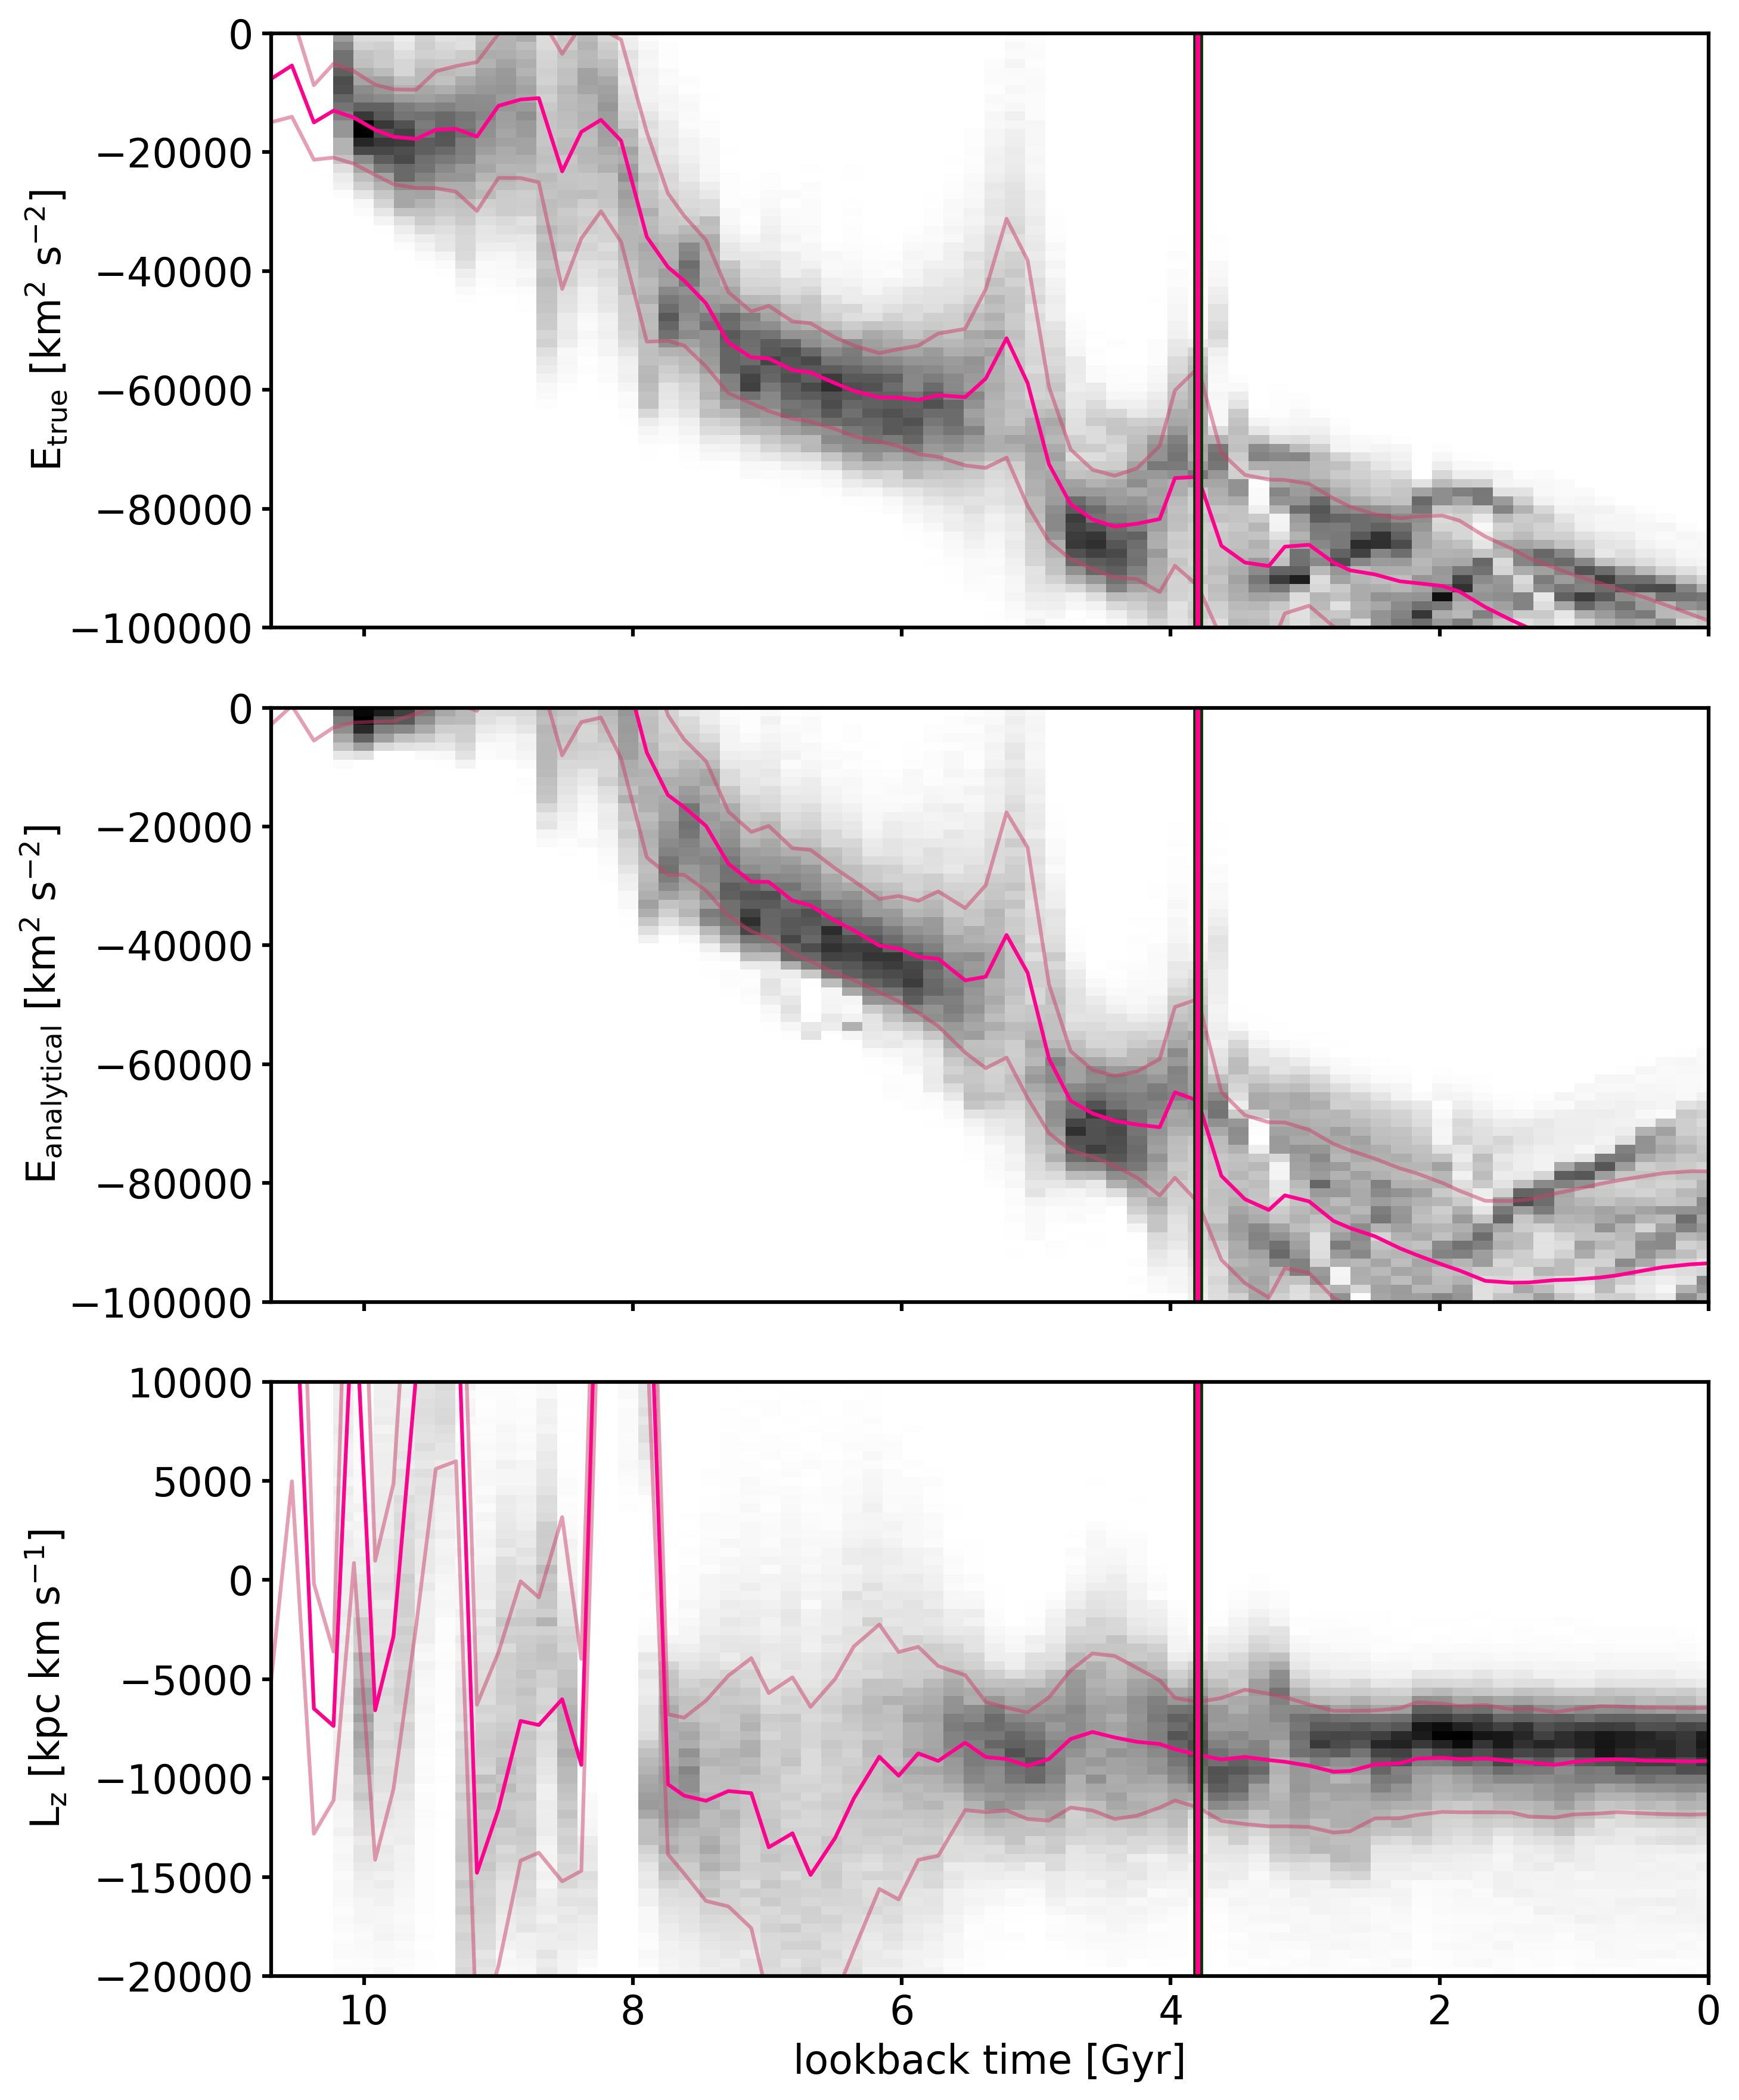
\includegraphics[width=\textwidth]{plots/Dynamics/prog2/energy_time_evolution_hist_mean.png}
	\caption{Time evolution of the energy of the particles of prog2. \textit{Upper panel}: The true energy, which the particles have according to their kinetic energy and their potential value as returned by the Auriga simulation. \textit{Middle panel}: Energy calculated in the interpolated best fit potential. \textit{Lower panel}: Angular momentum.\textcolor{red}{update with new selected GCs coming}}\label{fig:energy_time_evolution_prog2}
\end{figure}

We show the energy evolution in Figure \ref{fig:energy_time_evolution_prog2}. Here it again becomes obvious, that the potential fit could be better since the model overestimates the energy by a few \SI{1000}{km^{2}.s^{-2}}. It is in agreement with the absolute error of the potential (see Figure \ref{fig:potential_fit_abs_errors}) which translates to only a small relative error (Figure \ref{fig:potential_best_fit} lower panel). The overall trend is still similar. As the \ac{DG} spirals in it falls deeper into the potential well. This trend continues even after the merger. Therefore it still loses energy. We find the same trend for prog3 and prog4. We observe small scale variations in the energy, similarly to what is seen in the actions (best seen in $J_R$ in Figure \ref{fig:actions_time_evolution_prog3}.
\\\\\textcolor{red}{check language}This gives another evidence that within our goal to evaluate the galaxy in an analytic axisymmetric form we do not have problems with our assumptions but it seems that the simulation is just too complex to model it that simply.

\iffalse
\begin{figure}
\captionsetup{format=plain}
    \centering
	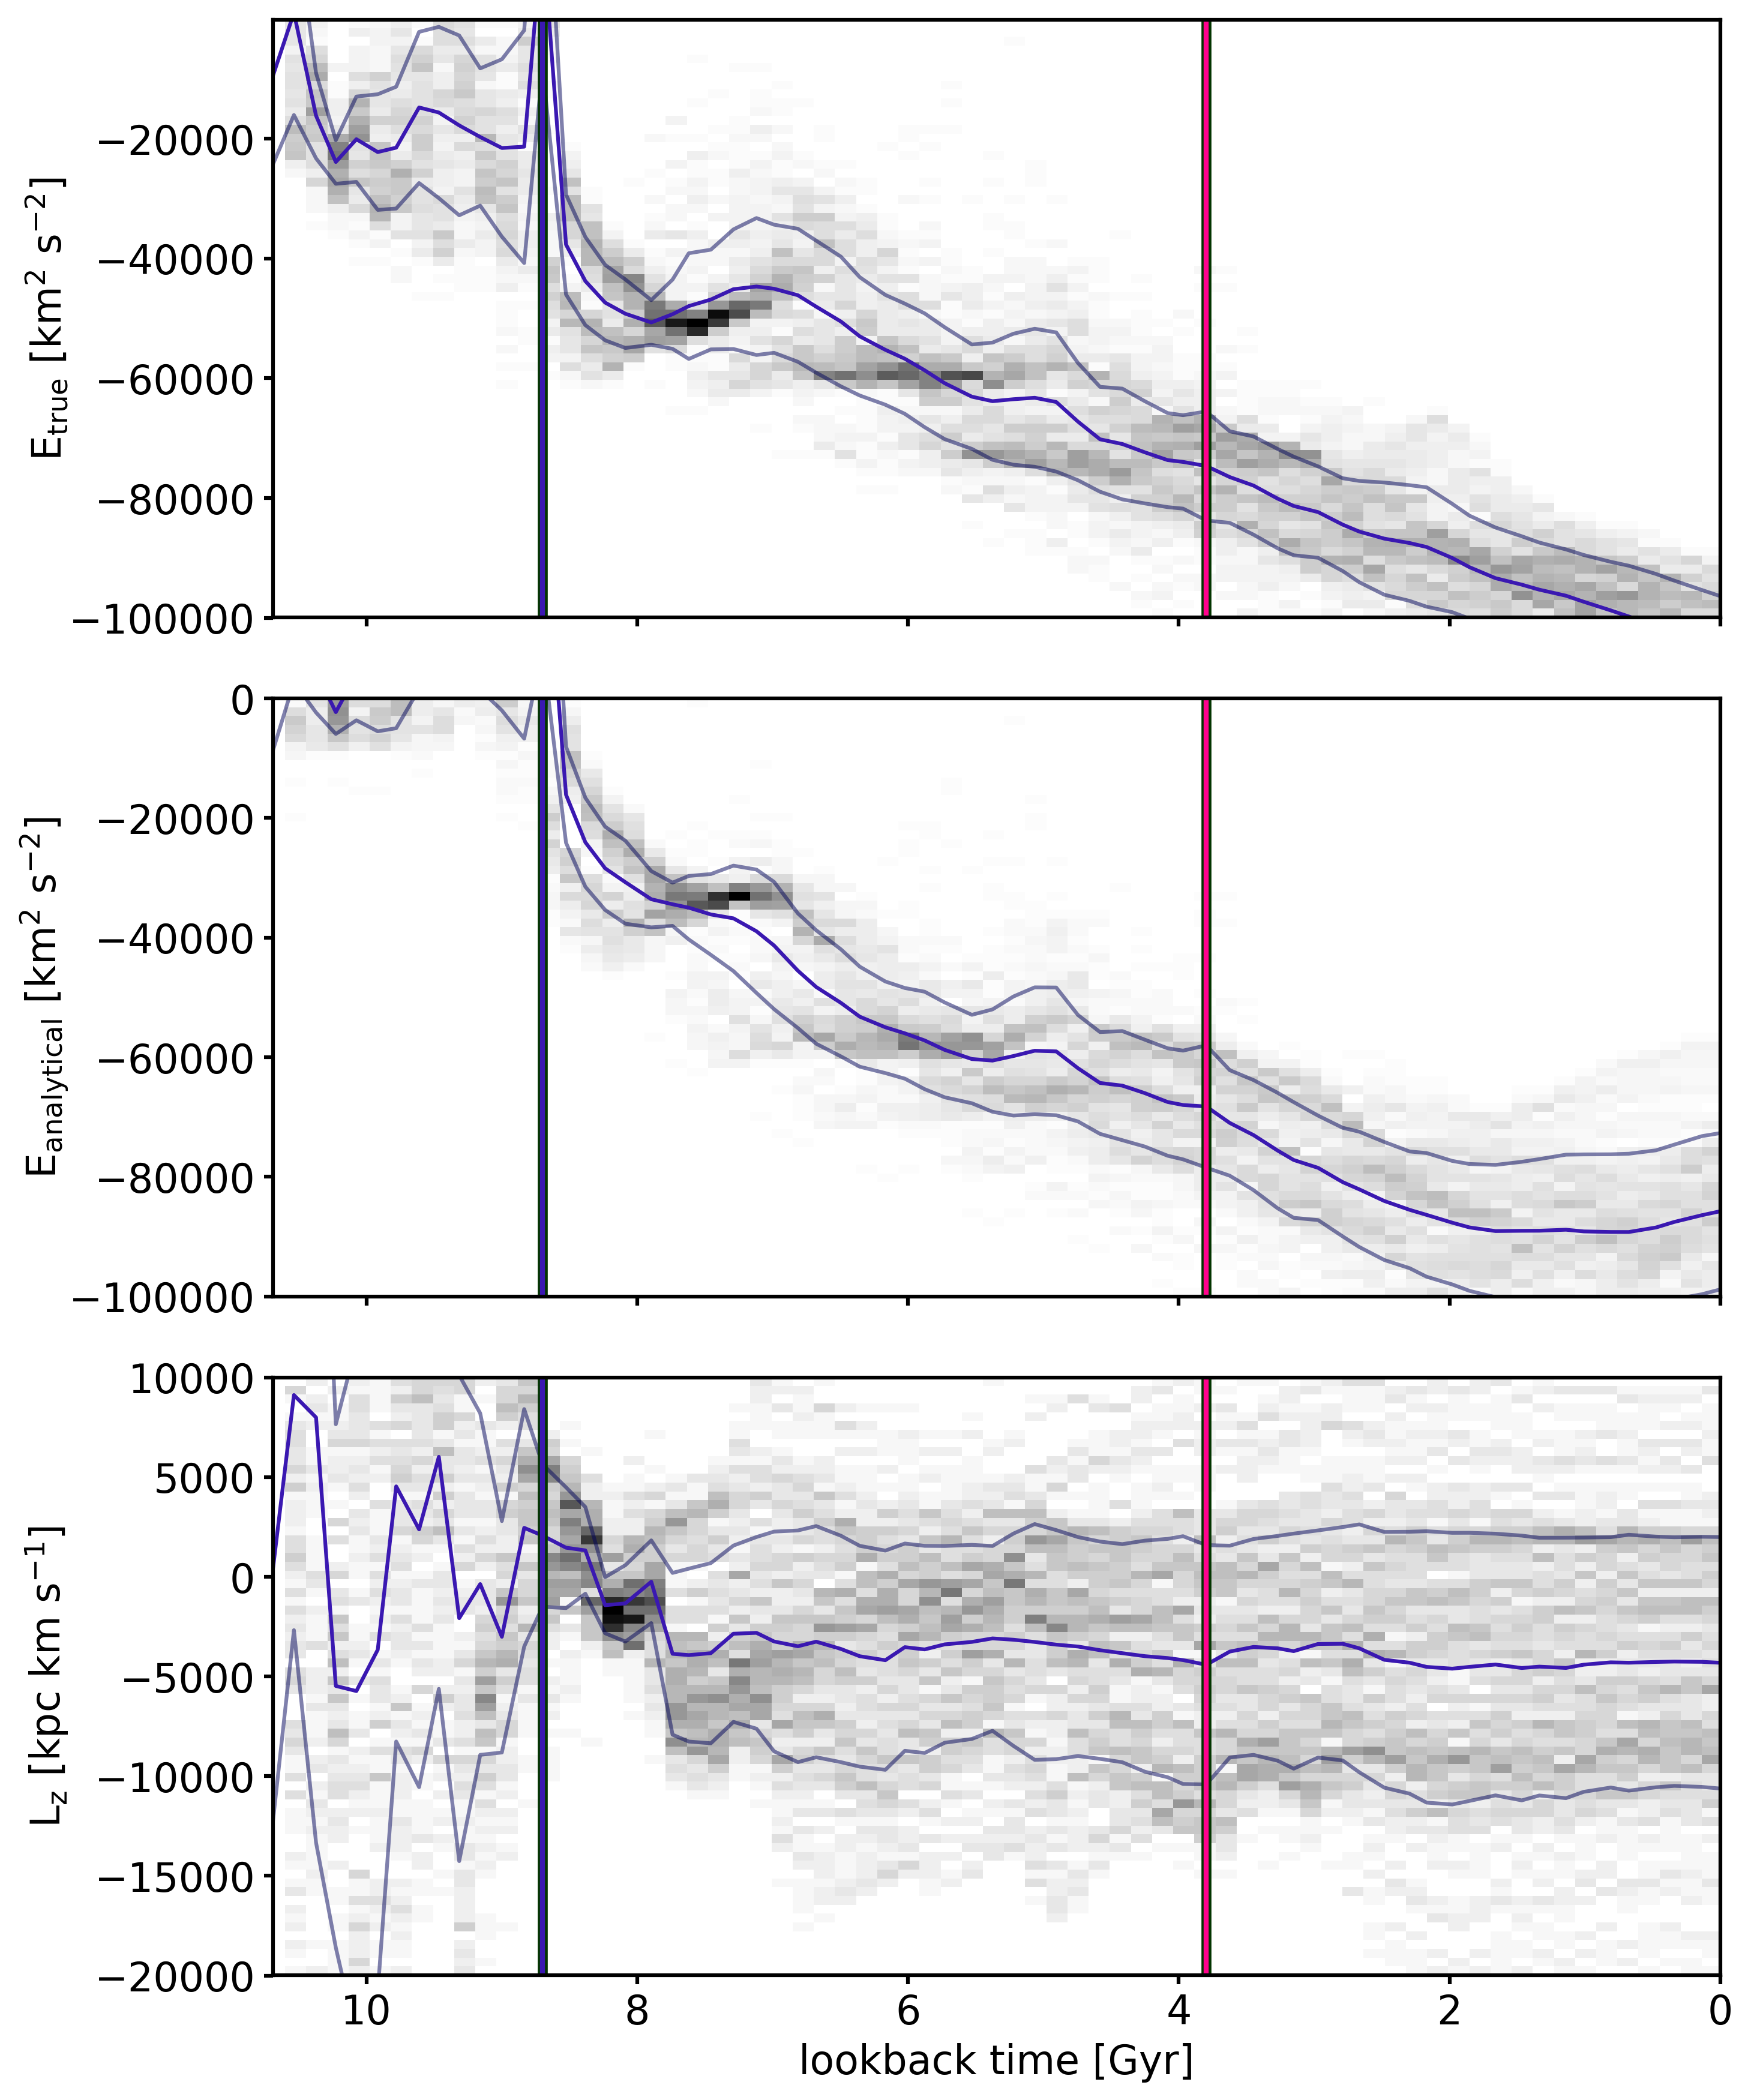
\includegraphics[width=\textwidth]{plots/Dynamics/prog3/energy_time_evolution_hist_mean.png}
    \caption{Same as \ref{fig:energy_time_evolution_prog2} but for prog3. }\label{fig:energy_time_evolution_prog3}
\end{figure}

\begin{figure}[htbp]
\captionsetup{format=plain}
    \centering
	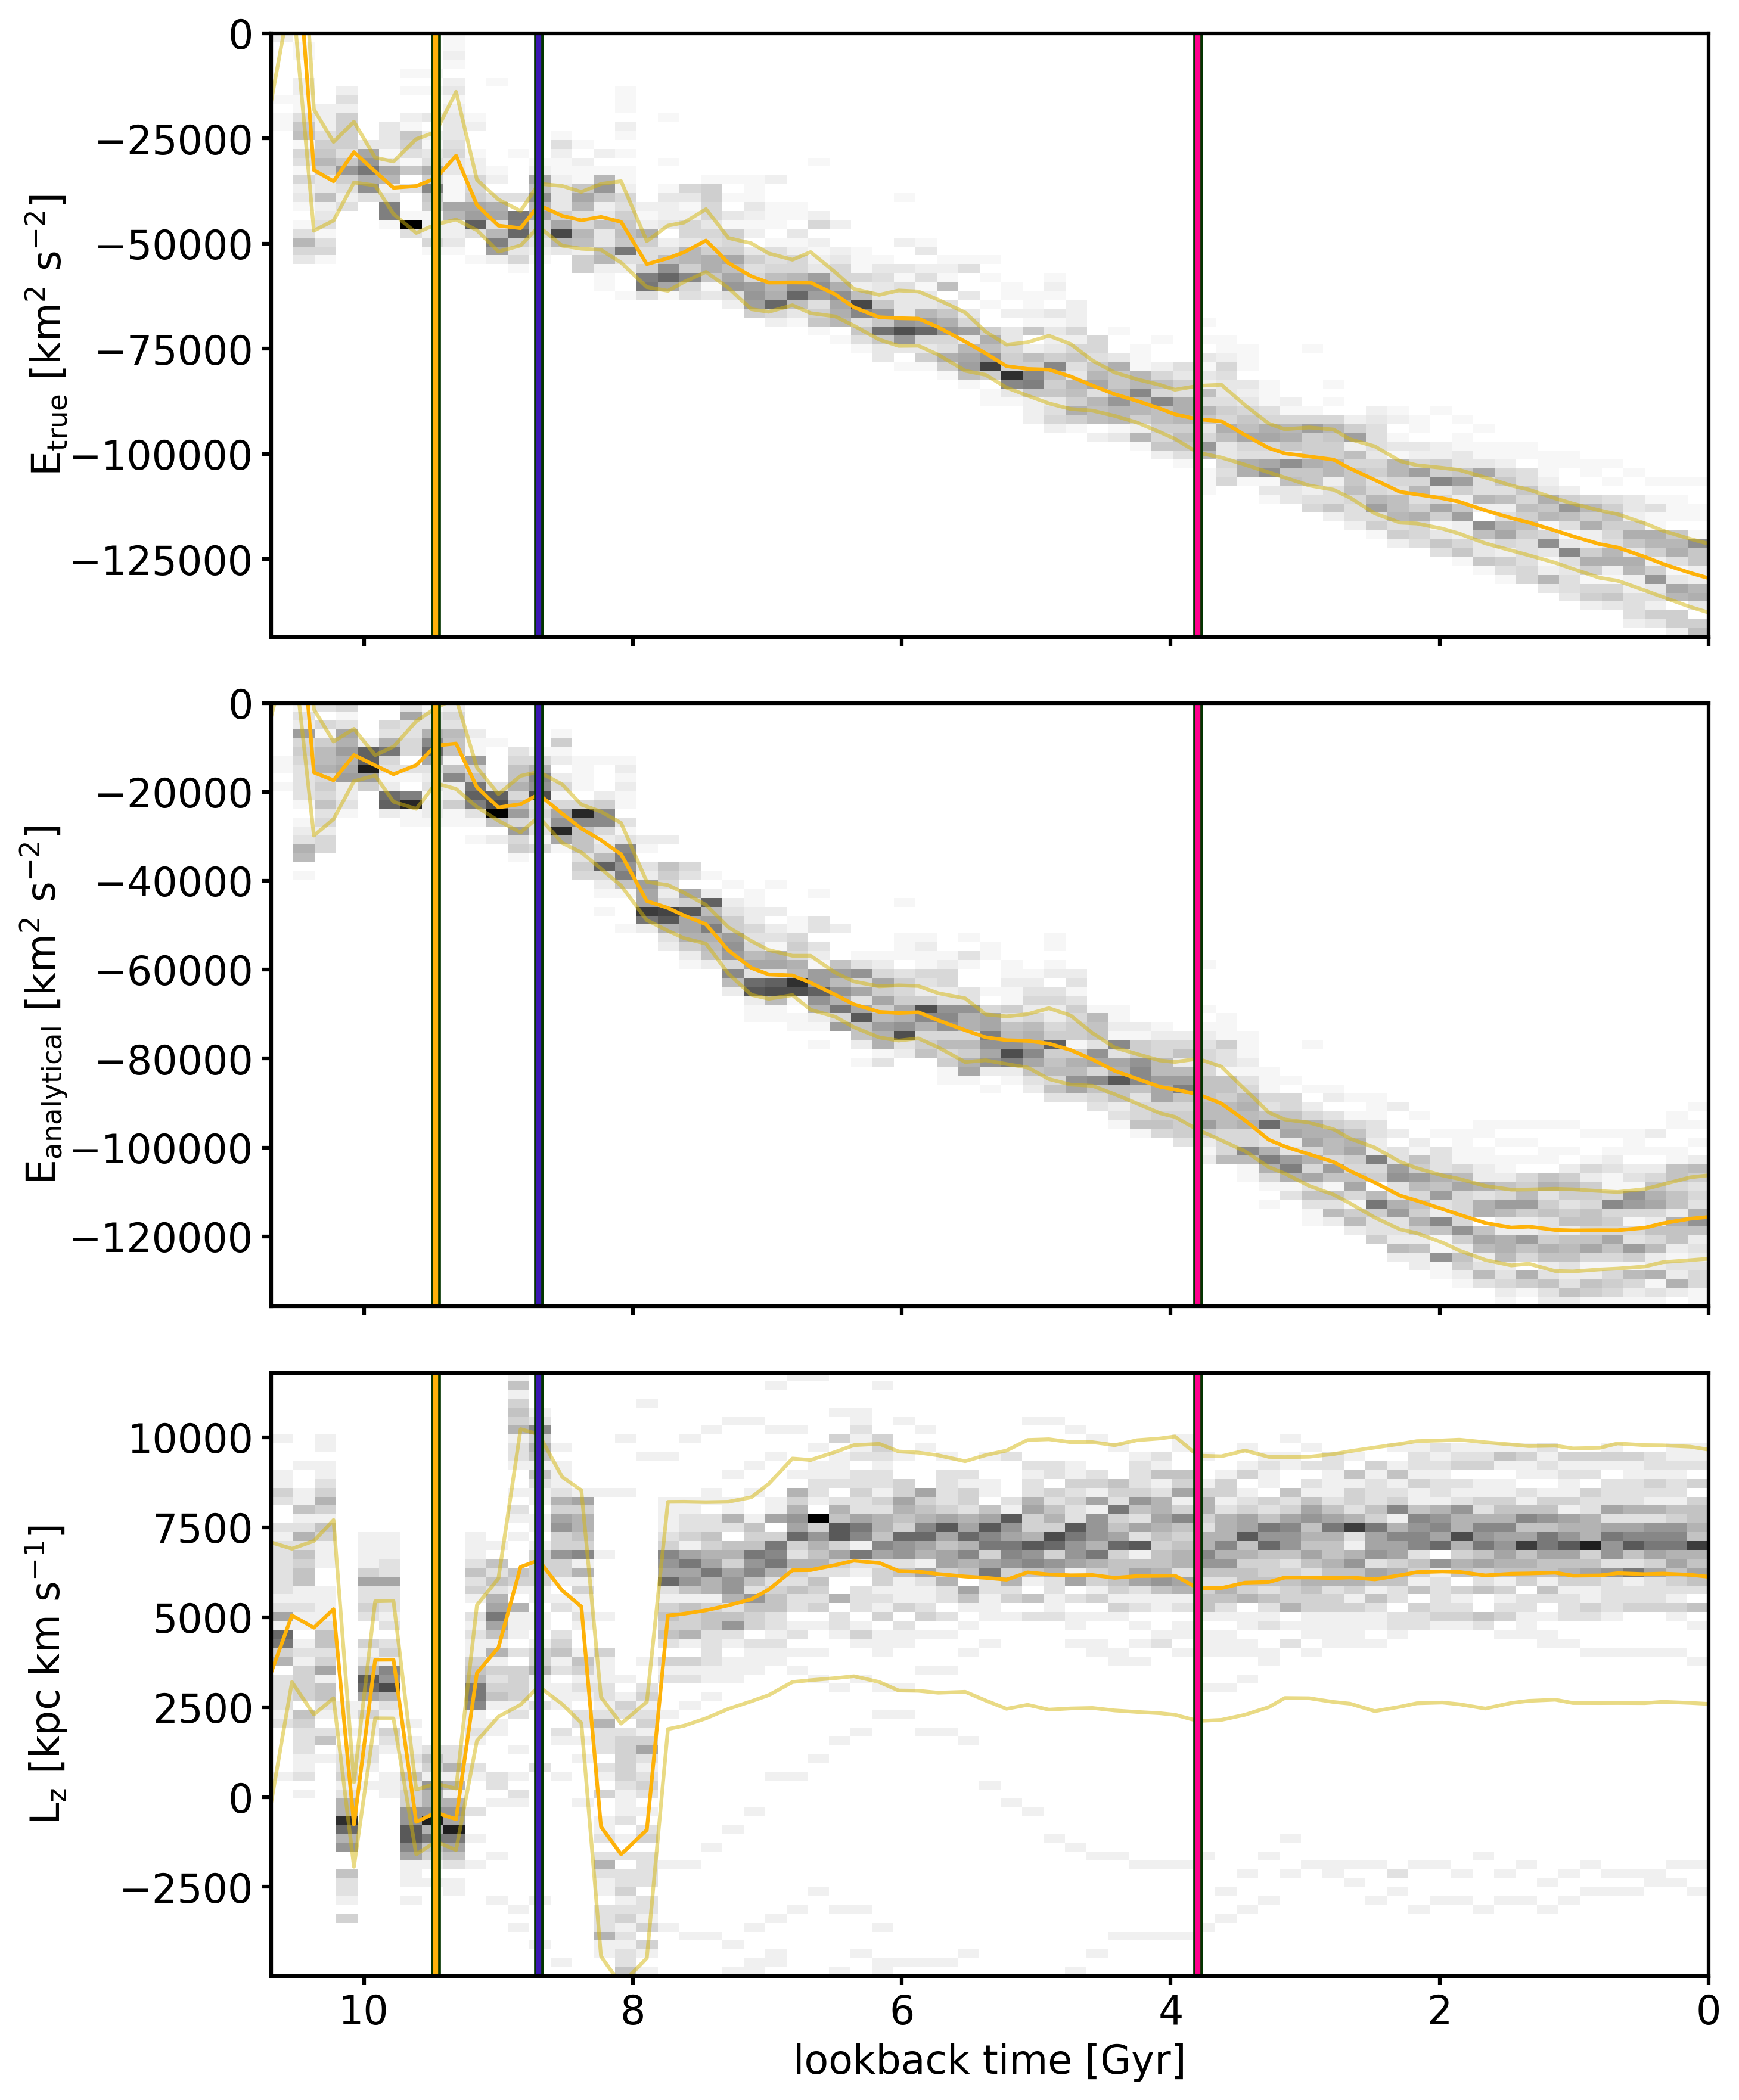
\includegraphics[width=\textwidth]{plots/Dynamics/prog4/energy_time_evolution_hist_mean.png}
    \caption{ame as \ref{fig:energy_time_evolution_prog2} but for prog4.}\label{fig:energy_time_evolution_prog4}
\end{figure}
\fi

\subsection{Test: evolution of globular clusters on same orbit at $z=0$}\label{subsec:box_GCs}
In Section \ref{subsec:GCs_action_space} we found that the overall \ac{GC} distribution in action space is not very clumped. In Section \ref{subsec:time_evo_actions} we saw a rather constant evolution of the actions but with a large scatter. Now we investigate \acp{GC} whose actions are close together in the last snapshot. The selection of these "box \acp{GC}" is made by taking the mean of each action and find all \acp{GC} within a cube centered on the means with a gradually increasing side length. For prog2, we want to look at a larger of 20 particles. To have 20 particles in this cube required a side length of \SI{650}{kpc.km.s^{-1}}. Since we have fewer particles accreted from prog3 and prog4, they needed bigger side lengths and therefore the orbits of their box particles are a priori not as close.  

\begin{figure}[htbp]
\captionsetup{format=plain}
    \centering
    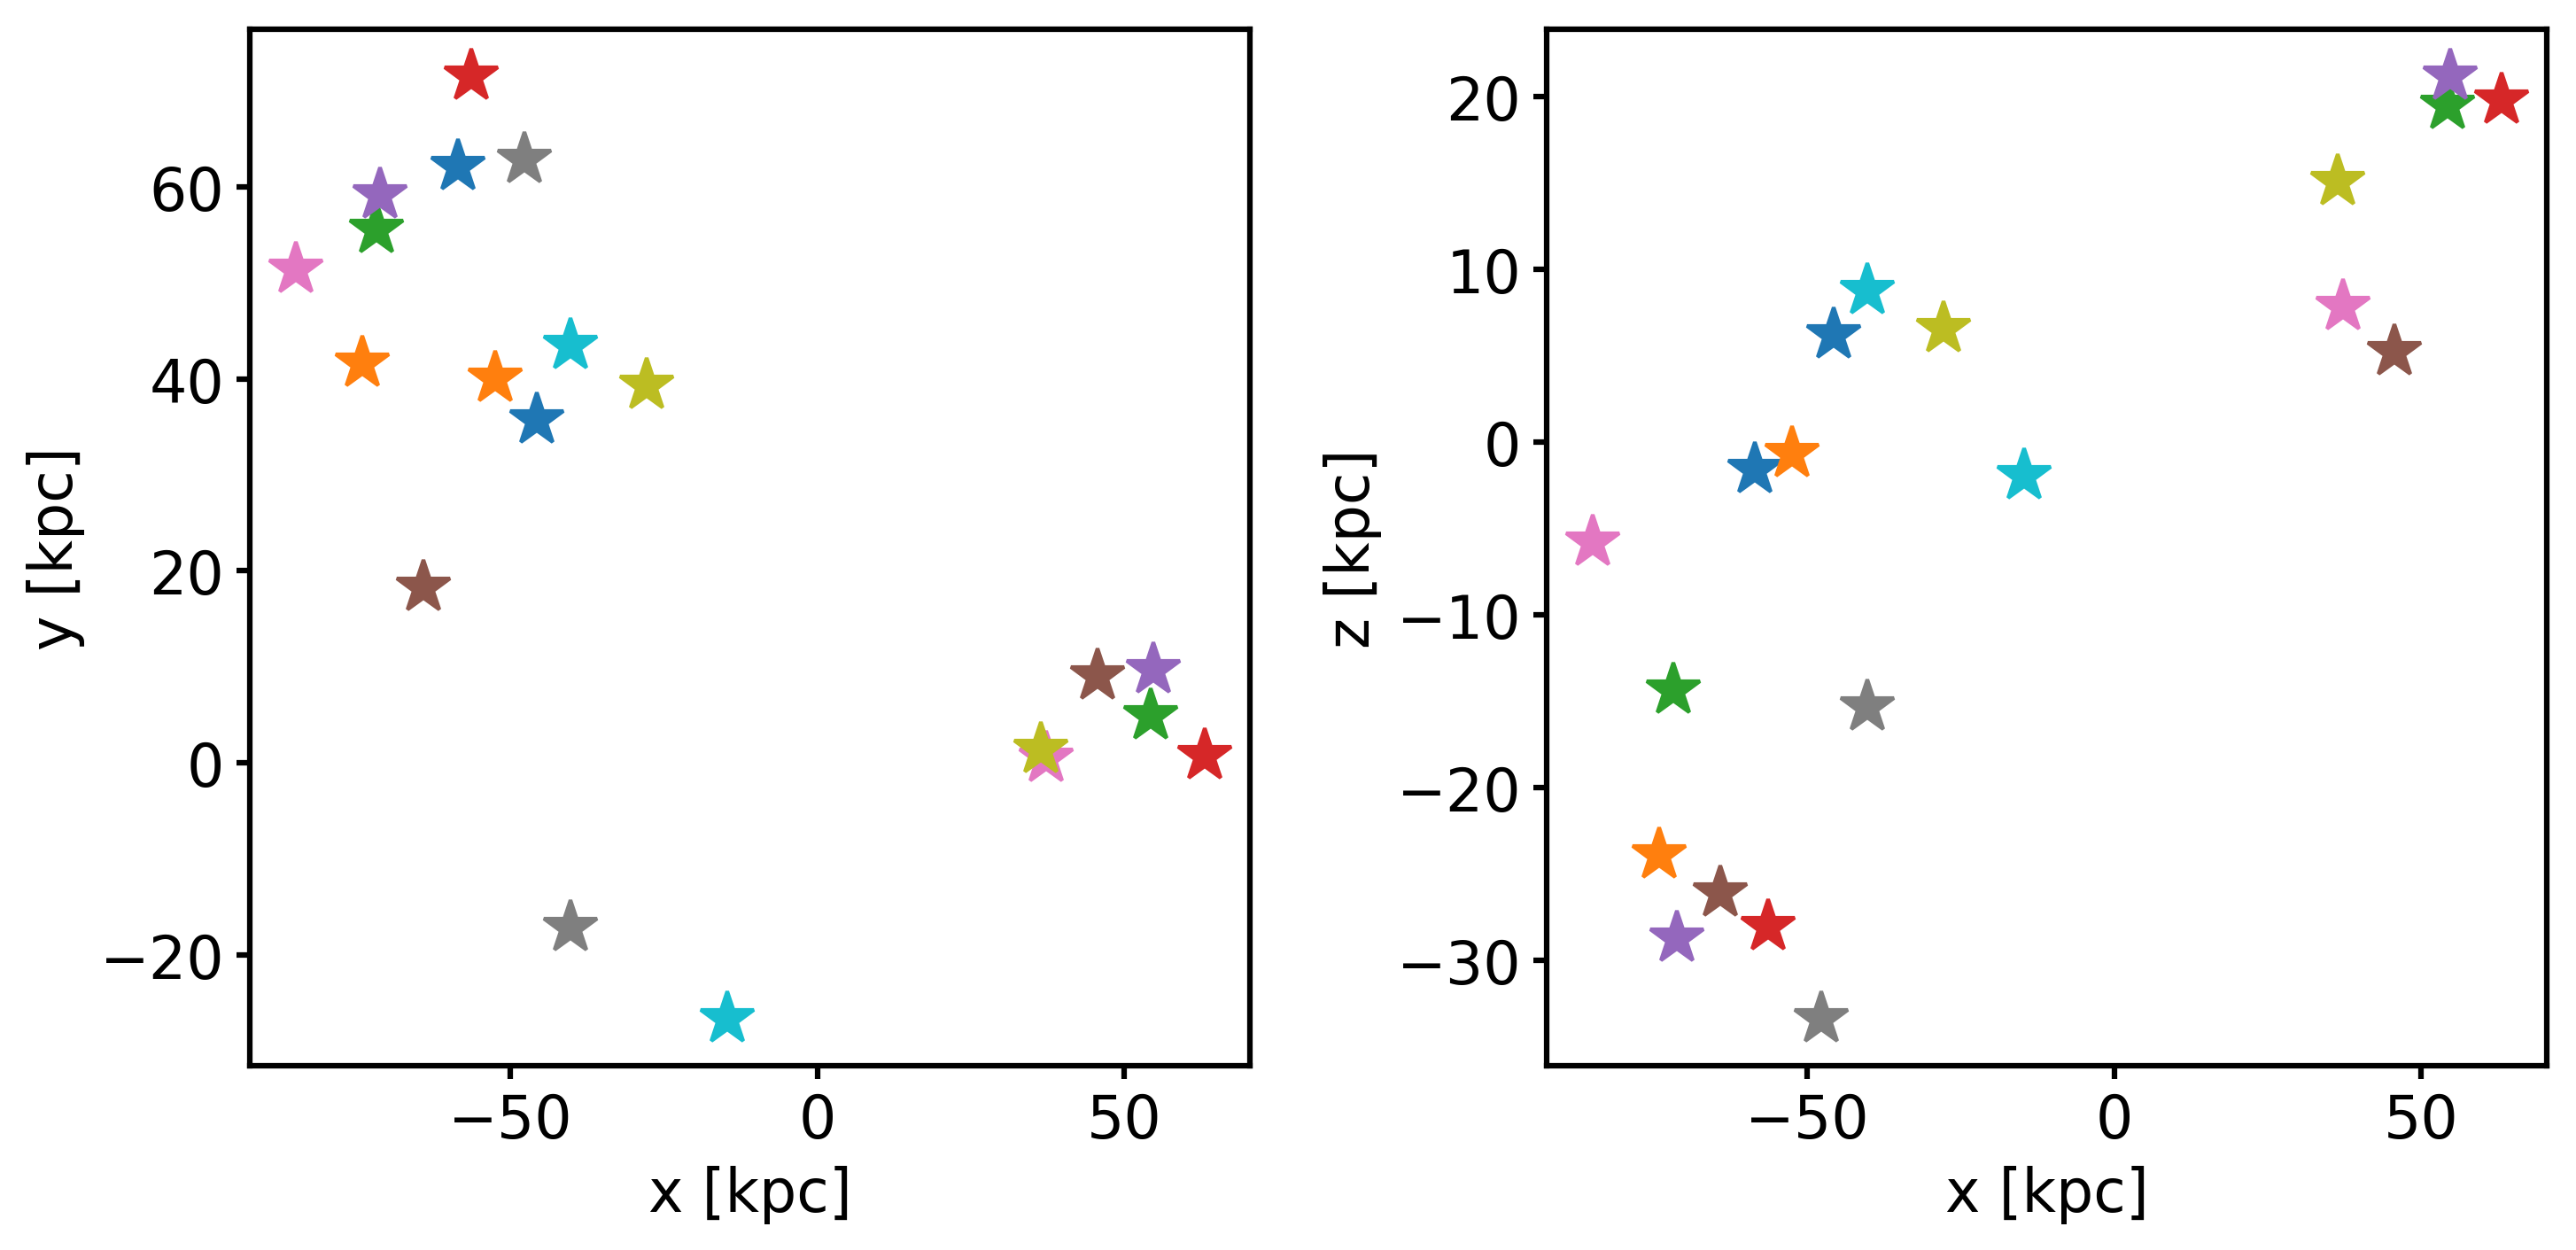
\includegraphics[width=0.9\textwidth]{plots/Dynamics/dist/progenitor2_box_distribution.png}
    \caption{Spatial distribution of selected box particles. \textcolor{red}{update with new selected GCs and therefore new boxcoming}}
    \label{fig:box_GCs_distr}
\end{figure}

Their spatial distribution is presented in Figure \ref{fig:box_GCs_distr}. There is a small clustering around $x = \SI{50}{kpc}$ but all other selected GCs are well distributed in space. 

\iffalse
\begin{figure}[htbp]
\captionsetup{format=plain}
    \centering
	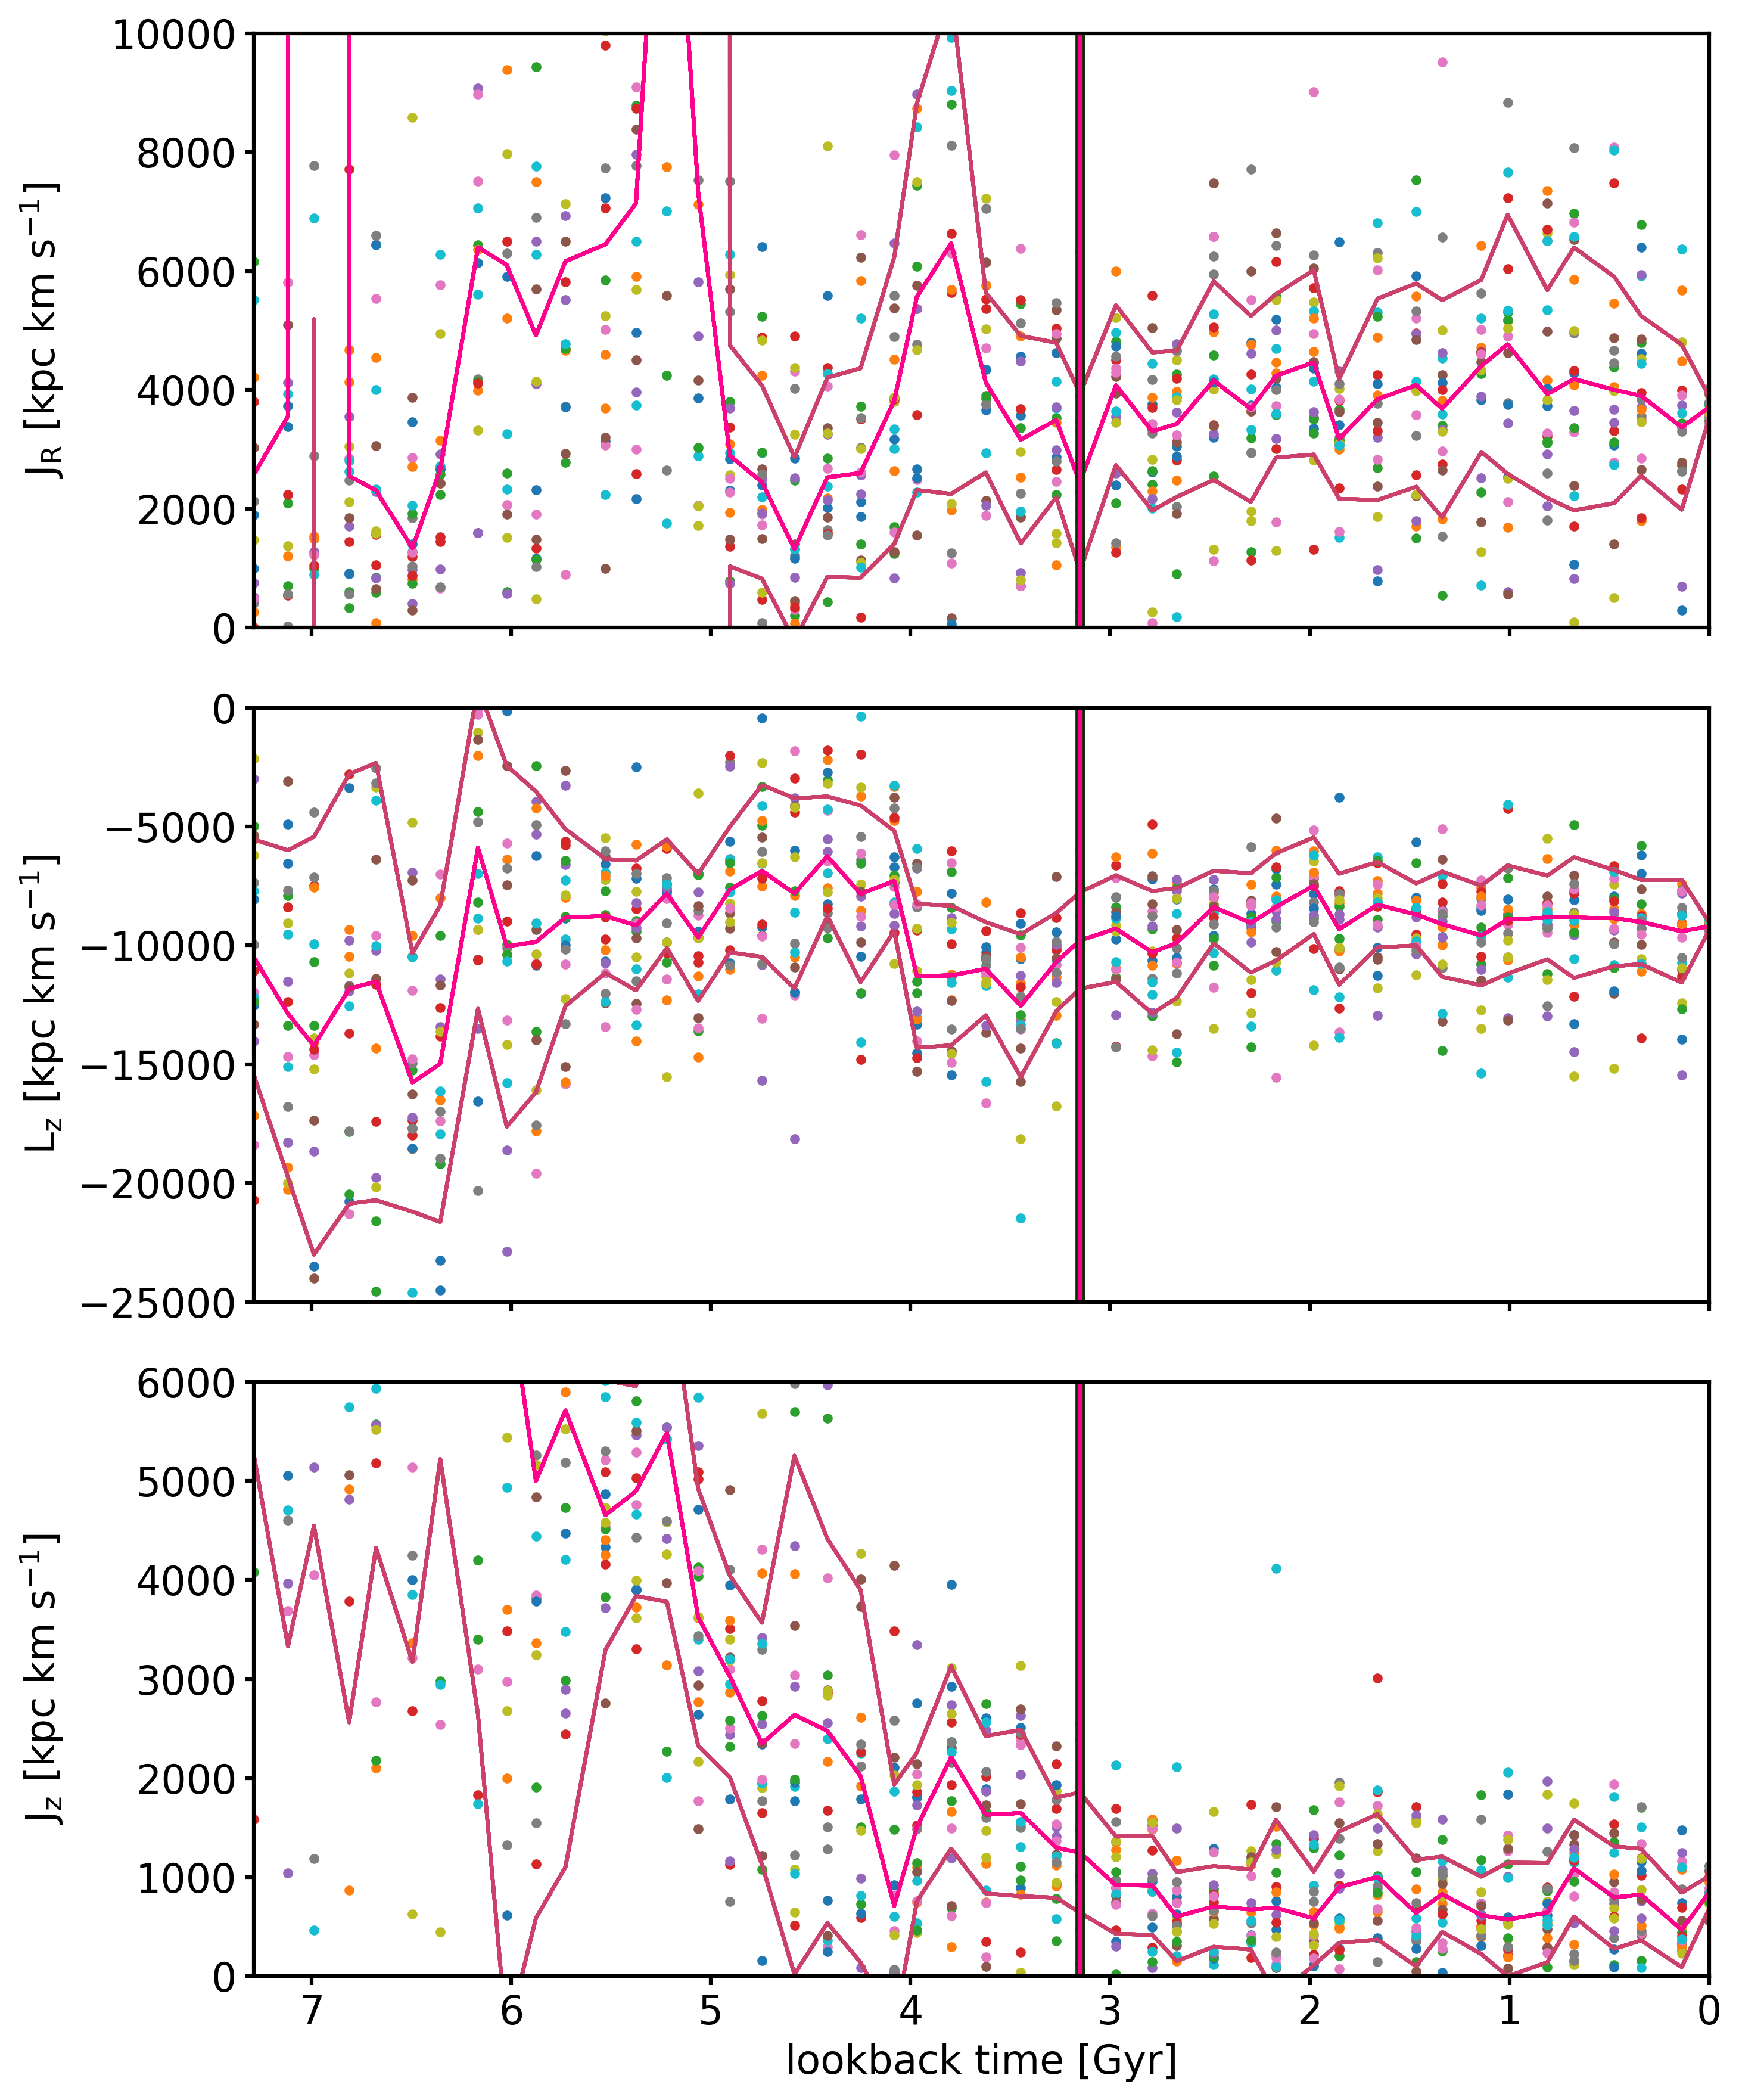
\includegraphics[width=\textwidth]{plots/Dynamics/prog2/action_time_evolution_box_hist_mean_prog2.png}

	\caption{Action time evolution of 17 particles of prog2 which are found to be on similar orbits in the $z=0$ snapshot. \textcolor{red}{update with new selected GCs and therefore new boxcoming} }\label{fig:actions_box_time_evolution_prog2}
\end{figure}
\fi


\begin{figure}[htbp]
\captionsetup{format=plain}
    \begin{subfigure}[c]{0.48\textwidth}
    \centering
    	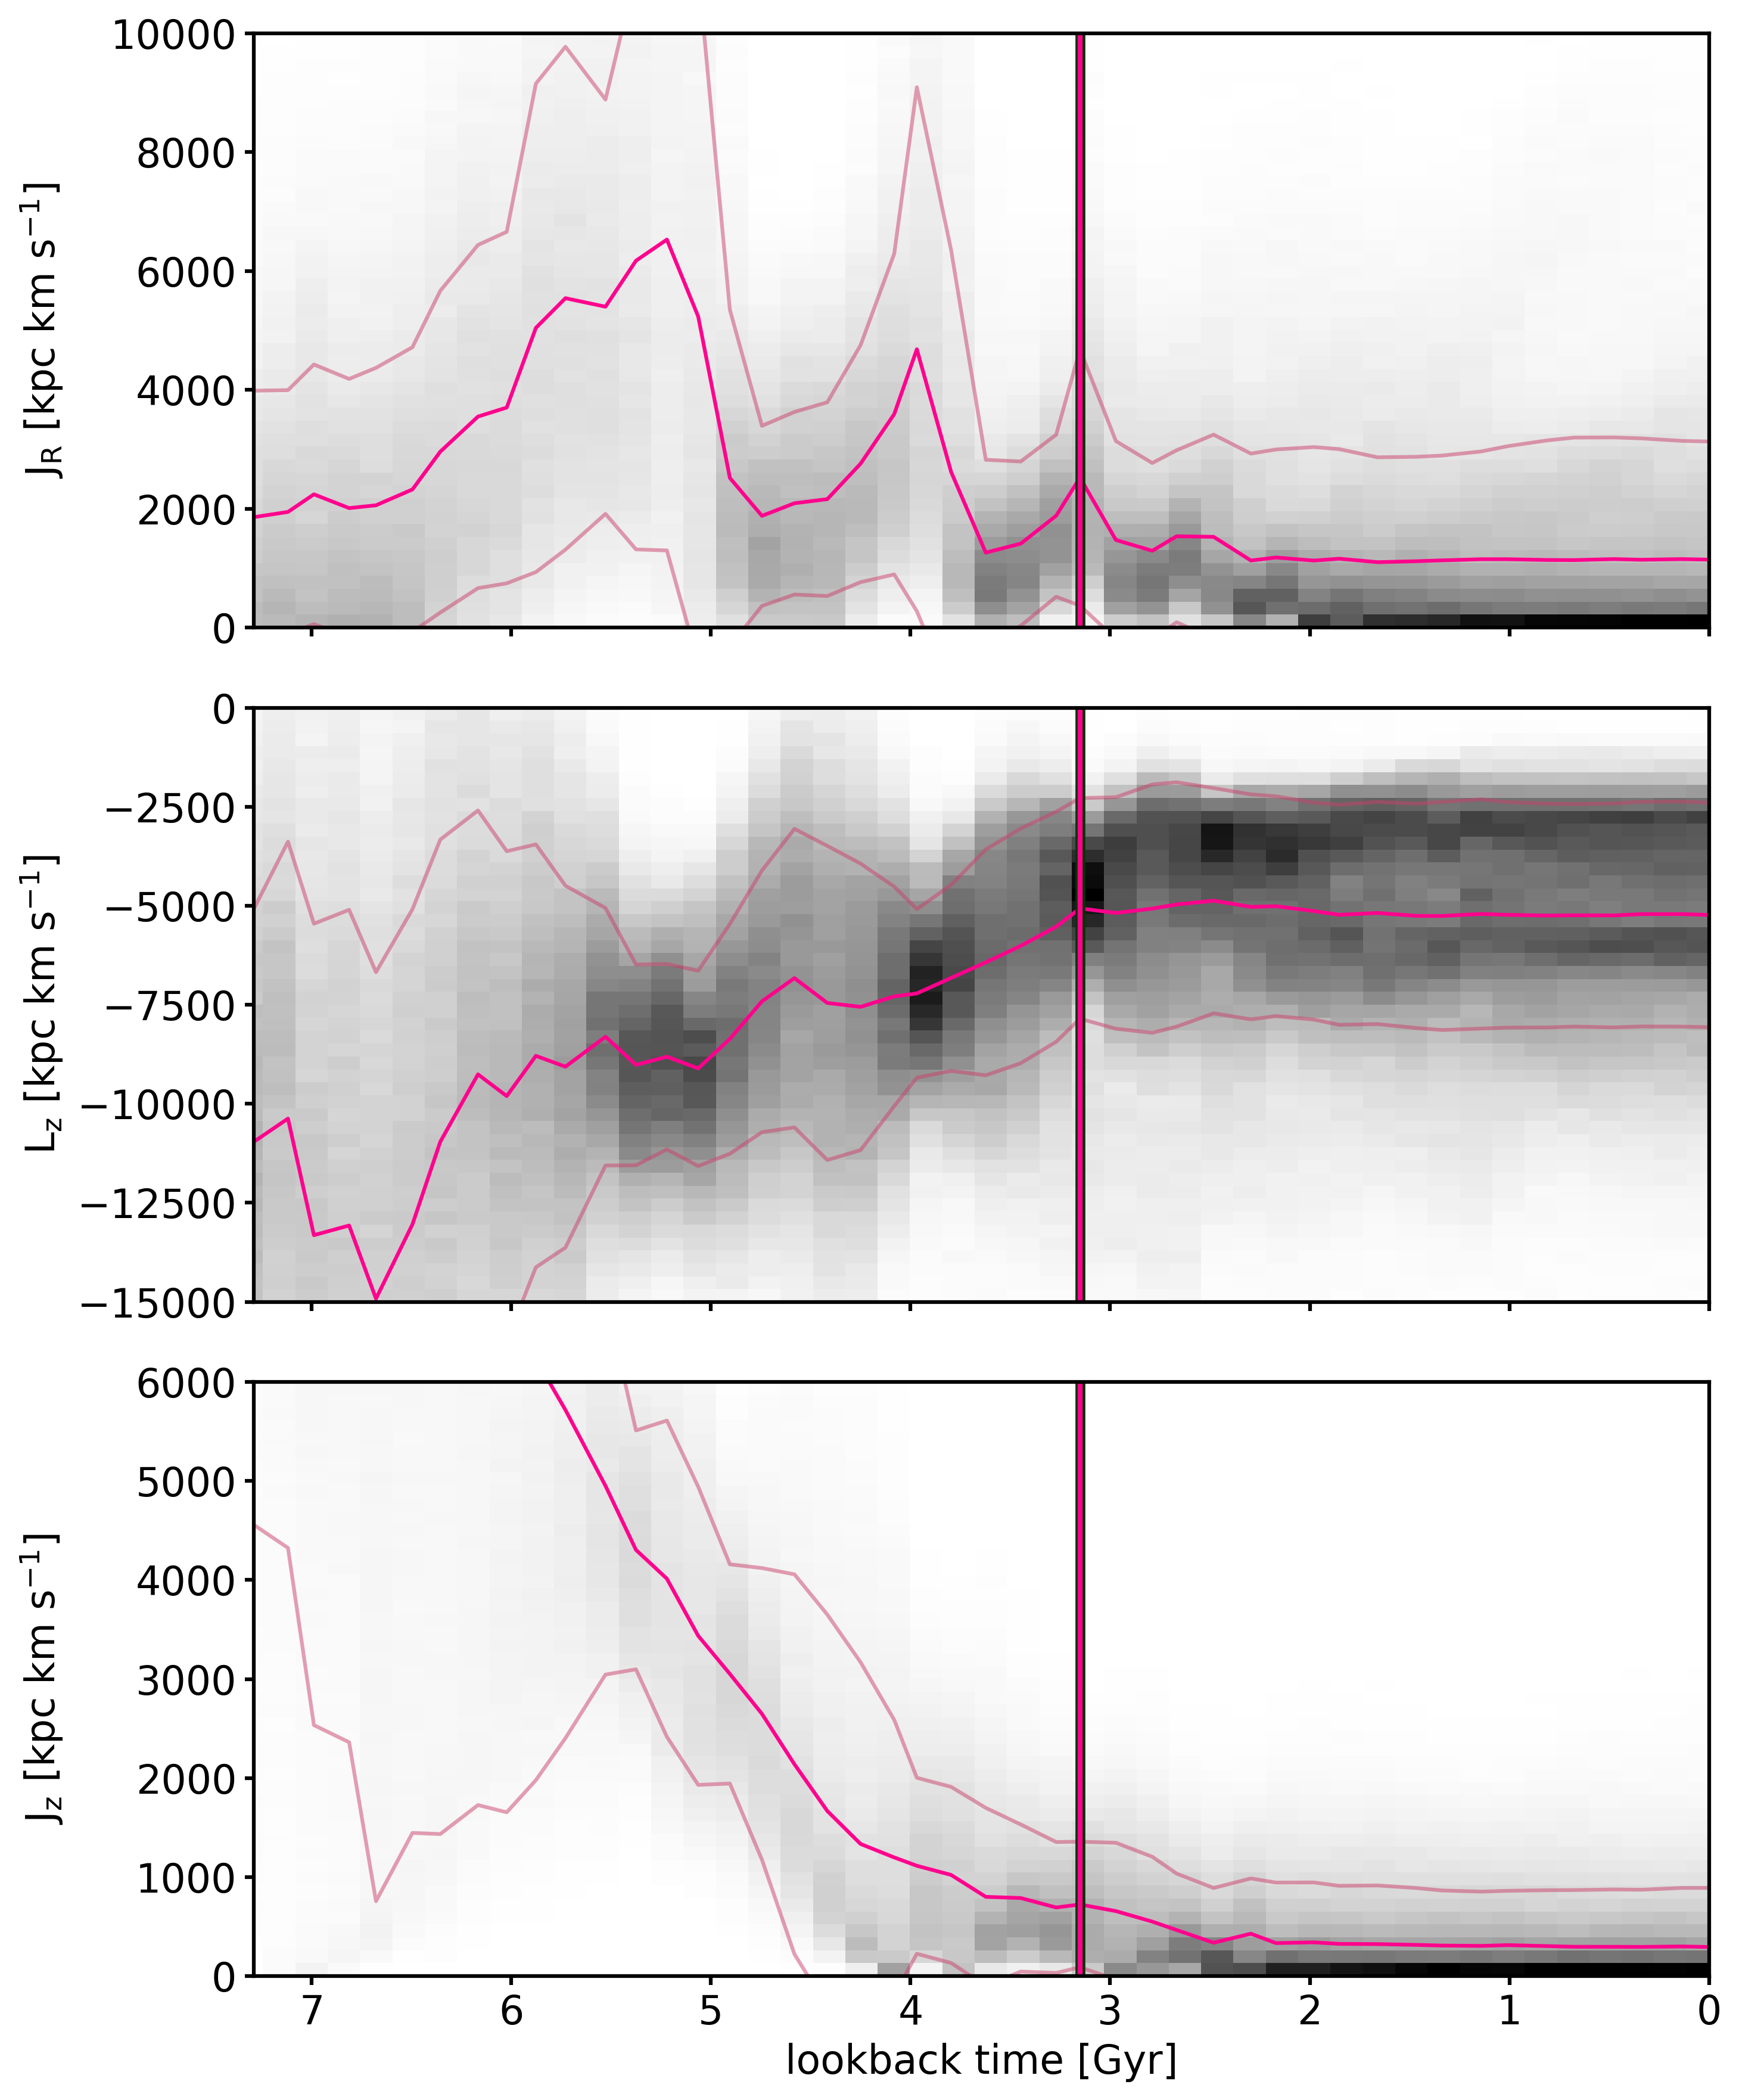
\includegraphics[width=\textwidth]{plots/Dynamics/prog2/action_time_evolution_wodisk_hist_mean.png}
    \end{subfigure}
    ~
    \begin{subfigure}[c]{0.48\textwidth}
    \centering
	    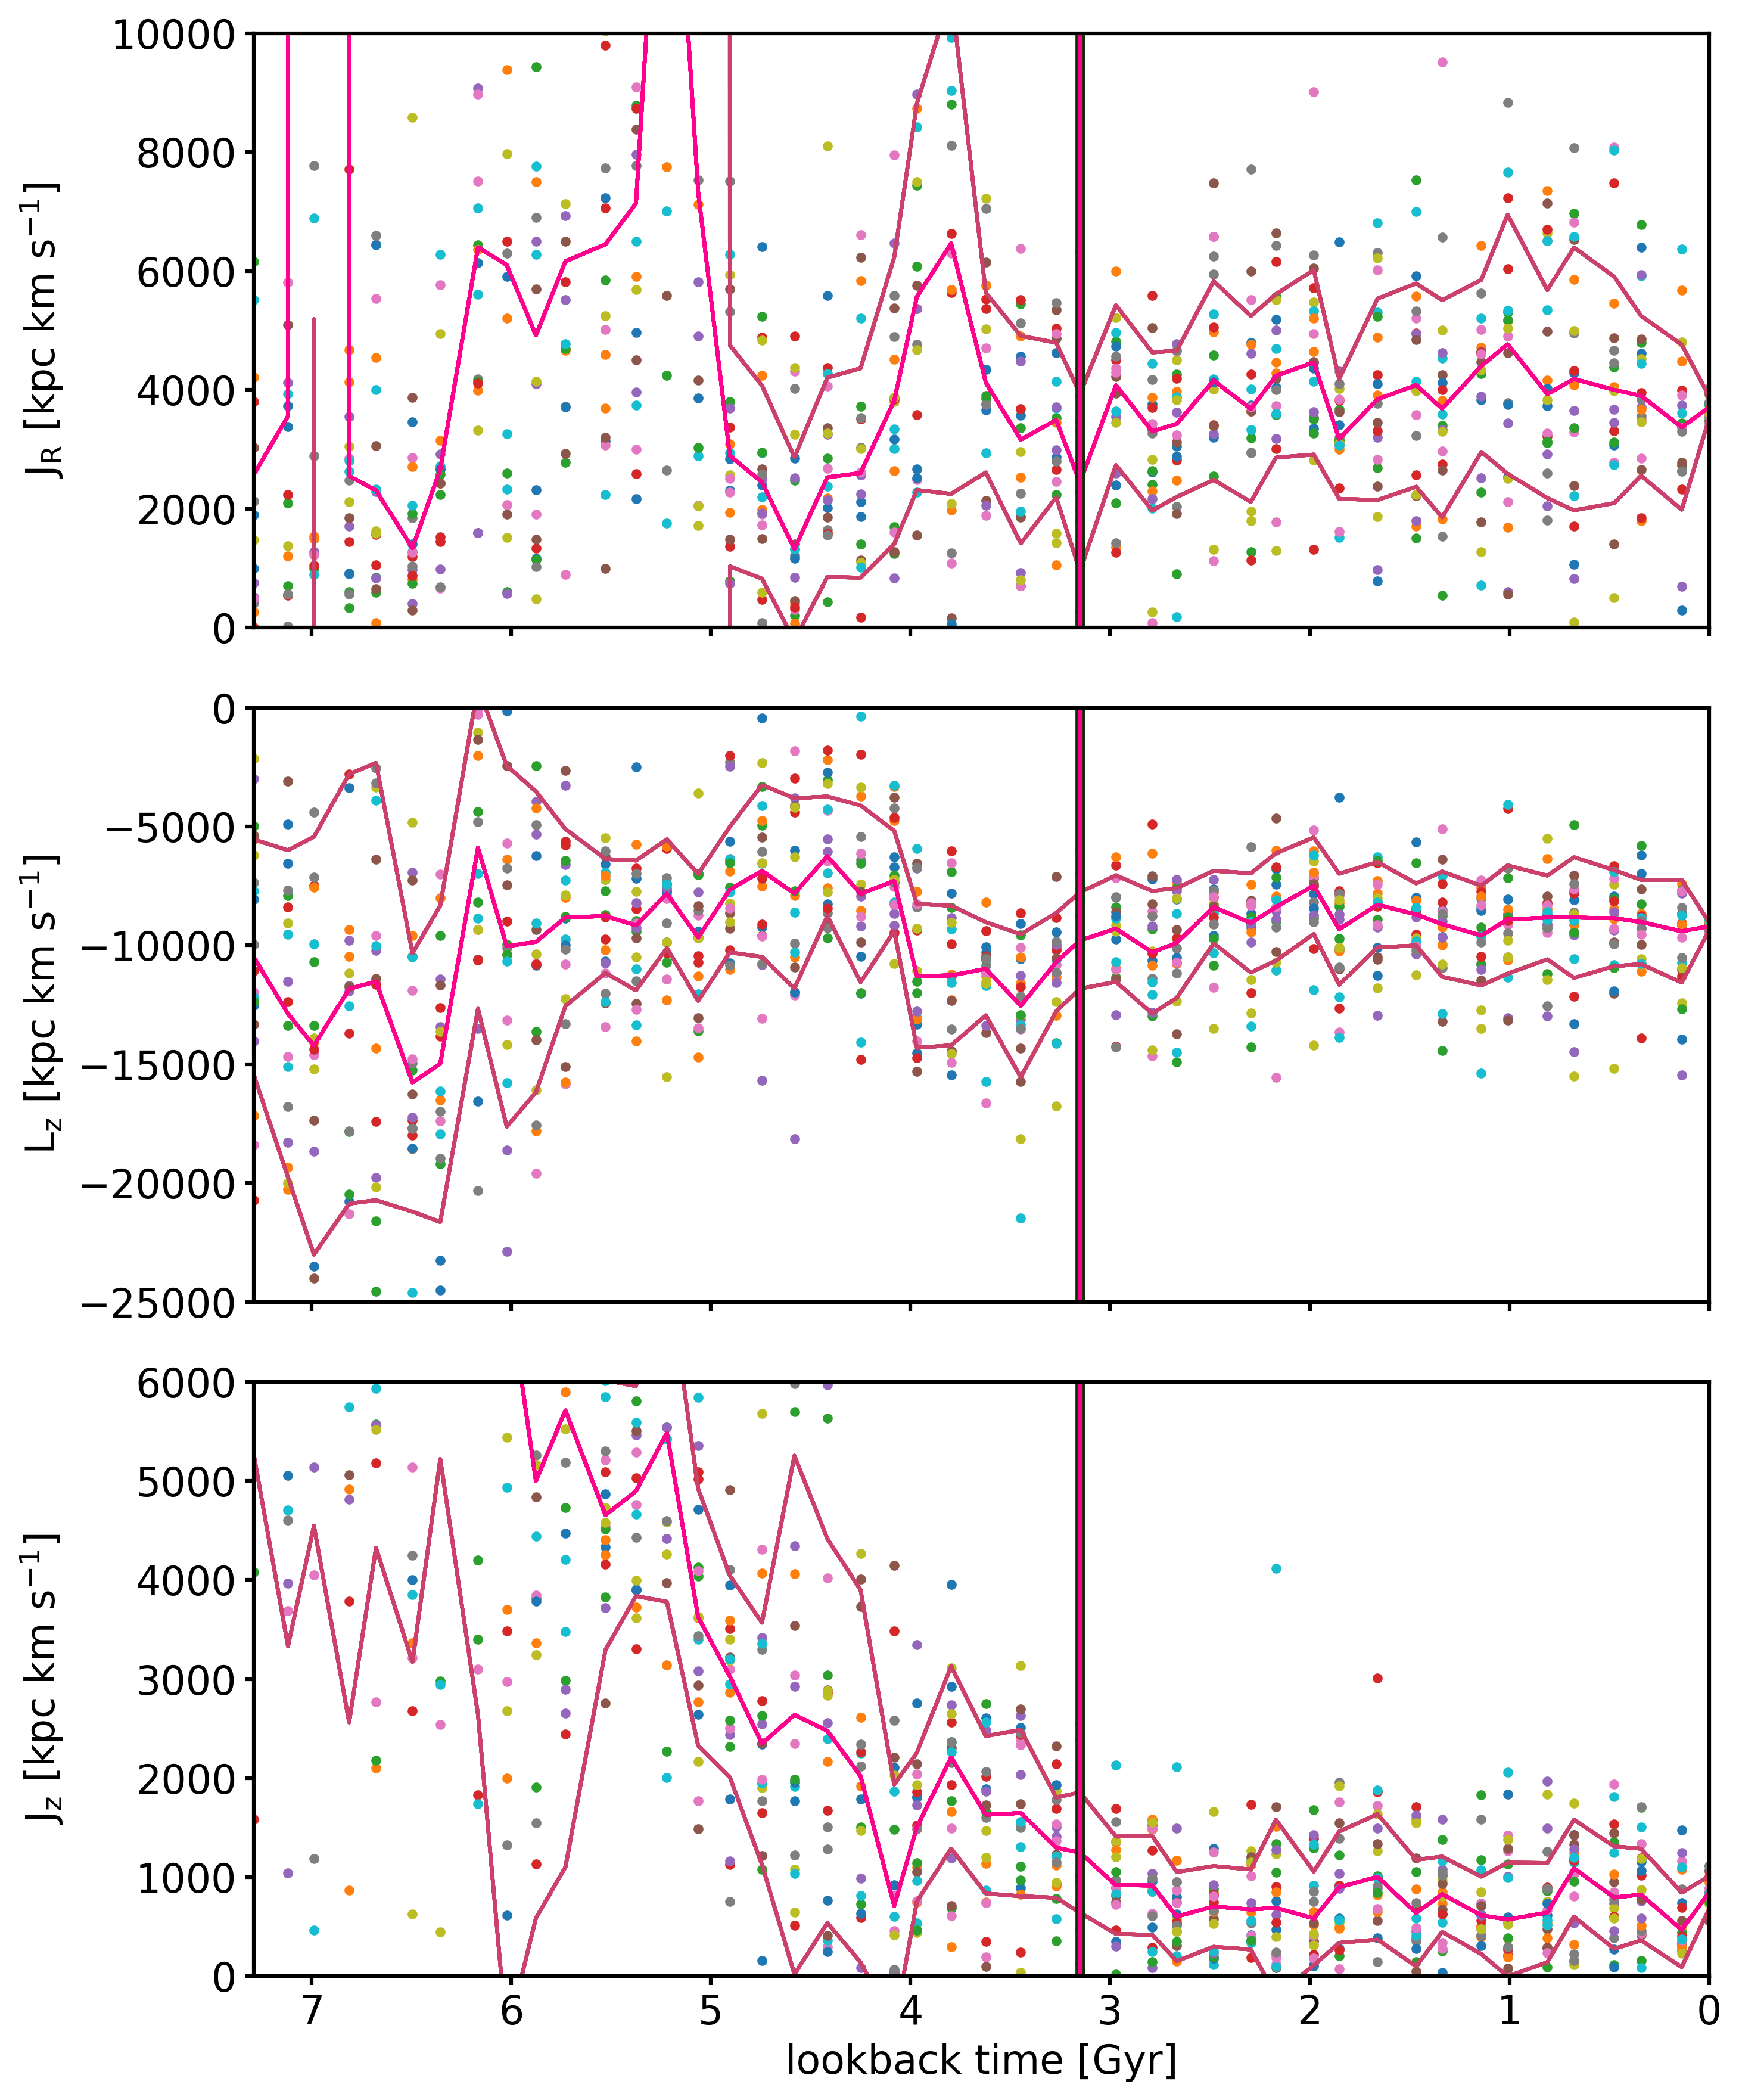
\includegraphics[width=\textwidth]{plots/Dynamics/prog2/action_time_evolution_box_hist_mean_prog2.png}
    \end{subfigure}
    \caption{\textcolor{red}{update with new selected GCs and therefore new boxcoming}}\label{fig:comparison_actions_time_evolution_box_prog2}
\end{figure}
In Figure \ref{fig:comparison_actions_box_time_evolution_prog2}, we plot the evolution of these actions in the right panel. At the last snapshot, we see how close they are in all three actions by construction. But already one snapshot before, they spread out widely and do not have any connection. Going back in time, the spread approximately stays constant. So even though we find similar orbit parameters at the very end, they do not evolve similarly. We compare the evolution of the box particles to the evolution of all accreted particles from prog2 in the left panel. The median and standard deviations evolve around the same values. \\\\
We constructed a case in which we find a few \acp{GC} on similar orbits at the current time as we find them in observations. These could be used to constrain the potential by minimizing their spread. \textcolor{red}{ irgendwie einmal nett formulieren in dieser subsection If we found \acp{GC} clumped together in actions today, they could have a similar evolution or would just be on the same orbit now by chance. }Looking at their time evolution leads to the conclusion that they are only on same orbits right now by chance and will have different properties soon again. So even if constraining the potential by minimizing the spread of accreted \acp{GC} in action would work we need to be careful in the selection of these \acp{GC}.
\iffalse
\begin{figure}
\captionsetup{format=plain}
    \centering
	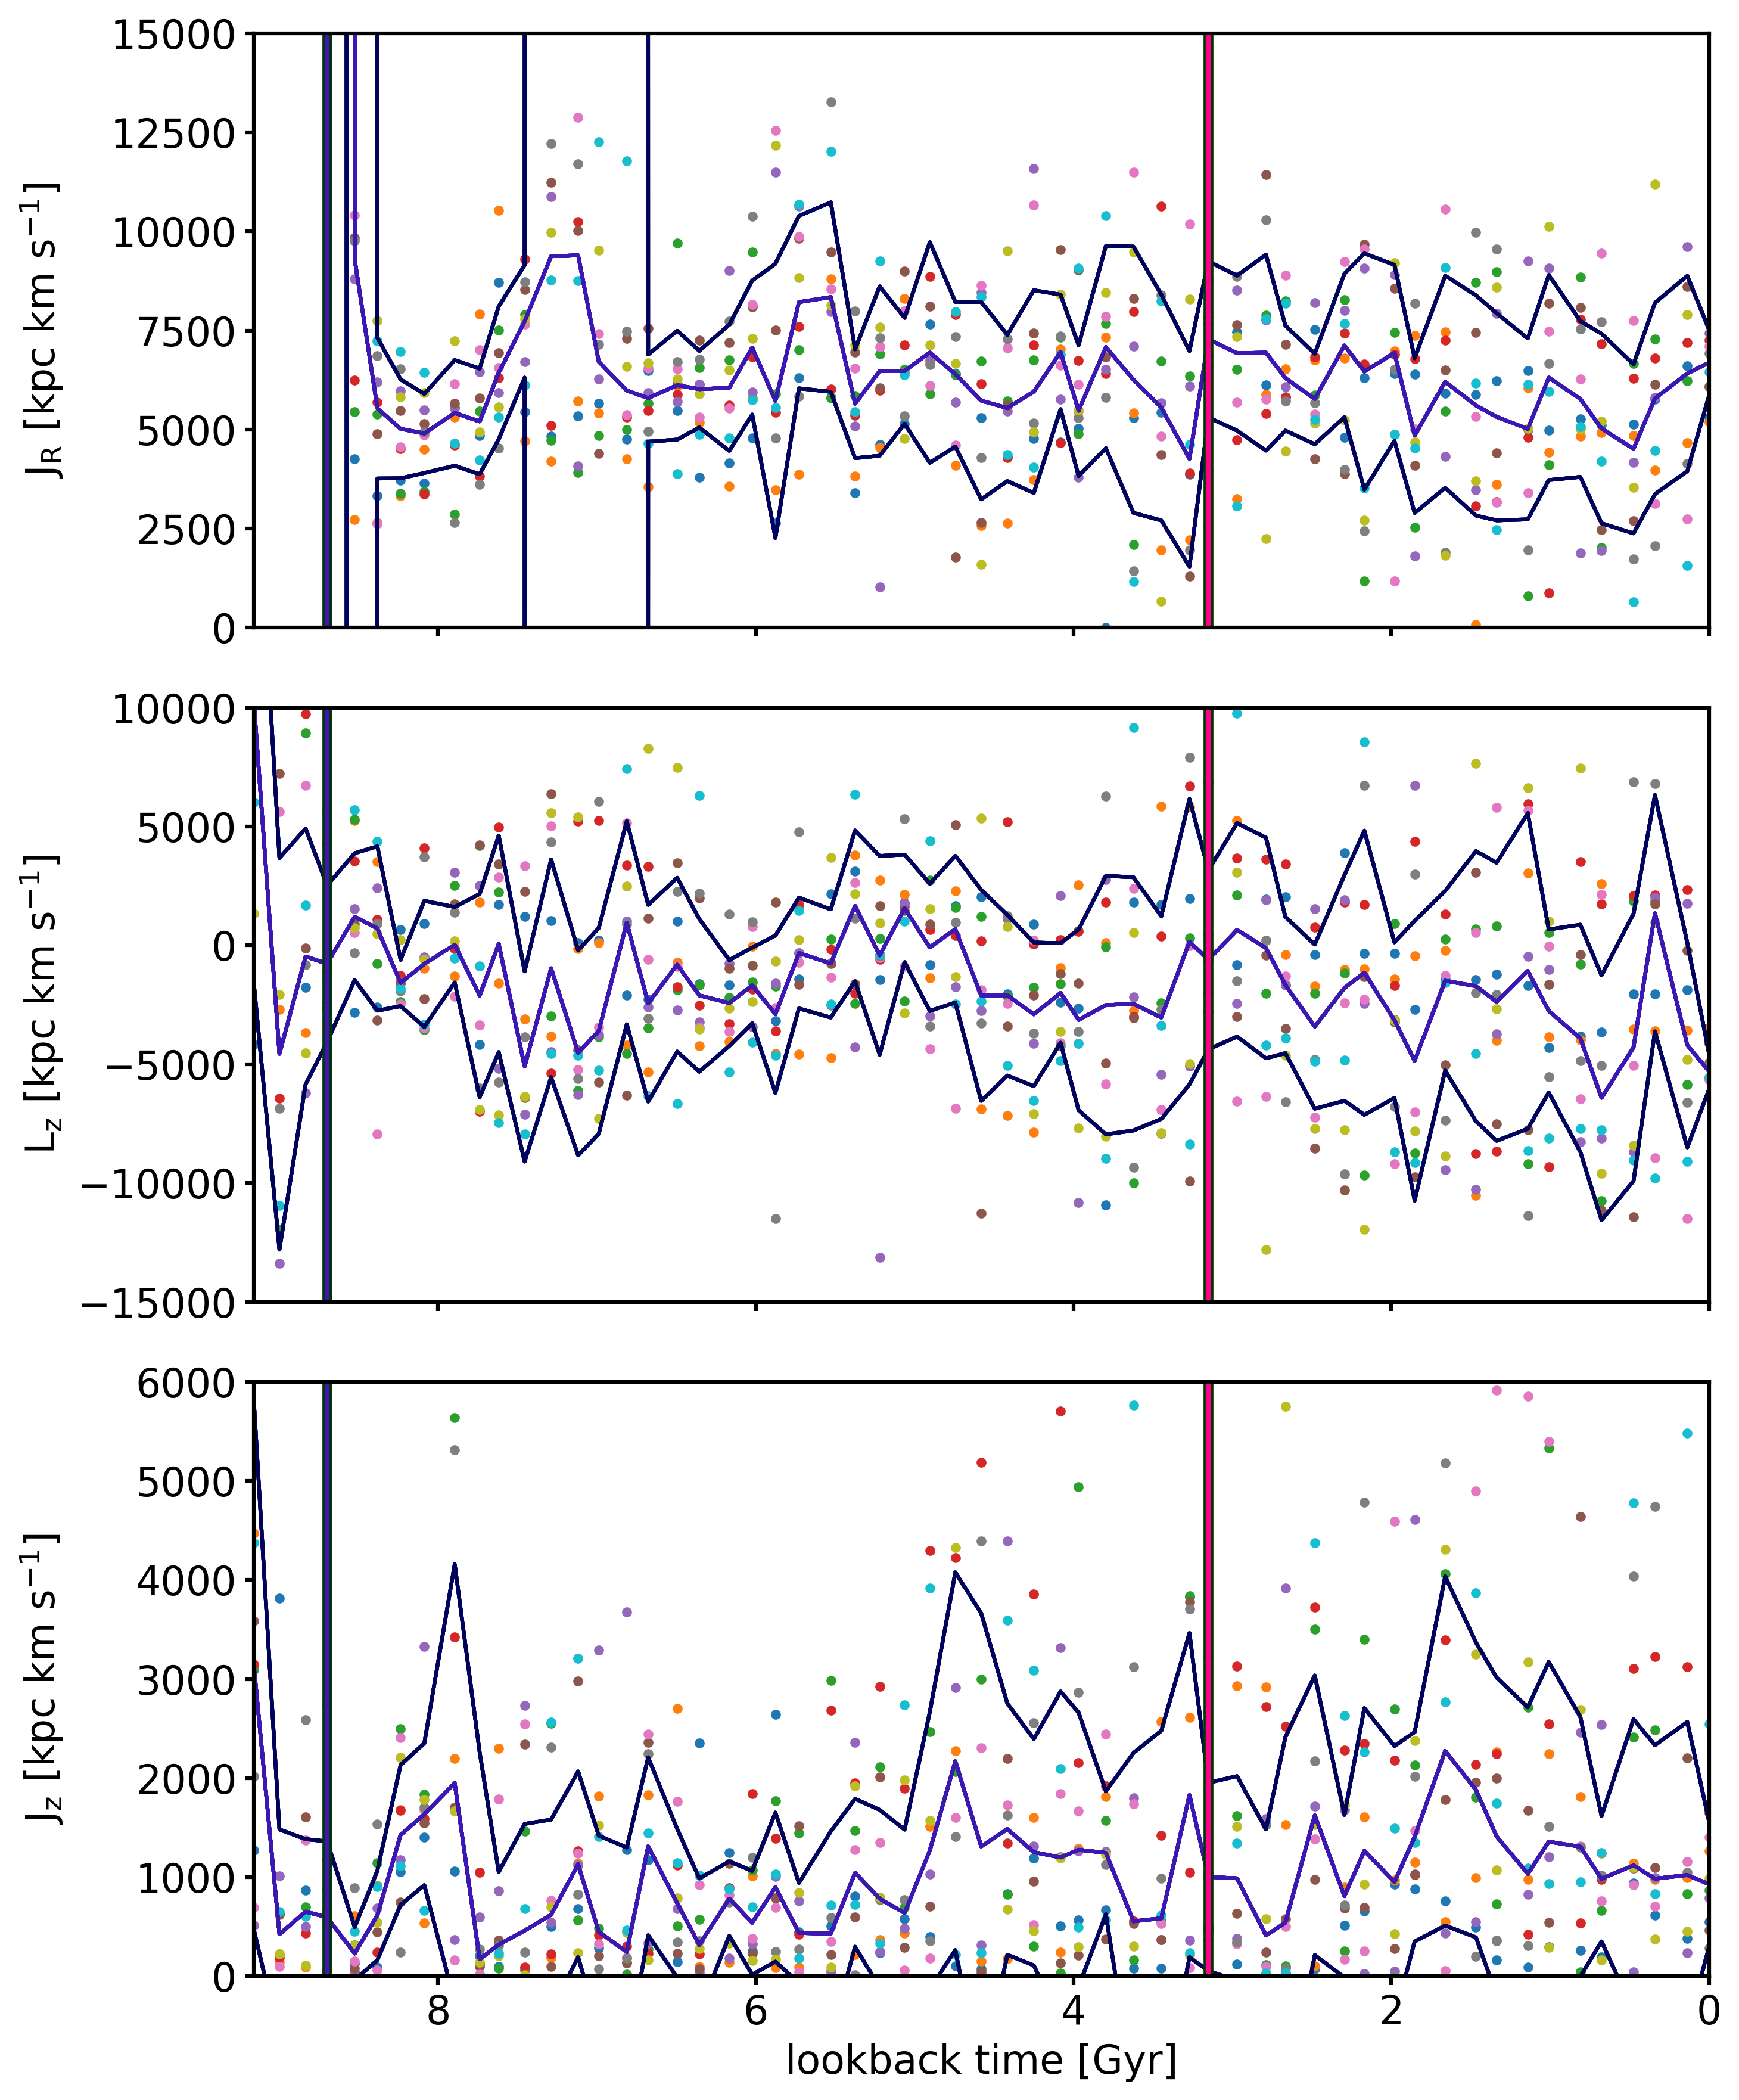
\includegraphics[width=\textwidth]{plots/Dynamics/prog3/action_time_evolution_box_hist_mean_prog3.png}
    \caption{Action time evolution of xx particles of prog3 which are found to be on similar orbits in the $z=0$ snapshot.}\label{fig:actions_box_time_evolution_prog3}
\end{figure}

\begin{figure}[htbp]
\captionsetup{format=plain}
    \centering
	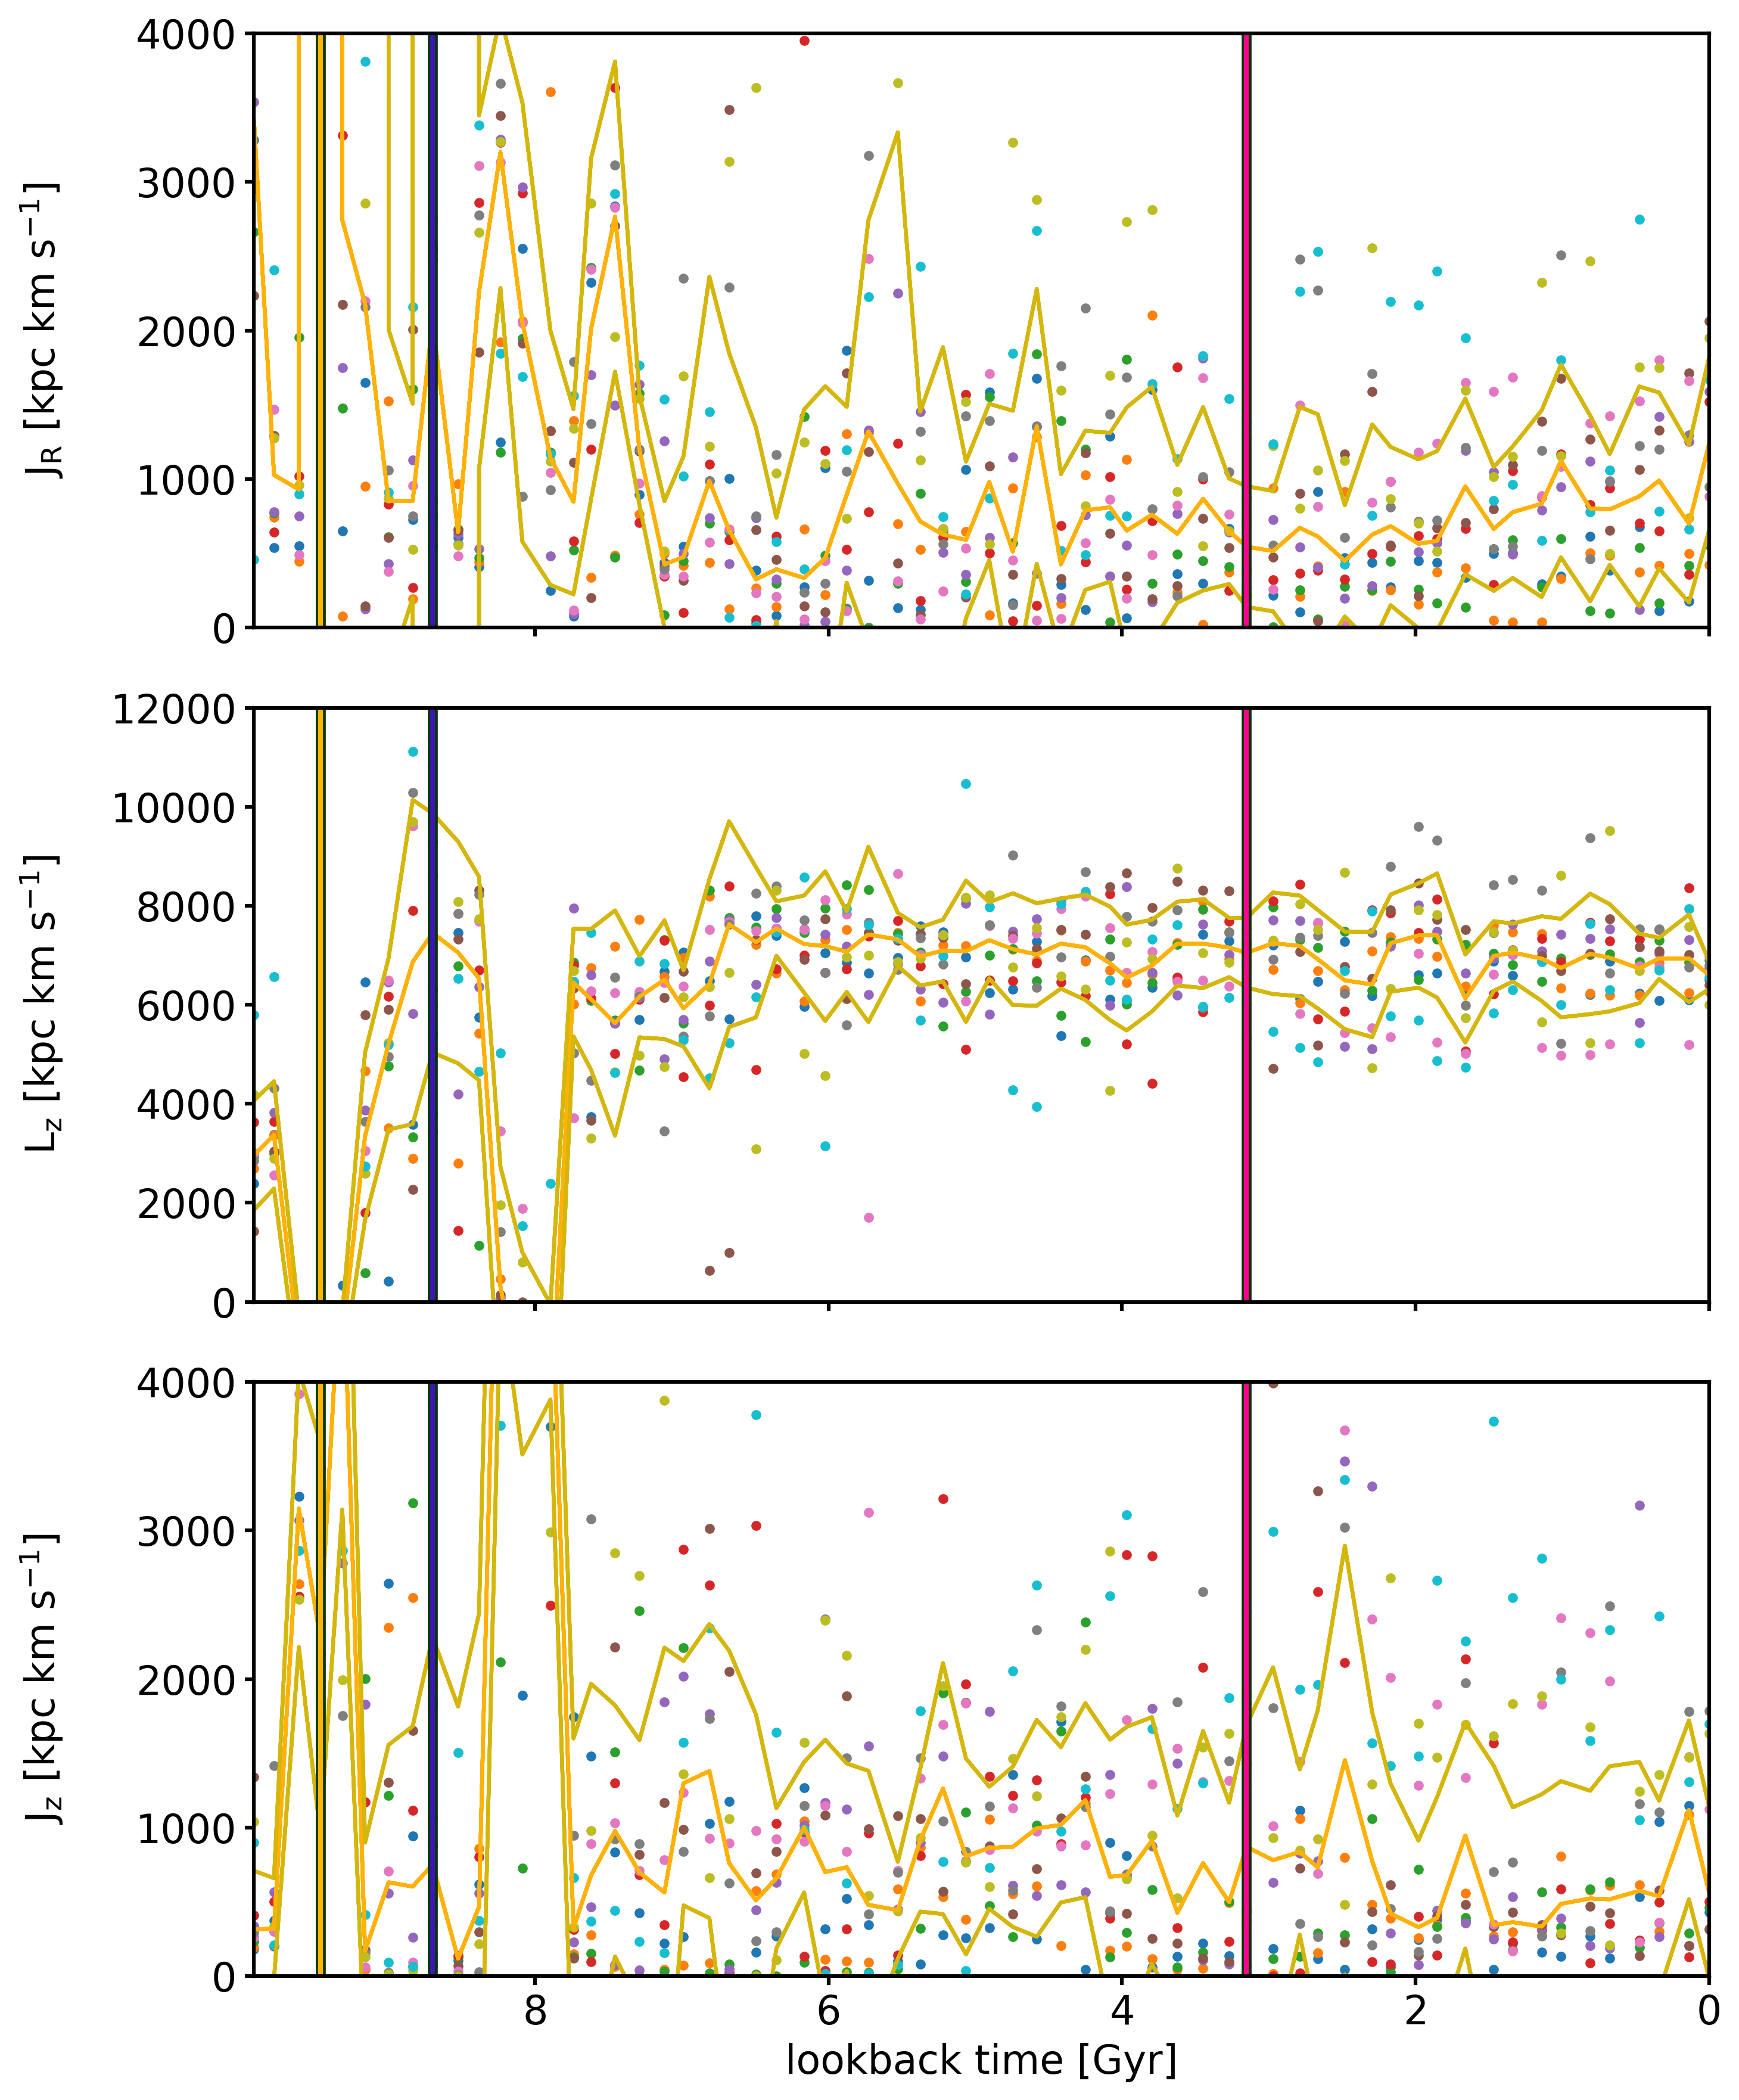
\includegraphics[width=\textwidth]{plots/Dynamics/prog4/action_time_evolution_box_hist_mean_prog4.png}
    \caption{Action time evolution of xx particles of prog4 which are on as similar orbits as possible. }\label{fig:actions_box_time_evolution_prog4}
\end{figure}
\fi



\section{Discussion} \label{sec:Discussion}
\subsection{Implications}
\textcolor{red}{Fazit + implications of my results in the bigger picture of research and science}
\\\\\textbf{Cold vs hot streams:}
The assumption that the \ac{DF} of accreted particles is a $\delta$-function in action space requires them to be on the same orbit - an assumption that is not fully \textcolor{red}{reference} but more closely \textcolor{red}{reference} satisfied for cold stellar streams. Already in the introduction we have mentioned, that \ac{DG} mergers usually create hot stellar streams so our particle streams in Auriga are dynamically hot and have a different, more complex \ac{DF}.

\subsection{Comparison to observations\textcolor{red}{better title}}
It is import to compare results from analysis simulations to observations. One test is looking at our Galaxy, where we have 6D phase space information available, e.g. with Gaia \citep{Gaia...mission...2016, GaiaDR2...overview...2018}, and to see how remnants of a \ac{DG} merger are distributed actions space.
\iffalse
\textbf{Excursion: coordinate transformations}
private communication with Wilma Trick
\fi
Recently, \textit{Gaia}-Enceladus \citep{Enceladus....Helmi...2018} \textcolor{red}{also put in references of sausage DG} was discovered in the \textit{Gaia} data. These are remnant stars of a merger approximately \SI{10}{Gyr} ago with a mass ratio of 0.24. In contrary to the Sagittarius \ac{DG} we have precise 6D information from \textit{Gaia} DR2 about Enceladus which we need to calculate the actions. The time of its merger is comparable to prog4.\textcolor{red}{more info on enceladus: what data; selection; coordinate trafo; potential assumption; discovery of enceladus}

\begin{figure}[htbp]
    \centering
    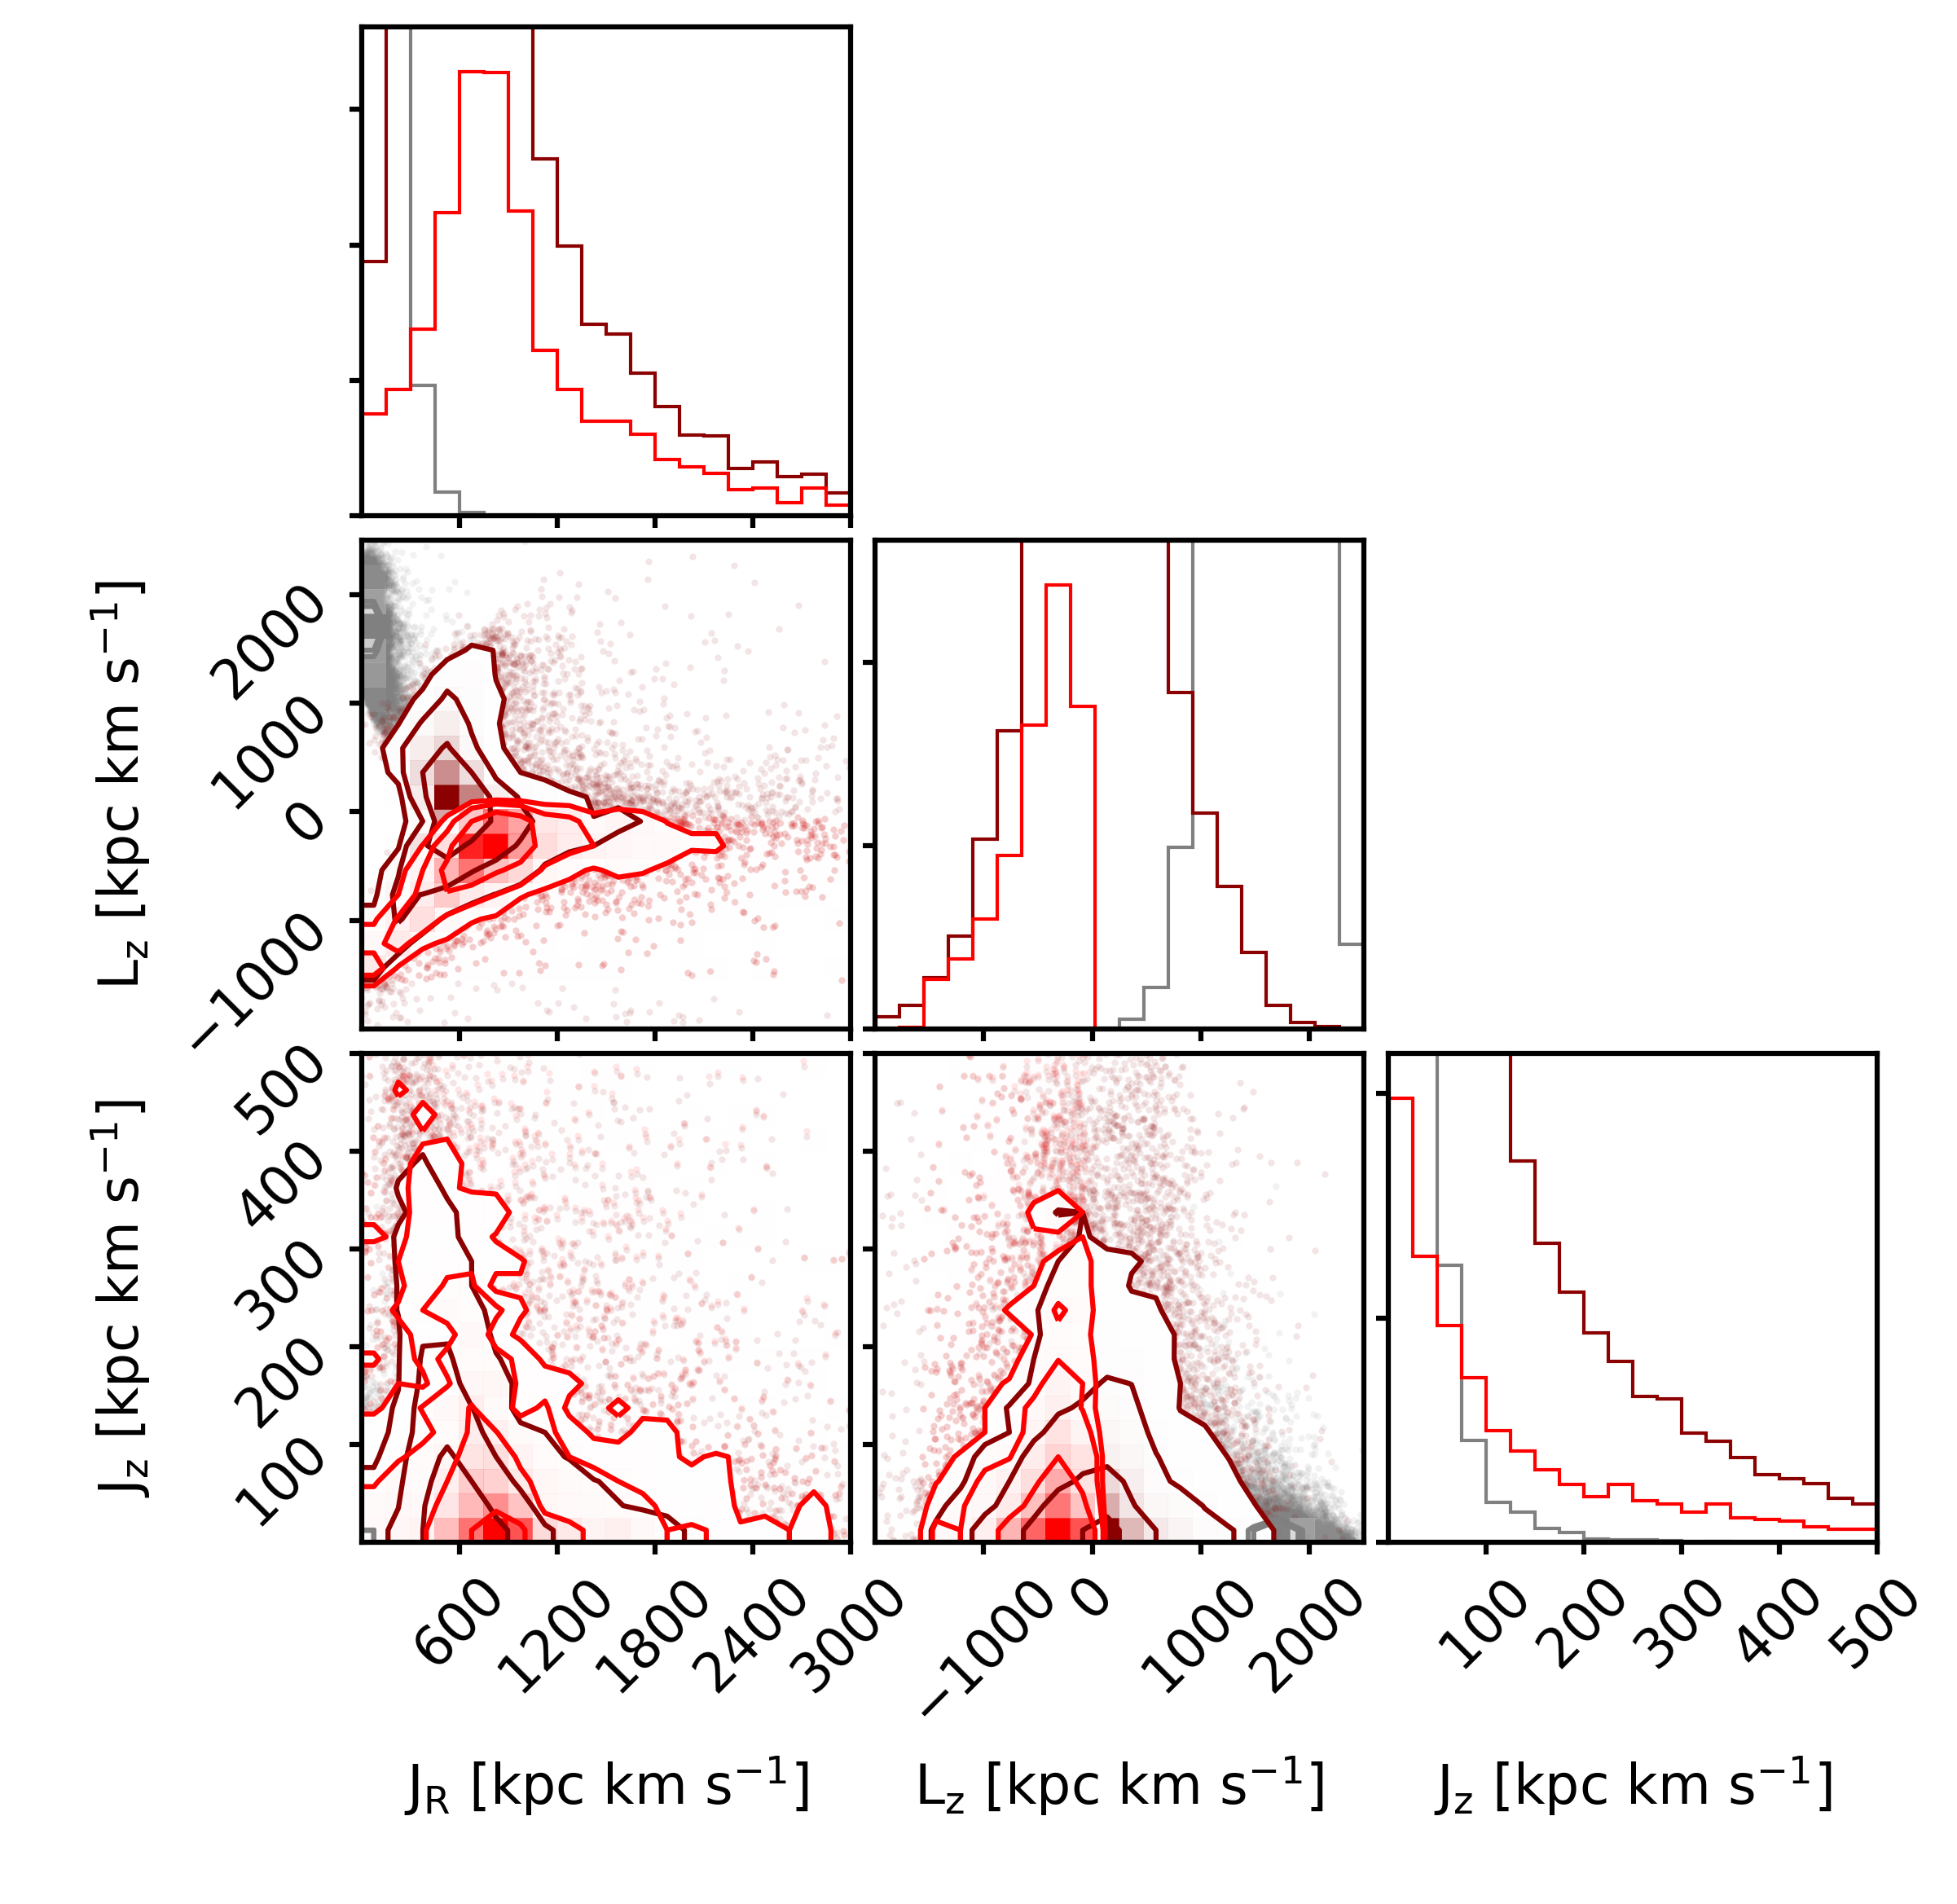
\includegraphics[width=1.0\textwidth]{plots/Discussion/Gaia_all_actions_MW14_talk3.png}
    \caption{\textit{Gaia}-Enceladus stars in action space in the MWPotential2014 \citep{Bovy...galpy...2015}. The data is taken from \textit{Gaia} DR2 \citep{GaiaDR2...overview...2018} in the \ac{MW} within \textcolor{red}{what distance $1/\omega <...kpc$}In grey, actions of disk stars are plotted. Dark red is the halo including some of the thick disk stars. \textit{Gaia}-Enceladus stars are plotted in red. Disk and halo are clearly distinguishable in angular momentum and also in radial action. \textit{Gaia}-Enceladus is not distinguishable from the halo as it makes up a significant part of it. It has a negative $L_z$ therefore it is counterrotating. It is also very spread out in action space so we cannot detect any sharp features.}
    \label{fig:Gaia_Enceladus_actions}
\end{figure}
We show in Figure \ref{fig:Gaia_Enceladus_actions} actions of the disk, halo and \textit{Gaia}-Enceladus. The remnants are neither distinguishable from the halo nor do they make a sharp feature in any of the actions. This tells us that even if there was more dynamical information contained in these stars shortly after the merger, this information vanishes over time. This confirms our findings that actions of objects accreted from a \ac{DG} merger cannot be seen as sharp features after some evolution. 


\subsection{Context in recent research and literature}
\textbf{\acp{GC} formation in cosmological simulations} Timo Halbesma (PhD student at the MPA) is working on extracting \acp{GC} in the Auriga simulations which have proper physical properties and physically motivated formation recipes. Repeating the same analysis in this work with a set of proper \acp{GC} could change our results. One reason could be that if we select properly surviving \acp{GC} they could clump in action space because their orbits might stay constant and therefore they could be used to tune the potential right.\\
The E-MOSAICS simulation suite \citep{Pfeffer...E-MOSAICS...2018, Kruijssen...E-MOSAICS.MW..2018} are zoom-in simulations of the cosmological EAGLE \citep{Schaye...EAGLE...2015} simulations which have implemented models describing the formation, evolution, and disruption of star clusters. In these simulations, Meghan Hughes (PhD student at ESO/LJMU) works on modelling the potential and Sebastian Trujillo-Gomez (Post-doc at ARI) investigates the kinematics of the \acp{GC}. 
\\\\
\textbf{Constraining gravitational potential}
\textcolor{red}{sorry muss hier noch in die literatur schauen}
There are attempts of applying adaptive dynamics or dynamical modelling with \acp{GC} to the \ac{MW}.
\begin{itemize}
    \item \textbf{\acp{DF} of \acp{GC}} \citep{Posti...MWmassGCs...2018}
    looked at all GCs and did not differentiate bw in-situ/ex-situ and coming from differetn \acp{DG}
    \item \textbf{Sharpen stellar streams in sims to find true potential} \citep{Sanderson...streams..adaptivedyn...2015, Sanderson...gravpotstreams...2017}
\end{itemize}
\citet{Jean-Baptiste...accactionspace...2017}

\subsection{Caveats}
\textcolor{red}{too harsh}This work and its results cannot be blindly trusted. There are a few assumptions and problems in the course of the investigations which might have influenced the results.
\\\\\textbf{GC selection:}
One of the main problems in the analysis is the \acp{GC} selection. Auriga does not resolve \acp{GC} and therefore we need to make assumptions and select \ac{GC} candidates. We applied a very simple recipe which only excluded simulated particles as \ac{GC} candidates which were in a snapshot in a regime where the stellar disk was very dense \textcolor{red}{Wilma has an idea how to show strong disk forces; if time ask her} and could have destroyed the \ac{GC} \textcolor{red}{reference for GC destroyed in disk}. \textcolor{red}{check the next sentence; try to better describe the specific not random selection} When selecting only a subset of the \acp{GC}, we have very different statistics of each progenitor group, e.g. the means shift significantly. A proper, physical selection would make these results more reliable. \textcolor{red}{what could be considered in the physical selection of GCs and why is this not in Auriga}
\\\\\textbf{Potential fit:}
As we have discussed in Section \ref{subsec:wrong_pot_fit}, there are a few problems with the potential fit. The bulge-disk decomposition probably underestimates the disk and creates a flaring spatial selection effect. For each component, the model differs from the data especially in the center. This is due to the choice of binning the data, fitting routines, the assumption of spherical or axisymmetry, the simplified potential model consisting of only three analytic building blocks etc. In total, the potential is good enough for the course of our investigations but, as one of the next steps, should be improved.

\subsection{Future Work}
There are a lot of things which we could not investigate or we had to make compromises on due to the time limitations of this thesis. Big issues which we already discussed are with the potential model and with the \ac{GC} selection. Improving these recipes would make our analysis more robust. \textcolor{red}{ideas on improvement; check if/what i have mentioned in sec 2.3 and repeat it quickly}
\\\\
\texttt{galpy} and \texttt{AGAMA} \citep{Vasiliev...AGAMA...2019} can in principle calculate actions for \textit{N}-body simulations directly without the need of an analytic gravitational potential. We should compare if the action distribution and evolution behaves as we measured because of their nature and their physical evolution in the simulation (so direct calculation of actions and calculating them in the potential model would give similar results) or because a analytic axisymmetric potential (in general or only our fit) cannot well describe the real potential and messes these things up. Up to now, it was not possible to do this step because of technical issues. 

\\\\The final goal would be to find the right \ac{DF} of accreted particles which is not yet possible due to numerical (and observational) limitations. If we had that, adaptive dynamics in external galaxies should be a useful method to constrain their gravitational potential. With this true \ac{DF} and the right gravitational potential, we would know everything about the dynamics of the galaxy.



\fancyhf{}
\fancyhead{}
\fancyhead[RO,LE]{5. Summary \& conclusion}
\fancyfoot{}
\fancyfoot[LE,RO]{\thepage}
\fancyfoot[LO,RE]{}
\section{Summary and conclusion}\label{sec:sumconc}

We did 
\begin{itemize}
    \item 
\end{itemize}

\newpage
\fancyhf{}
\fancyhead{}
\fancyhead[RO,LE]{Acronyms}
\fancyfoot{}
\fancyfoot[LE,RO]{\thepage}
\fancyfoot[LO,RE]{}
\section*{Acronyms}
\addcontentsline{toc}{section}{Acronyms}

\begin{acronym}[WIMPs]
    \acro{AGN}{active galactic nuclei}
    \acro{AMR}{age-metallicity relation}
    \acro{CBE}{collisionless Boltzmann equation}
    \acro{CDM}{cold dark matter}
    \acro{CMB}{cosmic microwave background}
    \acro{DF}{distribution function}
    \acro{DG}{dwarf galaxy}
	\acro{DM}{dark matter}
	\acro{DMO}{dark matter only}
	\acro{D/T}{disk-to-total}
	\acro{GC}{globular cluster}
	\acro{HST}{Hubble Space Telescope}
	\acro{IFU}{Integral Field Unit}
	\acro{IoM}[IoMs]{integrals of motion}
	\acro{LCDM}[$\Lambda$CDM]{Lambda cold dark matter}
	\acro{LG}{Local Group}
	\acro{MGE}{Multi-Gaussian Expansion}
	\acro{MHD}{magnetohydrodynamical}
	\acro{ML}[M/L]{mass-to-light}
	\acro{MN}{Miyamoto-Nagai}
	\acro{MoND}{Modified Newtonian Dynamics}
	\acro{MW}{Milky Way}
	\acro{NFW}{Navarro-Frenk-White}
	\acro{PM}{proper motion}
	\acro{TF}{Tully-Fisher}
	\acro{WDM}{warm dark matter}
	\acro{WIMPs}{Weakly Interacting Massive Particles}

\end{acronym}
\newpage

\fancyhf{}
\fancyhead{}
\fancyhead[RO,LE]{References}
\fancyfoot{}
\fancyfoot[LE,RO]{\thepage}
\fancyfoot[LO,RE]{}
\addcontentsline{toc}{section}{References}

\bibliography{mybib}{}
%\bibliographystyle{mnras}
\newpage
\addcontentsline{toc}{section}{Acknowledgements}
\thispagestyle{plain}
\section*{Thank you,}

\textbf{Glenn van de Ven}, for giving me the opportunity to join you at ESO, to work again in the exciting field of dynamics, 

\textbf{Ralf Klessen}, for evaluating my thesis.

\textbf{Wilma Trick},

\textbf{Timo Halbesma}, for helping me with all the technical things and for proofreading that part of my thesis.

\textbf{Laura Watkins and Prashin Jethwa}, for proofreading my thesis and for advice on my science and applications.

\textbf{Volker Springel}, for providing me with the excellent Auriga simulations.

\textbf{Jo Bovy}, for providing galpy which I heavily used for my investigations.

\textbf{The European Southern Observatory and the “Galaxy Dynamics” research group in Heidelberg and Garching}, for providing such a friendly and scientifically inspiring environment and many helpful colleagues.

\textbf{The European Research Council}, for funding from the European Research Council (ERC) under the European Union's Horizon 2020 research and innovation programme under grant agreement No 724857 (Consolidator Grant ArcheoDyn).

\textbf{the "ESO 5th floor"}, for making my time at ESO fun and happy.

\textbf{my parents Sigrun and Ivo}, for supporting me in everything.

\textbf{my brother and best friend Niko}, for always being there.
\newpage
\addcontentsline{toc}{section}{Statement}
\thispagestyle{plain}
\section*{Statement}
\setlength{\parindent}{0em}

\vspace{3\baselineskip}
This thesis is my own work and I have only used the sources indicated. Where the work of others has been quoted or reproduced, the source is always given.\par
\vspace{5\baselineskip}
Heidelberg, January 18, 2019\hspace{3cm}\dotfill




\end{document}
